% Options for packages loaded elsewhere
\PassOptionsToPackage{unicode}{hyperref}
\PassOptionsToPackage{hyphens}{url}
%
\documentclass[
  12pt,
]{article}
\usepackage{amsmath,amssymb}
\usepackage{lmodern}
\usepackage{iftex}
\ifPDFTeX
  \usepackage[T1]{fontenc}
  \usepackage[utf8]{inputenc}
  \usepackage{textcomp} % provide euro and other symbols
\else % if luatex or xetex
  \usepackage{unicode-math}
  \defaultfontfeatures{Scale=MatchLowercase}
  \defaultfontfeatures[\rmfamily]{Ligatures=TeX,Scale=1}
\fi
% Use upquote if available, for straight quotes in verbatim environments
\IfFileExists{upquote.sty}{\usepackage{upquote}}{}
\IfFileExists{microtype.sty}{% use microtype if available
  \usepackage[]{microtype}
  \UseMicrotypeSet[protrusion]{basicmath} % disable protrusion for tt fonts
}{}
\makeatletter
\@ifundefined{KOMAClassName}{% if non-KOMA class
  \IfFileExists{parskip.sty}{%
    \usepackage{parskip}
  }{% else
    \setlength{\parindent}{0pt}
    \setlength{\parskip}{6pt plus 2pt minus 1pt}}
}{% if KOMA class
  \KOMAoptions{parskip=half}}
\makeatother
\usepackage{xcolor}
\IfFileExists{xurl.sty}{\usepackage{xurl}}{} % add URL line breaks if available
\IfFileExists{bookmark.sty}{\usepackage{bookmark}}{\usepackage{hyperref}}
\hypersetup{
  pdftitle={Factors affecting reliablity of state-space age-structured assessment models},
  pdfauthor={Timothy J. Miller1; A. Applegate; G. Britten; E. N. Brooks; G. Fay; A. Hansell; C. M. Legault; B. Muffley; J. Wiedenmann},
  hidelinks,
  pdfcreator={LaTeX via pandoc}}
\urlstyle{same} % disable monospaced font for URLs
\usepackage[margin=1in]{geometry}
\usepackage{graphicx}
\makeatletter
\def\maxwidth{\ifdim\Gin@nat@width>\linewidth\linewidth\else\Gin@nat@width\fi}
\def\maxheight{\ifdim\Gin@nat@height>\textheight\textheight\else\Gin@nat@height\fi}
\makeatother
% Scale images if necessary, so that they will not overflow the page
% margins by default, and it is still possible to overwrite the defaults
% using explicit options in \includegraphics[width, height, ...]{}
\setkeys{Gin}{width=\maxwidth,height=\maxheight,keepaspectratio}
% Set default figure placement to htbp
\makeatletter
\def\fps@figure{htbp}
\makeatother
\setlength{\emergencystretch}{3em} % prevent overfull lines
\providecommand{\tightlist}{%
  \setlength{\itemsep}{0pt}\setlength{\parskip}{0pt}}
\setcounter{secnumdepth}{5}
\newlength{\cslhangindent}
\setlength{\cslhangindent}{1.5em}
\newlength{\csllabelwidth}
\setlength{\csllabelwidth}{3em}
\newlength{\cslentryspacingunit} % times entry-spacing
\setlength{\cslentryspacingunit}{\parskip}
\newenvironment{CSLReferences}[2] % #1 hanging-ident, #2 entry spacing
 {% don't indent paragraphs
  \setlength{\parindent}{0pt}
  % turn on hanging indent if param 1 is 1
  \ifodd #1
  \let\oldpar\par
  \def\par{\hangindent=\cslhangindent\oldpar}
  \fi
  % set entry spacing
  \setlength{\parskip}{#2\cslentryspacingunit}
 }%
 {}
\usepackage{calc}
\newcommand{\CSLBlock}[1]{#1\hfill\break}
\newcommand{\CSLLeftMargin}[1]{\parbox[t]{\csllabelwidth}{#1}}
\newcommand{\CSLRightInline}[1]{\parbox[t]{\linewidth - \csllabelwidth}{#1}\break}
\newcommand{\CSLIndent}[1]{\hspace{\cslhangindent}#1}
\usepackage{url}
\usepackage{setspace}
%\singlespacing
%\onehalfspacing
\doublespacing
\usepackage{lineno}
\linenumbers
\usepackage[belowskip=0pt,aboveskip=0pt]{caption}
\usepackage{relsize}
\newcommand{\Fmsy}{\ensuremath{F_{\text{MSY}}}\xspace}
\newcommand{\Fspr}[1]{\ensuremath{F_{\text{{#1}\%}}}\xspace}
\newcommand{\afrb}{Alaska Fishery Research Bulletin\xspace}
\newcommand{\ajms}{African Journal of Marine Science\xspace}
\newcommand{\amb}{Advances in Marine Biology\xspace}
\newcommand{\bms}{Bulletin of Marine Science\xspace}
\newcommand{\bjssf}{Bulletin of the Japanese Society of Scientific Fisheries\xspace}
\newcommand{\cb}{Conservation Biology\xspace}
\newcommand{\cjfas}{Canadian Journal of Fisheries and Aquatic Sciences\xspace}
\newcommand{\ea}{Ecological Applications\xspace}
\newcommand{\eer}{Evolutionary Ecology Research\xspace}
\newcommand{\elet}{Ecology Letters\xspace}
\newcommand{\emod}{Ecological Modelling\xspace}
\newcommand{\ebf}{Environmental Biology of Fishes\xspace}
\newcommand{\ff}{Fish and Fisheries\xspace}
\newcommand{\fo}{Fisheries Oceanography\xspace}
\newcommand{\fr}{Fisheries Research\xspace}
\newcommand{\fb}{Fishery Bulletin\xspace}
\newcommand{\ijms}{ICES Journal of Marine Science\xspace}
\newcommand{\iccat}{Collective Volume of Scientific Papers ICCAT\xspace}
\newcommand{\jae}{Journal of Animal Ecology\xspace}
\newcommand{\jai}{Journal of Applied Ichthyology\xspace}
\newcommand{\jdc}{Journal Du Conseil International Pour L'exploration De La Mer\xspace}
\newcommand{\jdcp}{Journal Du Conseil Permanent International Pour L'exploration De La Mer\xspace}
\newcommand{\jembe}{Journal of Experimental Marine Biology and Ecology\xspace}
\newcommand{\jfb}{Journal of Fish Biology\xspace}
\newcommand{\jsr}{Journal of Sea Research\xspace}
\newcommand{\jtb}{Journal of Theoretical Biology\xspace}
\newcommand{\jfrbc}{Journal of the Fisheries Research Board of Canada\xspace}
\newcommand{\jnwafs}{Journal of Northwest Atlantic Fisheries Science\xspace}
\newcommand{\mcf}{Marine and Coastal Fisheries: Dynamics, Management, and Ecosystem Science\xspace}
\newcommand{\mb}{Marine Biology\xspace}
\newcommand{\meps}{Marine Ecology Progress Series\xspace}
\newcommand{\mfr}{Marine Fisheries Review\xspace}
\newcommand{\mpb}{Marine Pollution Bulletin\xspace}
\newcommand{\najfm}{North American Journal of Fisheries Management\xspace}
\newcommand{\nzjmfr}{New Zealand Journal of Marine and Freshwater Research\xspace}
\newcommand{\pnas}{Proceedings of the National Academy of Sciences USA\xspace}
\newcommand{\rpvrciemm}{Rapports et Proc\`es-Verbaux des R\'eunions. Conseil Internationale pour l'Exploration de la Mer\xspace}
\newcommand{\rpvrcpiemm}{Rapports et Proc\`es-Verbaux des R\'eunions. Conseil Permanent Internationale pour l'Exploration de la Mer\xspace}
\newcommand{\rfbf}{Reviews in Fish Biology and Fisheries\xspace}
\newcommand{\sajms}{South African Journal of Marine Science\xspace}
\newcommand{\tafs}{Transactions of the American Fisheries Society\xspace}

\newcommand{\anzjs}{Australian \& New Zealand Journal of Statistics\xspace}
\newcommand{\as}{Applied Statistics\xspace}
\newcommand{\csda}{Computational Statistics \& Data Analysis\xspace}
\newcommand{\ees}{Environmental and Ecological Statistics\xspace}
\newcommand{\jas}{Journal of Applied Statistics\xspace}
\newcommand{\jabes}{Journal of Agricultural, Biological, and Environmental Statistics\xspace}
\newcommand{\jasa}{Journal of the American Statistical Association\xspace}
\newcommand{\jrssb}{Journal of the Royal Statistical Society. Series B\xspace}
\newcommand{\sm}{Statistics in Medicine}

\usepackage{xspace}
\usepackage{bm}
\usepackage{caption,graphics}
\usepackage{graphicx}
\usepackage{makecell}
\renewcommand\figurename{Fig.}
\captionsetup{labelsep=period, singlelinecheck=false}
\newcommand{\changesize}[1]{\fontsize{#1pt}{#1pt}\selectfont}
\renewcommand{\arraystretch}{1.5}
\renewcommand\theadfont{}
\usepackage{booktabs}
\usepackage{longtable}
\usepackage{array}
\usepackage{multirow}
\usepackage{wrapfig}
\usepackage{float}
\usepackage{colortbl}
\usepackage{pdflscape}
\usepackage{tabu}
\usepackage{threeparttable}
\usepackage{threeparttablex}
\usepackage[normalem]{ulem}
\usepackage{makecell}
\usepackage{xcolor}
\ifLuaTeX
  \usepackage{selnolig}  % disable illegal ligatures
\fi
\usepackage[]{natbib}
\bibliographystyle{cjfas2.bst}

\title{Factors affecting reliablity of state-space age-structured
assessment models}
\author{Timothy J. Miller\textsuperscript{1} \and A. Applegate \and G.
Britten \and E. N. Brooks \and G. Fay \and A. Hansell \and C. M.
Legault \and B. Muffley \and J. Wiedenmann}
\date{}

\begin{document}
\maketitle

\(^1\)corresponding author:
\href{mailto:timothy.j.miller@noaa.gov}{\nolinkurl{timothy.j.miller@noaa.gov}},
Northeast Fisheries Science Center, Woods Hole Laboratory, 166 Water
Street, Woods Hole, MA 02543 USA\\

\pagebreak

\hypertarget{abstract}{%
\subsection*{Abstract}\label{abstract}}
\addcontentsline{toc}{subsection}{Abstract}

\hypertarget{keywords}{%
\subsubsection*{Keywords}\label{keywords}}
\addcontentsline{toc}{subsubsection}{Keywords}

\pagebreak

\hypertarget{introduction}{%
\section*{Introduction}\label{introduction}}
\addcontentsline{toc}{section}{Introduction}

Application of state-space models in fisheries stock assessment and
management has expanded dramatically within ICES, Canada and the
Northeast US \citep{nielsenberg14,cadigan16,stockmiller21}. State-space
approaches that use random effects to parameterize process errors is
considered best practice and a requirement for the next generation of
stock assessment models.

Much is known about the reliability of state-space models that are
linear or Gaussian \citep{aeberhardetal18}, but applications in
fisheries management are nonlinear and typically include multiple types
of observations with varying distributional assumptions. Furthermore,
there is a wide range of potential random effects structures and model
parameters that can be treated as random effects in assessment models.
We know relatively little about the statistical reliability of such
models or the ability of information criteria to distinguish among such
alternative structures.

Convergence results can be useful for understanding how bad convergence
in applications to real data might direct the practitioner to which
alternative random effects configurations is be more appropriate. The
type of convergence that we might use as a diagnostic is important. And
what rule of thumb we use for certain criteria e.g.~1e-6? large SEs/CVs?

Here we conduct a simulation study with operating models varying by
degree of observation error uncertainty, sources of process error (M,
NAA, q, sel), and fishing history. The simulations from these operating
models are fitted with estimating models that make alternative
assumptions for sources of process error (M, NAA\textless{} q, sel),
whether a stock-recruit model was estimated, and whether M is estimated.
We evaluate whether AIC can correctly determine the correct source of
process error and stock effects on recruitment. We also evaluate the
degree of bias in the outputs of the assessment model that are important
for management.

\hypertarget{methods}{%
\section*{Methods}\label{methods}}
\addcontentsline{toc}{section}{Methods}

Used the WHAM package \citep[][commit 77bbd94]{stockmiller21} (Miller
and Stock 2020). This packages has also been used to configure operating
and estimating models for closed loop simulations evaluating index-based
assessment methods \citep{legaultetal23} and is used for management of
haddock, butterfish, plaice, bluefish in the Northeast US.

We completed a simulation study with a number of operating models that
can be categorized based on where process error random effects are
assumed: abundance at age (R, R+S), natural mortality (R+M), fleet
selectivity (R+Sel), or index catchability (R+q). For each operating
model assumptions about variance of process errors and observations are
required and the values we used were based on a review of the range of
estimates from recent applications of WHAM in management of stocks of
haddock, butterfish, and American plaice in the NE US.

78 total operating models. We simulated 100 data sets for each operating
model. For each simulated data set we fit a set of 20 estimating models.

\hypertarget{operating-models}{%
\subsection*{Operating models}\label{operating-models}}
\addcontentsline{toc}{subsection}{Operating models}

\hypertarget{population}{%
\subsubsection*{Population}\label{population}}
\addcontentsline{toc}{subsubsection}{Population}

The population model tracks 10 age classes: ages 1 to 10+ and we assume
spawning occurs 1/4 of the way through the year. The maturity at age was
a logistic curve with a50 = 2.89 and slope = 0.88 and assumed known in
all estimation models (Figure \ref{om_maturity}).

\begin{figure}
\caption{The proportion mature at age assumed for the population in all operating and estimating models.}\label{om_maturity}
\begin{center}
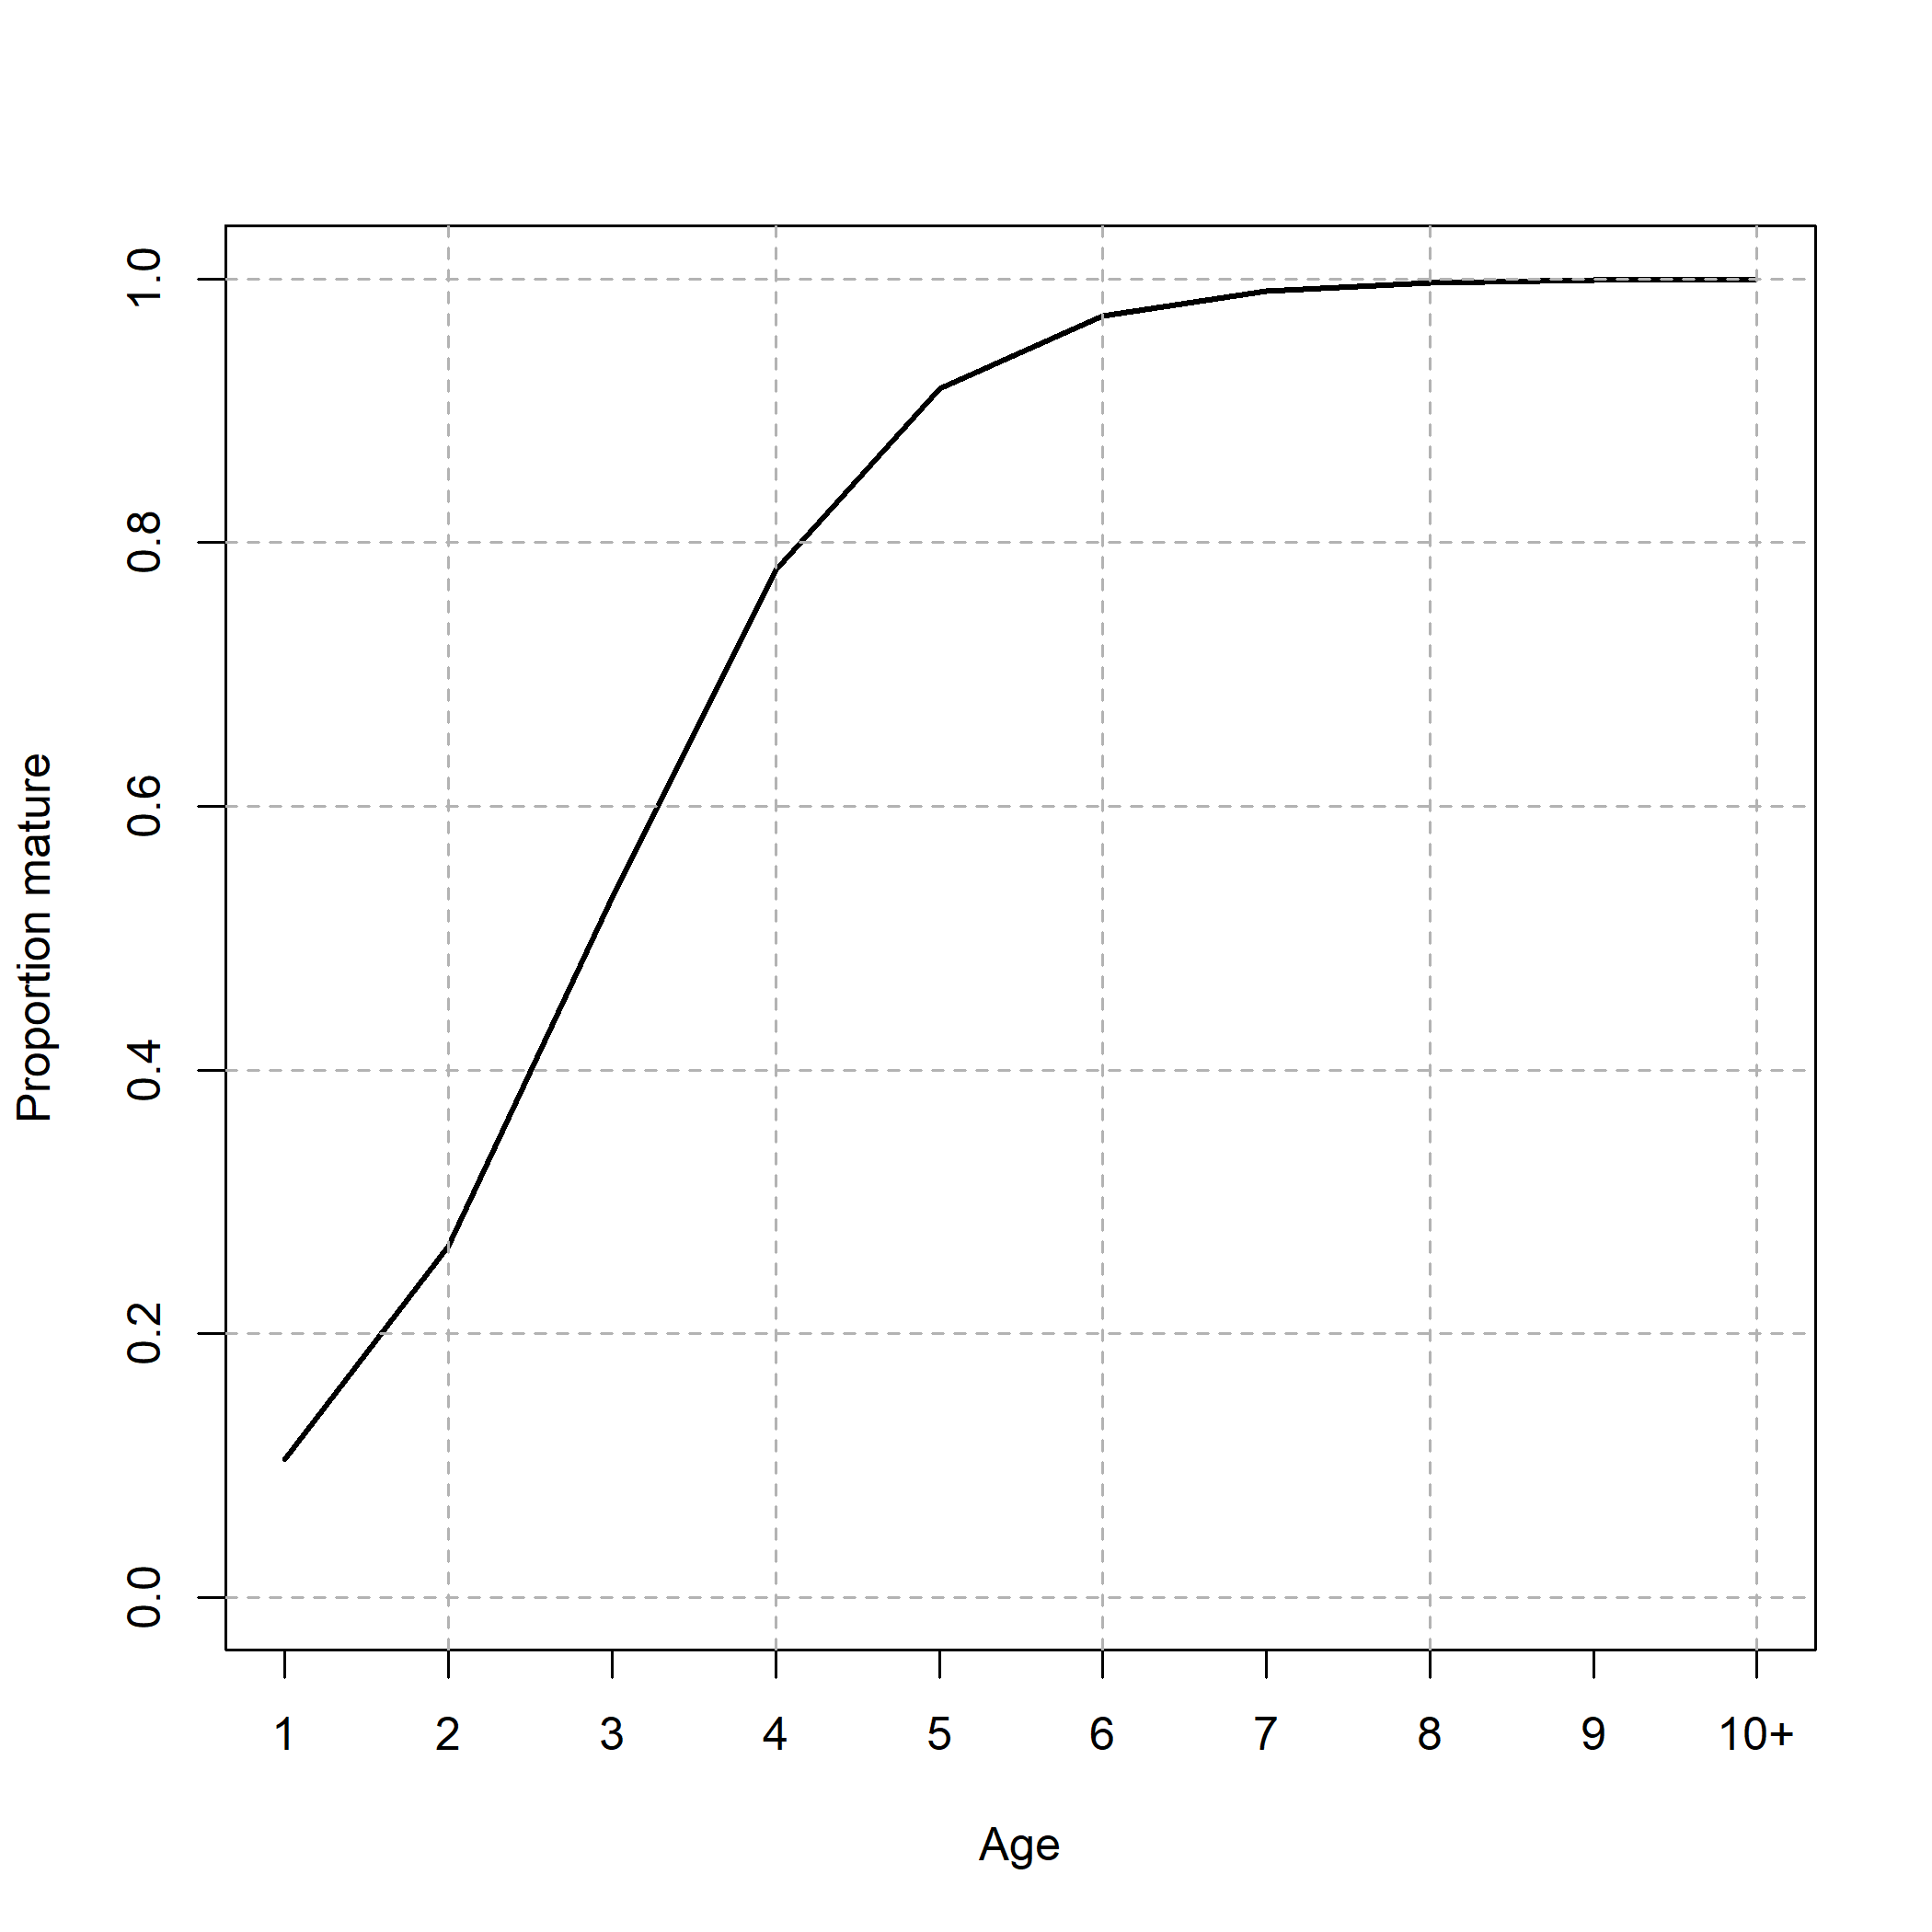
\includegraphics[width = \textwidth]{om_maturity.png}
\end{center}
\end{figure}

Weight at age was generated with a LVB growth function \[
L_a = L_{\infty}\left(1 - e^{-k(a - t_0)}\right)
\] where \(t_0 = 0\), \(L_\infty = 85\), and \(k = 0.3\), and a L-W
relationship such that \[
W_a = \theta_1 L_a^{\theta_2}
\] where \(\theta_1 = e^{-12.1}\) and \(\theta_2 = 3.2\) (Figure
\ref{om_waa}).

\begin{figure}
\caption{The weight at age assumed for the population in all operating and estimating models.}\label{om_waa}
\begin{center}
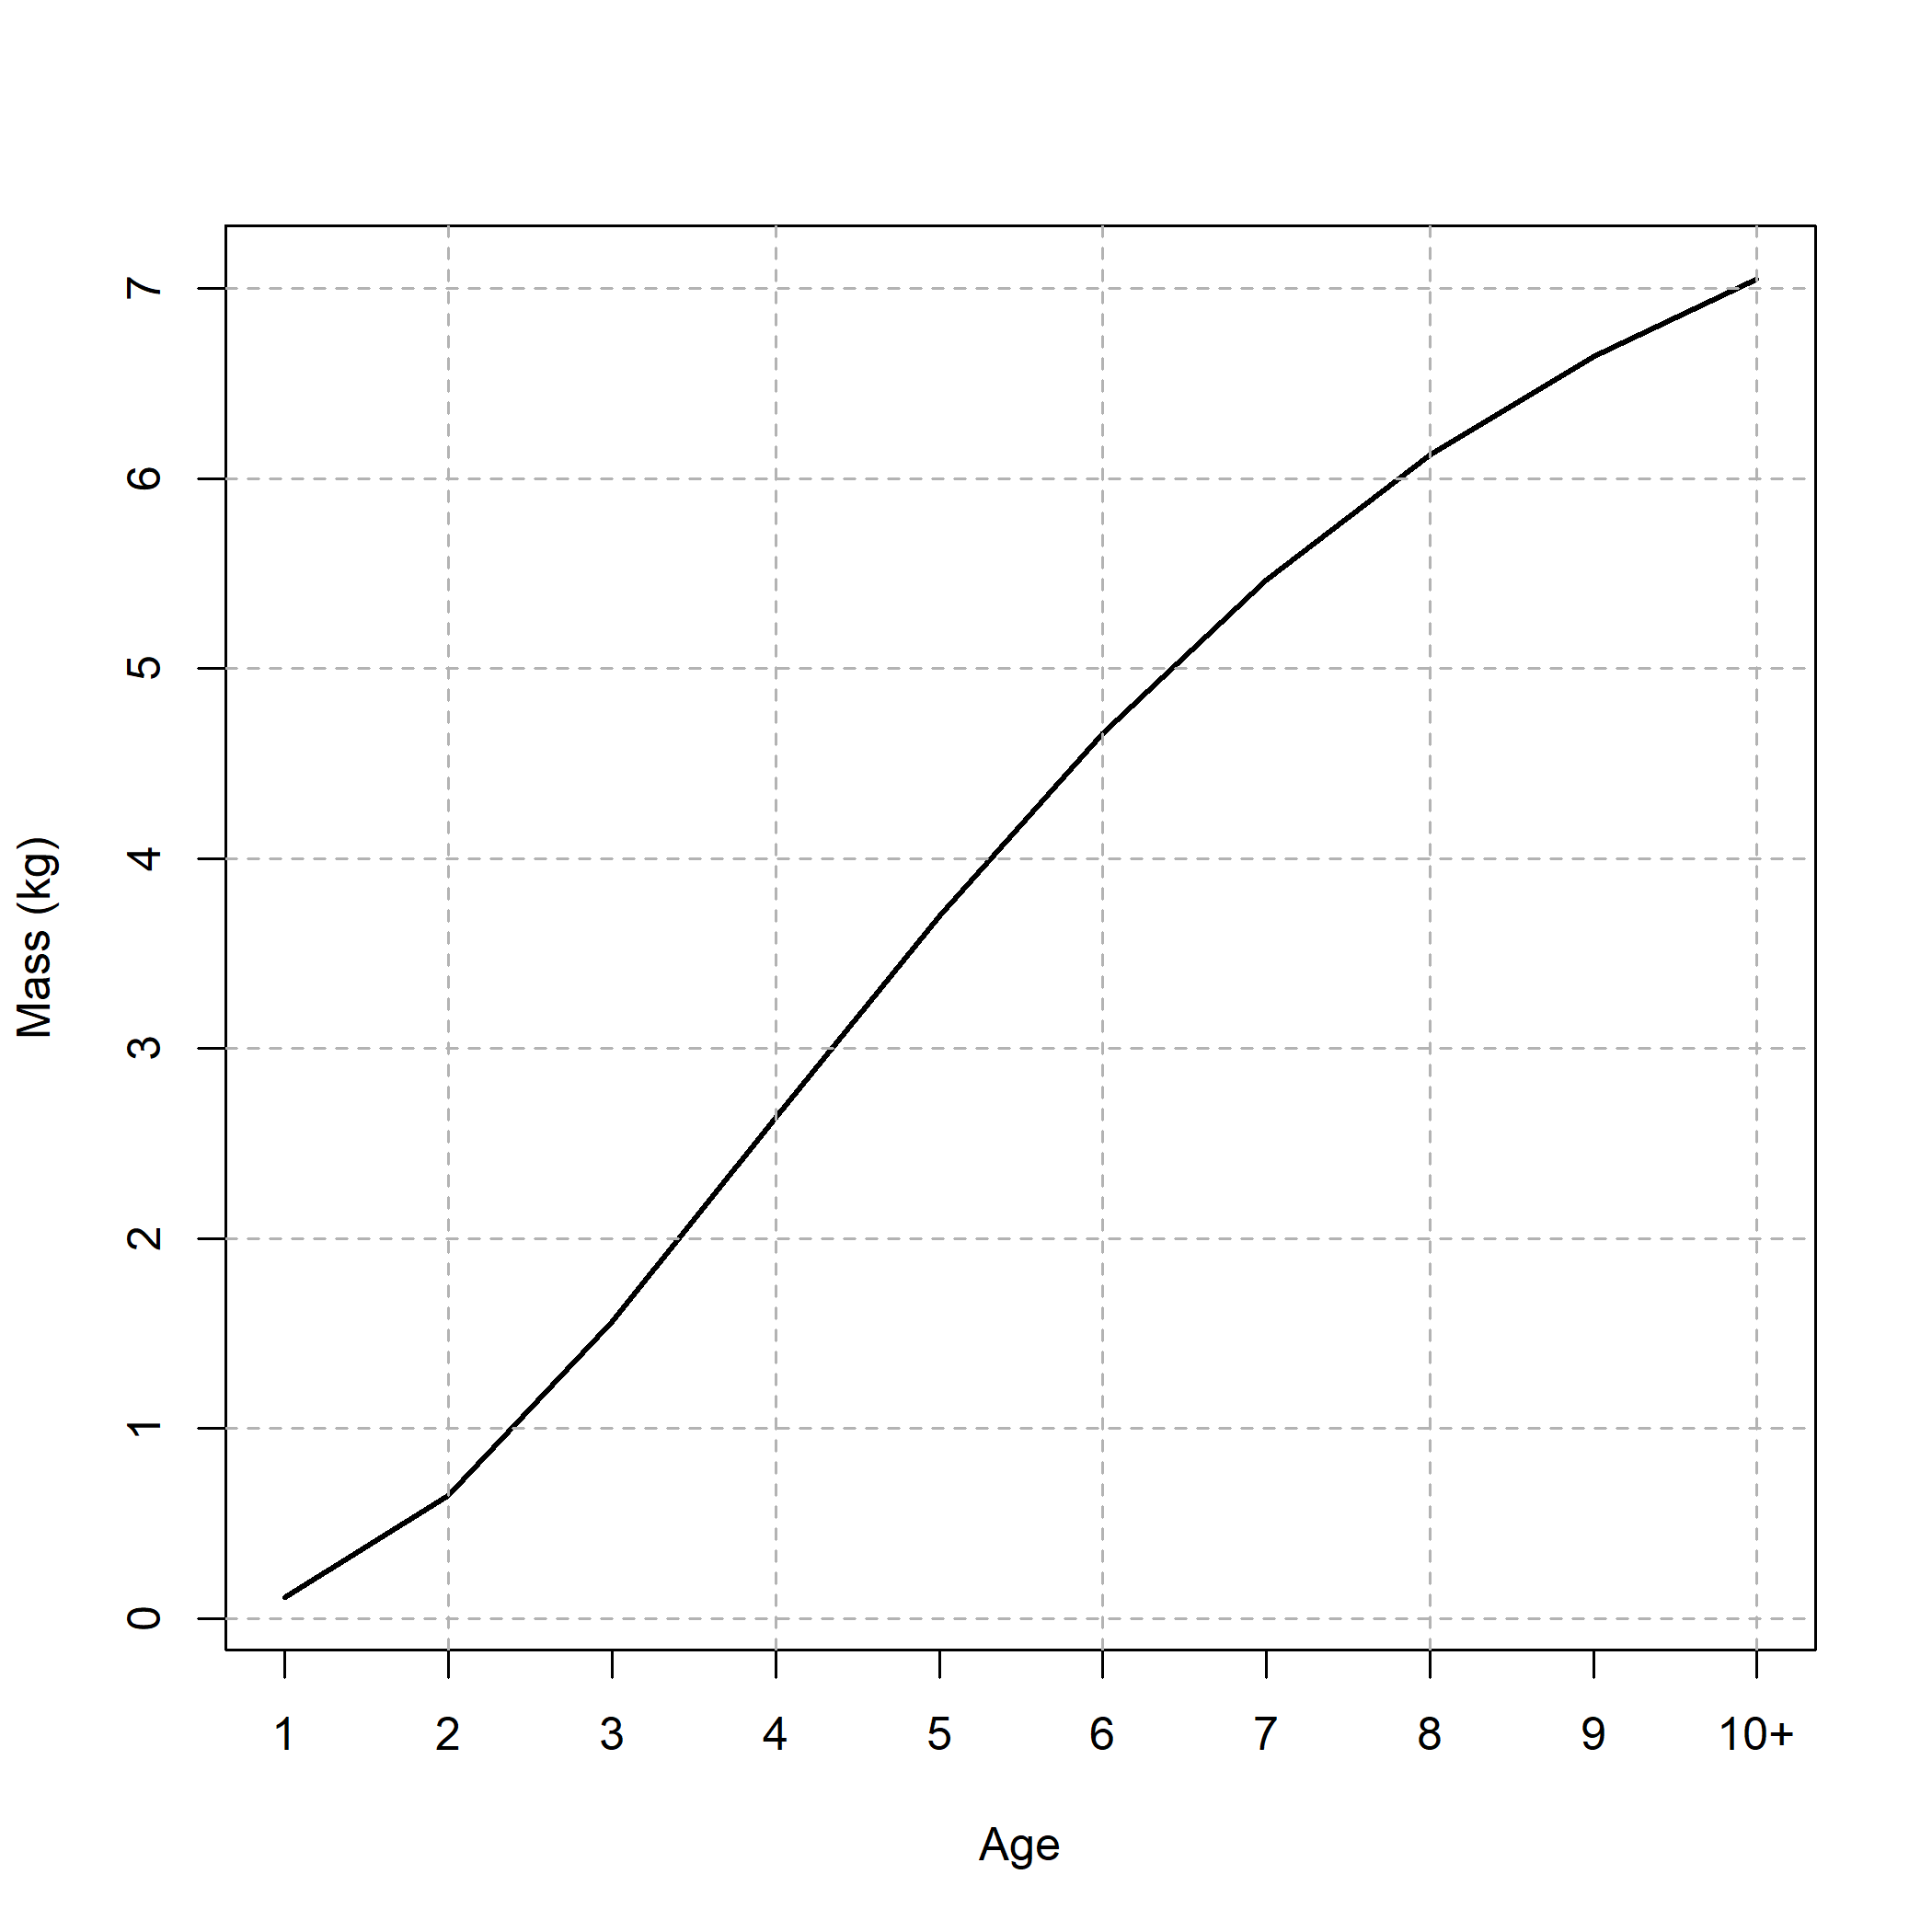
\includegraphics[width = \textwidth]{om_waa.png}
\end{center}
\end{figure}

We assumed a Beverton-Holt stock recruit function with constant
pre-recruit mortality parameters for all operating models. All
post-recruit productivity components are constant in the NAA and survey
catchability process error operating models. Therefore steepness and
unfished recruitment are also constant over the time period for those
operating models \citep{millerbrooks21}. We specified unfished
recruitment = \(R_0 = e^{10}\) and \(\Fmsy = \Fspr[40] = 0.348\) equated
to a steepness of 0.69 and \(\alpha=0.60\) and
\(\beta = 2.4 \times 10^{-5}\) for the \[
N_{1,y} = \frac{\alpha \text{SSB}_{y-1}}{1 + \beta \text{SSB}_{y-1}} 
\] Beverton-Holt parameterization (Figure \ref{om_sr}). For OMs without
process errors on natural mortality we assumed the rate was assumed 0.2.
For OMs with process errors on natural mortality the mean rate was 0.2.

\begin{figure}
\caption{The Beverton-Holt stock recruit relationship assume for all operating models.}\label{om_sr}
\begin{center}
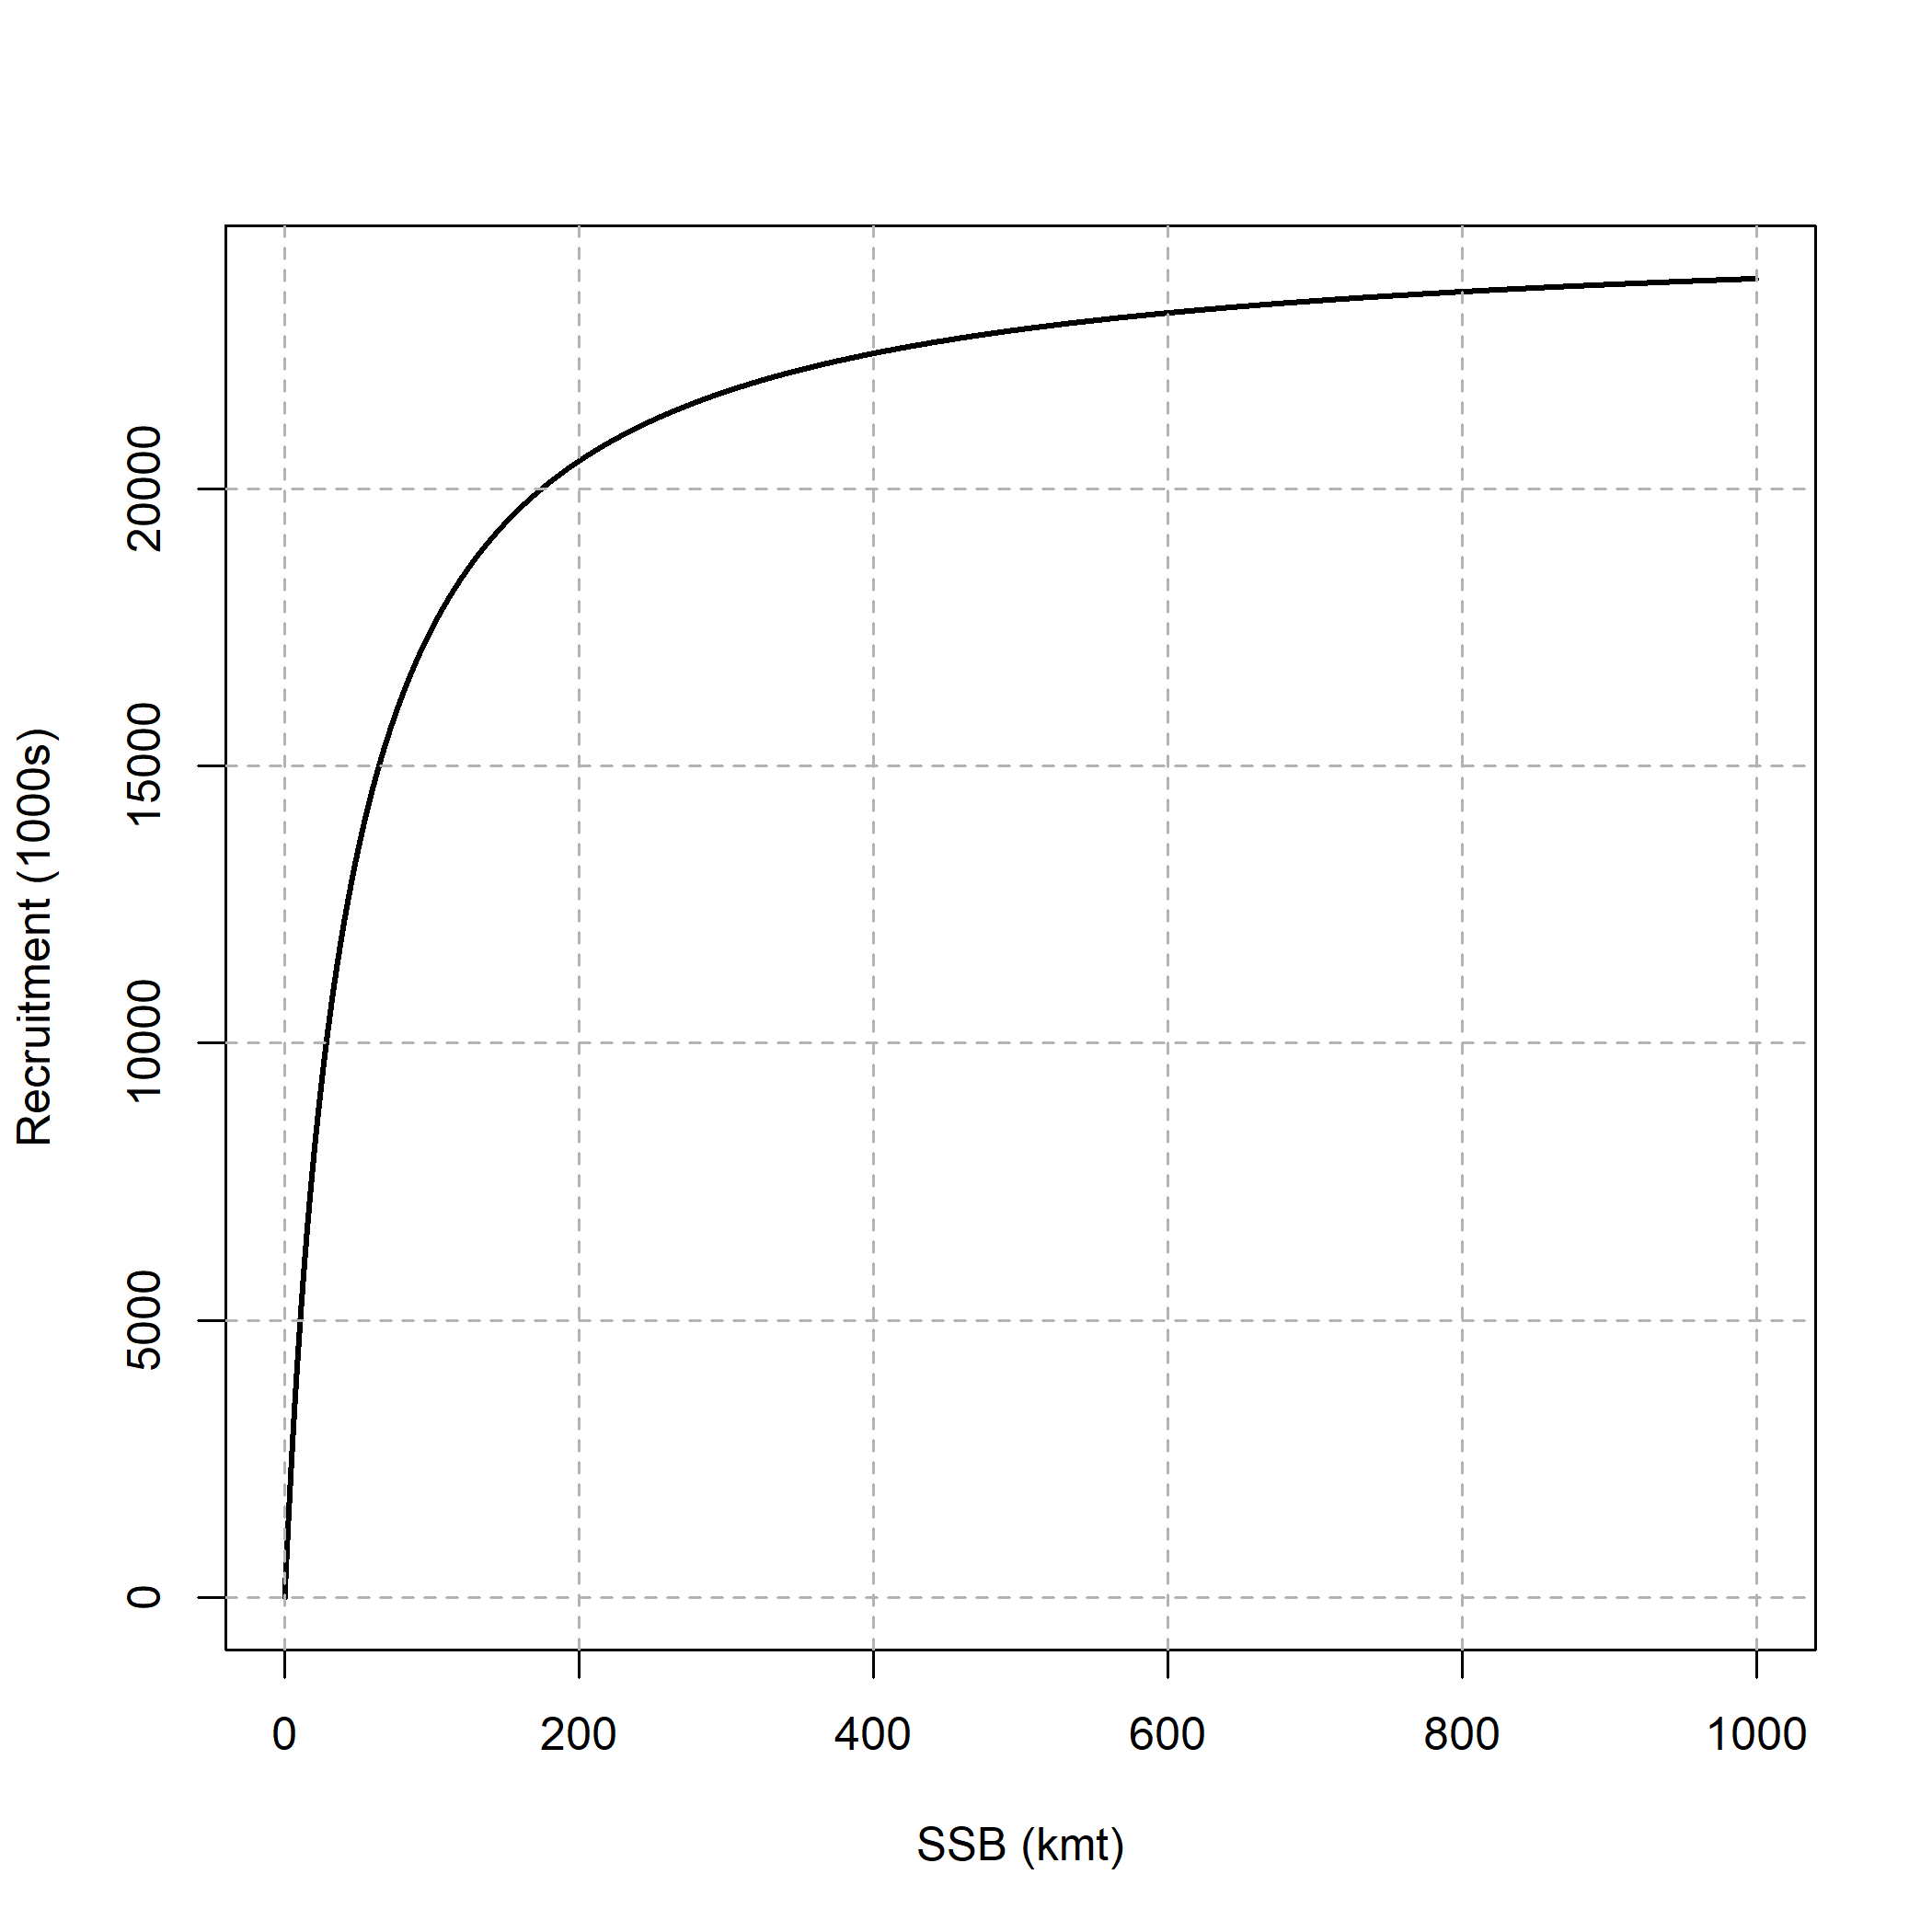
\includegraphics[width = \textwidth]{om_sr.png}
\end{center}
\end{figure}

Two alternative fishing histories were used for operating models. In the
first scenario, the stock experiences overfishing for the first 20 years
and fishing at \Fmsy for the last 20 years. In the second scenario, the
stock is fished at \Fmsy for the entire time period. The magnitude of
the overfishing assumptions is based on average estimates of overfishing
for NE groundfish stocks from \citet{wiedenmannetal19}.
\Citet{legaultetal23} also used similar approaches to defining fishing
mortality histories for operating models.

Initial population was configured at the equilibrium distribution
fishing at either \(F = 2.5\times \Fmsy\) or \(F = \Fmsy\) for the two
alternative fishing histories. That is for a deterministic model, the
age composition would not change over time when the fishing mortality
was constant at the respective level.

For operating models with time-varying random effects for M, steepness
is not constant, but we used the same alpha and beta parameters as other
operating models this equates to a steepness and R0 at the mean of the
time series process for M. For operating models with time-varying random
effects for fishery selectivity, \Fmsy is also not constant however we
use the same F history as other operating models which corresponds to
Fmsy at the mean selectivity parameters.

\hypertarget{fleets}{%
\subsubsection*{Fleets}\label{fleets}}
\addcontentsline{toc}{subsubsection}{Fleets}

We assumed a single fleet operating year round for catch observations
with logistic selectivity for the fleet with \(a_{50} = 5\) and slope =
1 (Figure \ref{om_mean_selectivity}). This selectivity is was used to
define \Fmsy for the Beverton-Holt stock recruitment parameters above.
We assumed a logistic-normal distribution for the age-composition
observations for the fleet.

\begin{figure}
\caption{The selectivity at age assumed for the fishing fleet in operating models without selectivity random effects. The mean selectivity at age across time for the fishing fleet in operating models with selectivity random effects.}\label{om_mean_selectivity}
\begin{center}
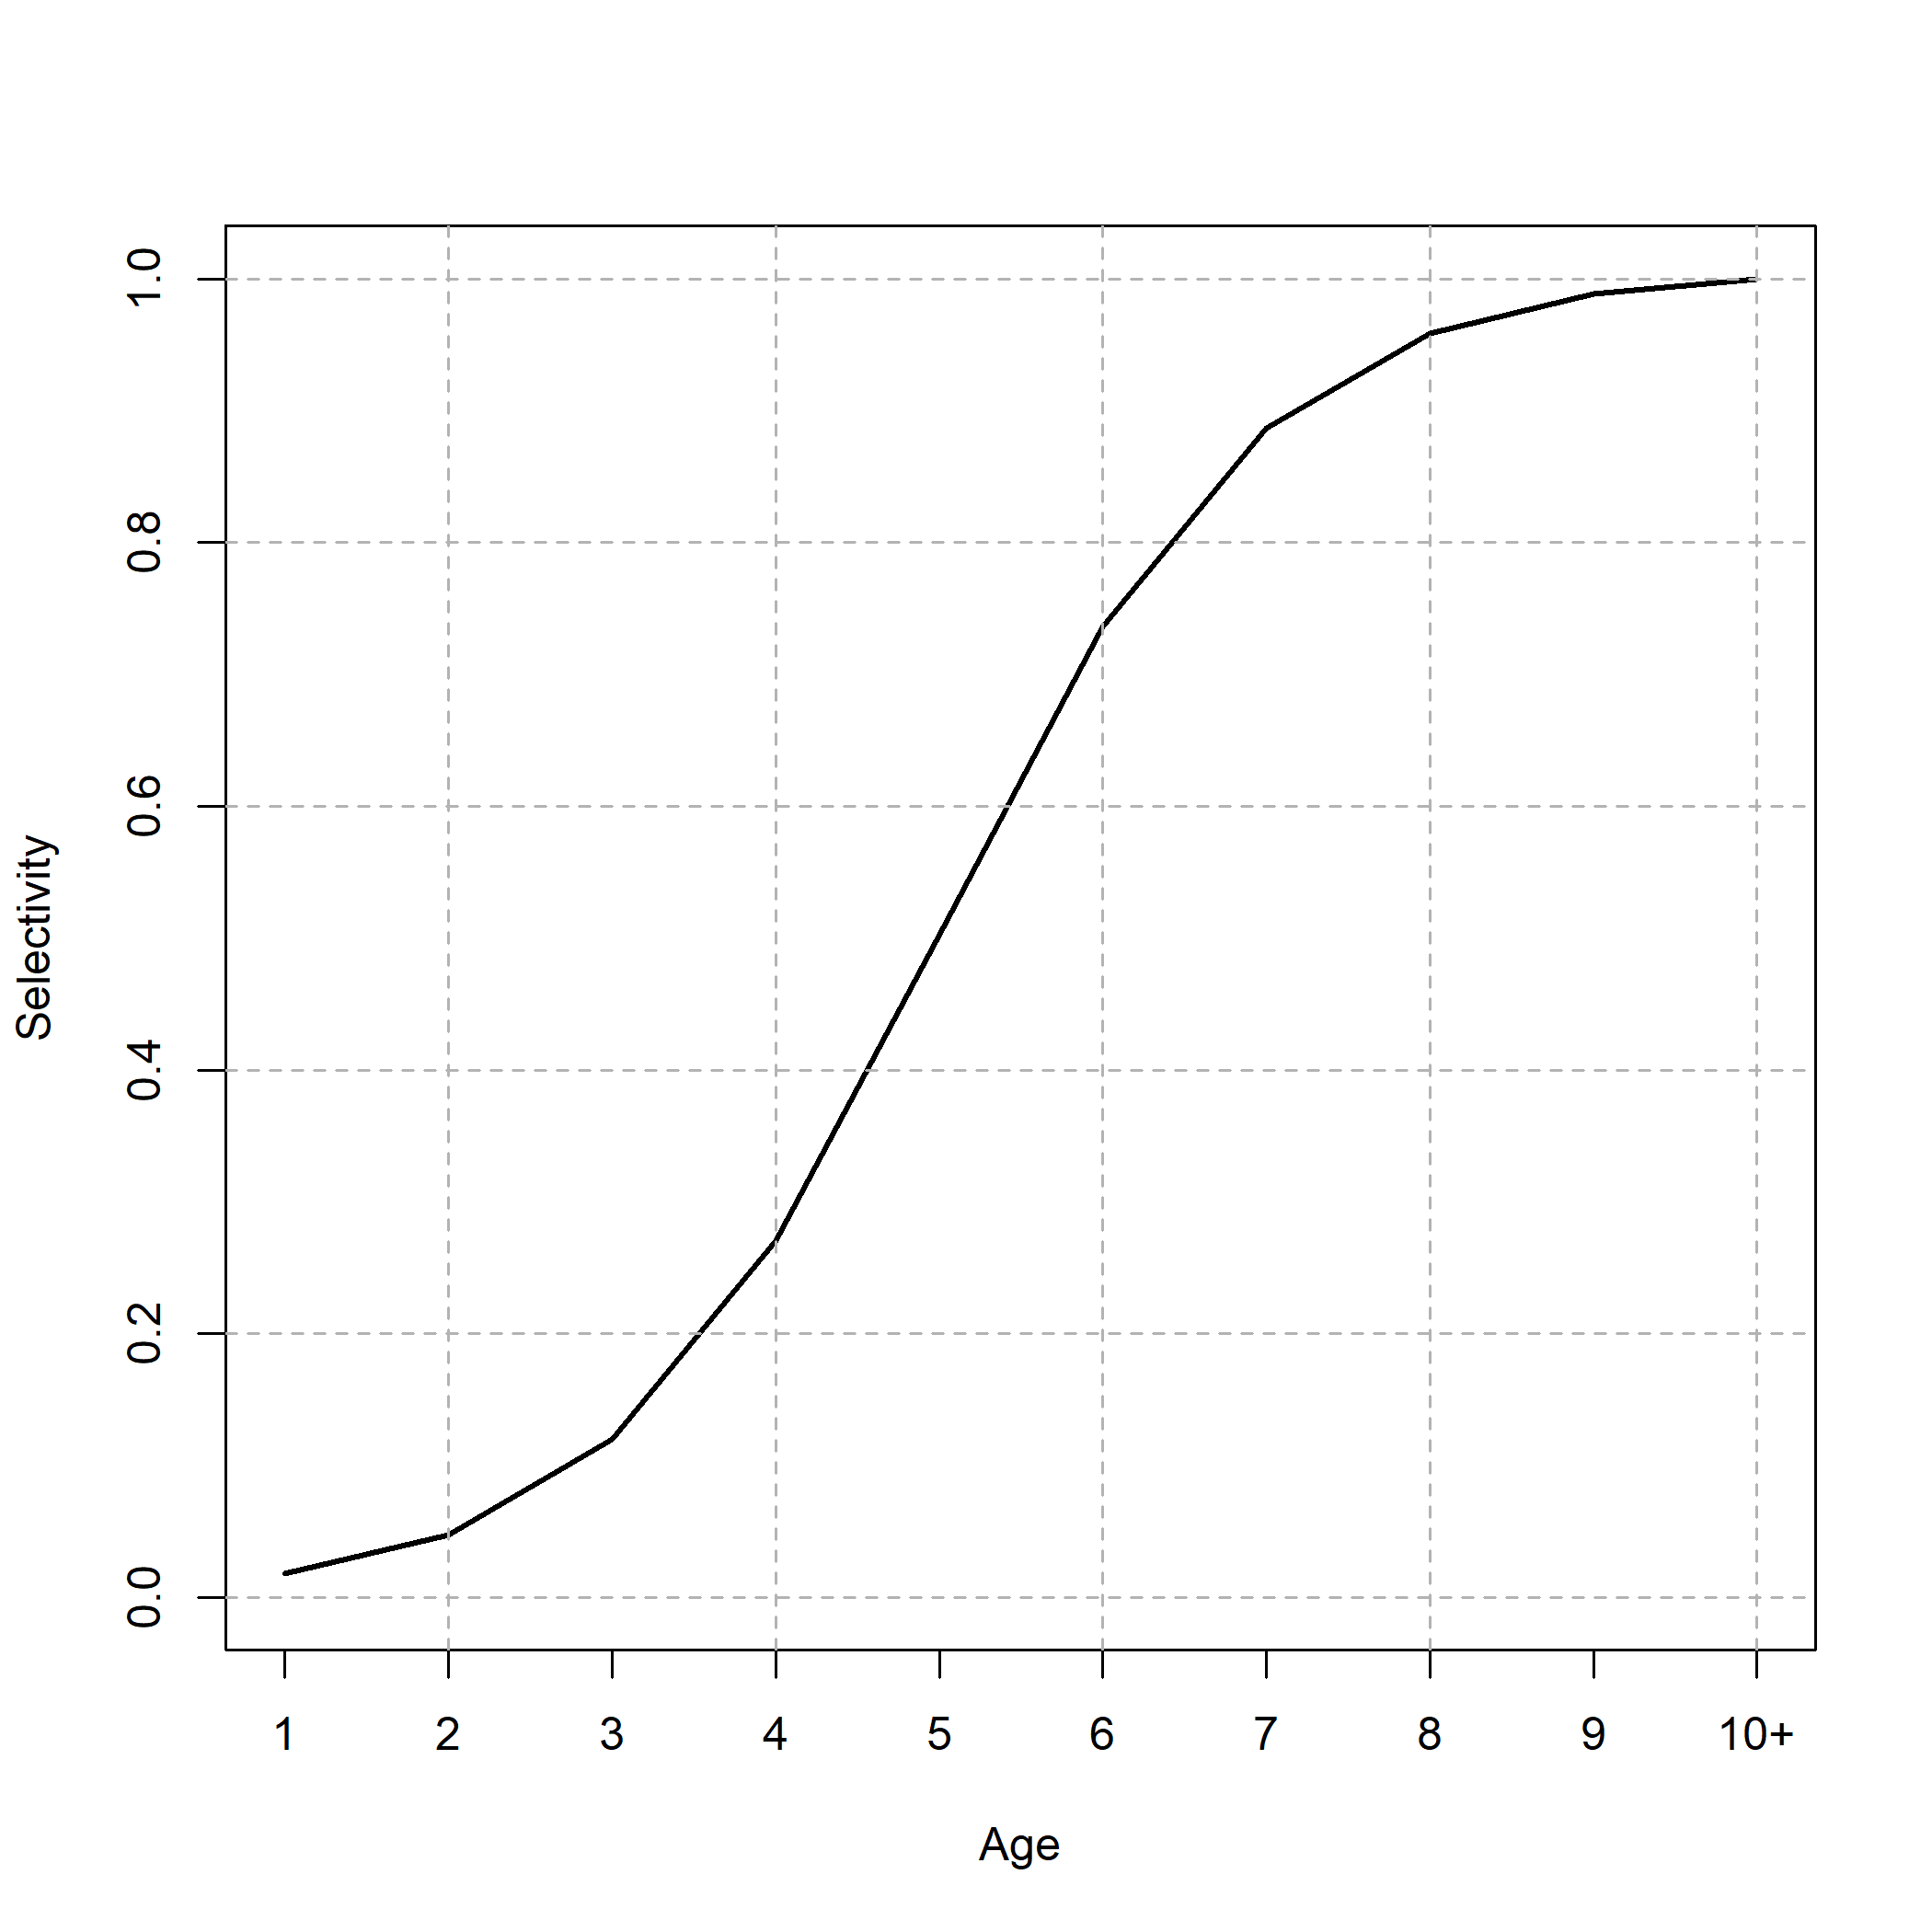
\includegraphics[width = \textwidth]{om_mean_selectivity.png}
\end{center}
\end{figure}

\hypertarget{indices}{%
\subsubsection*{Indices}\label{indices}}
\addcontentsline{toc}{subsubsection}{Indices}

Two time series of surveys are assumed and observed in numbers rather
than biomass for the entire 40 year period with one occurring in the
spring (0.25 way through the year) and one in the fall (0.75 way through
the year). Actually we have it currently configured that both occur 0.5
way through the year. Catchability of both surveys are assumed to be
0.1. Like the fishing fleet, we assumed logistic selectivity for both
indices with \(a_{50} = 5\) and slope = 1 and a logistic-normal
distribution for the age-composition observations.

\hypertarget{observation-uncertainty}{%
\subsubsection*{Observation Uncertainty}\label{observation-uncertainty}}
\addcontentsline{toc}{subsubsection}{Observation Uncertainty}

Standard deviation for log-aggregate catch was 0.1. There were two
levels of observation error variance for indices and age composition for
both indices and fleet catch. A low uncertainty specification assumed
standard deviation of both series of log-aggregate index observations
was 0.1 and the standard deviation of the logistic-normal for age
composition observations was 0.3 In the high uncertainty specification
the standard deviation for log-aggregate indices was 0.4 and that for
the age composition observations was 1.5. For all estimating models,
standard deviation for log-aggregate observations was assumed known
whereas that for the logistic-normal age composition observations was
estimated.

\hypertarget{operating-models-with-random-effects-on-numbers-at-age}{%
\subsubsection*{Operating models with random effects on numbers at
age}\label{operating-models-with-random-effects-on-numbers-at-age}}
\addcontentsline{toc}{subsubsection}{Operating models with random
effects on numbers at age}

The factorial combinations of fishing histories, observation error
assumptions, and marginal variance assumptions for recruitment and
survival results in 24 different operating models with random effects on
recruitment and survival (Table \ref{naa_om_table}).

\begin{landscape}
\begin{table}
\caption{Distinguishing characteristics of the operating models with random effects on survival. Standard deviations (SD) are for log-normal distributed indices and logistic normal distributed age composition observations (fleet and indices). Fishing mortality changes after year 20 (of 40) for fishing histories where fishing mortality is not constant.}\label{naa_om_table}
{\footnotesize \begin{center}
\begin{tabular}{rrrrr}
\hline\hline
\multicolumn{1}{c}{Model}&\multicolumn{1}{c}{$\sigma_R$}&\multicolumn{1}{c}{$\sigma_{2+}$}&\multicolumn{1}{c}{Fishing History}&\multicolumn{1}{c}{Observation Uncertainty}\tabularnewline
\hline
NAA_1&$0.5$&$$&$2.5 F_{\text{MSY}} \rightarrow F_{\text{MSY}}$&Index sigma (log scale) = 0.1, Age composition sigma (logistic normal) = 0.3\tabularnewline
NAA_2&$1.5$&$$&$2.5 F_{\text{MSY}} \rightarrow F_{\text{MSY}}$&Index sigma (log scale) = 0.1, Age composition sigma (logistic normal) = 0.3\tabularnewline
NAA_3&$0.5$&$0.25$&$2.5 F_{\text{MSY}} \rightarrow F_{\text{MSY}}$&Index sigma (log scale) = 0.1, Age composition sigma (logistic normal) = 0.3\tabularnewline
NAA_4&$1.5$&$0.25$&$2.5 F_{\text{MSY}} \rightarrow F_{\text{MSY}}$&Index sigma (log scale) = 0.1, Age composition sigma (logistic normal) = 0.3\tabularnewline
NAA_5&$0.5$&$0.50$&$2.5 F_{\text{MSY}} \rightarrow F_{\text{MSY}}$&Index sigma (log scale) = 0.1, Age composition sigma (logistic normal) = 0.3\tabularnewline
NAA_6&$1.5$&$0.50$&$2.5 F_{\text{MSY}} \rightarrow F_{\text{MSY}}$&Index sigma (log scale) = 0.1, Age composition sigma (logistic normal) = 0.3\tabularnewline
NAA_7&$0.5$&$$&F_{\text{MSY}}&Index sigma (log scale) = 0.1, Age composition sigma (logistic normal) = 0.3\tabularnewline
NAA_8&$1.5$&$$&F_{\text{MSY}}&Index sigma (log scale) = 0.1, Age composition sigma (logistic normal) = 0.3\tabularnewline
NAA_9&$0.5$&$0.25$&F_{\text{MSY}}&Index sigma (log scale) = 0.1, Age composition sigma (logistic normal) = 0.3\tabularnewline
NAA_10&$1.5$&$0.25$&F_{\text{MSY}}&Index sigma (log scale) = 0.1, Age composition sigma (logistic normal) = 0.3\tabularnewline
NAA_11&$0.5$&$0.50$&F_{\text{MSY}}&Index sigma (log scale) = 0.1, Age composition sigma (logistic normal) = 0.3\tabularnewline
NAA_12&$1.5$&$0.50$&F_{\text{MSY}}&Index sigma (log scale) = 0.1, Age composition sigma (logistic normal) = 0.3\tabularnewline
NAA_13&$0.5$&$$&$2.5 F_{\text{MSY}} \rightarrow F_{\text{MSY}}$&Index sigma (log scale) = 0.4, Age composition sigma (logistic normal) = 1.5\tabularnewline
NAA_14&$1.5$&$$&$2.5 F_{\text{MSY}} \rightarrow F_{\text{MSY}}$&Index sigma (log scale) = 0.4, Age composition sigma (logistic normal) = 1.5\tabularnewline
NAA_15&$0.5$&$0.25$&$2.5 F_{\text{MSY}} \rightarrow F_{\text{MSY}}$&Index sigma (log scale) = 0.4, Age composition sigma (logistic normal) = 1.5\tabularnewline
NAA_16&$1.5$&$0.25$&$2.5 F_{\text{MSY}} \rightarrow F_{\text{MSY}}$&Index sigma (log scale) = 0.4, Age composition sigma (logistic normal) = 1.5\tabularnewline
NAA_17&$0.5$&$0.50$&$2.5 F_{\text{MSY}} \rightarrow F_{\text{MSY}}$&Index sigma (log scale) = 0.4, Age composition sigma (logistic normal) = 1.5\tabularnewline
NAA_18&$1.5$&$0.50$&$2.5 F_{\text{MSY}} \rightarrow F_{\text{MSY}}$&Index sigma (log scale) = 0.4, Age composition sigma (logistic normal) = 1.5\tabularnewline
NAA_19&$0.5$&$$&F_{\text{MSY}}&Index sigma (log scale) = 0.4, Age composition sigma (logistic normal) = 1.5\tabularnewline
NAA_20&$1.5$&$$&F_{\text{MSY}}&Index sigma (log scale) = 0.4, Age composition sigma (logistic normal) = 1.5\tabularnewline
NAA_21&$0.5$&$0.25$&F_{\text{MSY}}&Index sigma (log scale) = 0.4, Age composition sigma (logistic normal) = 1.5\tabularnewline
NAA_22&$1.5$&$0.25$&F_{\text{MSY}}&Index sigma (log scale) = 0.4, Age composition sigma (logistic normal) = 1.5\tabularnewline
NAA_23&$0.5$&$0.50$&F_{\text{MSY}}&Index sigma (log scale) = 0.4, Age composition sigma (logistic normal) = 1.5\tabularnewline
NAA_24&$1.5$&$0.50$&F_{\text{MSY}}&Index sigma (log scale) = 0.4, Age composition sigma (logistic normal) = 1.5\tabularnewline
\hline
\end{tabular}\end{center}
}
\end{table}
\end{landscape}

\hypertarget{operating-models-with-random-effects-on-natural-mortality}{%
\subsubsection*{Operating models with random effects on natural
mortality}\label{operating-models-with-random-effects-on-natural-mortality}}
\addcontentsline{toc}{subsubsection}{Operating models with random
effects on natural mortality}

The factorial combinations of fishing histories, observation error
assumptions, and marginal variance and autocorrelation assumptions for
natural mortality results in 16 different operating models with random
effects on natural mortality (Table \ref{M_om_table}). Internally, WHAM
treats natural mortality as a log-transformed parameter \[
\log M_y = \mu_M + \epsilon_{M,y}
\] that is a linear combination of a mean \(\mu_M\) and any annual
random effects marginally distributed as
\(\epsilon_{M,y} \sim \text{N}\left(0,\sigma_M^2\right)\). The values
for the marginal variance and correlation parameters assumed in the
operating models are given in Table \ref{M_om_table}.

\begin{landscape}
\begin{table}
\caption{Distinguishing characteristics of the operating models with random effects on natural mortality. Standard deviations (SD) are for log-normal distributed indices and logistic normal distributed age composition observations (fleet and indices). Fishing mortality changes after year 20 (of 40) for fishing histories where fishing mortality is not constant. For AR1 process errors, $\sigma$ is defined for the marginal distribution of the processes.}\label{M_om_table}
{\begin{center}
\begin{tabular}{rrrrrr}
\hline\hline
\multicolumn{1}{c}{Model}&\multicolumn{1}{c}{$\sigma_R$}&\multicolumn{1}{c}{$\sigma_{M}$}&\multicolumn{1}{c}{$\rho_{M}$}&\multicolumn{1}{c}{Fishing History}&\multicolumn{1}{c}{Observation Uncertainty}\tabularnewline
\hline
$M_{1}$&$0.5$&$0.1$&$0.0$&$2.5 F_{\text{MSY}} \rightarrow F_{\text{MSY}}$&Index SD = 0.1, Age composition SD = 0.3\tabularnewline
$M_{2}$&$0.5$&$0.5$&$0.0$&$2.5 F_{\text{MSY}} \rightarrow F_{\text{MSY}}$&Index SD = 0.1, Age composition SD = 0.3\tabularnewline
$M_{3}$&$0.5$&$0.1$&$0.9$&$2.5 F_{\text{MSY}} \rightarrow F_{\text{MSY}}$&Index SD = 0.1, Age composition SD = 0.3\tabularnewline
$M_{4}$&$0.5$&$0.5$&$0.9$&$2.5 F_{\text{MSY}} \rightarrow F_{\text{MSY}}$&Index SD = 0.1, Age composition SD = 0.3\tabularnewline
$M_{5}$&$0.5$&$0.1$&$0.0$&$F_{\text{MSY}}$&Index SD = 0.1, Age composition SD = 0.3\tabularnewline
$M_{6}$&$0.5$&$0.5$&$0.0$&$F_{\text{MSY}}$&Index SD = 0.1, Age composition SD = 0.3\tabularnewline
$M_{7}$&$0.5$&$0.1$&$0.9$&$F_{\text{MSY}}$&Index SD = 0.1, Age composition SD = 0.3\tabularnewline
$M_{8}$&$0.5$&$0.5$&$0.9$&$F_{\text{MSY}}$&Index SD = 0.1, Age composition SD = 0.3\tabularnewline
$M_{9}$&$0.5$&$0.1$&$0.0$&$2.5 F_{\text{MSY}} \rightarrow F_{\text{MSY}}$&Index SD = 0.4, Age composition SD = 1.5\tabularnewline
$M_{10}$&$0.5$&$0.5$&$0.0$&$2.5 F_{\text{MSY}} \rightarrow F_{\text{MSY}}$&Index SD = 0.4, Age composition SD = 1.5\tabularnewline
$M_{11}$&$0.5$&$0.1$&$0.9$&$2.5 F_{\text{MSY}} \rightarrow F_{\text{MSY}}$&Index SD = 0.4, Age composition SD = 1.5\tabularnewline
$M_{12}$&$0.5$&$0.5$&$0.9$&$2.5 F_{\text{MSY}} \rightarrow F_{\text{MSY}}$&Index SD = 0.4, Age composition SD = 1.5\tabularnewline
$M_{13}$&$0.5$&$0.1$&$0.0$&$F_{\text{MSY}}$&Index SD = 0.4, Age composition SD = 1.5\tabularnewline
$M_{14}$&$0.5$&$0.5$&$0.0$&$F_{\text{MSY}}$&Index SD = 0.4, Age composition SD = 1.5\tabularnewline
$M_{15}$&$0.5$&$0.1$&$0.9$&$F_{\text{MSY}}$&Index SD = 0.4, Age composition SD = 1.5\tabularnewline
$M_{16}$&$0.5$&$0.5$&$0.9$&$F_{\text{MSY}}$&Index SD = 0.4, Age composition SD = 1.5\tabularnewline
\hline
\end{tabular}\end{center}
}
\end{table}
\end{landscape}

\hypertarget{operating-models-with-random-effects-on-fleet-selectivity}{%
\subsubsection*{Operating models with random effects on fleet
selectivity}\label{operating-models-with-random-effects-on-fleet-selectivity}}
\addcontentsline{toc}{subsubsection}{Operating models with random
effects on fleet selectivity}

The factorial combinations of fishing histories, observation error
assumptions, and marginal variance and autocorrelation assumptions for
selectivity parameters results in 16 different operating models with
random effects on selectivity (Table \ref{sel_om_table}). Internally,
WHAM treats selectivity parameter \(s\) as a logit-transformed parameter
\[
\log\left(\frac{p_{s,y}-l_{s}}{u_{s}-p_{s,y}}\right) = \mu_s + \epsilon_{s,y}
\] that is a linear combination of a mean \(\mu_s\) and any annual
random effects marginally distributed as
\(\epsilon_{s,y} \sim \text{N}\left(0,\sigma_s^2\right)\) where the
lower and upper bounds of the parameter (\(l_s\) and \(u_s\)) can be
specified by the user. All selectivity parameters are either \(a_50\) or
slope parameters and we assume bounds of 0 and 10 for all selectivity
parameters for all operating and estimating models. The values for the
marginal variance and correlation parameters assumed in the operating
models are given in Table \ref{sel_om_table}.

\begin{landscape}
\begin{table}
\caption{Distinguishing characteristics of the operating models with random effects on selectivity. Standard deviations (SD) are for log-normal distributed indices and logistic normal distributed age composition observations (fleet and indices). Fishing mortality changes after year 20 (of 40) for fishing histories where fishing mortality is not constant. For AR1 process errors, $\sigma$ is defined for the marginal distribution of the processes.}\label{sel_om_table}
{\begin{center}
\begin{tabular}{rrrrrr}
\hline\hline
\multicolumn{1}{c}{Model}&\multicolumn{1}{c}{$\sigma_R$}&\multicolumn{1}{c}{$\sigma_{\text{Sel}}$}&\multicolumn{1}{c}{$\rho_{\text{Sel}}$}&\multicolumn{1}{c}{Fishing History}&\multicolumn{1}{c}{Observation Uncertainty}\tabularnewline
\hline
$\text{Sel}_{1}$&$0.5$&$0.1$&$0.0$&$2.5 F_{\text{MSY}} \rightarrow F_{\text{MSY}}$&Index SD = 0.1, Age composition SD = 0.3\tabularnewline
$\text{Sel}_{2}$&$0.5$&$0.5$&$0.0$&$2.5 F_{\text{MSY}} \rightarrow F_{\text{MSY}}$&Index SD = 0.1, Age composition SD = 0.3\tabularnewline
$\text{Sel}_{3}$&$0.5$&$0.1$&$0.9$&$2.5 F_{\text{MSY}} \rightarrow F_{\text{MSY}}$&Index SD = 0.1, Age composition SD = 0.3\tabularnewline
$\text{Sel}_{4}$&$0.5$&$0.5$&$0.9$&$2.5 F_{\text{MSY}} \rightarrow F_{\text{MSY}}$&Index SD = 0.1, Age composition SD = 0.3\tabularnewline
$\text{Sel}_{5}$&$0.5$&$0.1$&$0.0$&$F_{\text{MSY}}$&Index SD = 0.1, Age composition SD = 0.3\tabularnewline
$\text{Sel}_{6}$&$0.5$&$0.5$&$0.0$&$F_{\text{MSY}}$&Index SD = 0.1, Age composition SD = 0.3\tabularnewline
$\text{Sel}_{7}$&$0.5$&$0.1$&$0.9$&$F_{\text{MSY}}$&Index SD = 0.1, Age composition SD = 0.3\tabularnewline
$\text{Sel}_{8}$&$0.5$&$0.5$&$0.9$&$F_{\text{MSY}}$&Index SD = 0.1, Age composition SD = 0.3\tabularnewline
$\text{Sel}_{9}$&$0.5$&$0.1$&$0.0$&$2.5 F_{\text{MSY}} \rightarrow F_{\text{MSY}}$&Index SD = 0.4, Age composition SD = 1.5\tabularnewline
$\text{Sel}_{10}$&$0.5$&$0.5$&$0.0$&$2.5 F_{\text{MSY}} \rightarrow F_{\text{MSY}}$&Index SD = 0.4, Age composition SD = 1.5\tabularnewline
$\text{Sel}_{11}$&$0.5$&$0.1$&$0.9$&$2.5 F_{\text{MSY}} \rightarrow F_{\text{MSY}}$&Index SD = 0.4, Age composition SD = 1.5\tabularnewline
$\text{Sel}_{12}$&$0.5$&$0.5$&$0.9$&$2.5 F_{\text{MSY}} \rightarrow F_{\text{MSY}}$&Index SD = 0.4, Age composition SD = 1.5\tabularnewline
$\text{Sel}_{13}$&$0.5$&$0.1$&$0.0$&$F_{\text{MSY}}$&Index SD = 0.4, Age composition SD = 1.5\tabularnewline
$\text{Sel}_{14}$&$0.5$&$0.5$&$0.0$&$F_{\text{MSY}}$&Index SD = 0.4, Age composition SD = 1.5\tabularnewline
$\text{Sel}_{15}$&$0.5$&$0.1$&$0.9$&$F_{\text{MSY}}$&Index SD = 0.4, Age composition SD = 1.5\tabularnewline
$\text{Sel}_{16}$&$0.5$&$0.5$&$0.9$&$F_{\text{MSY}}$&Index SD = 0.4, Age composition SD = 1.5\tabularnewline
\hline
\end{tabular}\end{center}
}
\end{table}
\end{landscape}

\hypertarget{operating-models-with-random-effects-on-index-catchability}{%
\subsubsection*{Operating models with random effects on index
catchability}\label{operating-models-with-random-effects-on-index-catchability}}
\addcontentsline{toc}{subsubsection}{Operating models with random
effects on index catchability}

The factorial combinations of fishing histories, observation error
assumptions, and marginal variance and autocorrelation assumptions for
catchability results in 16 different operating models with random
effects on catchability (Table \ref{q_om_table}). Internally, WHAM
treats catchability for index \(i\) as a logit-transformed parameter \[
\log\left(\frac{q_{i,y}-l_{i}}{u_{i}-q_{i,y}}\right) = \mu_i + \epsilon_{i,y}
\] that is a linear combination of a mean \(\mu_i\) and any annual
random effects marginally distributed as
\(\epsilon_{i,y} \sim \text{N}\left(0,\sigma_i^2\right)\) where the
lower and upper bounds of the catchability (\(l_i\) and \(u_i\)) can be
specified by the user. Here we assume bounds of 0 and 1000 for all
operating and estimating models. For operating and estimation models
with process errors on catchability, the temporal variation is only
assumed for the first index. The values for the marginal variance and
correlation parameters assumed in the operating models are given in
Table \ref{q_om_table}

\begin{landscape}
\begin{table}
\caption{Distinguishing characteristics of the operating models with random effects on catchability. Standard deviations (SD) are for log-normal distributed indices and logistic normal distributed age composition observations (fleet and indices). Fishing mortality changes after year 20 (of 40) for fishing histories where fishing mortality is not constant. For AR1 process errors, $\sigma$ is defined for the marginal distribution of the processes.}\label{q_om_table}
{\begin{center}
\begin{tabular}{rrrrrr}
\hline\hline
\multicolumn{1}{c}{Model}&\multicolumn{1}{c}{$\sigma_R$}&\multicolumn{1}{c}{$\sigma_{q}$}&\multicolumn{1}{c}{$\rho_{q}$}&\multicolumn{1}{c}{Fishing History}&\multicolumn{1}{c}{Observation Uncertainty}\tabularnewline
\hline
$q_{1}$&$0.5$&$0.1$&$0.0$&$2.5 F_{\text{MSY}} \rightarrow F_{\text{MSY}}$&Index SD = 0.1, Age composition SD = 0.3\tabularnewline
$q_{2}$&$0.5$&$0.5$&$0.0$&$2.5 F_{\text{MSY}} \rightarrow F_{\text{MSY}}$&Index SD = 0.1, Age composition SD = 0.3\tabularnewline
$q_{3}$&$0.5$&$0.1$&$0.9$&$2.5 F_{\text{MSY}} \rightarrow F_{\text{MSY}}$&Index SD = 0.1, Age composition SD = 0.3\tabularnewline
$q_{4}$&$0.5$&$0.5$&$0.9$&$2.5 F_{\text{MSY}} \rightarrow F_{\text{MSY}}$&Index SD = 0.1, Age composition SD = 0.3\tabularnewline
$q_{5}$&$0.5$&$0.1$&$0.0$&$F_{\text{MSY}}$&Index SD = 0.1, Age composition SD = 0.3\tabularnewline
$q_{6}$&$0.5$&$0.5$&$0.0$&$F_{\text{MSY}}$&Index SD = 0.1, Age composition SD = 0.3\tabularnewline
$q_{7}$&$0.5$&$0.1$&$0.9$&$F_{\text{MSY}}$&Index SD = 0.1, Age composition SD = 0.3\tabularnewline
$q_{8}$&$0.5$&$0.5$&$0.9$&$F_{\text{MSY}}$&Index SD = 0.1, Age composition SD = 0.3\tabularnewline
$q_{9}$&$0.5$&$0.1$&$0.0$&$2.5 F_{\text{MSY}} \rightarrow F_{\text{MSY}}$&Index SD = 0.4, Age composition SD = 1.5\tabularnewline
$q_{10}$&$0.5$&$0.5$&$0.0$&$2.5 F_{\text{MSY}} \rightarrow F_{\text{MSY}}$&Index SD = 0.4, Age composition SD = 1.5\tabularnewline
$q_{11}$&$0.5$&$0.1$&$0.9$&$2.5 F_{\text{MSY}} \rightarrow F_{\text{MSY}}$&Index SD = 0.4, Age composition SD = 1.5\tabularnewline
$q_{12}$&$0.5$&$0.5$&$0.9$&$2.5 F_{\text{MSY}} \rightarrow F_{\text{MSY}}$&Index SD = 0.4, Age composition SD = 1.5\tabularnewline
$q_{13}$&$0.5$&$0.1$&$0.0$&$F_{\text{MSY}}$&Index SD = 0.4, Age composition SD = 1.5\tabularnewline
$q_{14}$&$0.5$&$0.5$&$0.0$&$F_{\text{MSY}}$&Index SD = 0.4, Age composition SD = 1.5\tabularnewline
$q_{15}$&$0.5$&$0.1$&$0.9$&$F_{\text{MSY}}$&Index SD = 0.4, Age composition SD = 1.5\tabularnewline
$q_{16}$&$0.5$&$0.5$&$0.9$&$F_{\text{MSY}}$&Index SD = 0.4, Age composition SD = 1.5\tabularnewline
\hline
\end{tabular}\end{center}
}
\end{table}
\end{landscape}

\hypertarget{estimating-models}{%
\subsection*{Estimating models}\label{estimating-models}}
\addcontentsline{toc}{subsection}{Estimating models}

For each data set simulated from an operating model 20 estimating models
were fit. A total of 32 different estimating models were fit across all
operating models where the subset of 20 depended on the source of
process error (Table \ref{em_table}). The first 20 estimating models in
Table \ref{em_table} were fit to simulate data sets from R and R+S
operating models. Estimating models 5 to 24 in Table \ref{em_table} were
fit to simulate data sets from R+M operating models. Estimating models 5
to 20 and 25-28 in Table \ref{em_table} were fit to simulate data sets
from R+Sel operating models. Finally, estimating models 5 to 20 and
29-32 in Table \ref{em_table} were fit to simulate data sets from R+q
operating models.

\begin{table}
\caption{Distinguishing characteristics of the estimating models.}\label{em_table}
{\scriptsize \begin{center}
\begin{tabular}{rrrr}
\hline\hline
\multicolumn{1}{c}{Model}&\multicolumn{1}{c}{Recruitment model}&\multicolumn{1}{c}{Mean $M$}&\multicolumn{1}{c}{Process error assumption}\tabularnewline
\hline
EM$_{1}$&Mean recruitment&0.2&Recruitment ($\sigma_R$ estimated)\tabularnewline
EM$_{2}$&Beverton-Holt&0.2&Recruitment ($\sigma_R$ estimated)\tabularnewline
EM$_{3}$&Mean recruitment&Estimated&Recruitment ($\sigma_R$ estimated)\tabularnewline
EM$_{4}$&Beverton-Holt&Estimated&Recruitment ($\sigma_R$ estimated)\tabularnewline
EM$_{5}$&Mean recruitment&0.2&Recruitment and survival ($\sigma_R$, $\sigma_{2+}$ estimated)\tabularnewline
EM$_{6}$&Beverton-Holt&0.2&Recruitment and survival ($\sigma_R$, $\sigma_{2+}$ estimated)\tabularnewline
EM$_{7}$&Mean recruitment&Estimated&Recruitment and survival ($\sigma_R$, $\sigma_{2+}$ estimated)\tabularnewline
EM$_{8}$&Beverton-Holt&Estimated&Recruitment and survival ($\sigma_R$, $\sigma_{2+}$ estimated)\tabularnewline
EM$_{9}$&Mean recruitment&0.2&Recruitment and uncorrelated natural mortality ($\sigma_R$, $\sigma_{M}$ estimated, $\rho_{M} = 0$)\tabularnewline
EM$_{10}$&Beverton-Holt&0.2&Recruitment and uncorrelated natural mortality ($\sigma_R$, $\sigma_{M}$ estimated, $\rho_{M} = 0$)\tabularnewline
EM$_{11}$&Mean recruitment&Estimated&Recruitment and uncorrelated natural mortality ($\sigma_R$, $\sigma_{M}$ estimated, $\rho_{M} = 0$)\tabularnewline
EM$_{12}$&Beverton-Holt&Estimated&Recruitment and uncorrelated natural mortality ($\sigma_R$, $\sigma_{M}$ estimated, $\rho_{M} = 0$)\tabularnewline
EM$_{13}$&Mean recruitment&0.2&Recruitment and uncorrelated fleet selectivity ($\sigma_R$, $\sigma_{\text{Sel}}$ estimated, $\rho_{\text{Sel}} = 0$)\tabularnewline
EM$_{14}$&Beverton-Holt&0.2&Recruitment and uncorrelated fleet selectivity ($\sigma_R$, $\sigma_{\text{Sel}}$ estimated, $\rho_{\text{Sel}} = 0$)\tabularnewline
EM$_{15}$&Mean recruitment&Estimated&Recruitment and uncorrelated fleet selectivity ($\sigma_R$, $\sigma_{\text{Sel}}$ estimated, $\rho_{\text{Sel}} = 0$)\tabularnewline
EM$_{16}$&Beverton-Holt&Estimated&Recruitment and uncorrelated fleet selectivity ($\sigma_R$, $\sigma_{\text{Sel}}$ estimated, $\rho_{\text{Sel}} = 0$)\tabularnewline
EM$_{17}$&Mean recruitment&0.2&Recruitment and uncorrelated catchability (spring index) ($\sigma_R$, $\sigma_{q}$ estimated, $\rho_{q} = 0$)\tabularnewline
EM$_{18}$&Beverton-Holt&0.2&Recruitment and uncorrelated catchability (spring index) ($\sigma_R$, $\sigma_{q}$ estimated, $\rho_{q} = 0$)\tabularnewline
EM$_{19}$&Mean recruitment&Estimated&Recruitment and uncorrelated catchability (spring index) ($\sigma_R$, $\sigma_{q}$ estimated, $\rho_{q} = 0$)\tabularnewline
EM$_{20}$&Beverton-Holt&Estimated&Recruitment and uncorrelated catchability (spring index) ($\sigma_R$, $\sigma_{q}$ estimated, $\rho_{q} = 0$)\tabularnewline
EM$_{21}$&Mean recruitment&0.2&Recruitment and AR1 natural mortality ($\sigma_R$, $\sigma_{M}$, $\rho_{M}$ estimated)\tabularnewline
EM$_{22}$&Beverton-Holt&0.2&Recruitment and AR1 natural mortality ($\sigma_R$, $\sigma_{M}$, $\rho_{M}$ estimated)\tabularnewline
EM$_{23}$&Mean recruitment&Estimated&Recruitment and AR1 natural mortality ($\sigma_R$, $\sigma_{M}$, $\rho_{M}$ estimated)\tabularnewline
EM$_{24}$&Beverton-Holt&Estimated&Recruitment and AR1 natural mortality ($\sigma_R$, $\sigma_{M}$, $\rho_{M}$ estimated)\tabularnewline
EM$_{25}$&Mean recruitment&0.2&Recruitment and AR1 selectivity ($\sigma_R$, $\sigma_{\text{Sel}}$, $\rho_{\text{Sel}}$ estimated)\tabularnewline
EM$_{26}$&Beverton-Holt&0.2&Recruitment and AR1 selectivity ($\sigma_R$, $\sigma_{\text{Sel}}$, $\rho_{\text{Sel}}$ estimated)\tabularnewline
EM$_{27}$&Mean recruitment&Estimated&Recruitment and AR1 selectivity ($\sigma_R$, $\sigma_{\text{Sel}}$, $\rho_{\text{Sel}}$ estimated)\tabularnewline
EM$_{28}$&Beverton-Holt&Estimated&Recruitment and AR1 selectivity ($\sigma_R$, $\sigma_{\text{Sel}}$, $\rho_{\text{Sel}}$ estimated)\tabularnewline
EM$_{29}$&Mean recruitment&0.2&Recruitment and AR1 catchability (spring index) ($\sigma_R$, $\sigma_{q}$, $\rho_{q}$ estimated)\tabularnewline
EM$_{30}$&Beverton-Holt&0.2&Recruitment and AR1 catchability (spring index) ($\sigma_R$, $\sigma_{q}$, $\rho_{q}$ estimated)\tabularnewline
EM$_{31}$&Mean recruitment&Estimated&Recruitment and AR1 catchability (spring index) ($\sigma_R$, $\sigma_{q}$, $\rho_{q}$ estimated)\tabularnewline
EM$_{32}$&Beverton-Holt&Estimated&Recruitment and AR1 catchability (spring index) ($\sigma_R$, $\sigma_{q}$, $\rho_{q}$ estimated)\tabularnewline
\hline
\end{tabular}\end{center}
}
\end{table}

SR estimation or not

Initial values for BH parameters are the true values. Initial values for
mean R model = true R0.

M estimation or not

NAA\_re Random effects on Recruitment only or random effects on
recruitment and transitions among older numbers at age.

M\_re Random effects on Recruitment only, M constant across age .

sel\_re Random effects on Recruitment only, fleet logistic selectivity
RE model?

q\_re Random effects on Recruitment only, one survey catchability RE
model?

Simulations were all carried out on the University of Massachusetts
Green High-Performance Computing Cluster. Code for completing the
simulations and summarization of results can be found at
github.com/timjmiller/SSRTWG/Project\_0. We used the wham package
version 1.X.X (commit 77bbd94).

\hypertarget{measures-of-reliability}{%
\subsection*{Measures of reliability}\label{measures-of-reliability}}
\addcontentsline{toc}{subsection}{Measures of reliability}

The first measure of reliability we investigated was frequency of
convergence when fitting each estimating model to the simulated data
sets. There are various ways to assess convergence of the fit. We
summarized 5 alternative categories of convergence. 1. Did the
optimization routine (stats::nlminb) complete without error? 2. Did the
stats::nlminb convergence flag = 0 indicate successful convergence? 3.
Was the maximum absolute value of the gradient of the log-likelihood
\textless{} \(1\times10^{-6}\)? 4. Did TMB::sdreport provide non-NA
values for all fixed effects standard errors? 5. Did TMB::sdreport
provide all standard errors \textless{} 100?

The first convergence criterion assesses whether the model crashes. The
third is a measure that assesses how flat the likelihood is at the
optimized point of the likelihood surface. The fourth and fifth criteria
are specific to the hessian-based standard error reporting provided by
TMB. the TMB::sdreport function will sometimes return standard error
estimates even when the calculated hessian is not invertible (fourth
criterion). It will also provide large standard errors for some
parameters that are not estimated well or are near bounds on the
transformed scale that is of primary interest. For example, variance
parameters for random effects can often be estimated near 0 when the fit
suggests no variation in the random effects or, equivalently, that the
model without random effects is better.

\hypertarget{aic-for-model-selection}{%
\subsubsection*{AIC for model selection}\label{aic-for-model-selection}}
\addcontentsline{toc}{subsubsection}{AIC for model selection}

We measured the frequency of correct model selection using marginal AIC.
For a given operating model we the set of models that were considered
all made the same assumptions on whether or not to estimate M and
whether a stock-recruit function is assumed.

We also measured the frequency of correctly selecting models with
Beverton-Holt stock recruit function assumed over models without the
stock-recruit function (null model). Because the proportions of
simulations where the correct model was chosen for a given set of
operating model factors implied generally poor performance of AIC, we
analyzed the effect of variation in SSB on the probability of lower AIC
of the BH models. We fit binomial generalize linear models to the
observed AIC choice for each data set as a function of log(SD(SSB)) and
operating model.

\hypertarget{bias}{%
\subsubsection*{Bias}\label{bias}}
\addcontentsline{toc}{subsubsection}{Bias}

We estimated relative bias \[
\widehat {\text{RB}}\left(\theta\right) = \frac{1}{N} \sum^N_{i = 1} \frac{\widehat \theta_i - \theta_i}{\theta_i}
\] of annual SSB and fully-selected fishing mortality for each
estimation model and constructed 95\% confidence intervals for the
median relative bias using the binomial distribution approach as in
\citet{stockmiller21}. We also estimated bias of stock-recruit
parameters for estimation models that assumed the Beverton-Holt stock
recruit function.

\hypertarget{mohns-rho}{%
\subsubsection*{Mohn's rho}\label{mohns-rho}}
\addcontentsline{toc}{subsubsection}{Mohn's rho}

We estimated Mohn's rho for SSB, fully-selected fishing mortality, and
recruitment for each estimation model. We estimated 7 peels for each
estimation model. We calculated median 95\% confidence intervals for
Mohn's rho using the same methods as that for bias.

\hypertarget{results}{%
\section*{Results}\label{results}}
\addcontentsline{toc}{section}{Results}

\hypertarget{convergence-performance}{%
\subsection*{Convergence performance}\label{convergence-performance}}
\addcontentsline{toc}{subsection}{Convergence performance}

Probability of convergence was better for models that assumed the
correct source of process error, assumed M was known, and did not assume
stock-recruit relationships.

\hypertarget{r-rs-operating-models}{%
\subsubsection*{R, R+S operating models}\label{r-rs-operating-models}}
\addcontentsline{toc}{subsubsection}{R, R+S operating models}

Figures \ref{naa_om_em_R_MF_convergence} to
\ref{naa_om_em_BH_ME_convergence}

\begin{landscape}
\begin{figure}
\caption{Probability of each type of convergence of estimating models with alternative process error assumptions for operating models that have process error structures R and R+S. vertical lines represent 95\% confidence intervals. All estimating models estimate mean recruitment rather than a stock-recruit relationship and and M is fixed at the true value.}\label{naa_om_em_R_MF_convergence}
\begin{center}
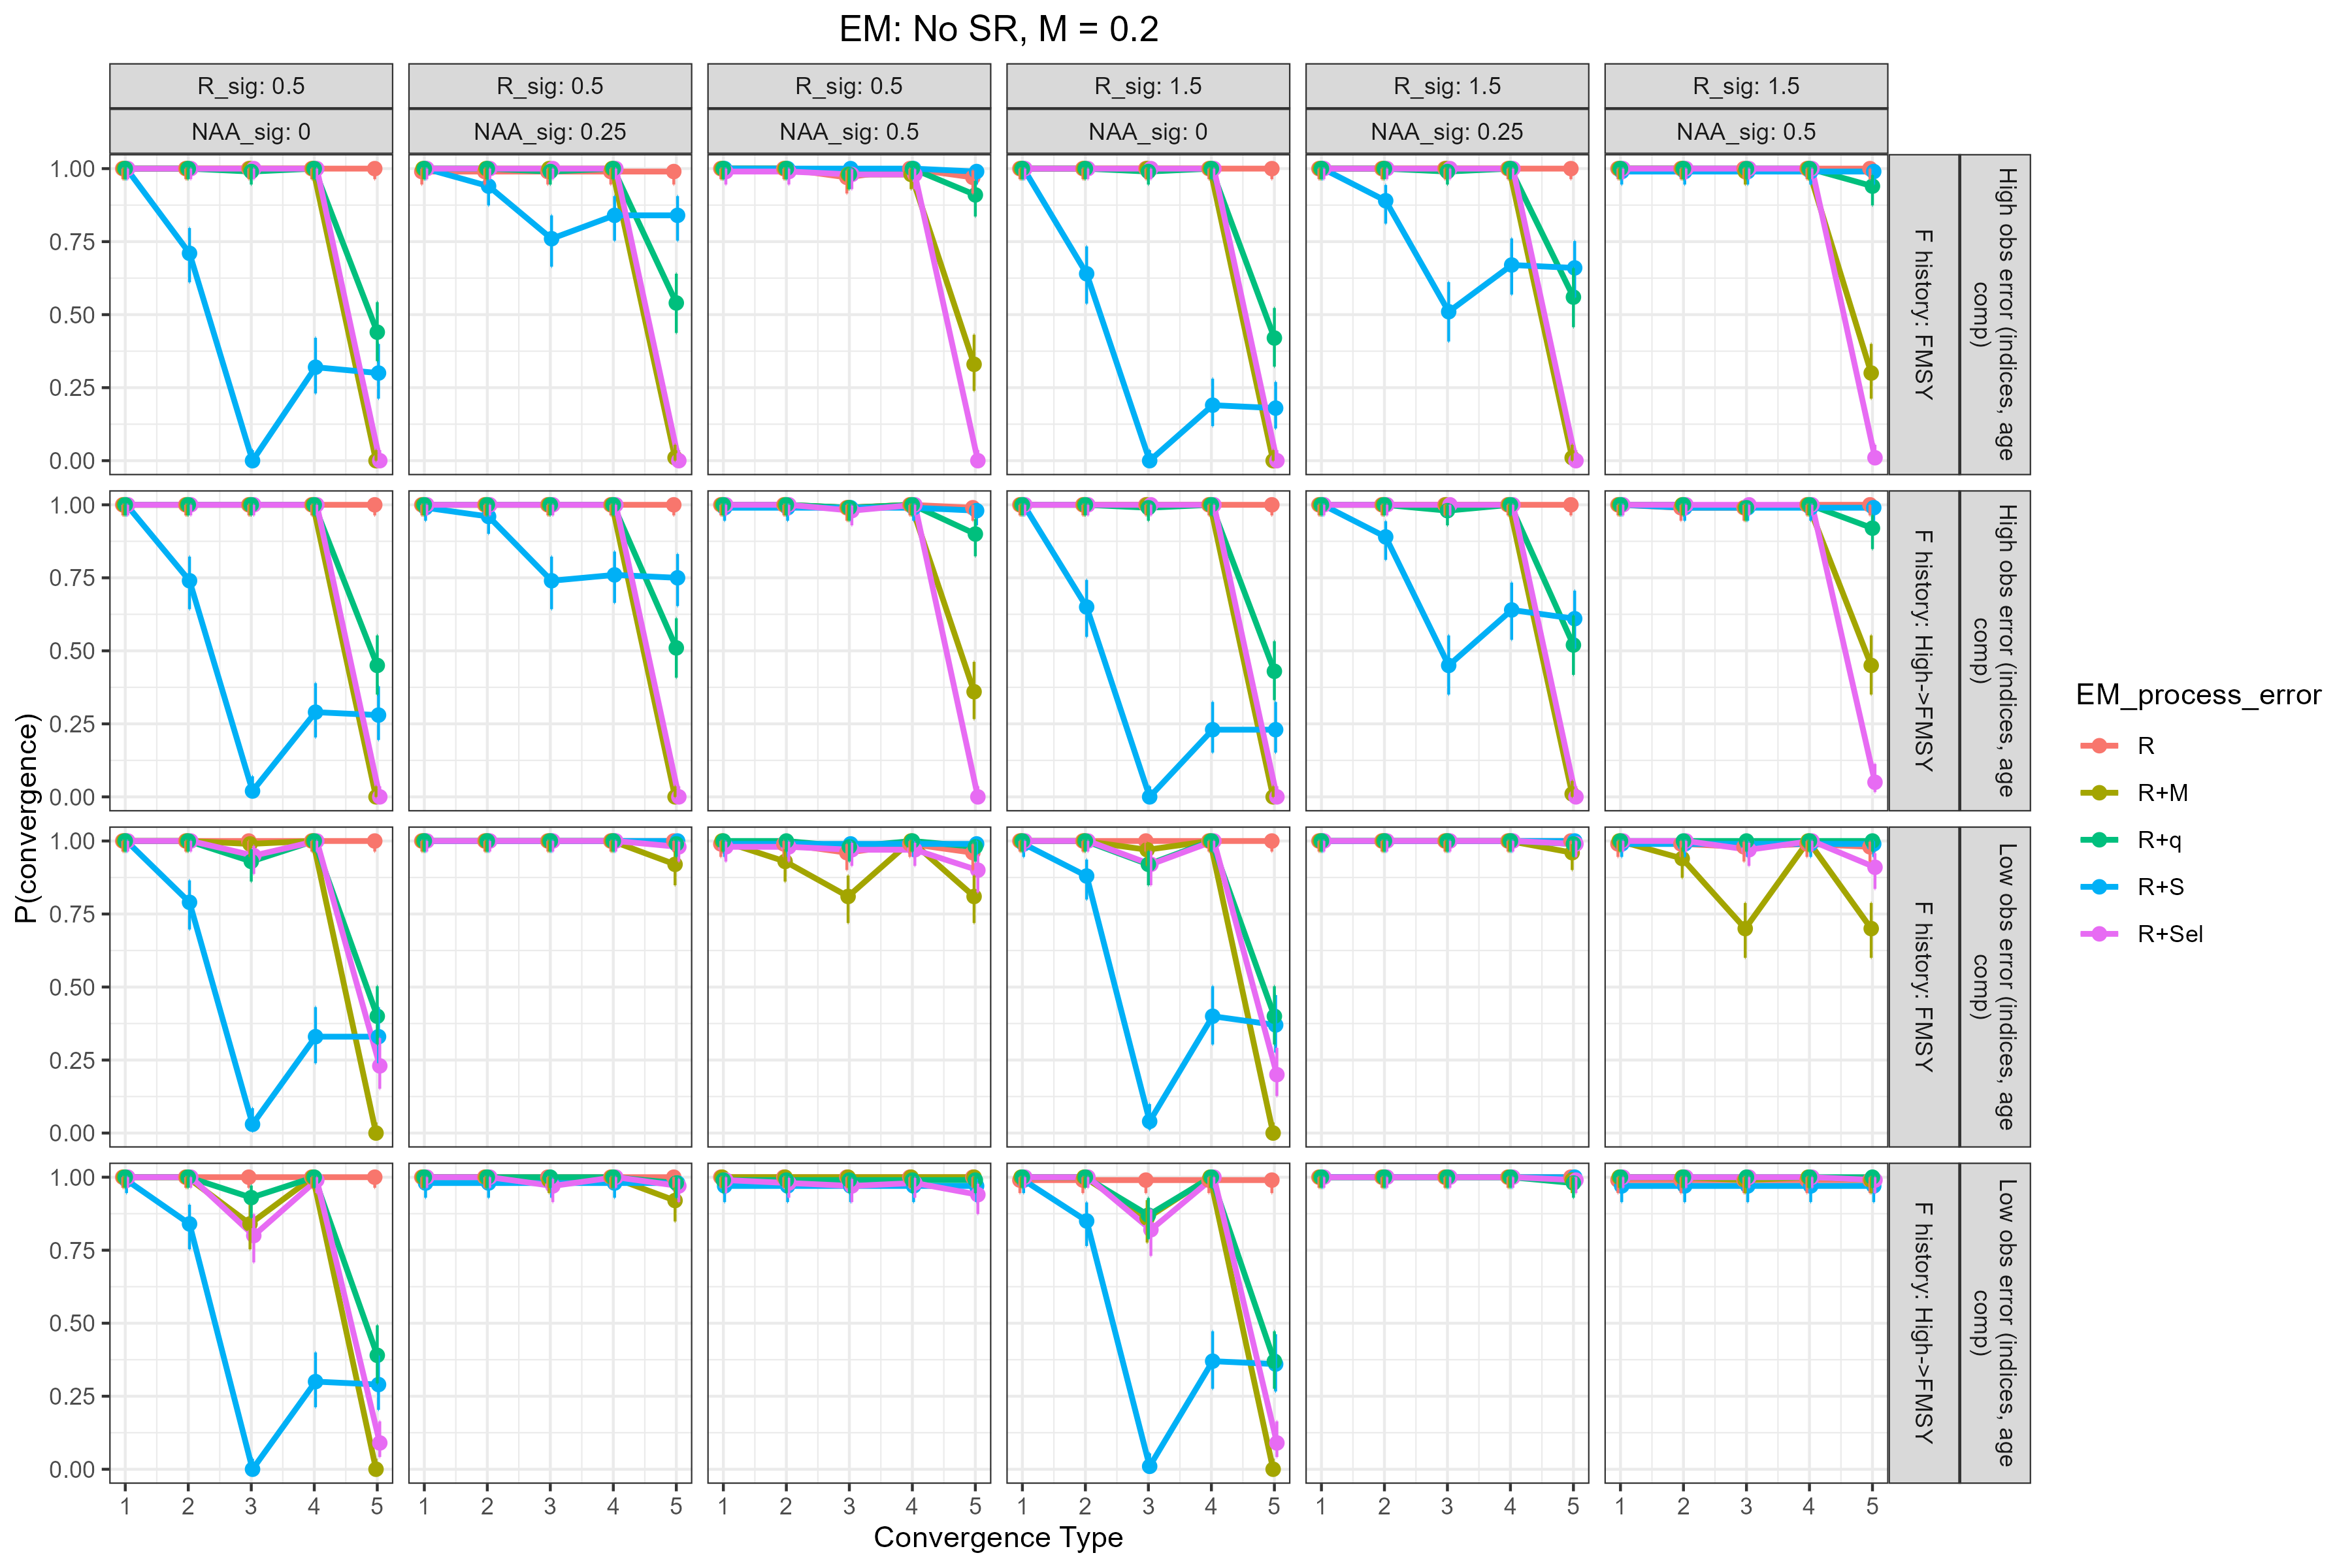
\includegraphics[width = \textwidth]{naa_om_p_convergence_meanR_M_fixed.png}
\end{center}
\end{figure}
\end{landscape}

\begin{landscape}
\begin{figure}
\caption{Probability of each type of convergence of estimating models with alternative process error assumptions for operating models that have process error structures R and R+S. vertical lines represent 95\% confidence intervals. All estimating models estimate mean recruitment rather than a stock-recruit relationship and and M is estimated.}\label{naa_om_em_R_ME_convergence}
\begin{center}
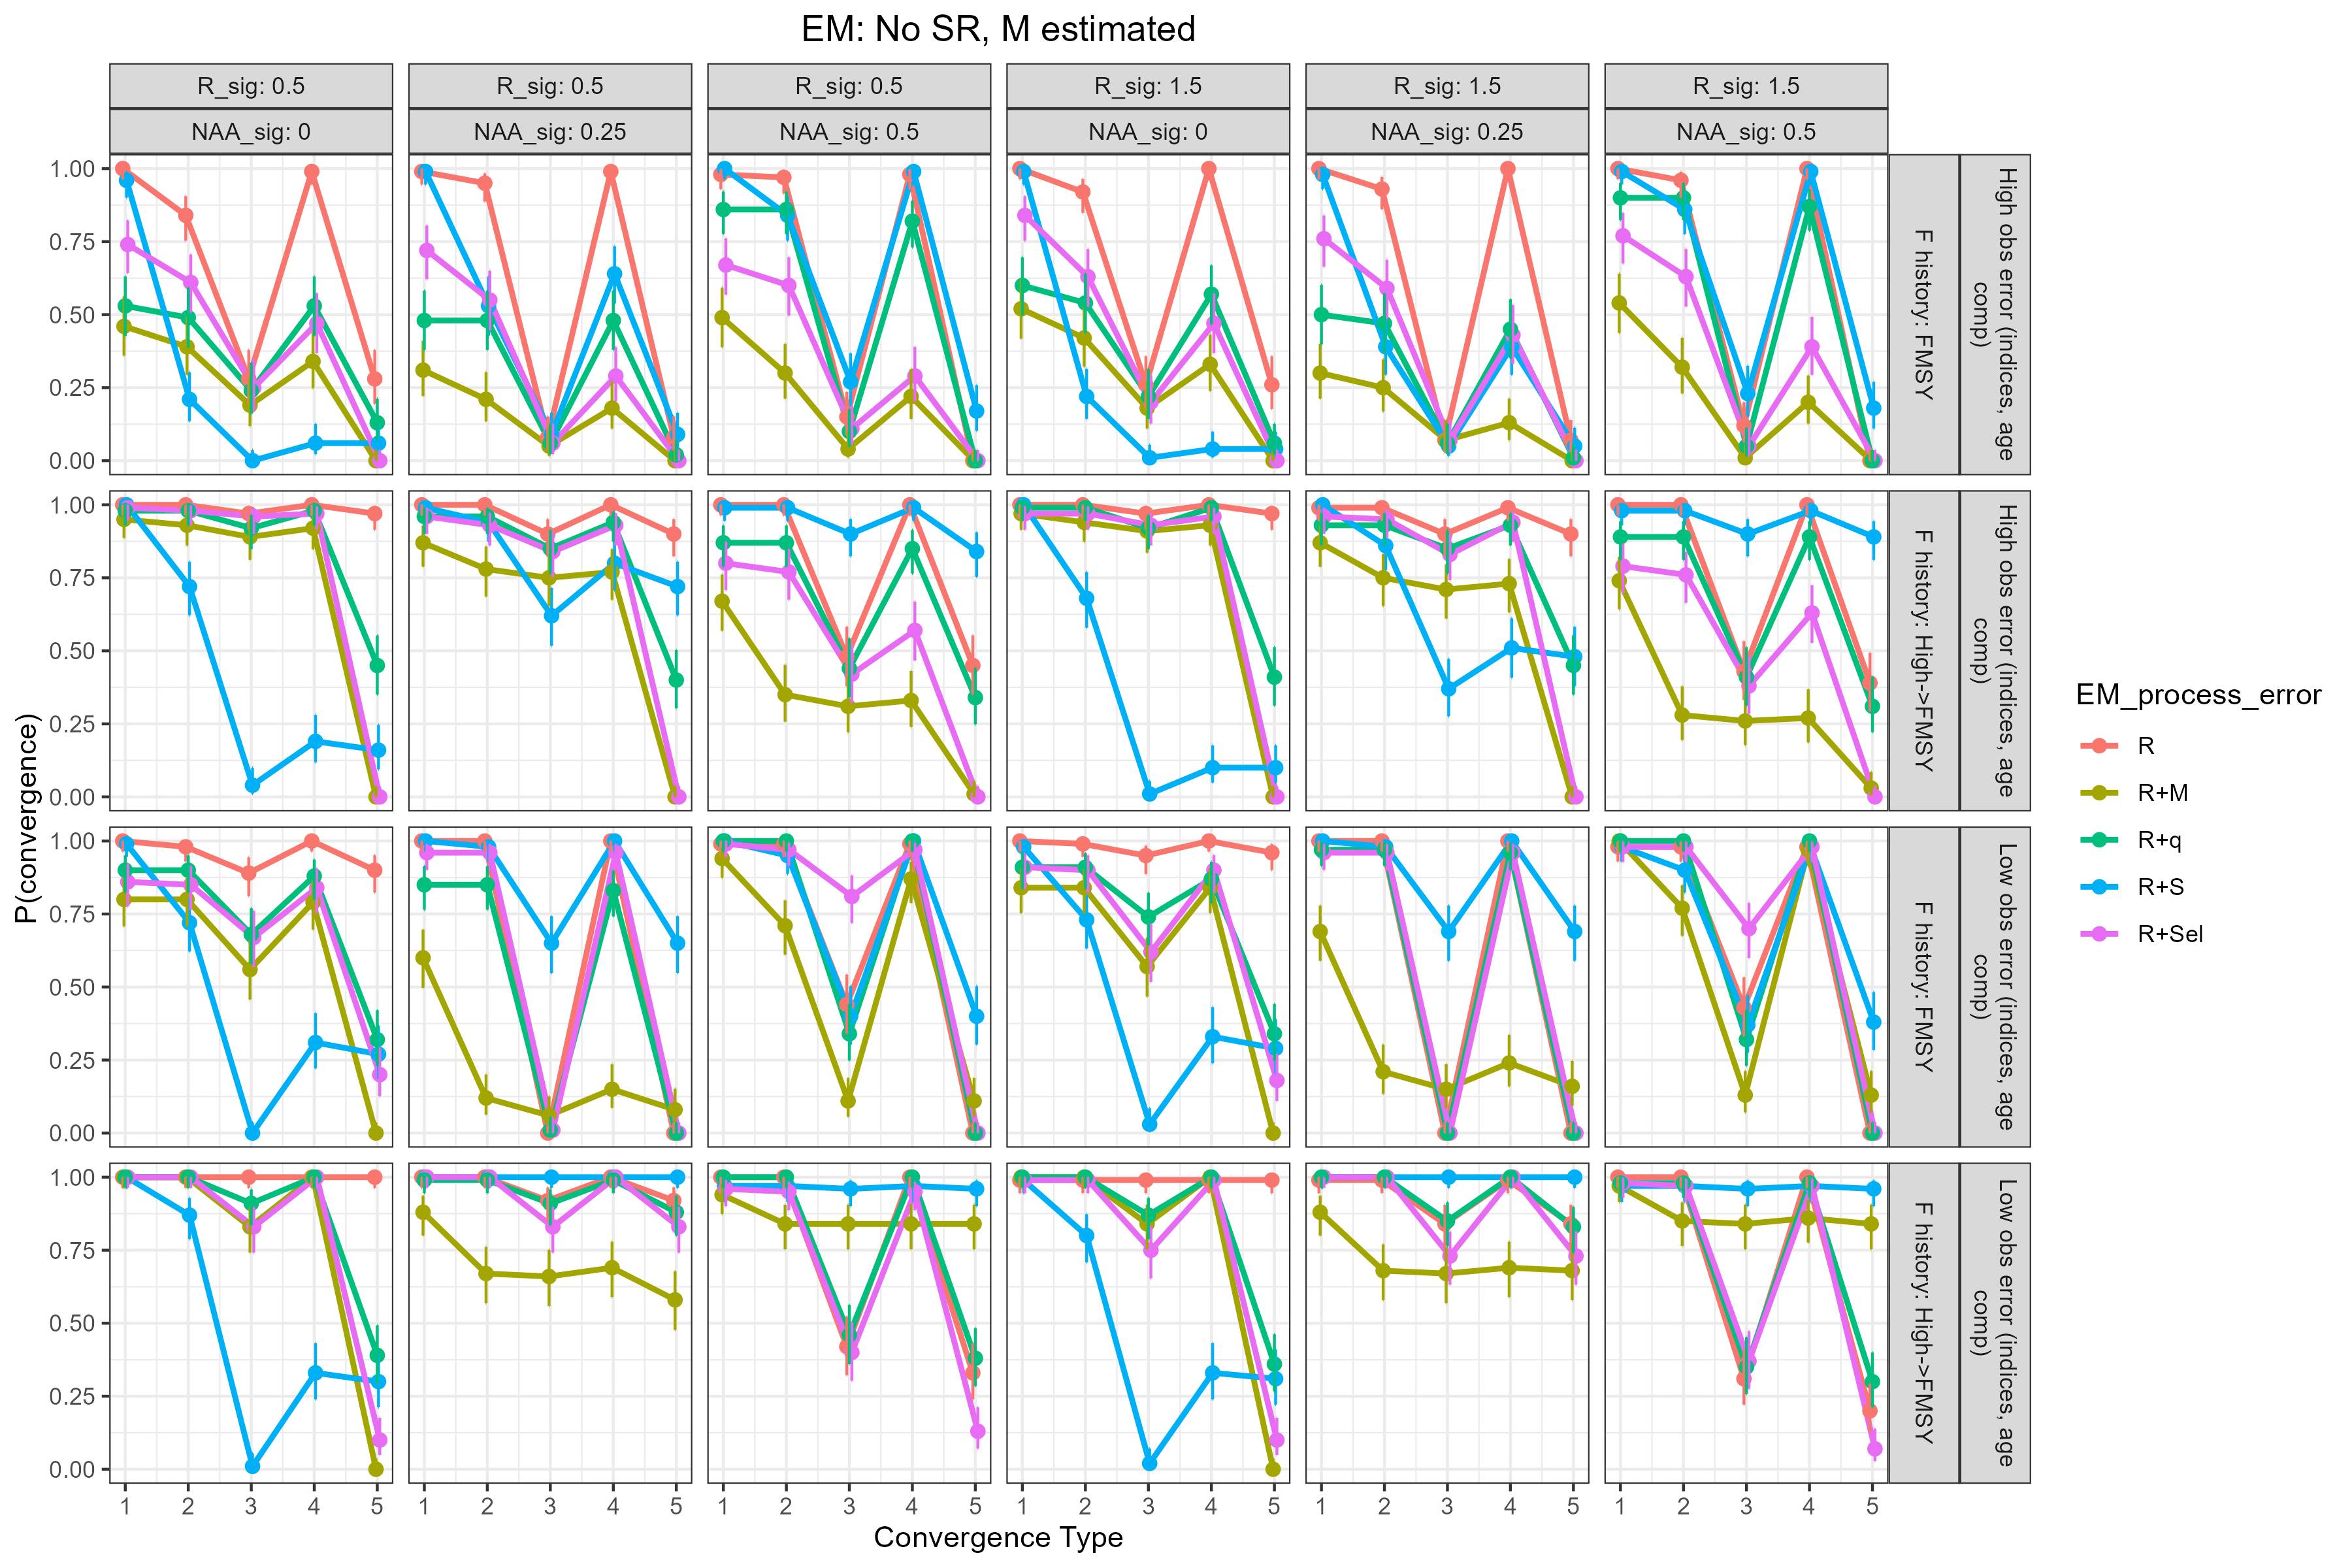
\includegraphics[width = \textwidth]{naa_om_p_convergence_meanR_M_estimated.png}
\end{center}
\end{figure}
\end{landscape}

\begin{landscape}
\begin{figure}
\caption{Probability of each type of convergence of estimating models with alternative process error assumptions for operating models that have process error structures R and R+S. vertical lines represent 95\% confidence intervals. All estimating models estimate a Beverton-Holt stock-recruit relationship and and M is fixed at the true value.}\label{naa_om_em_BH_MF_convergence}
\begin{center}
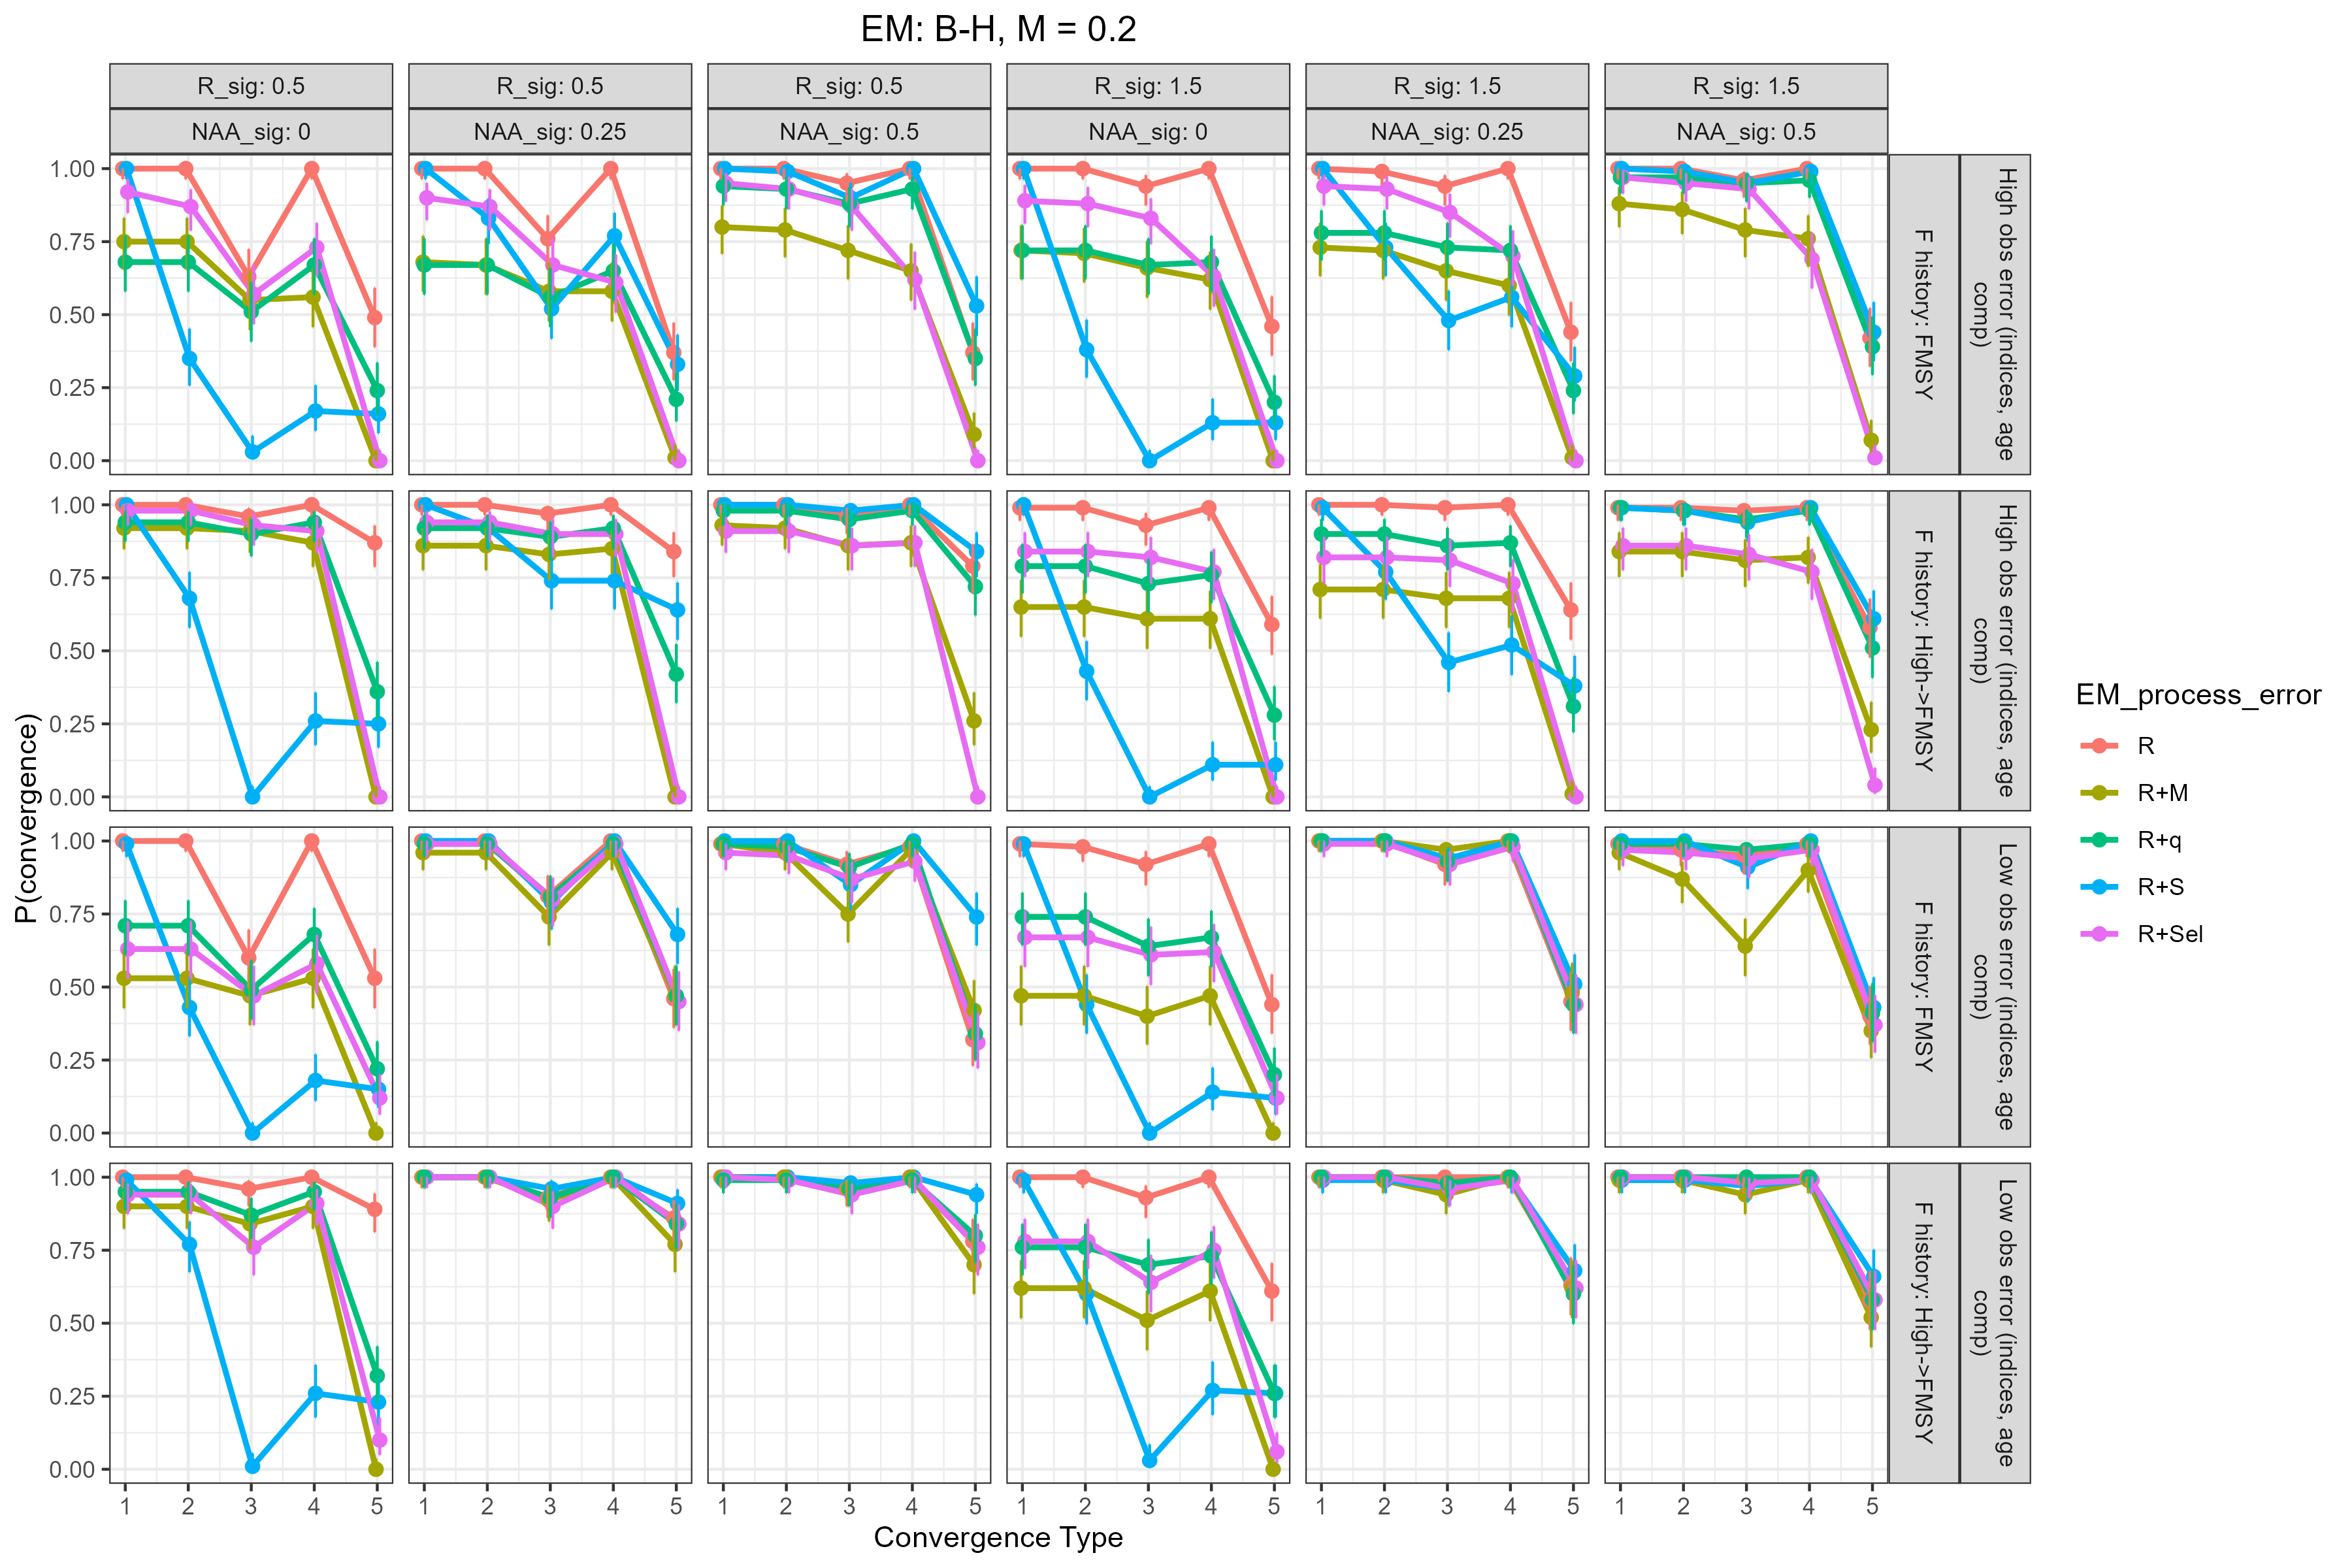
\includegraphics[width = \textwidth]{naa_om_p_convergence_BH_M_fixed.png}
\end{center}
\end{figure}
\end{landscape}

\begin{landscape}
\begin{figure}
\caption{Probability of each type of convergence of estimating models with alternative process error assumptions for operating models that have process error structures R and R+S. vertical lines represent 95\% confidence intervals. All estimating models estimate a Beverton-Holt stock-recruit relationship and and M is estimated.}\label{naa_om_em_BH_ME_convergence}
\begin{center}
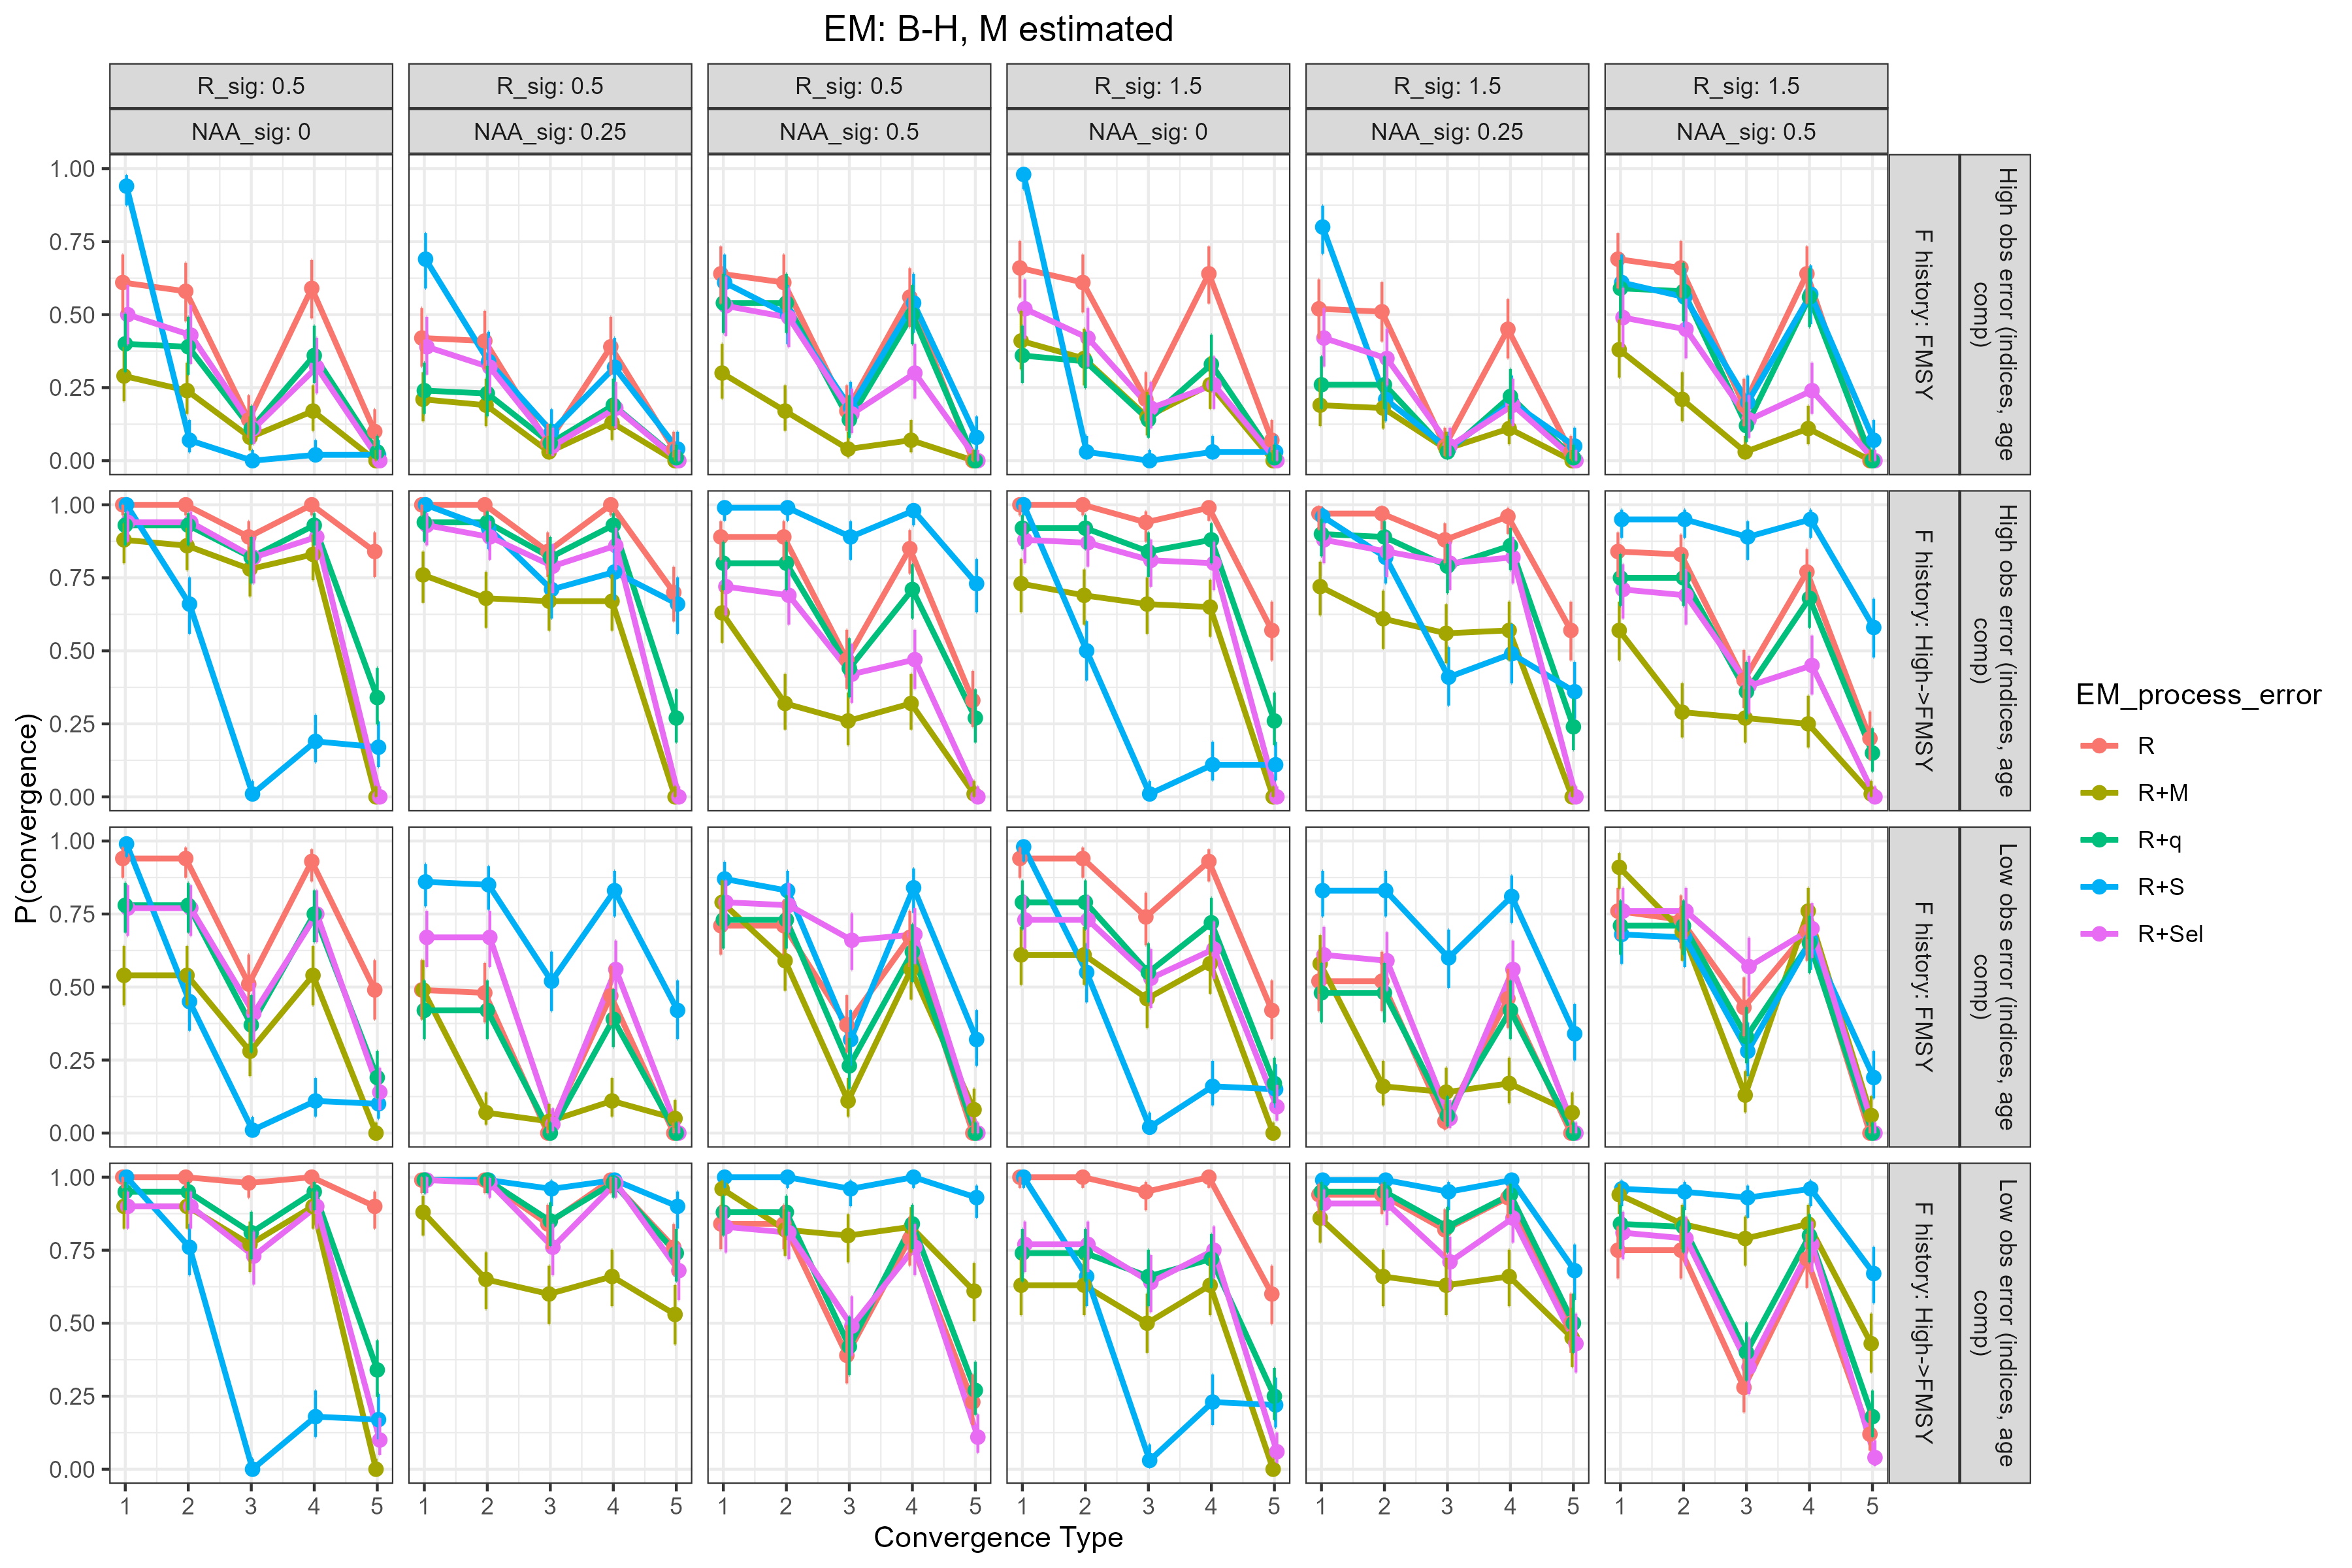
\includegraphics[width = \textwidth]{naa_om_p_convergence_BH_M_estimated.png}
\end{center}
\end{figure}
\end{landscape}

\hypertarget{rm-operating-models}{%
\subsubsection*{R+M operating models}\label{rm-operating-models}}
\addcontentsline{toc}{subsubsection}{R+M operating models}

Figures \ref{M_om_em_R_MF_convergence} to
\ref{M_om_em_BH_ME_convergence}

\begin{landscape}
\begin{figure}
\caption{Probability of each type of convergence of estimating models with alternative process error assumptions for operating models that have process error structure R+M. vertical lines represent 95\% confidence intervals. All estimating models estimate mean recruitment rather than a stock-recruit relationship and and M is fixed at the true value.}\label{M_om_em_R_MF_convergence}
\begin{center}
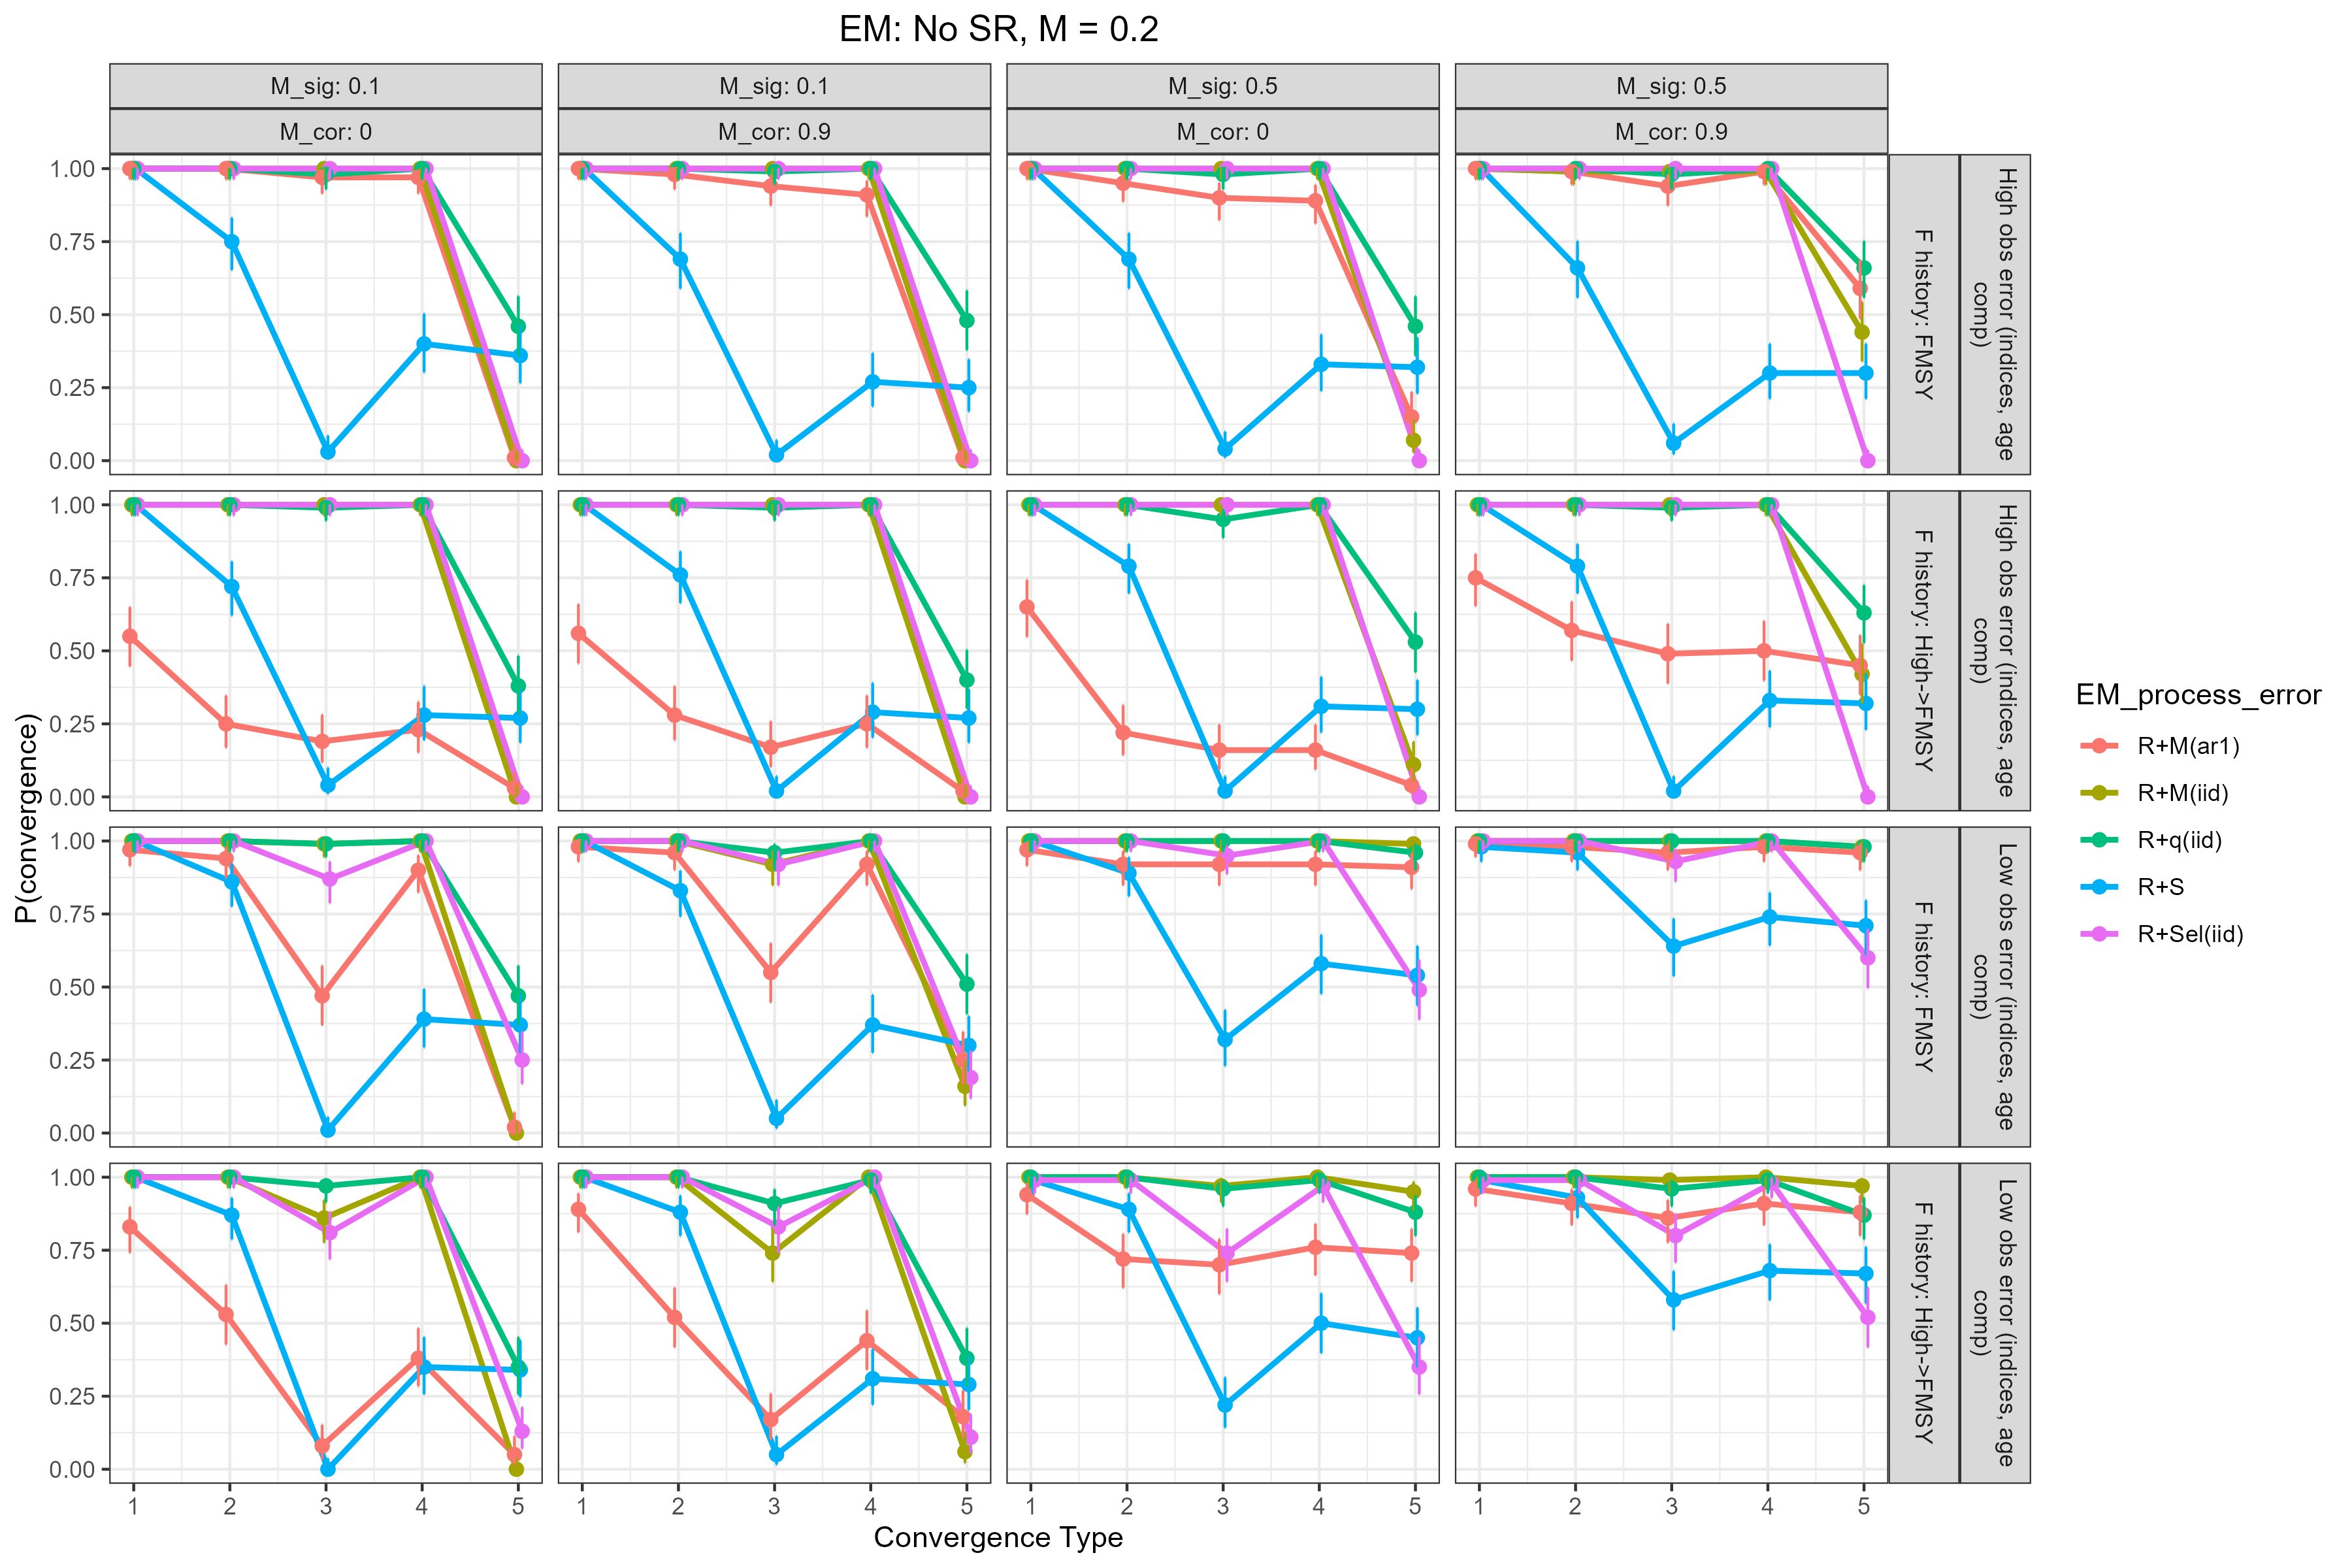
\includegraphics[width = \textwidth]{M_om_p_convergence_meanR_M_fixed.png}
\end{center}
\end{figure}
\end{landscape}

\begin{landscape}
\begin{figure}
\caption{Probability of each type of convergence of estimating models with alternative process error assumptions for operating models that have process error structure R+M. vertical lines represent 95\% confidence intervals. All estimating models estimate mean recruitment rather than a stock-recruit relationship and and M is estimated.}\label{M_om_em_R_ME_convergence}
\begin{center}
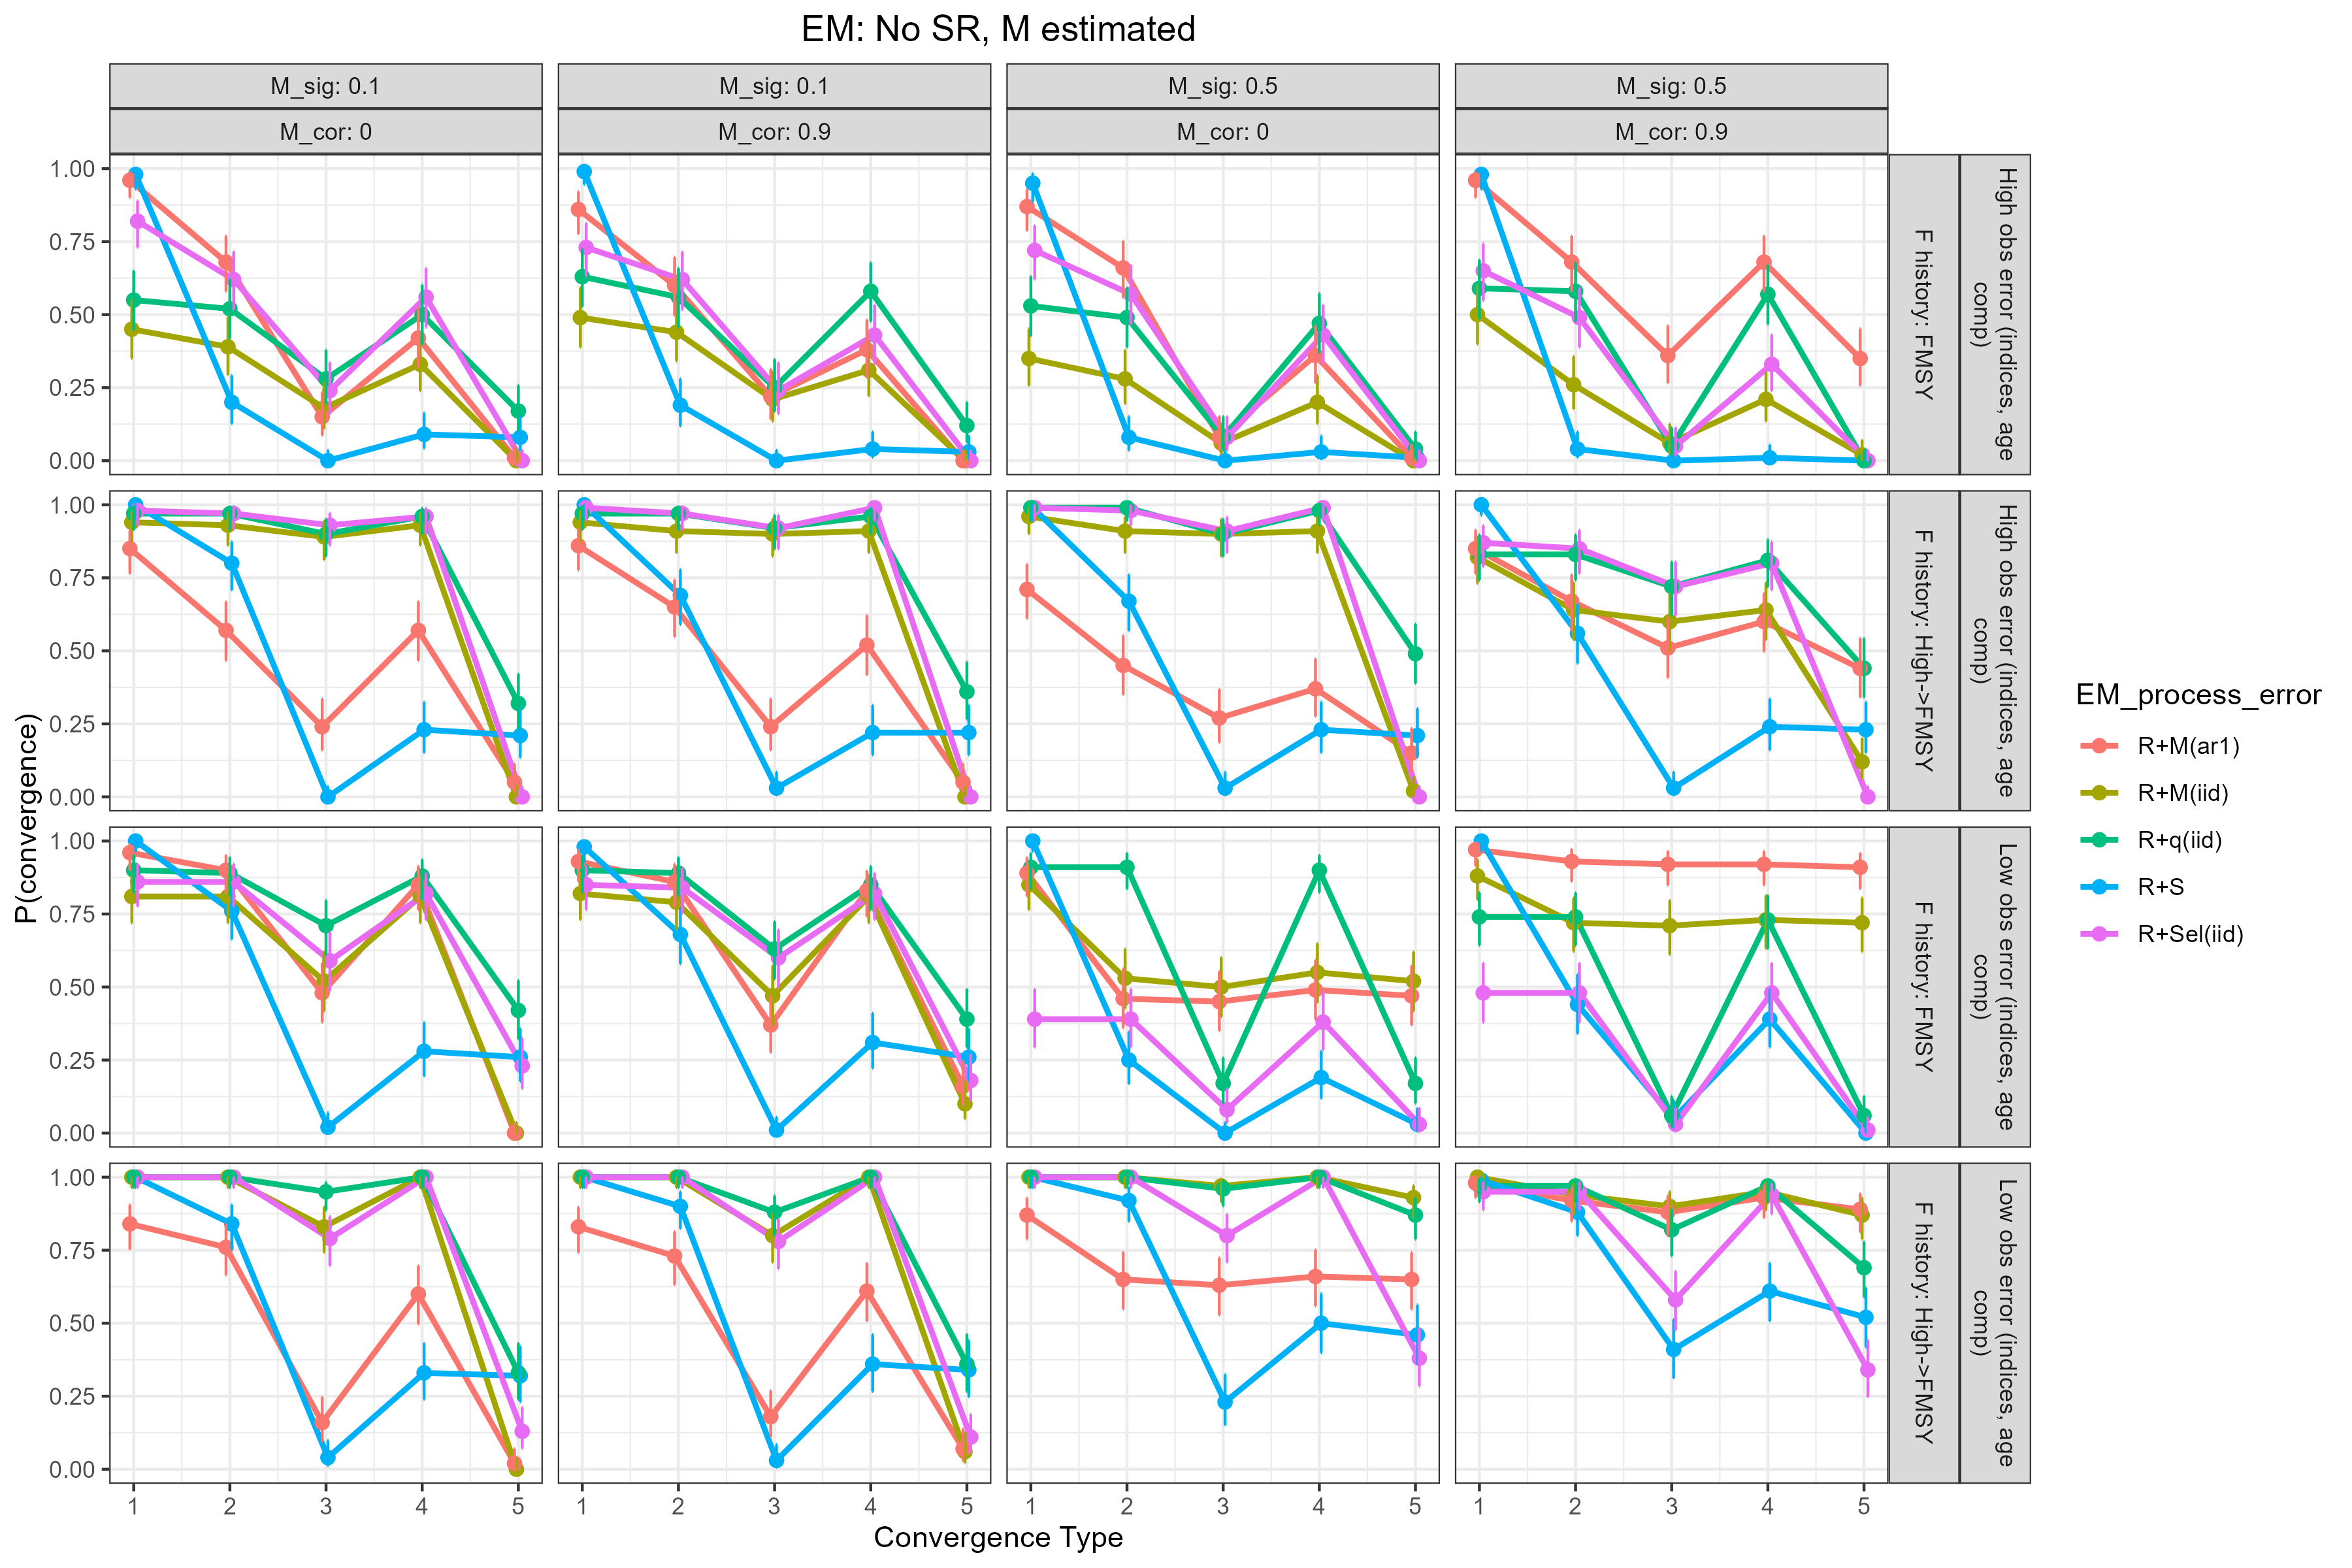
\includegraphics[width = \textwidth]{M_om_p_convergence_meanR_M_estimated.png}
\end{center}
\end{figure}
\end{landscape}

\begin{landscape}
\begin{figure}
\caption{Probability of each type of convergence of estimating models with alternative process error assumptions for operating models that have process error structure R+M. vertical lines represent 95\% confidence intervals. All estimating models estimate a Beverton-Holt stock-recruit relationship and and M is fixed at the true value.}\label{M_om_em_BH_MF_convergence}
\begin{center}
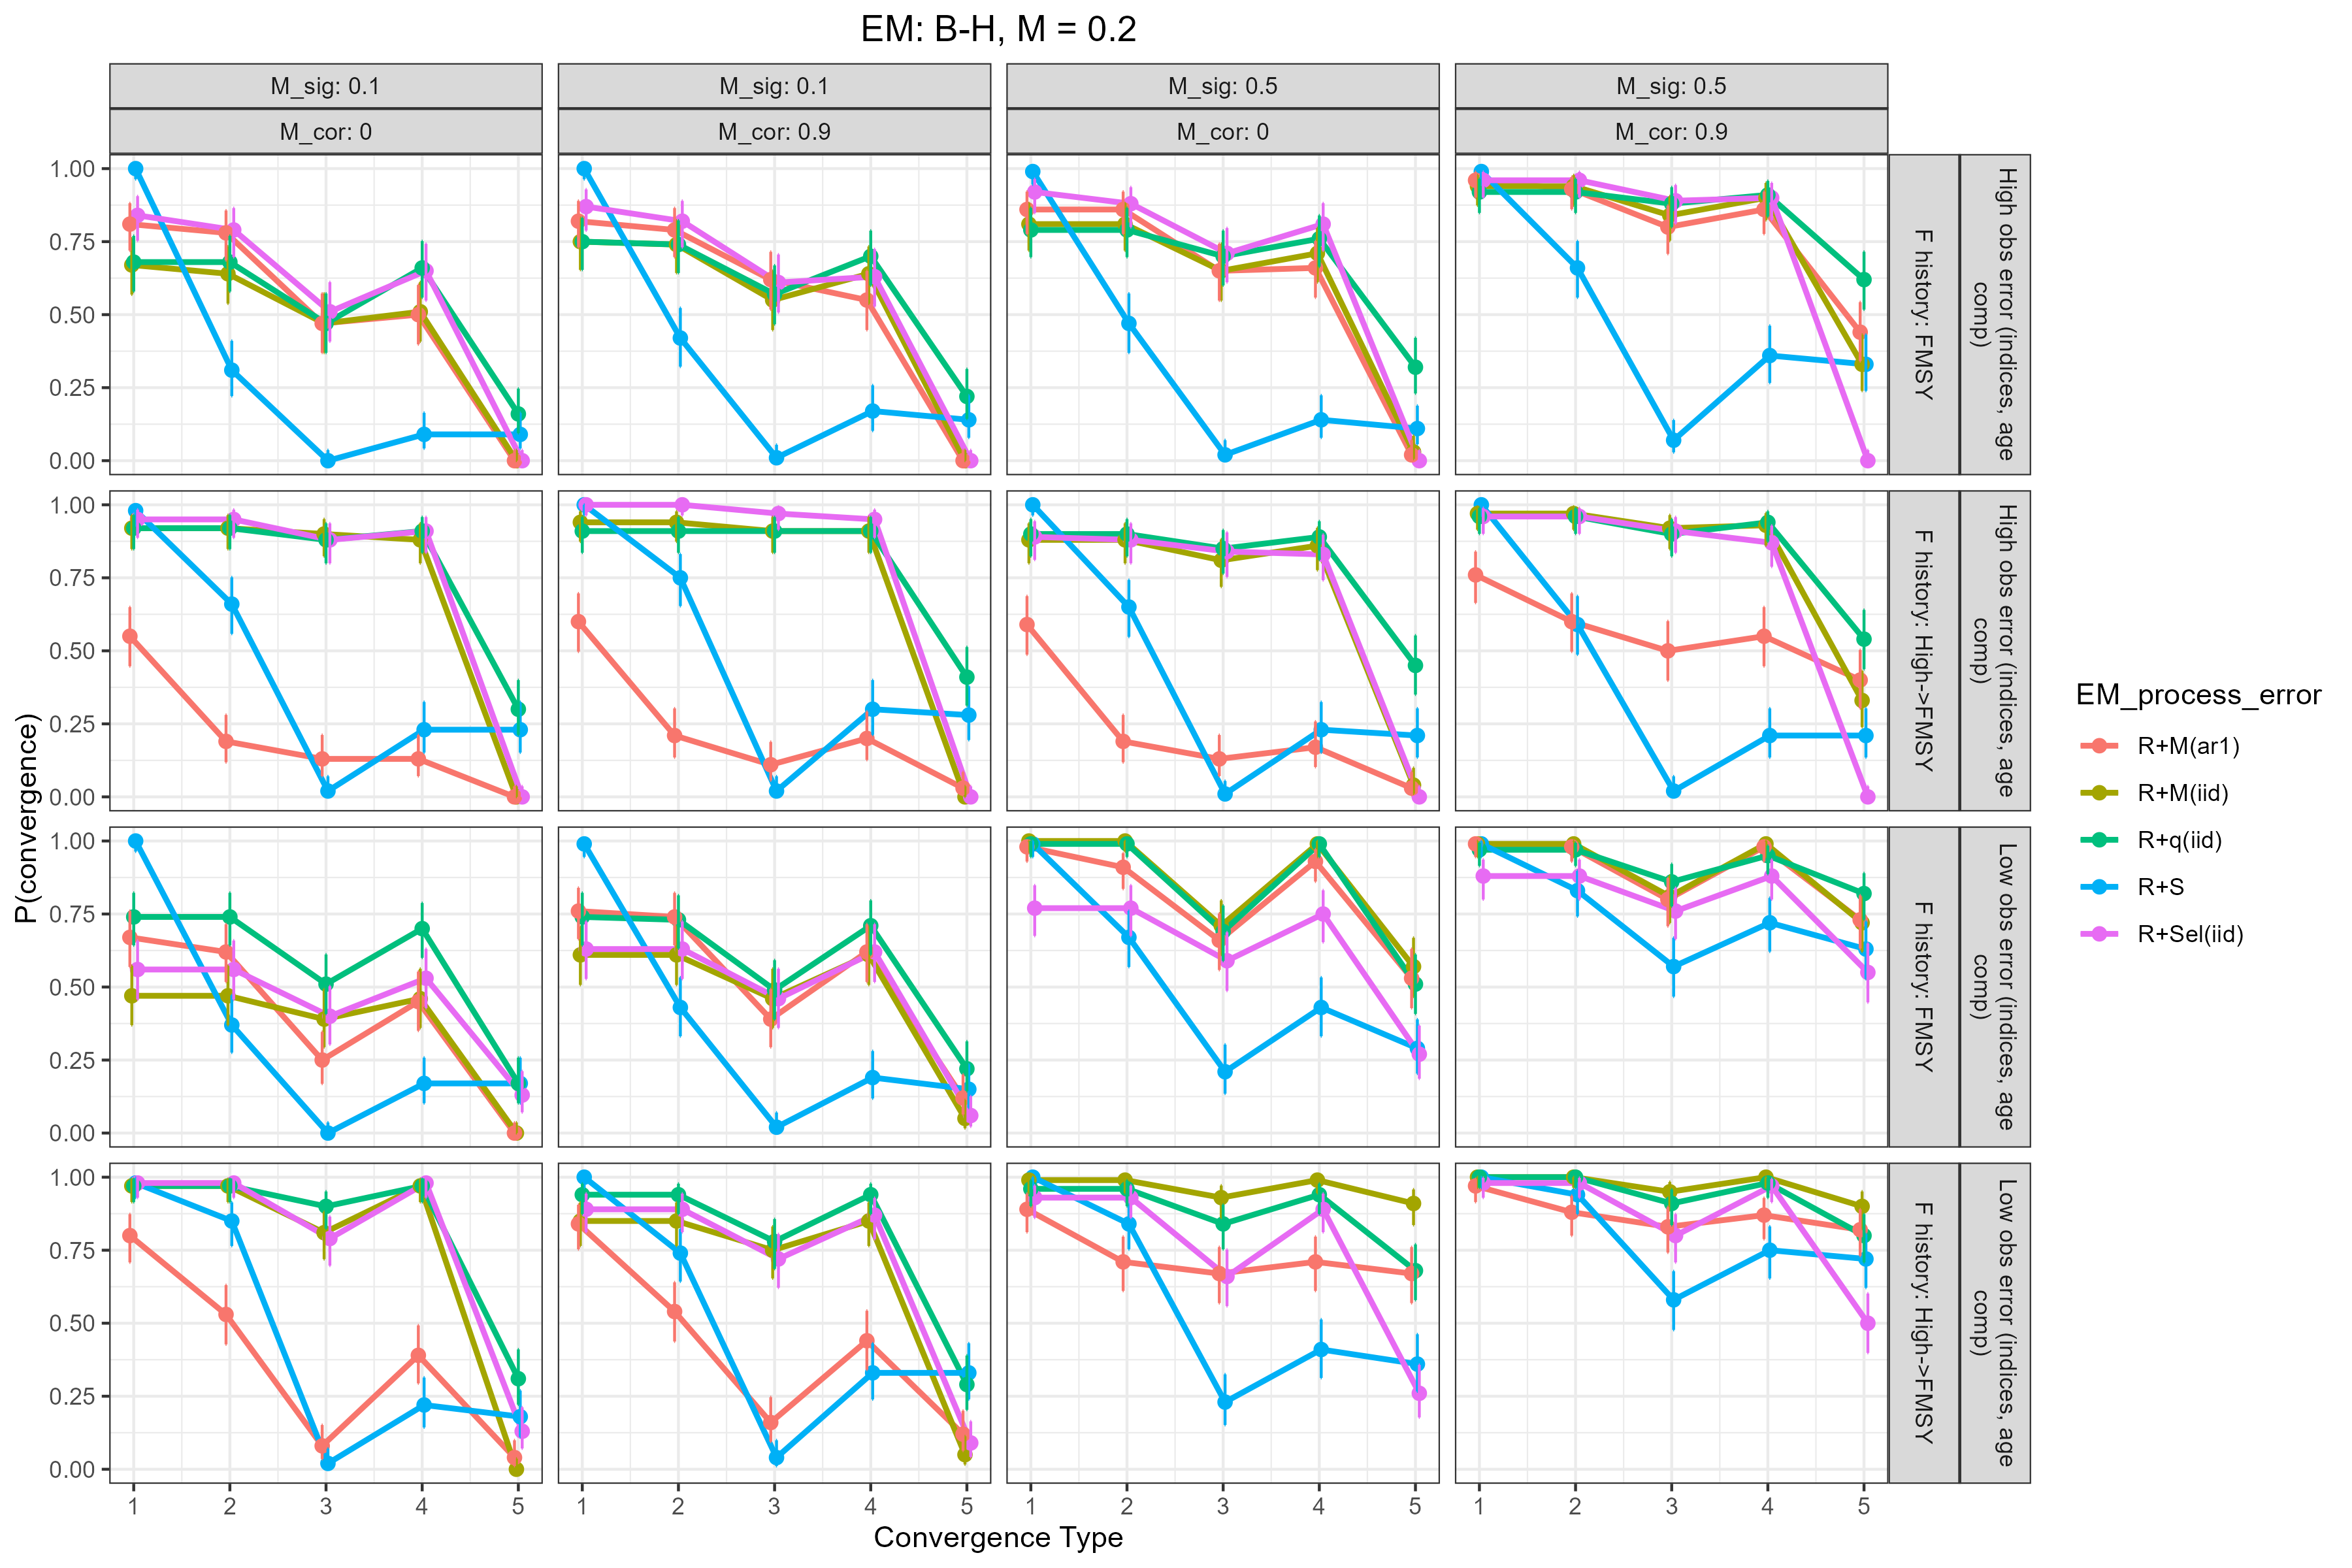
\includegraphics[width = \textwidth]{M_om_p_convergence_BH_M_fixed.png}
\end{center}
\end{figure}
\end{landscape}

\begin{landscape}
\begin{figure}
\caption{Probability of each type of convergence of estimating models with alternative process error assumptions for operating models that have process error structure R+M. vertical lines represent 95\% confidence intervals. All estimating models estimate a Beverton-Holt stock-recruit relationship and and M is estimated.}\label{M_om_em_BH_ME_convergence}
\begin{center}
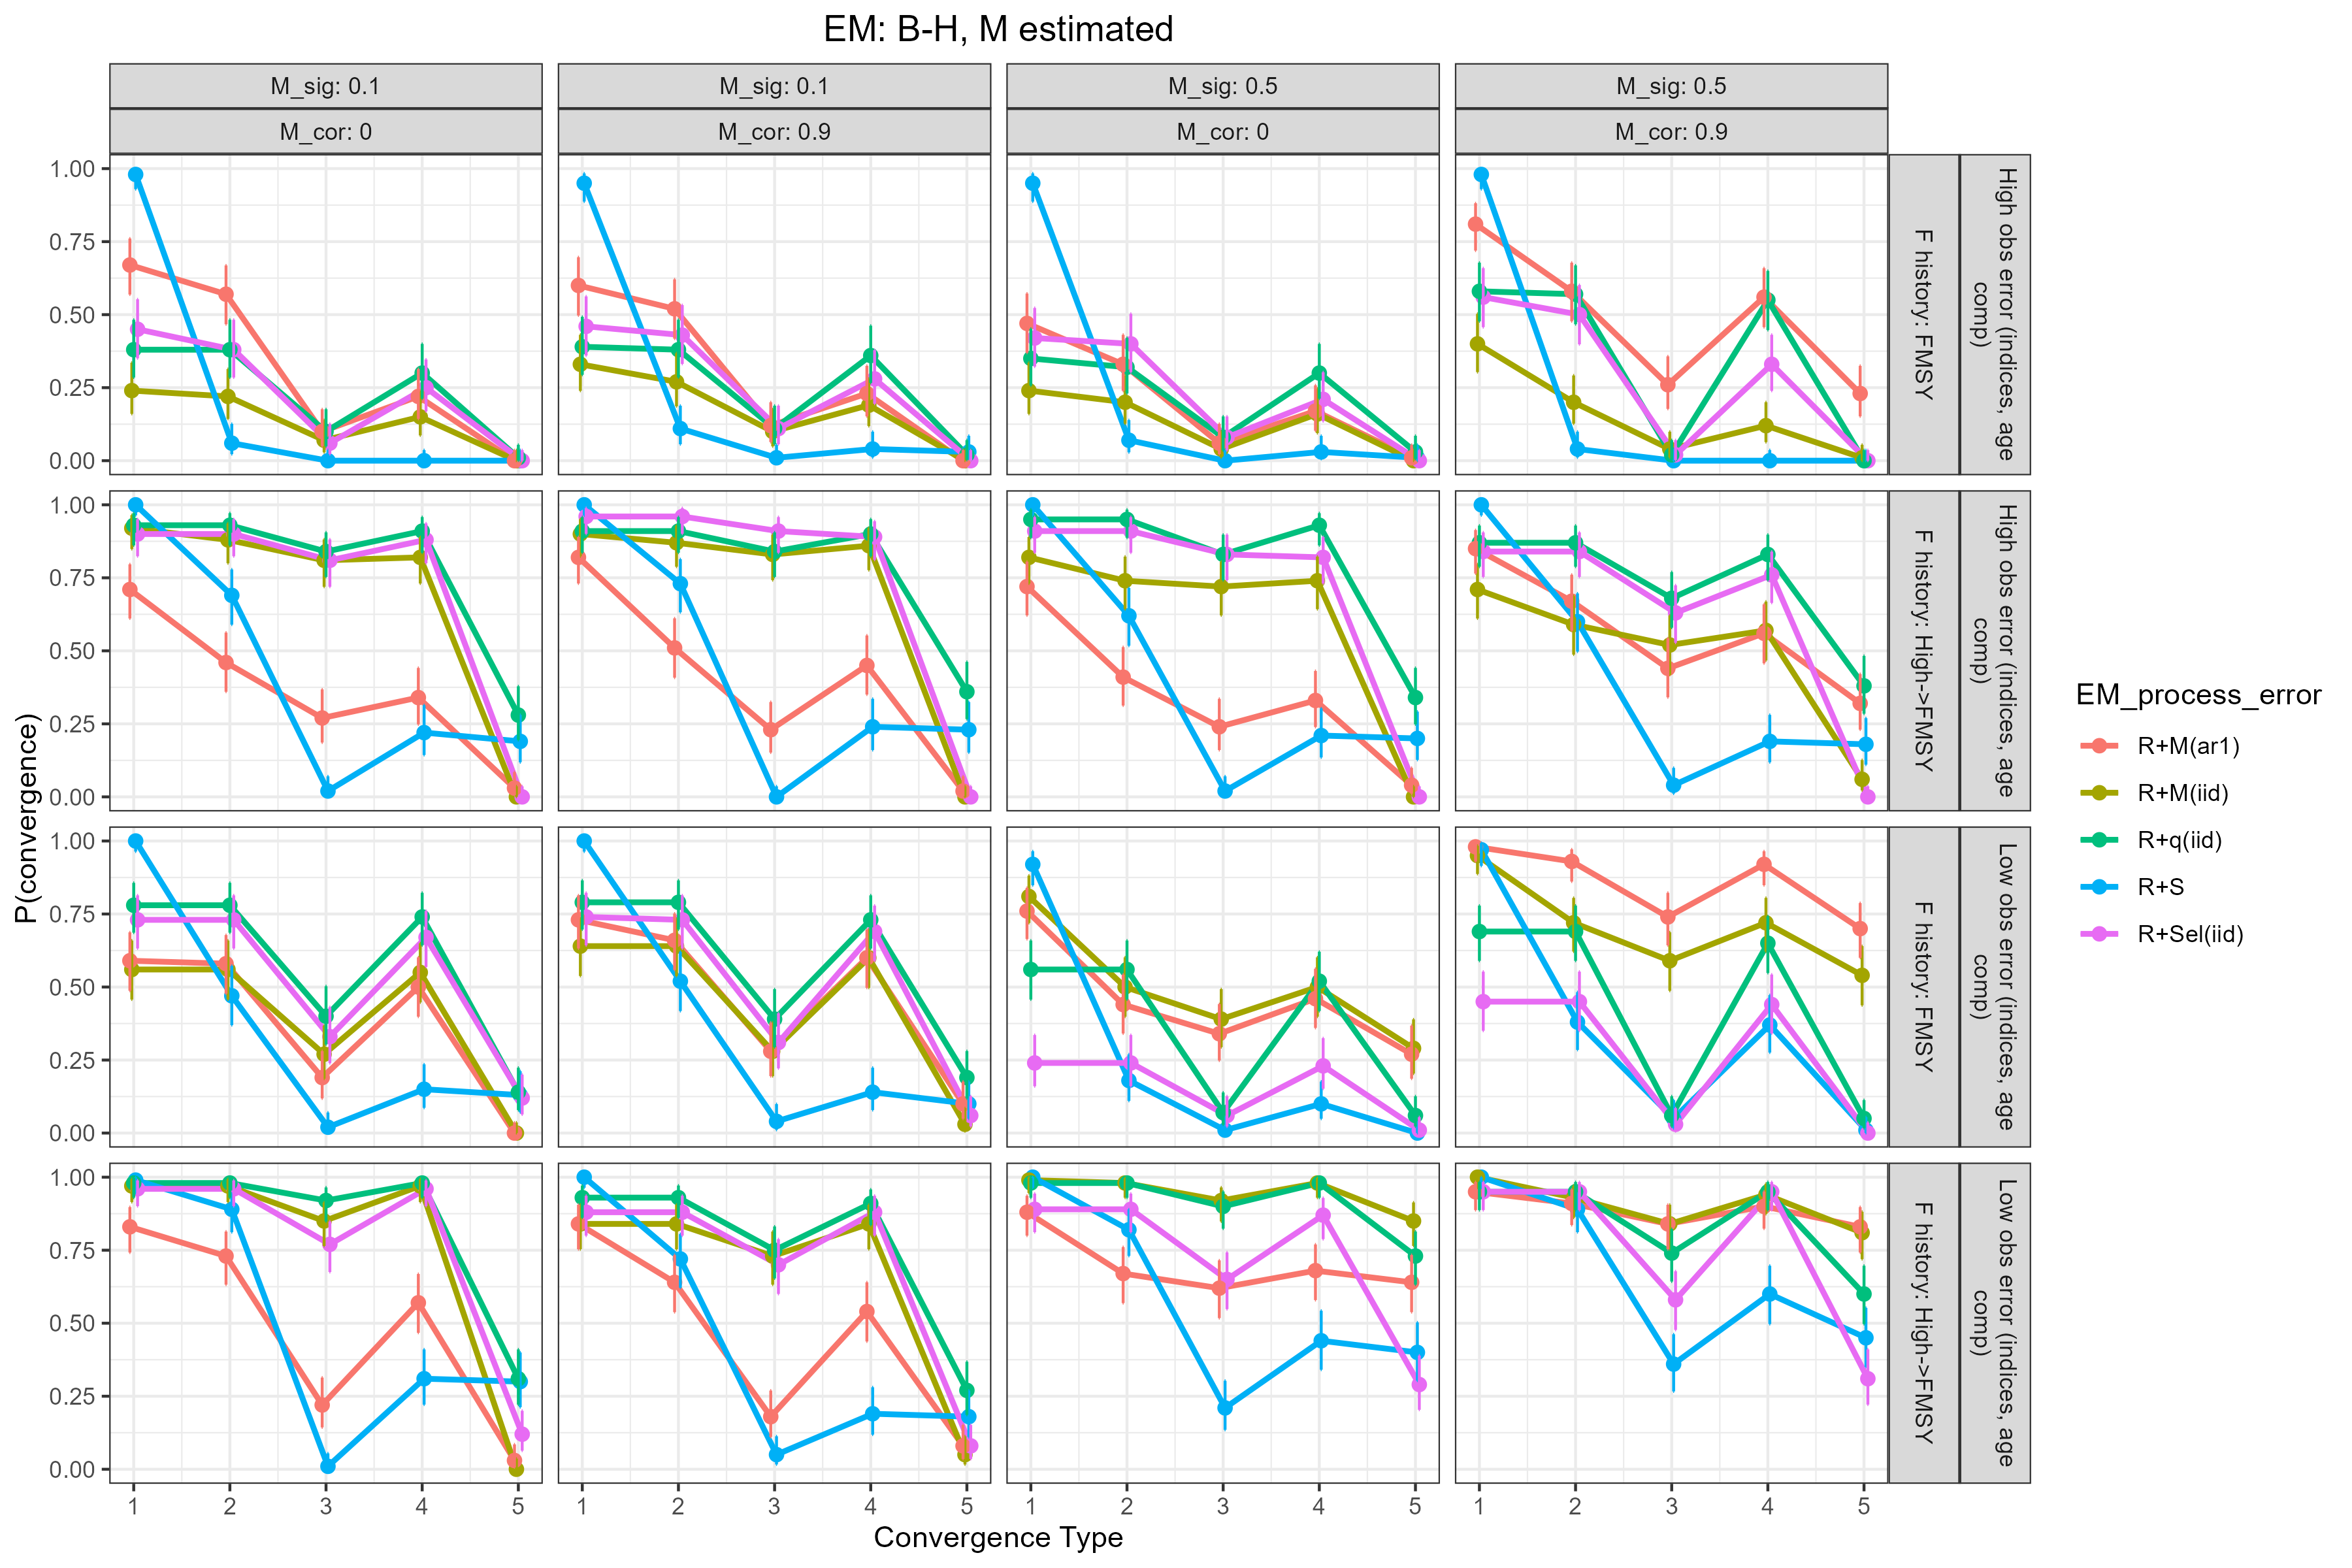
\includegraphics[width = \textwidth]{M_om_p_convergence_BH_M_estimated.png}
\end{center}
\end{figure}
\end{landscape}

\hypertarget{rsel-operating-models}{%
\subsubsection*{R+Sel operating models}\label{rsel-operating-models}}
\addcontentsline{toc}{subsubsection}{R+Sel operating models}

Figures \ref{Sel_om_em_R_MF_convergence} to
\ref{Sel_om_em_BH_ME_convergence}

\begin{landscape}
\begin{figure}
\caption{Probability of each type of convergence of estimating models with alternative process error assumptions for operating models that have process error structure R+Sel. vertical lines represent 95\% confidence intervals. All estimating models estimate mean recruitment rather than a stock-recruit relationship and and M is fixed at the true value.}\label{Sel_om_em_R_MF_convergence}
\begin{center}
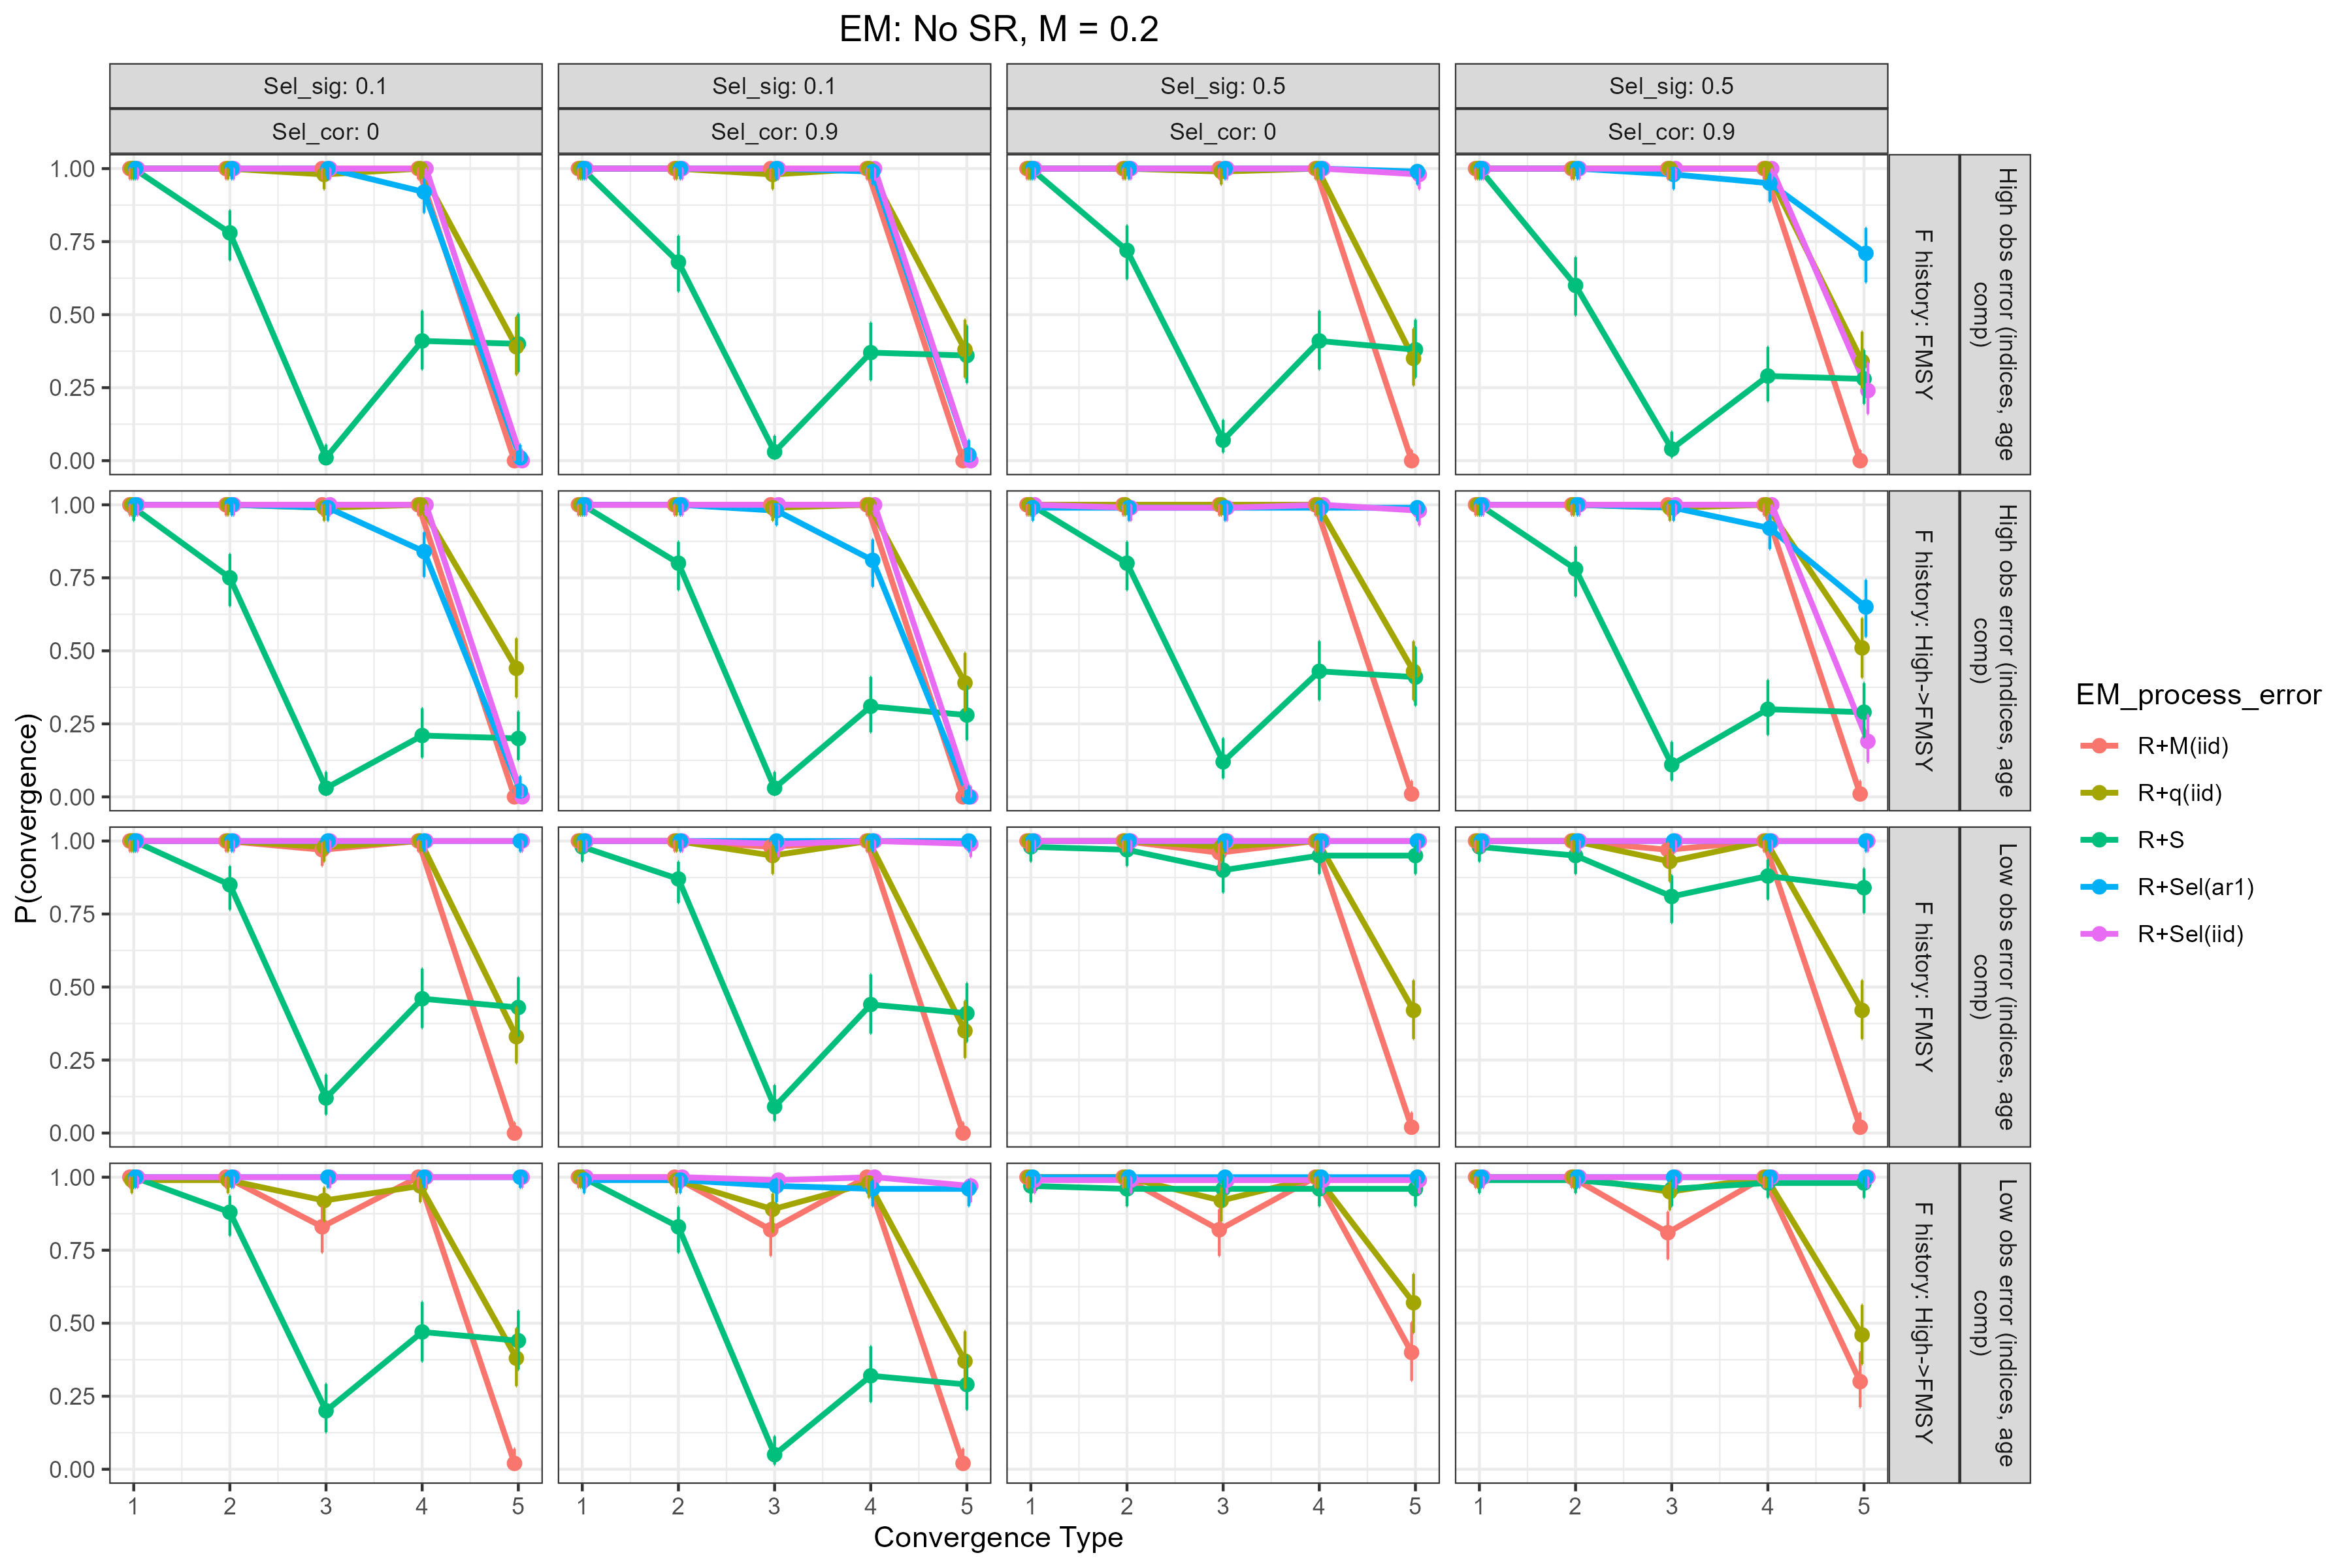
\includegraphics[width = \textwidth]{Sel_om_p_convergence_meanR_M_fixed.png}
\end{center}
\end{figure}
\end{landscape}

\begin{landscape}
\begin{figure}
\caption{Probability of each type of convergence of estimating models with alternative process error assumptions for operating models that have process error structure R+Sel. vertical lines represent 95\% confidence intervals. All estimating models estimate mean recruitment rather than a stock-recruit relationship and and M is estimated.}\label{Sel_om_em_R_ME_convergence}
\begin{center}
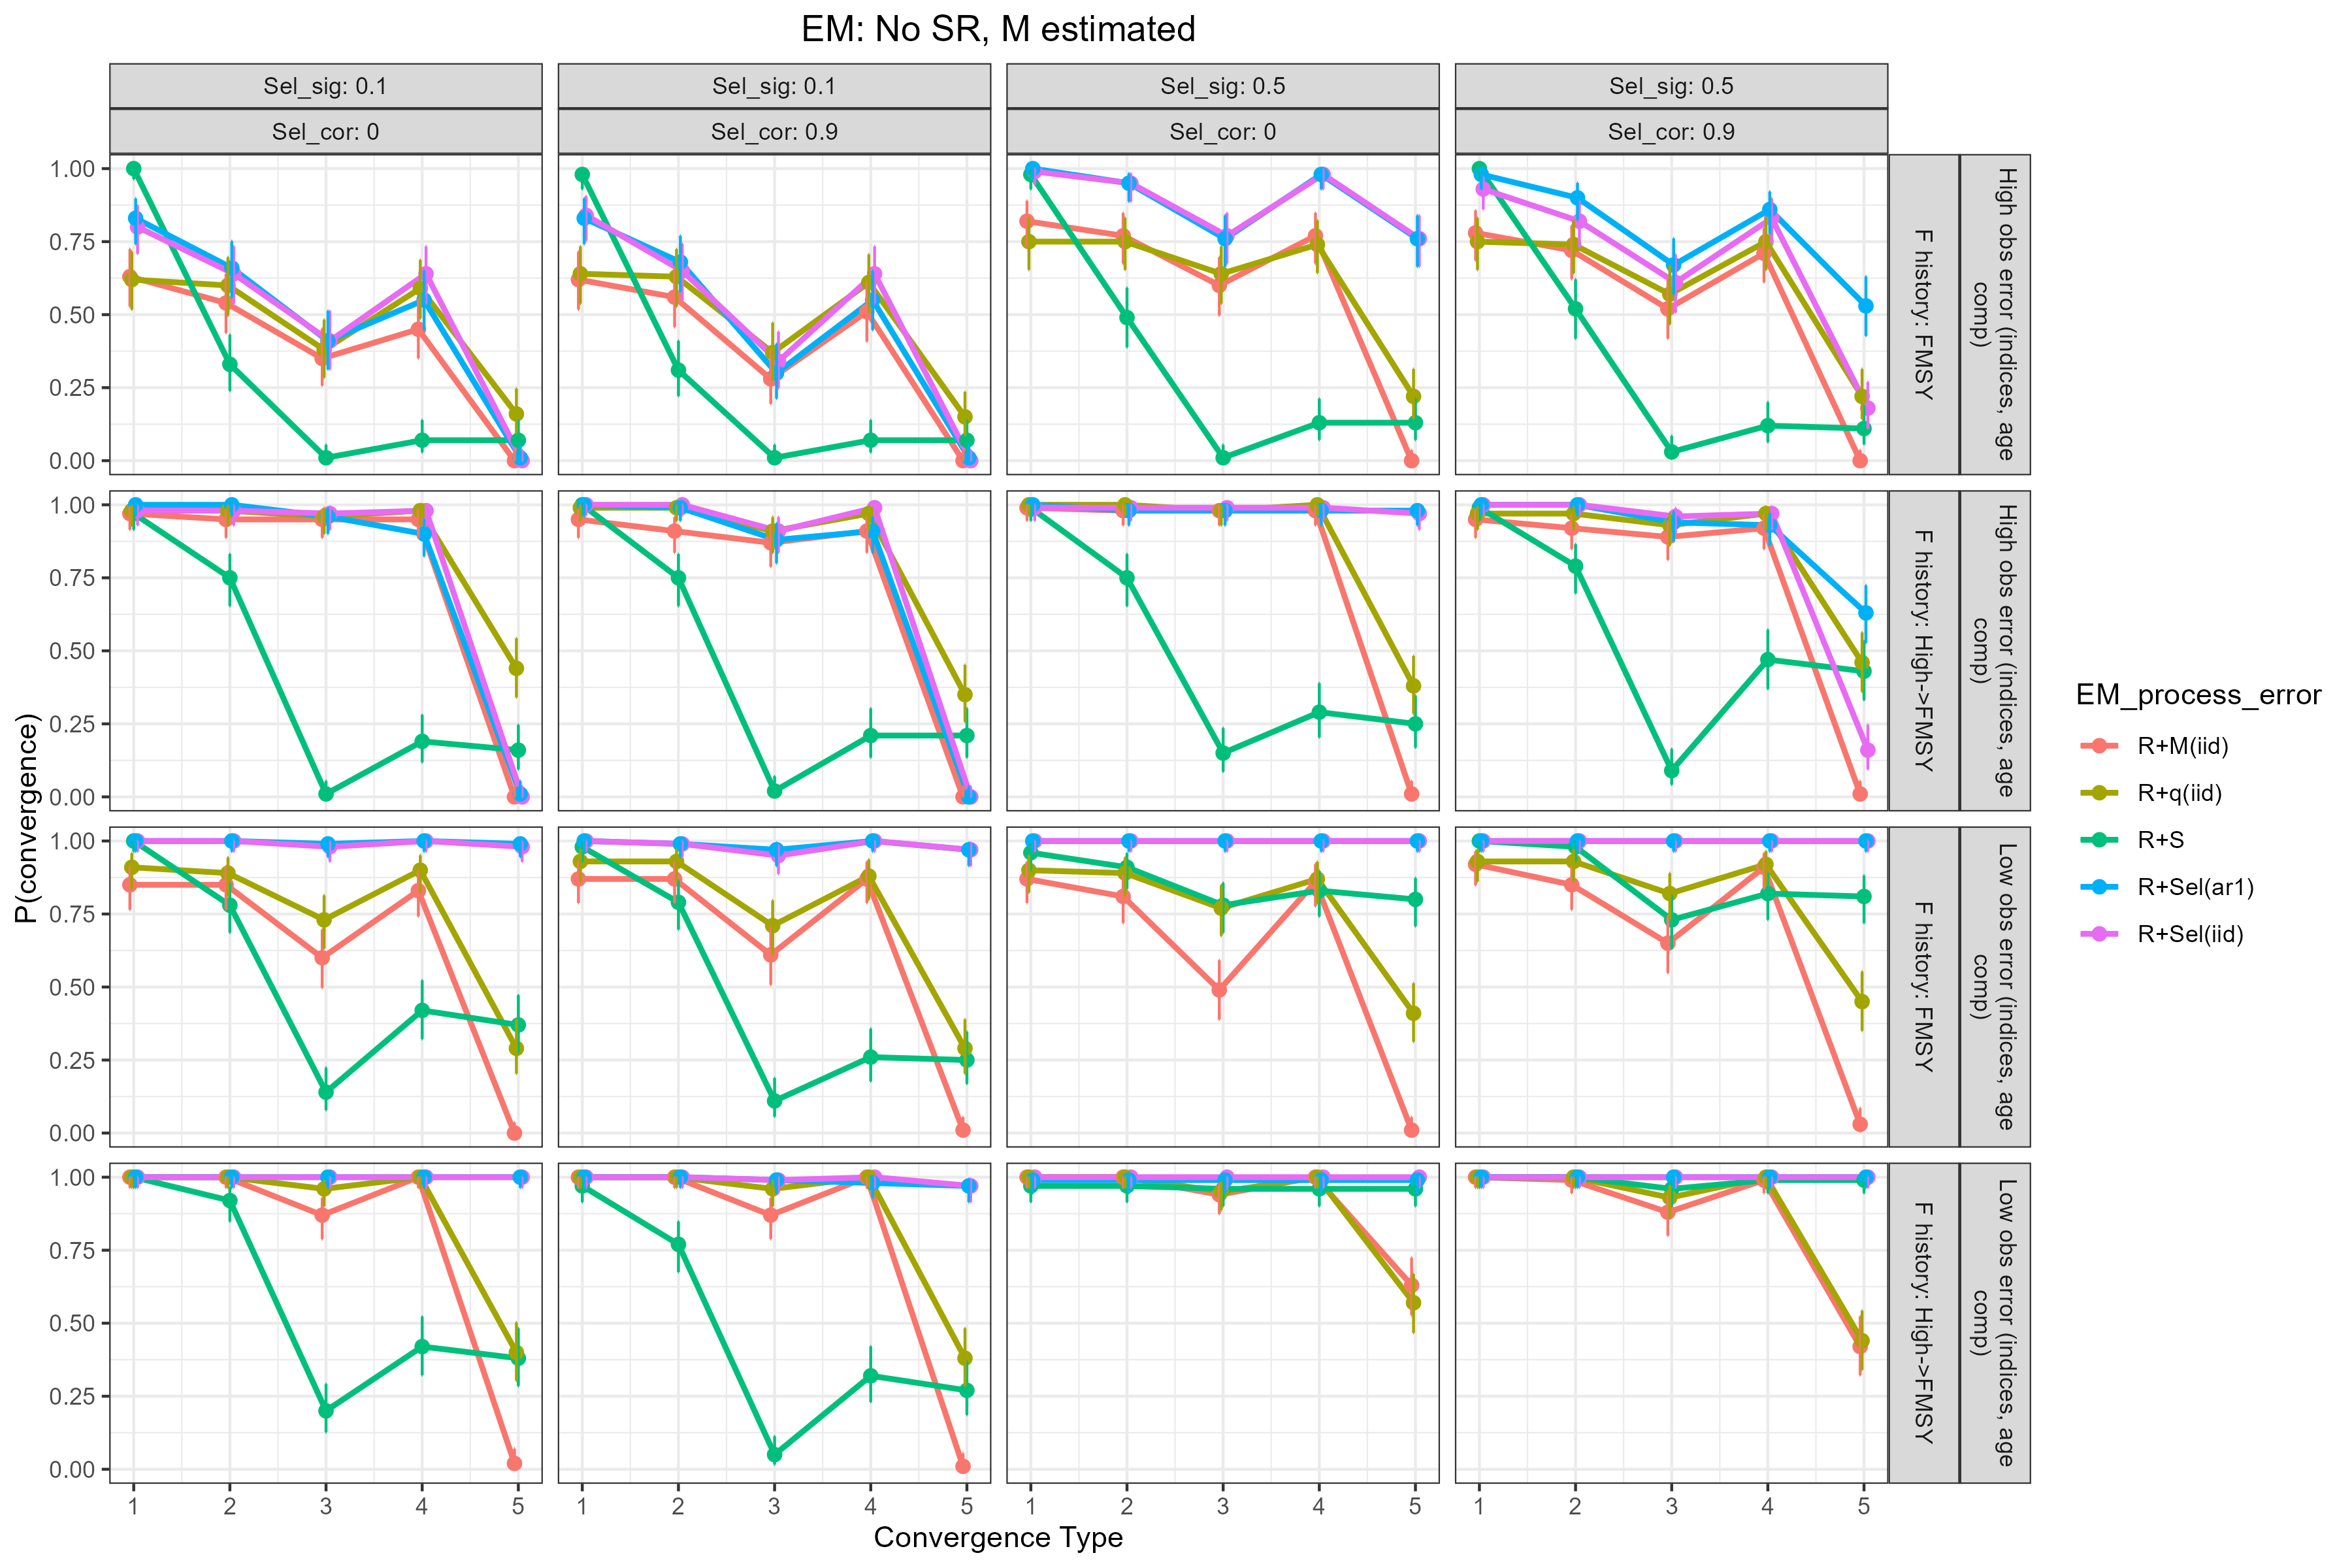
\includegraphics[width = \textwidth]{Sel_om_p_convergence_meanR_M_estimated.png}
\end{center}
\end{figure}
\end{landscape}

\begin{landscape}
\begin{figure}
\caption{Probability of each type of convergence of estimating models with alternative process error assumptions for operating models that have process error structure R+Sel. vertical lines represent 95\% confidence intervals. All estimating models estimate a Beverton-Holt stock-recruit relationship and and M is fixed at the true value.}\label{Sel_om_em_BH_MF_convergence}
\begin{center}
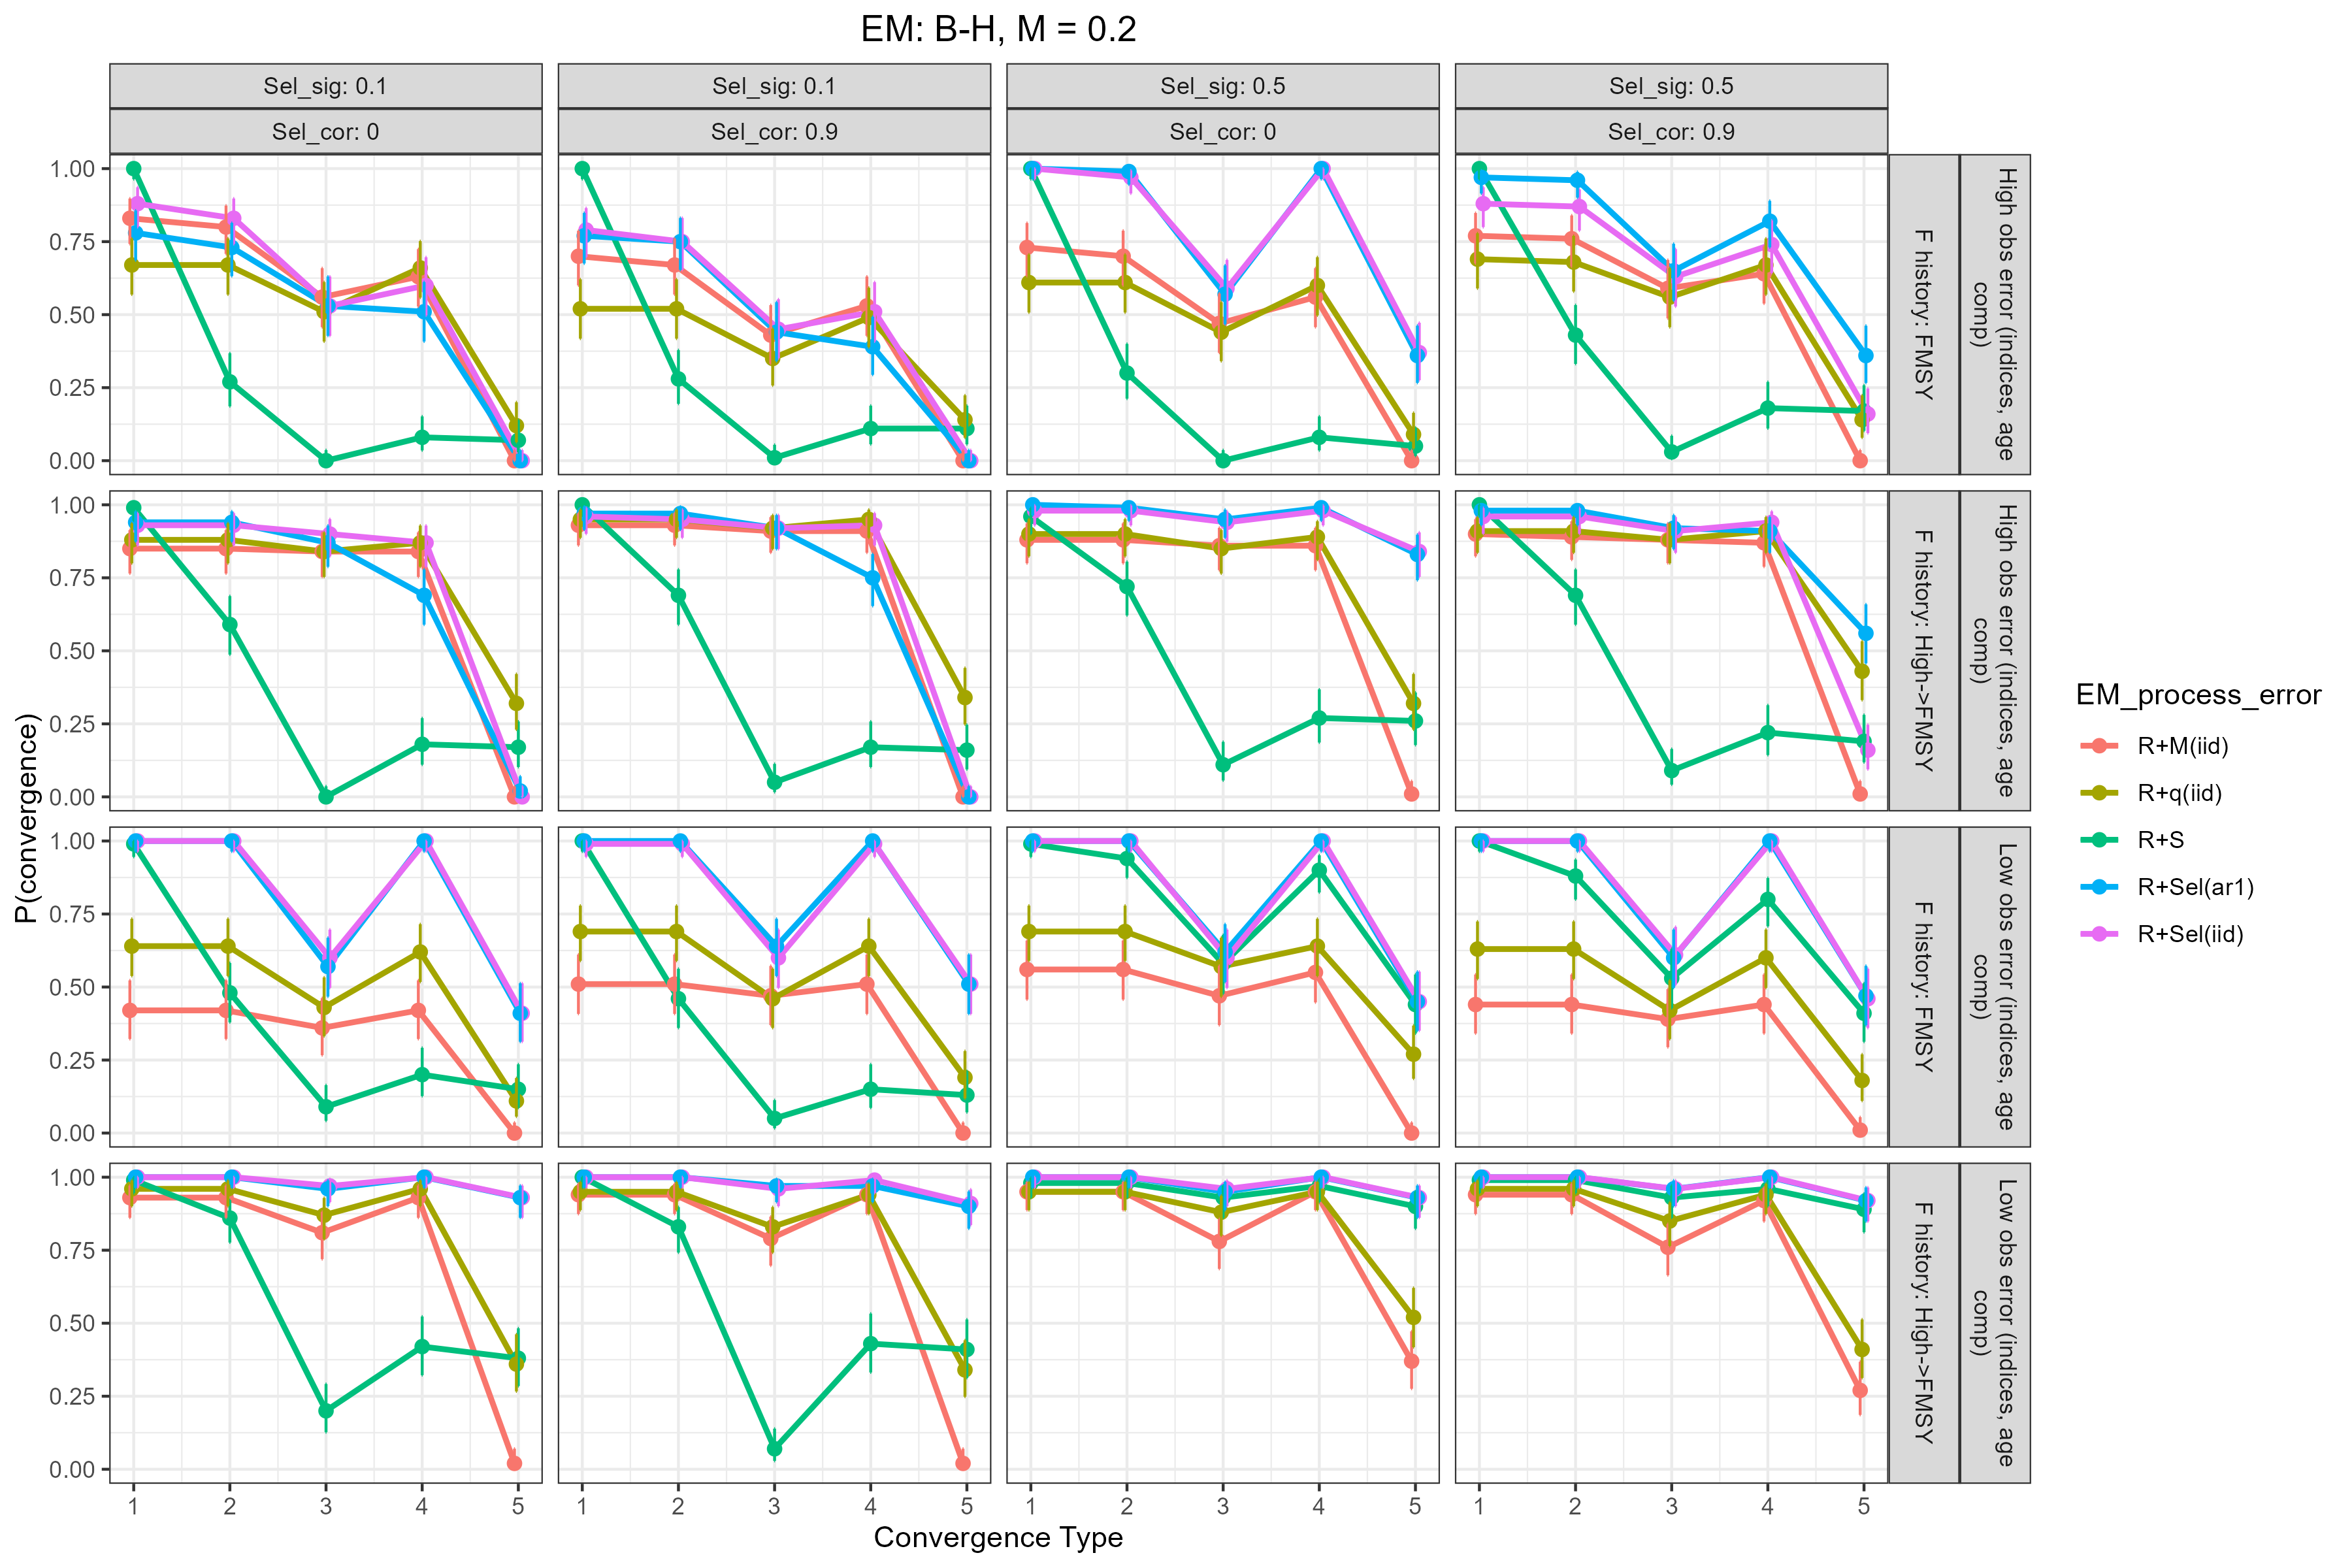
\includegraphics[width = \textwidth]{Sel_om_p_convergence_BH_M_fixed.png}
\end{center}
\end{figure}
\end{landscape}

\begin{landscape}
\begin{figure}
\caption{Probability of each type of convergence of estimating models with alternative process error assumptions for operating models that have process error structure R+Sel. vertical lines represent 95\% confidence intervals. All estimating models estimate a Beverton-Holt stock-recruit relationship and and M is estimated.}\label{Sel_om_em_BH_ME_convergence}
\begin{center}
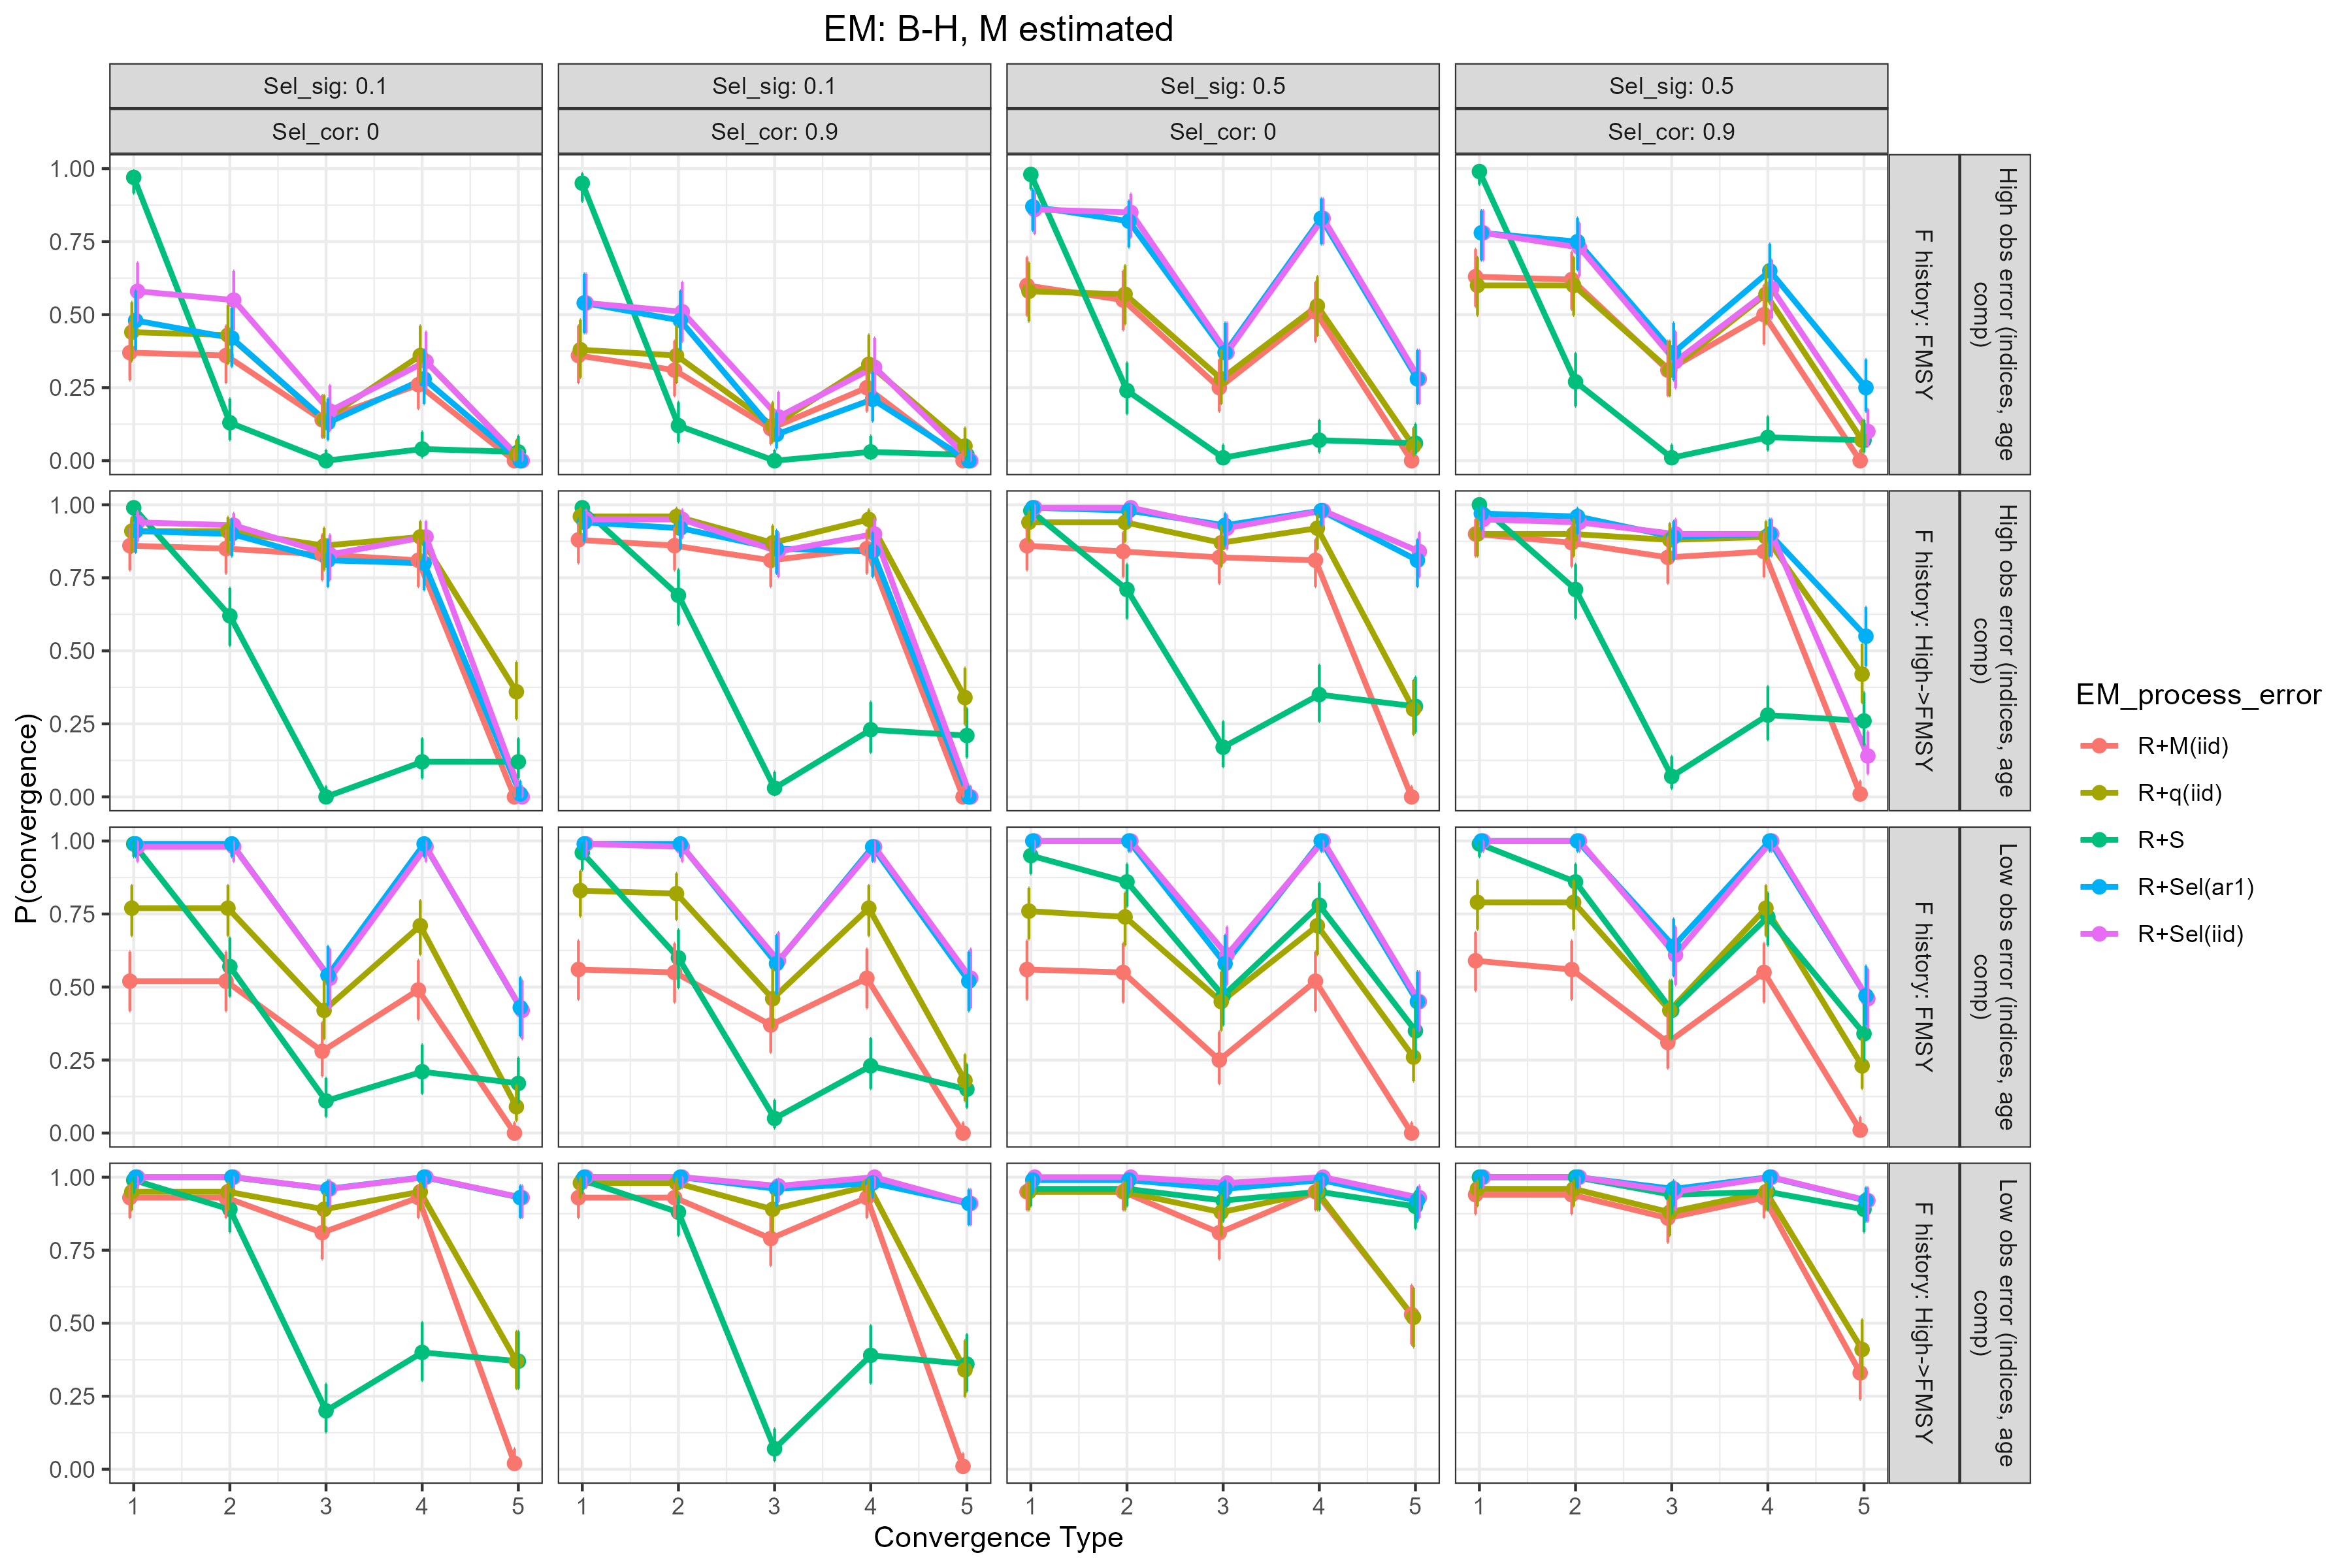
\includegraphics[width = \textwidth]{Sel_om_p_convergence_BH_M_estimated.png}
\end{center}
\end{figure}
\end{landscape}

\hypertarget{rq-operating-models}{%
\subsubsection*{R+q operating models}\label{rq-operating-models}}
\addcontentsline{toc}{subsubsection}{R+q operating models}

Figures \ref{q_om_em_R_MF_convergence} to
\ref{q_om_em_BH_ME_convergence}

\begin{landscape}
\begin{figure}
\caption{Probability of each type of convergence of estimating models with alternative process error assumptions for operating models that have process error structure R+q. vertical lines represent 95\% confidence intervals. All estimating models estimate mean recruitment rather than a stock-recruit relationship and and M is fixed at the true value.}\label{q_om_em_R_MF_convergence}
\begin{center}
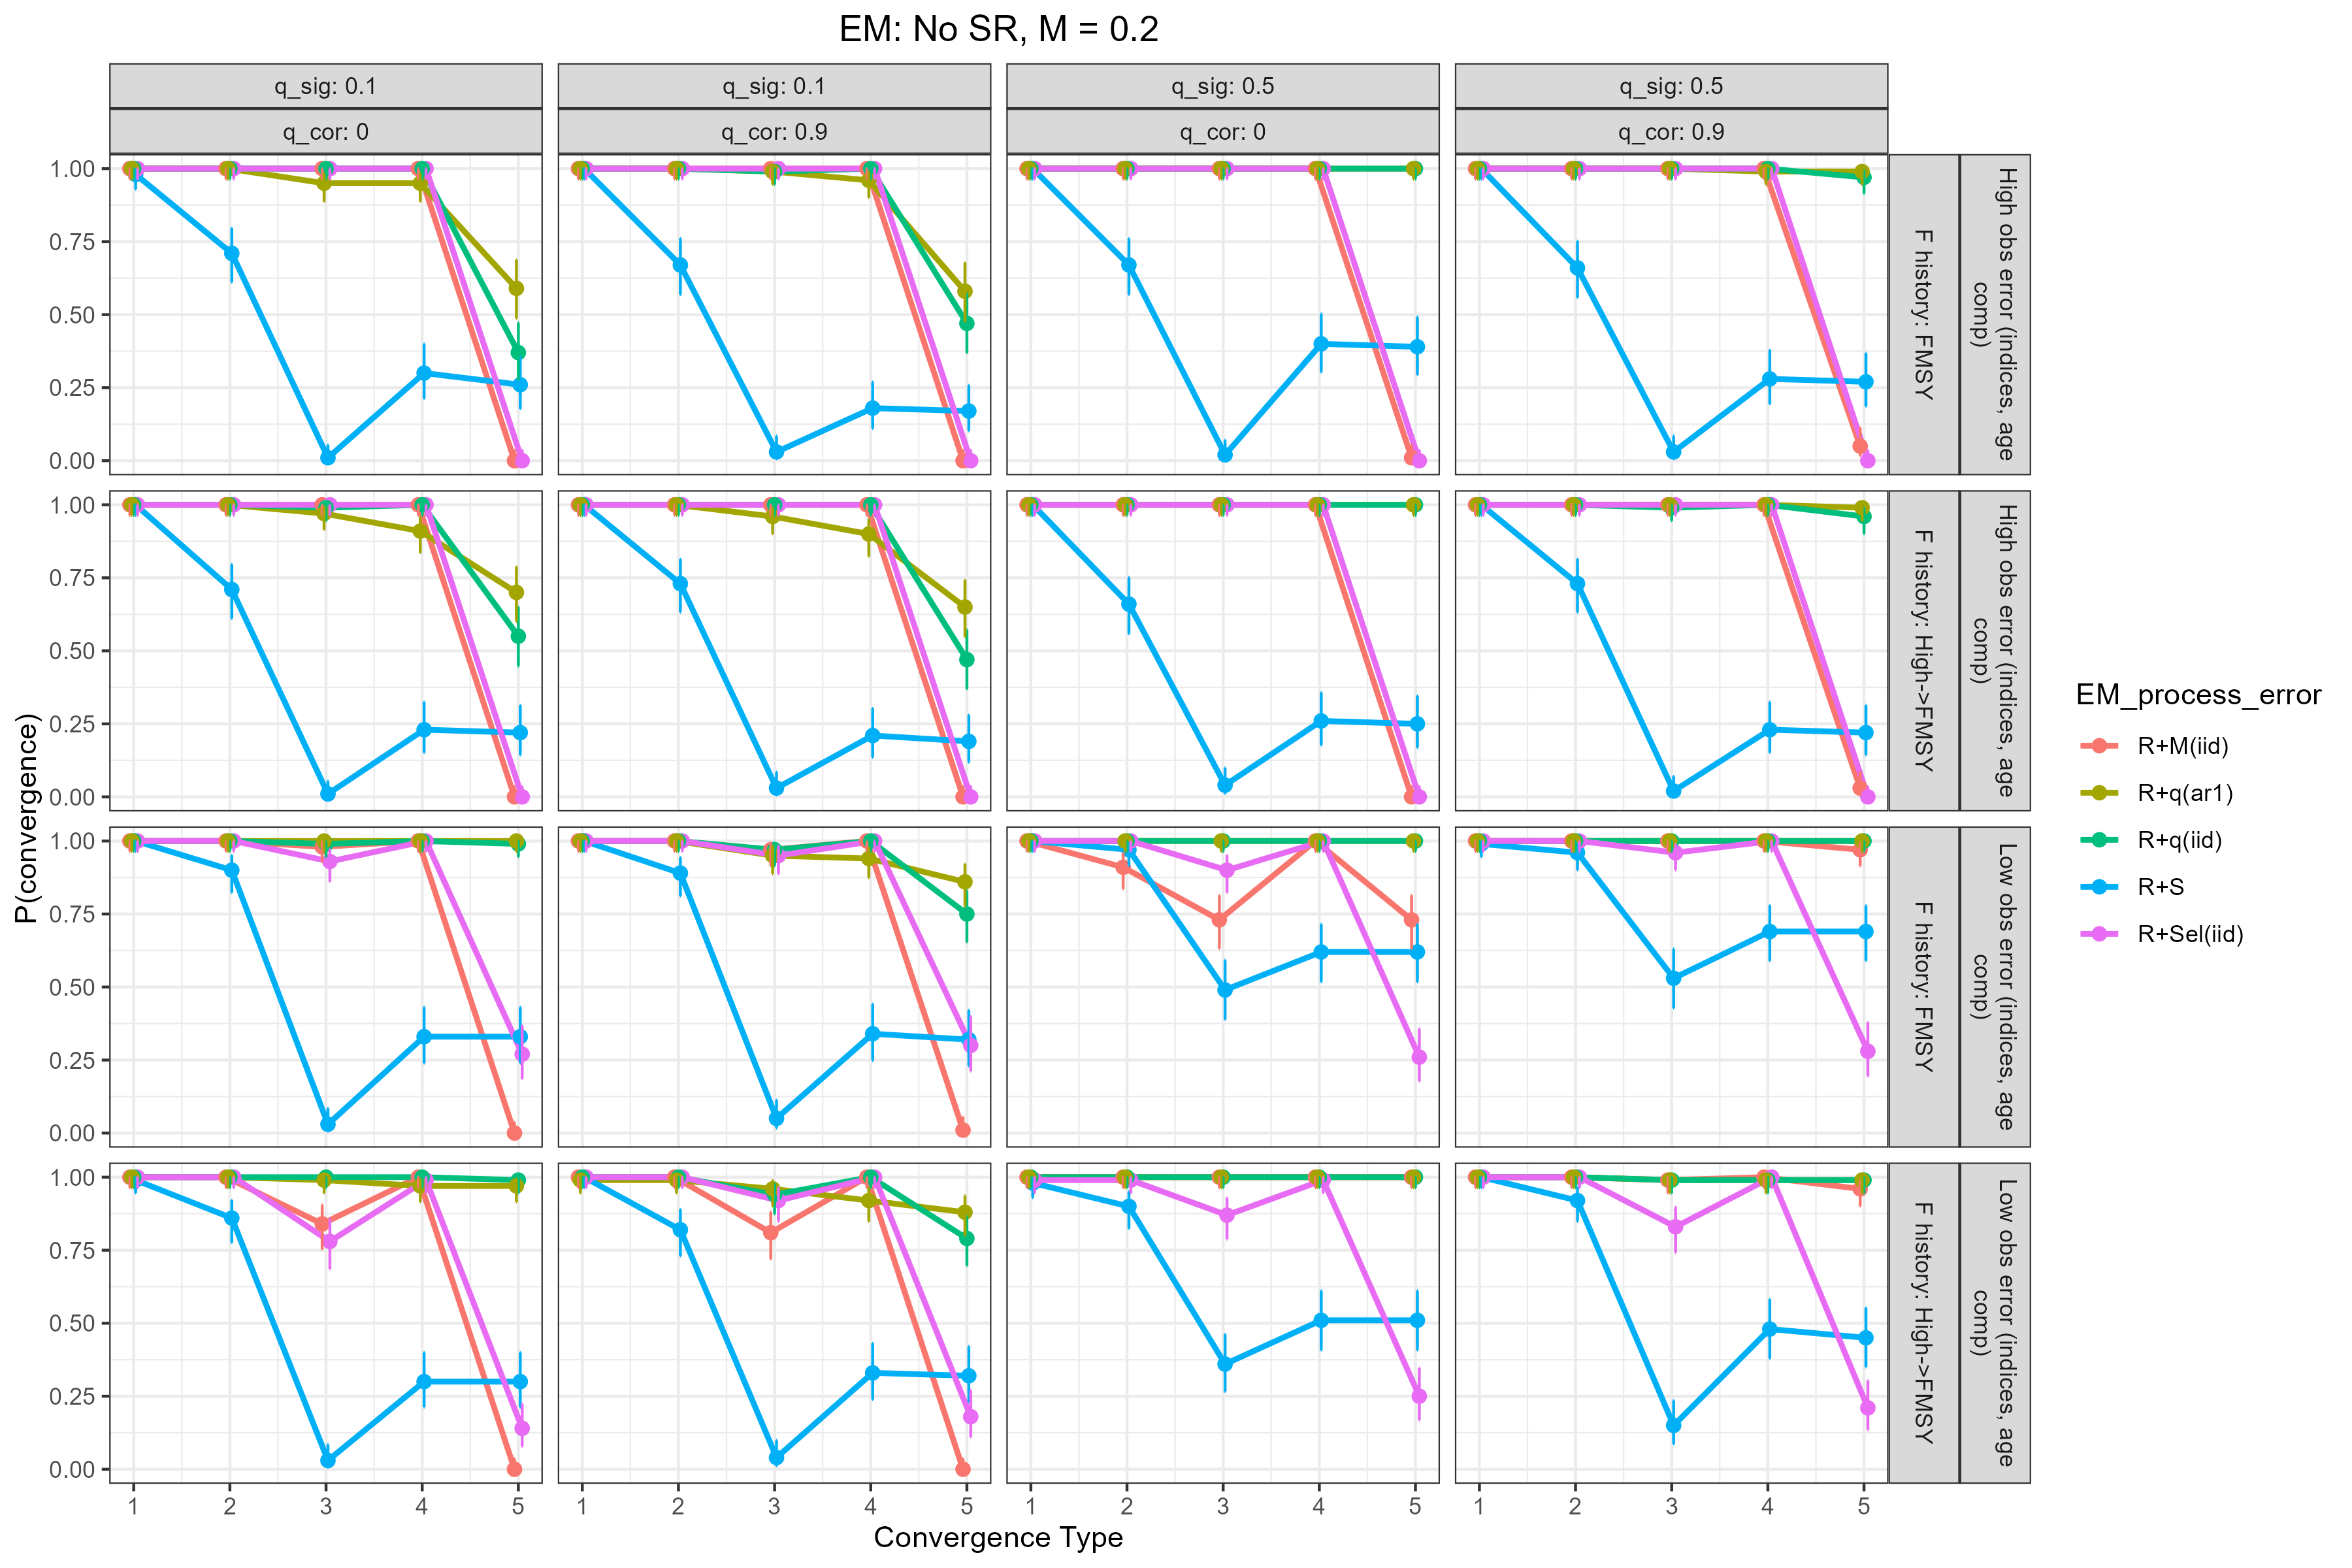
\includegraphics[width = \textwidth]{q_om_p_convergence_meanR_M_fixed.png}
\end{center}
\end{figure}
\end{landscape}

\begin{landscape}
\begin{figure}
\caption{Probability of each type of convergence of estimating models with alternative process error assumptions for operating models that have process error structure R+q. vertical lines represent 95\% confidence intervals. All estimating models estimate mean recruitment rather than a stock-recruit relationship and and M is estimated.}\label{q_om_em_R_ME_convergence}
\begin{center}
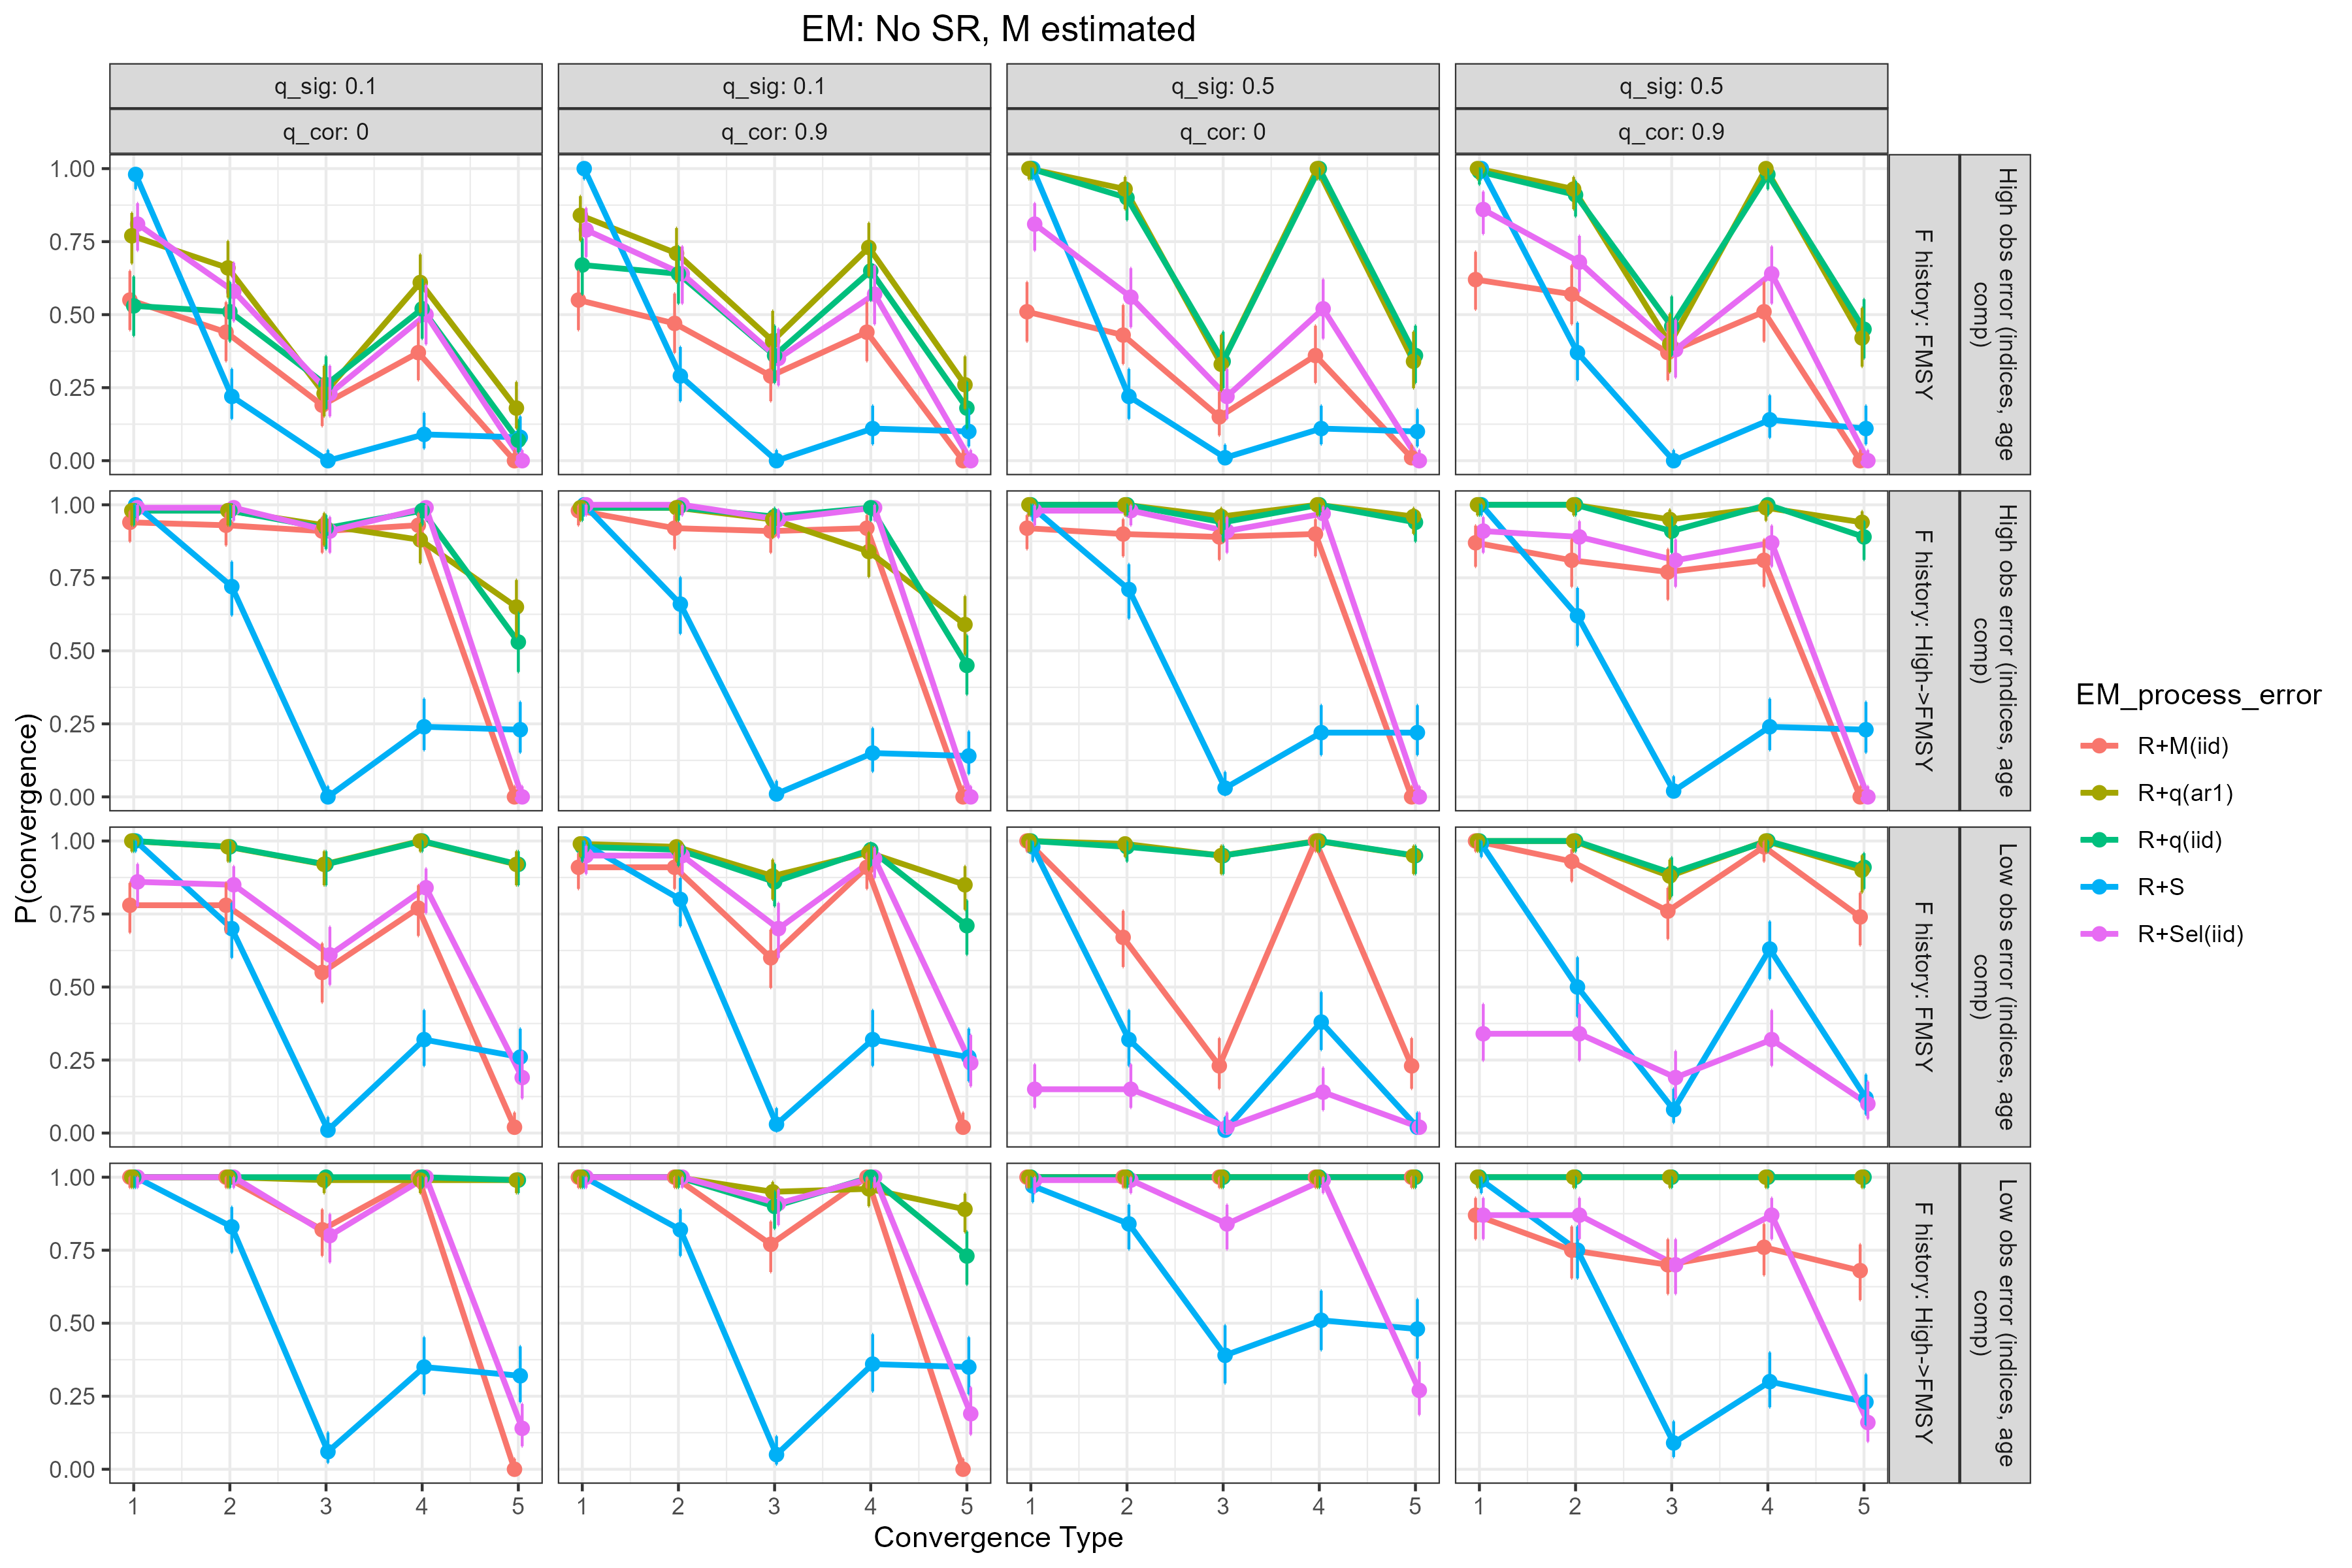
\includegraphics[width = \textwidth]{q_om_p_convergence_meanR_M_estimated.png}
\end{center}
\end{figure}
\end{landscape}

\begin{landscape}
\begin{figure}
\caption{Probability of each type of convergence of estimating models with alternative process error assumptions for operating models that have process error structure R+q. vertical lines represent 95\% confidence intervals. All estimating models estimate a Beverton-Holt stock-recruit relationship and and M is fixed at the true value.}\label{q_om_em_BH_MF_convergence}
\begin{center}
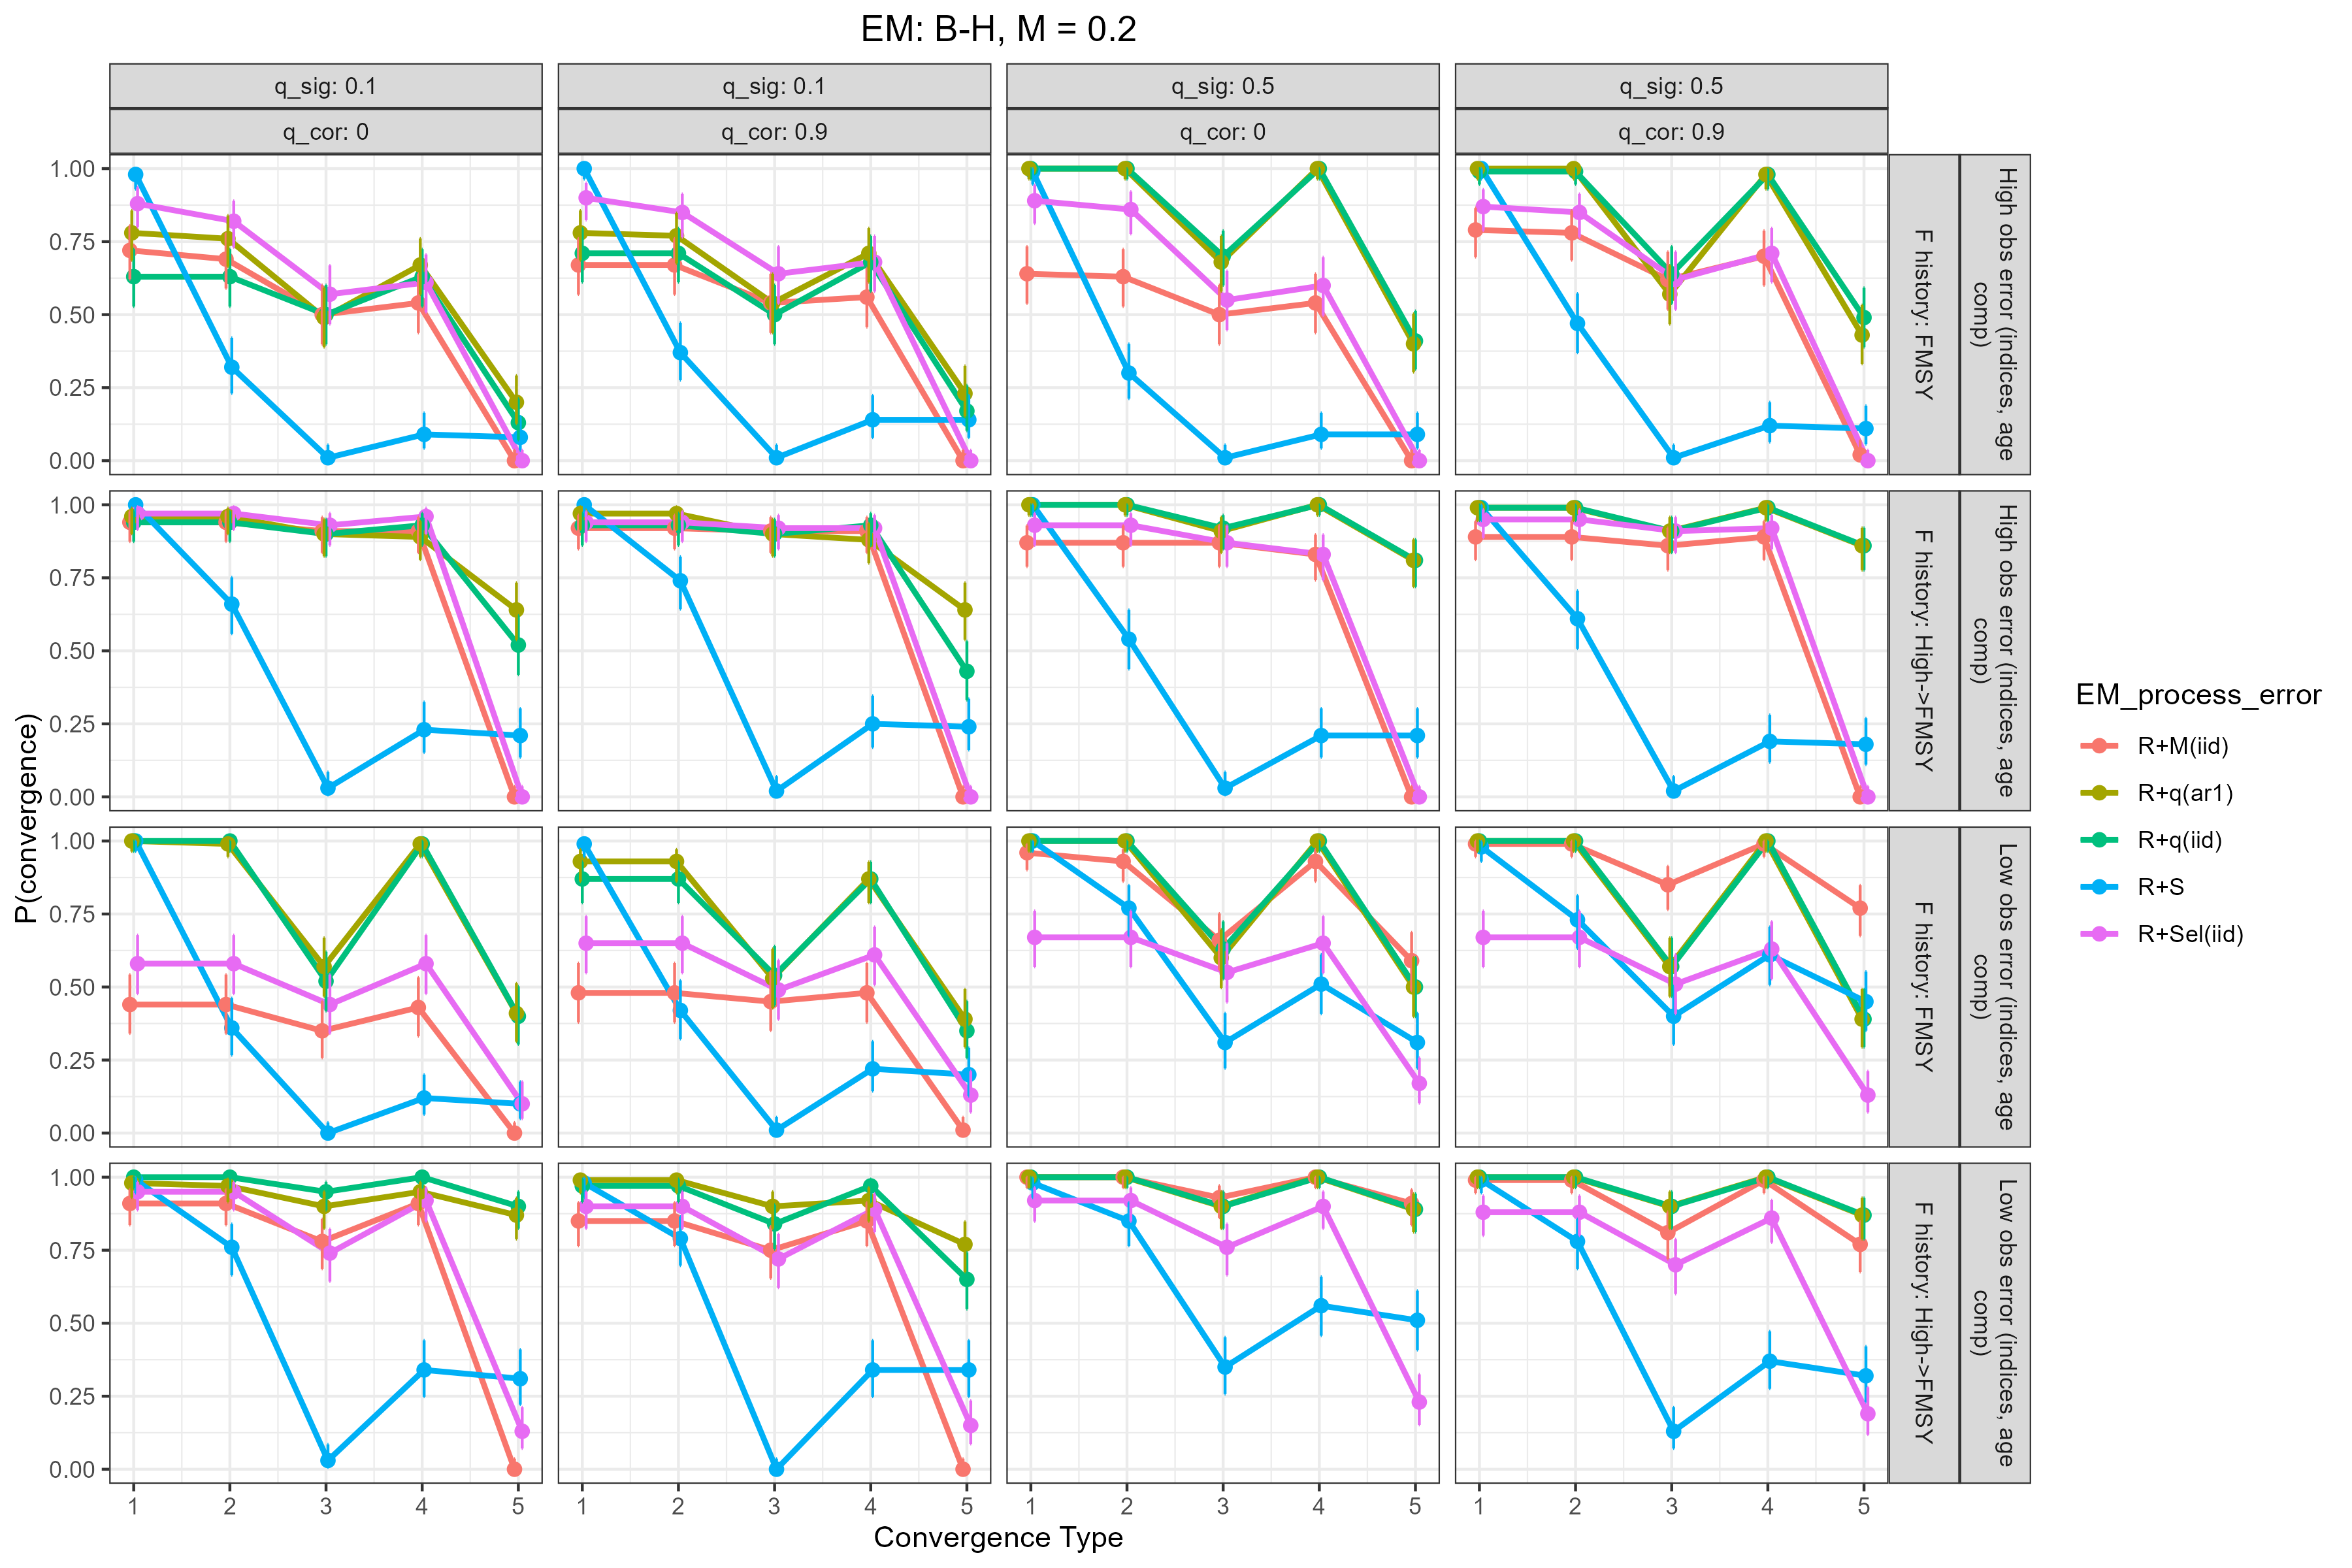
\includegraphics[width = \textwidth]{q_om_p_convergence_BH_M_fixed.png}
\end{center}
\end{figure}
\end{landscape}

\begin{landscape}
\begin{figure}
\caption{Probability of each type of convergence of estimating models with alternative process error assumptions for operating models that have process error structure R+q. vertical lines represent 95\% confidence intervals. All estimating models estimate a Beverton-Holt stock-recruit relationship and and M is estimated.}\label{q_om_em_BH_ME_convergence}
\begin{center}
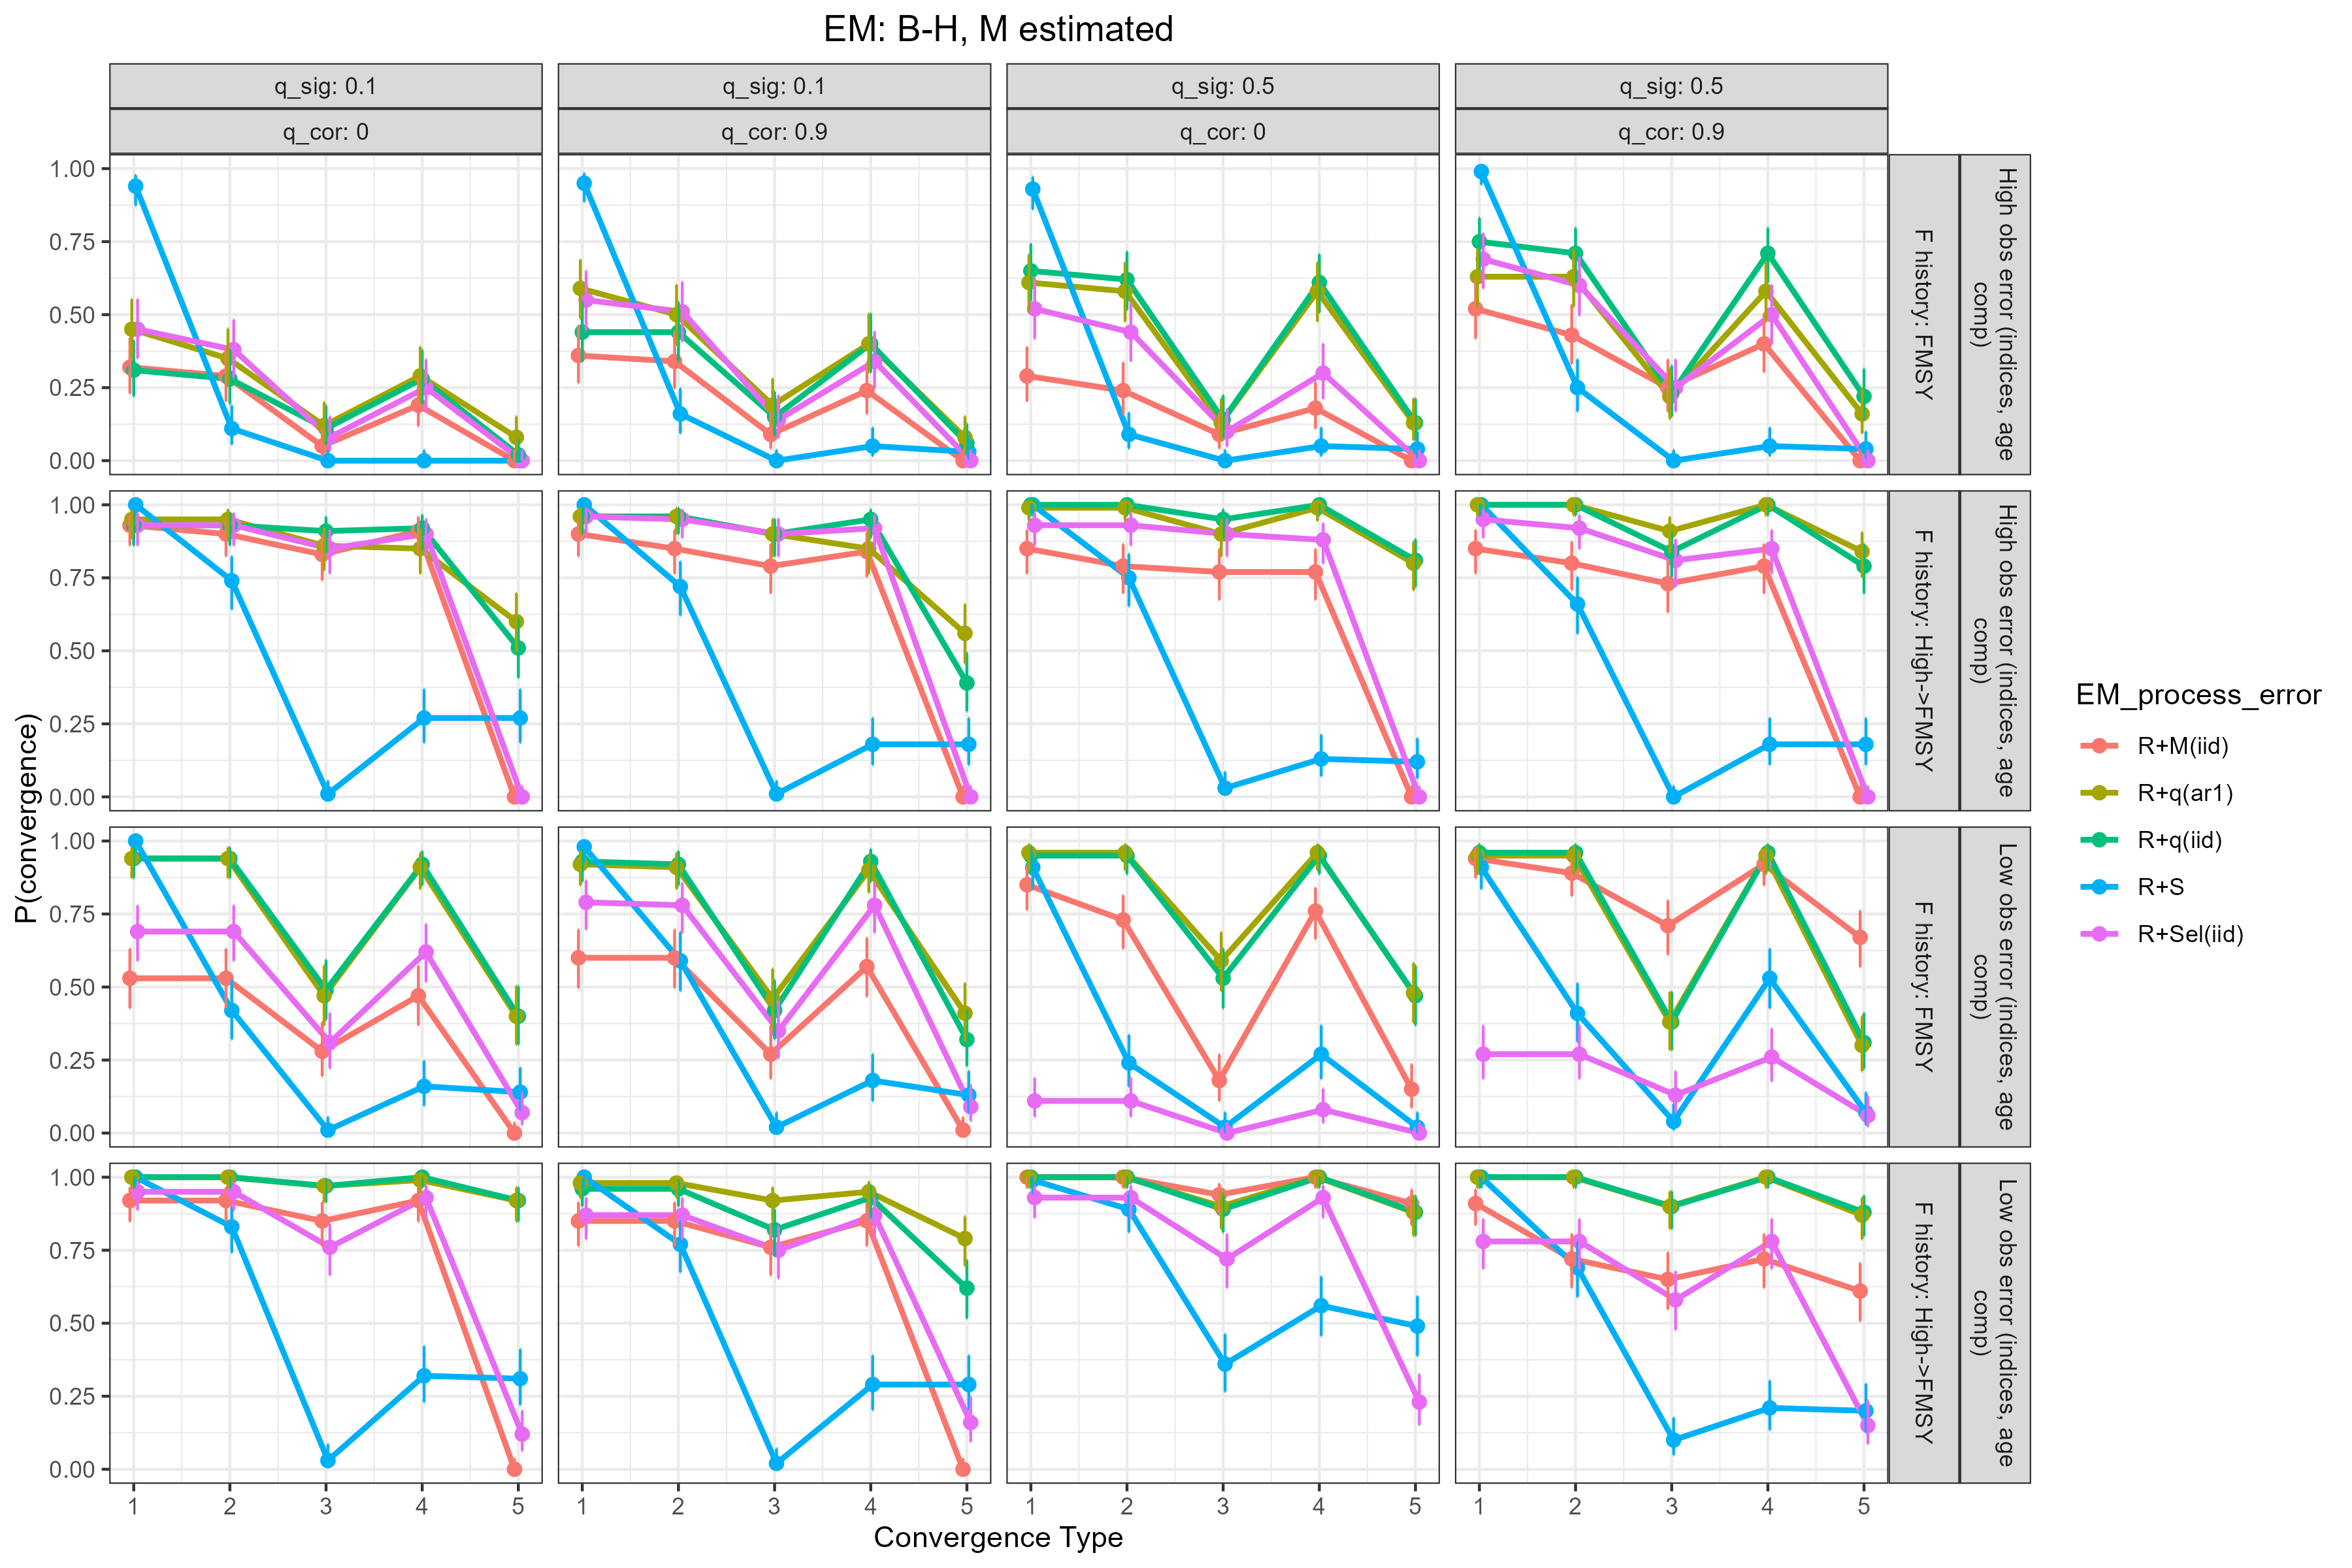
\includegraphics[width = \textwidth]{q_om_p_convergence_BH_M_estimated.png}
\end{center}
\end{figure}
\end{landscape}

\hypertarget{aic-performance-for-process-error-structure}{%
\subsection*{AIC performance for process error
structure}\label{aic-performance-for-process-error-structure}}
\addcontentsline{toc}{subsection}{AIC performance for process error
structure}

\hypertarget{r-rs-operating-models-1}{%
\subsubsection*{R, R+S operating models}\label{r-rs-operating-models-1}}
\addcontentsline{toc}{subsubsection}{R, R+S operating models}

Figures \ref{naa_om_proportion_best_aic_R_MF} to
\ref{naa_om_proportion_best_aic_SR_ME}

\begin{landscape}
\begin{figure}
\caption{Proportion of simulated data sets from OMs with R and R+S process errors where fitted estimating models had lowest marginal AIC. All estimating models estimate mean recruitment rather than a stock-recruit relationship and and M is fixed at the true value.} \label{naa_om_proportion_best_aic_R_MF}
\begin{center}
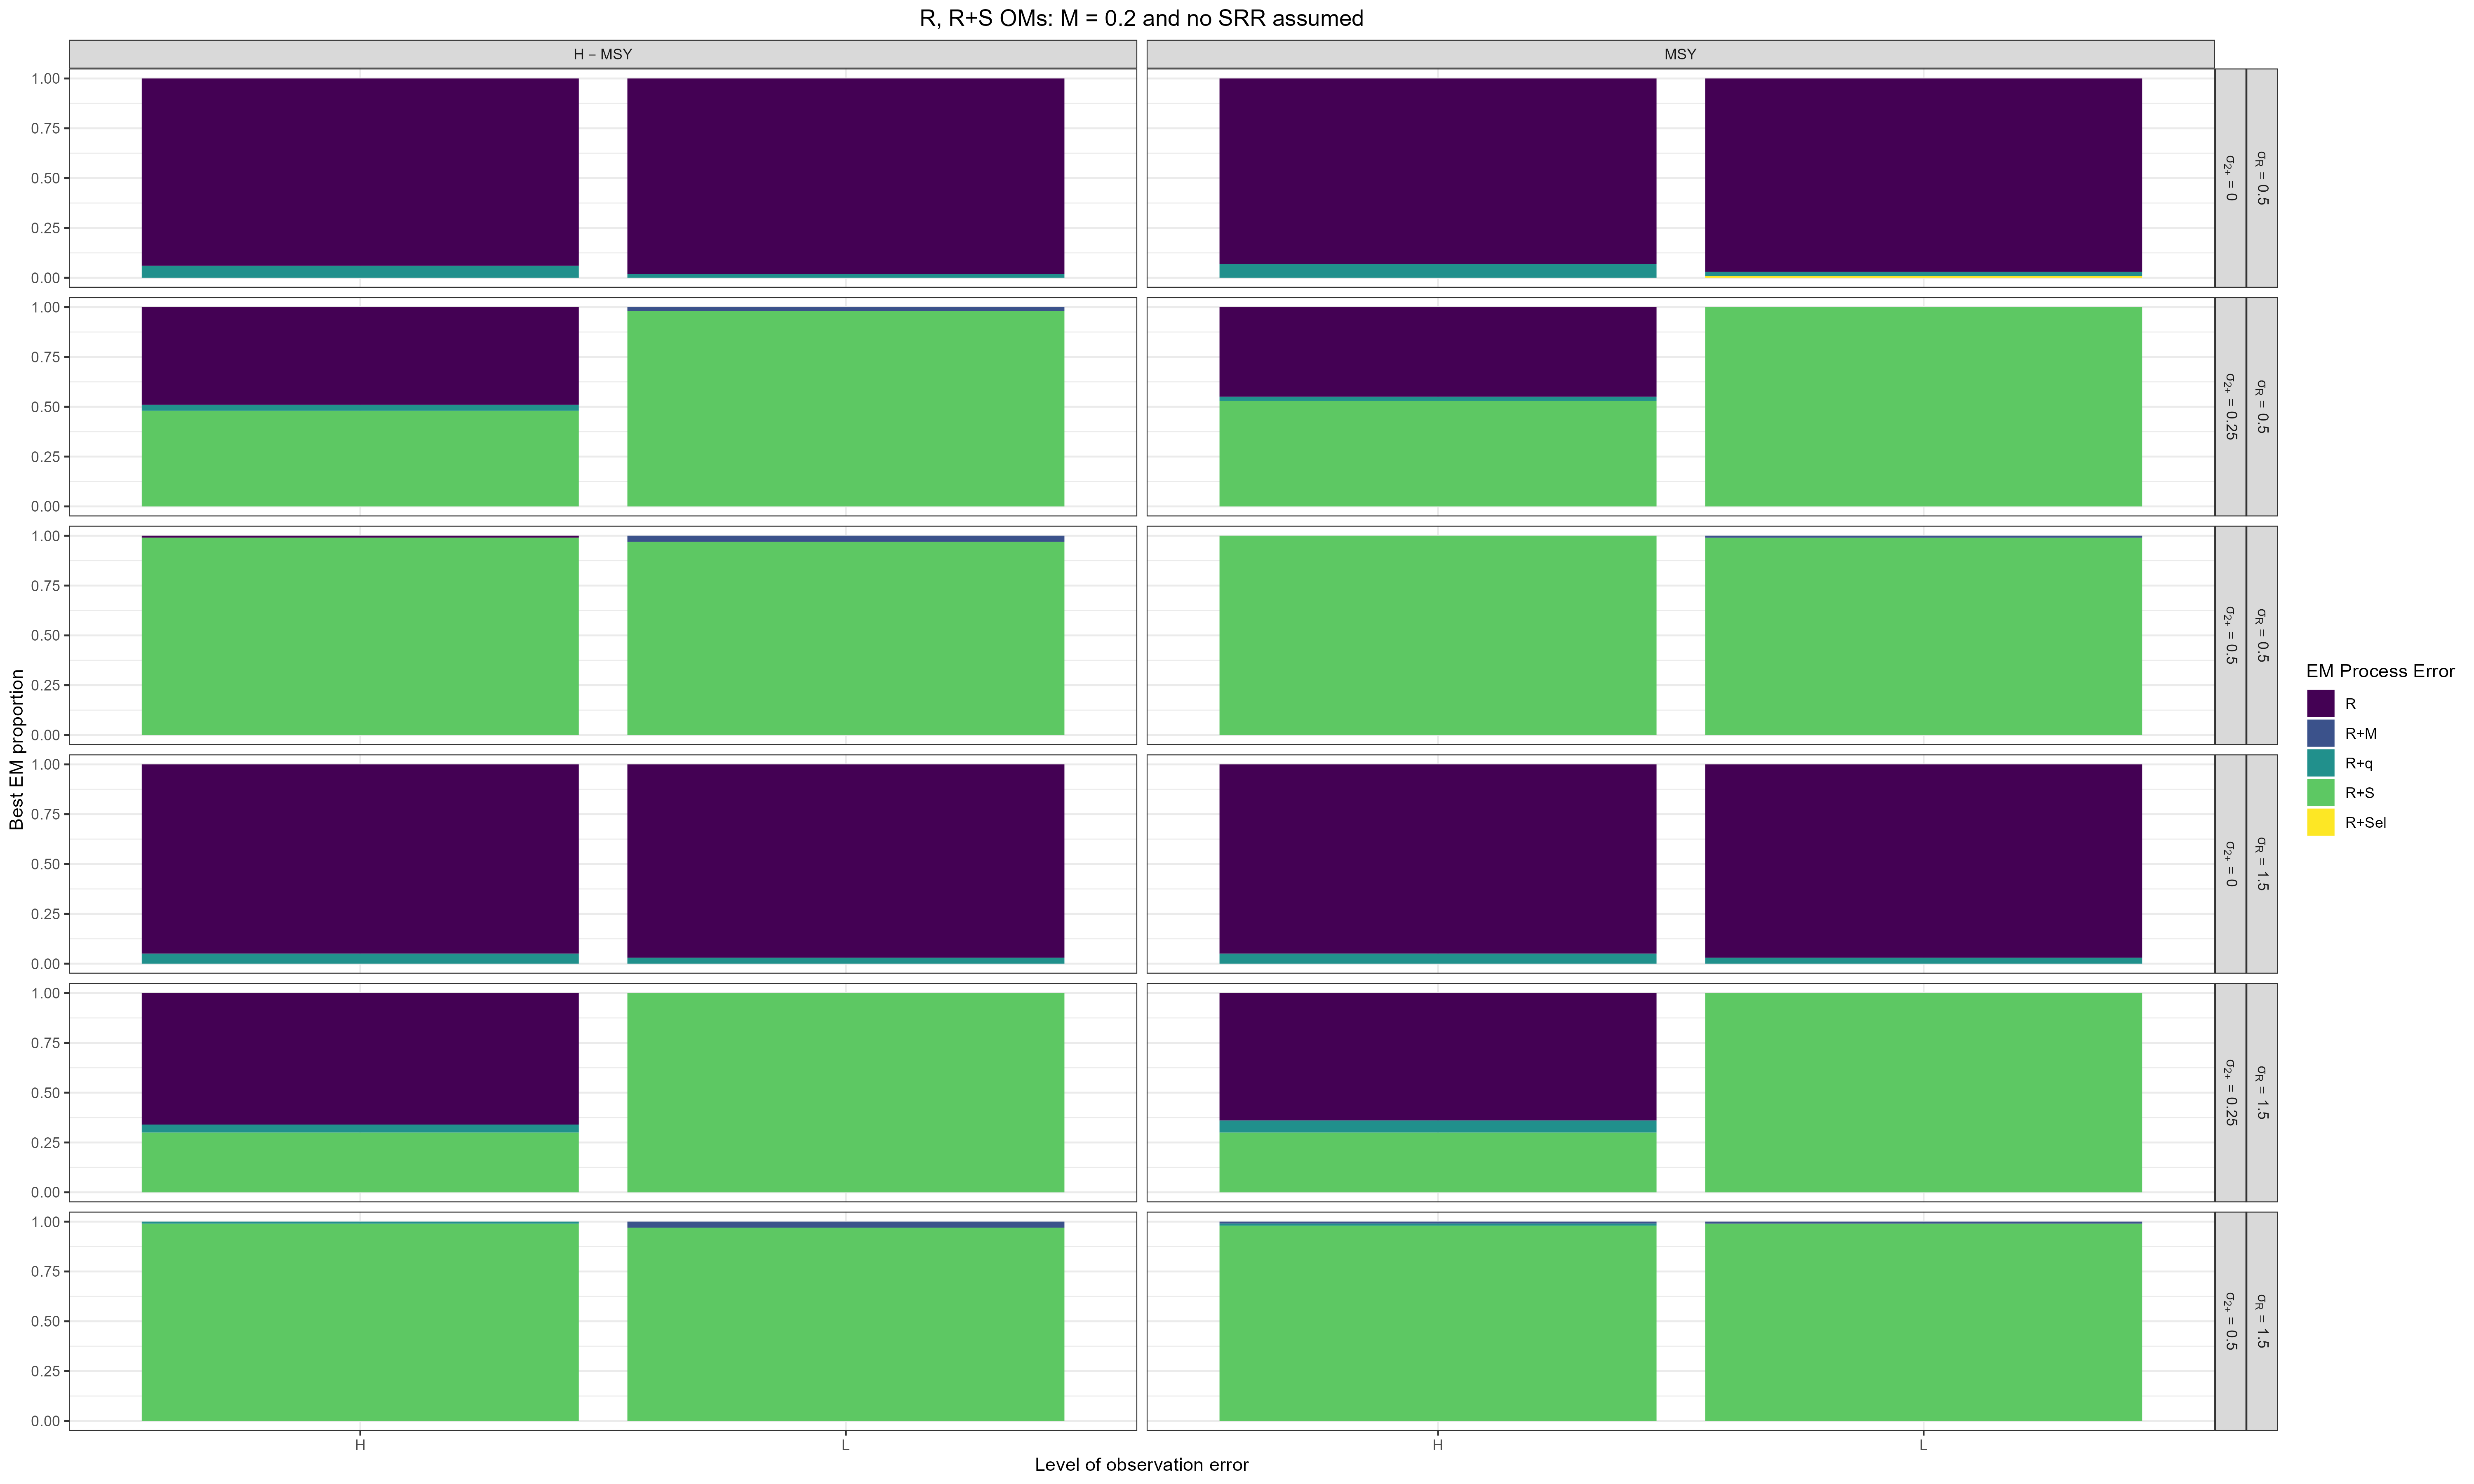
\includegraphics[width = \textwidth]{naa_om_proportion_best_aic_R_MF.png}
\end{center}
\end{figure}
\end{landscape}

\begin{landscape}
\begin{figure}
\caption{Proportion of simulated data sets from OMs with R and R+S process errors where fitted estimating models had lowest marginal AIC. All estimating models estimate mean recruitment rather than a stock-recruit relationship and and M is estimated.} \label{naa_om_proportion_best_aic_R_ME}
\begin{center}
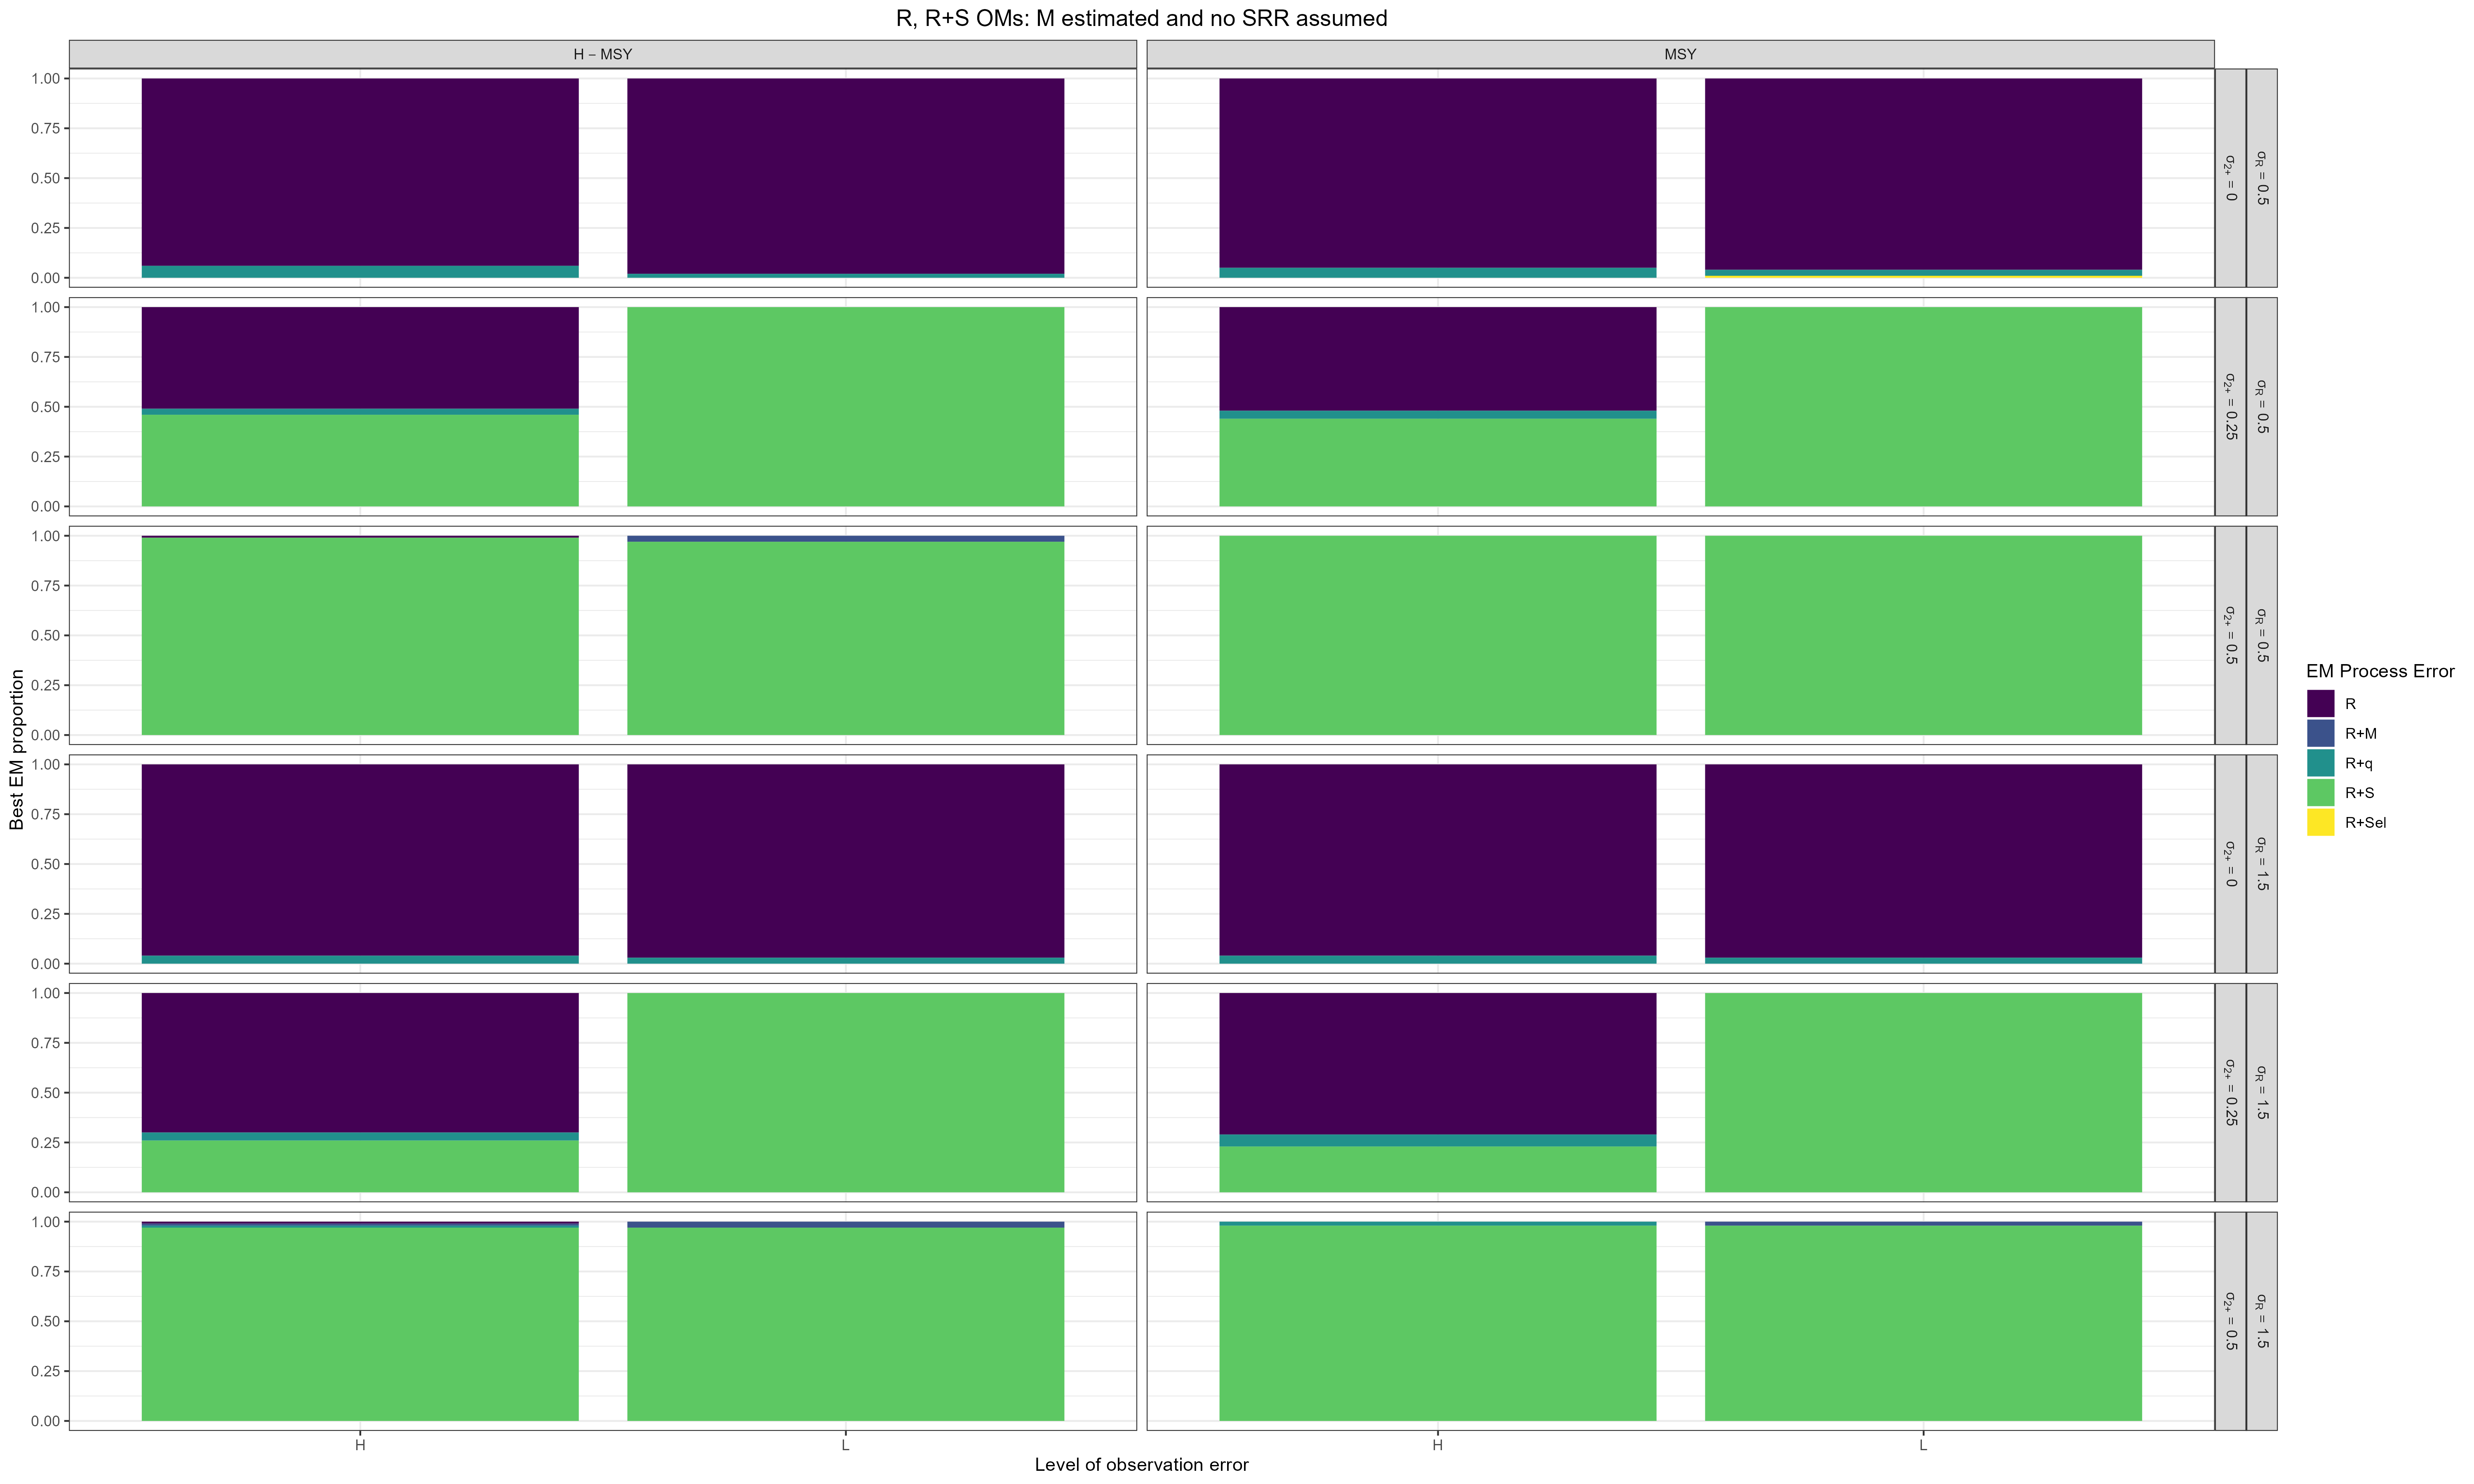
\includegraphics[width = \textwidth]{naa_om_proportion_best_aic_R_ME.png}
\end{center}
\end{figure}
\end{landscape}

\begin{landscape}
\begin{figure}
\caption{Proportion of simulated data sets from OMs with R and R+S process errors where fitted estimating models had lowest marginal AIC. All estimating models estimate a stock-recruit relationship and and M is fixed at the true value.} \label{naa_om_proportion_best_aic_SR_MF}
\begin{center}
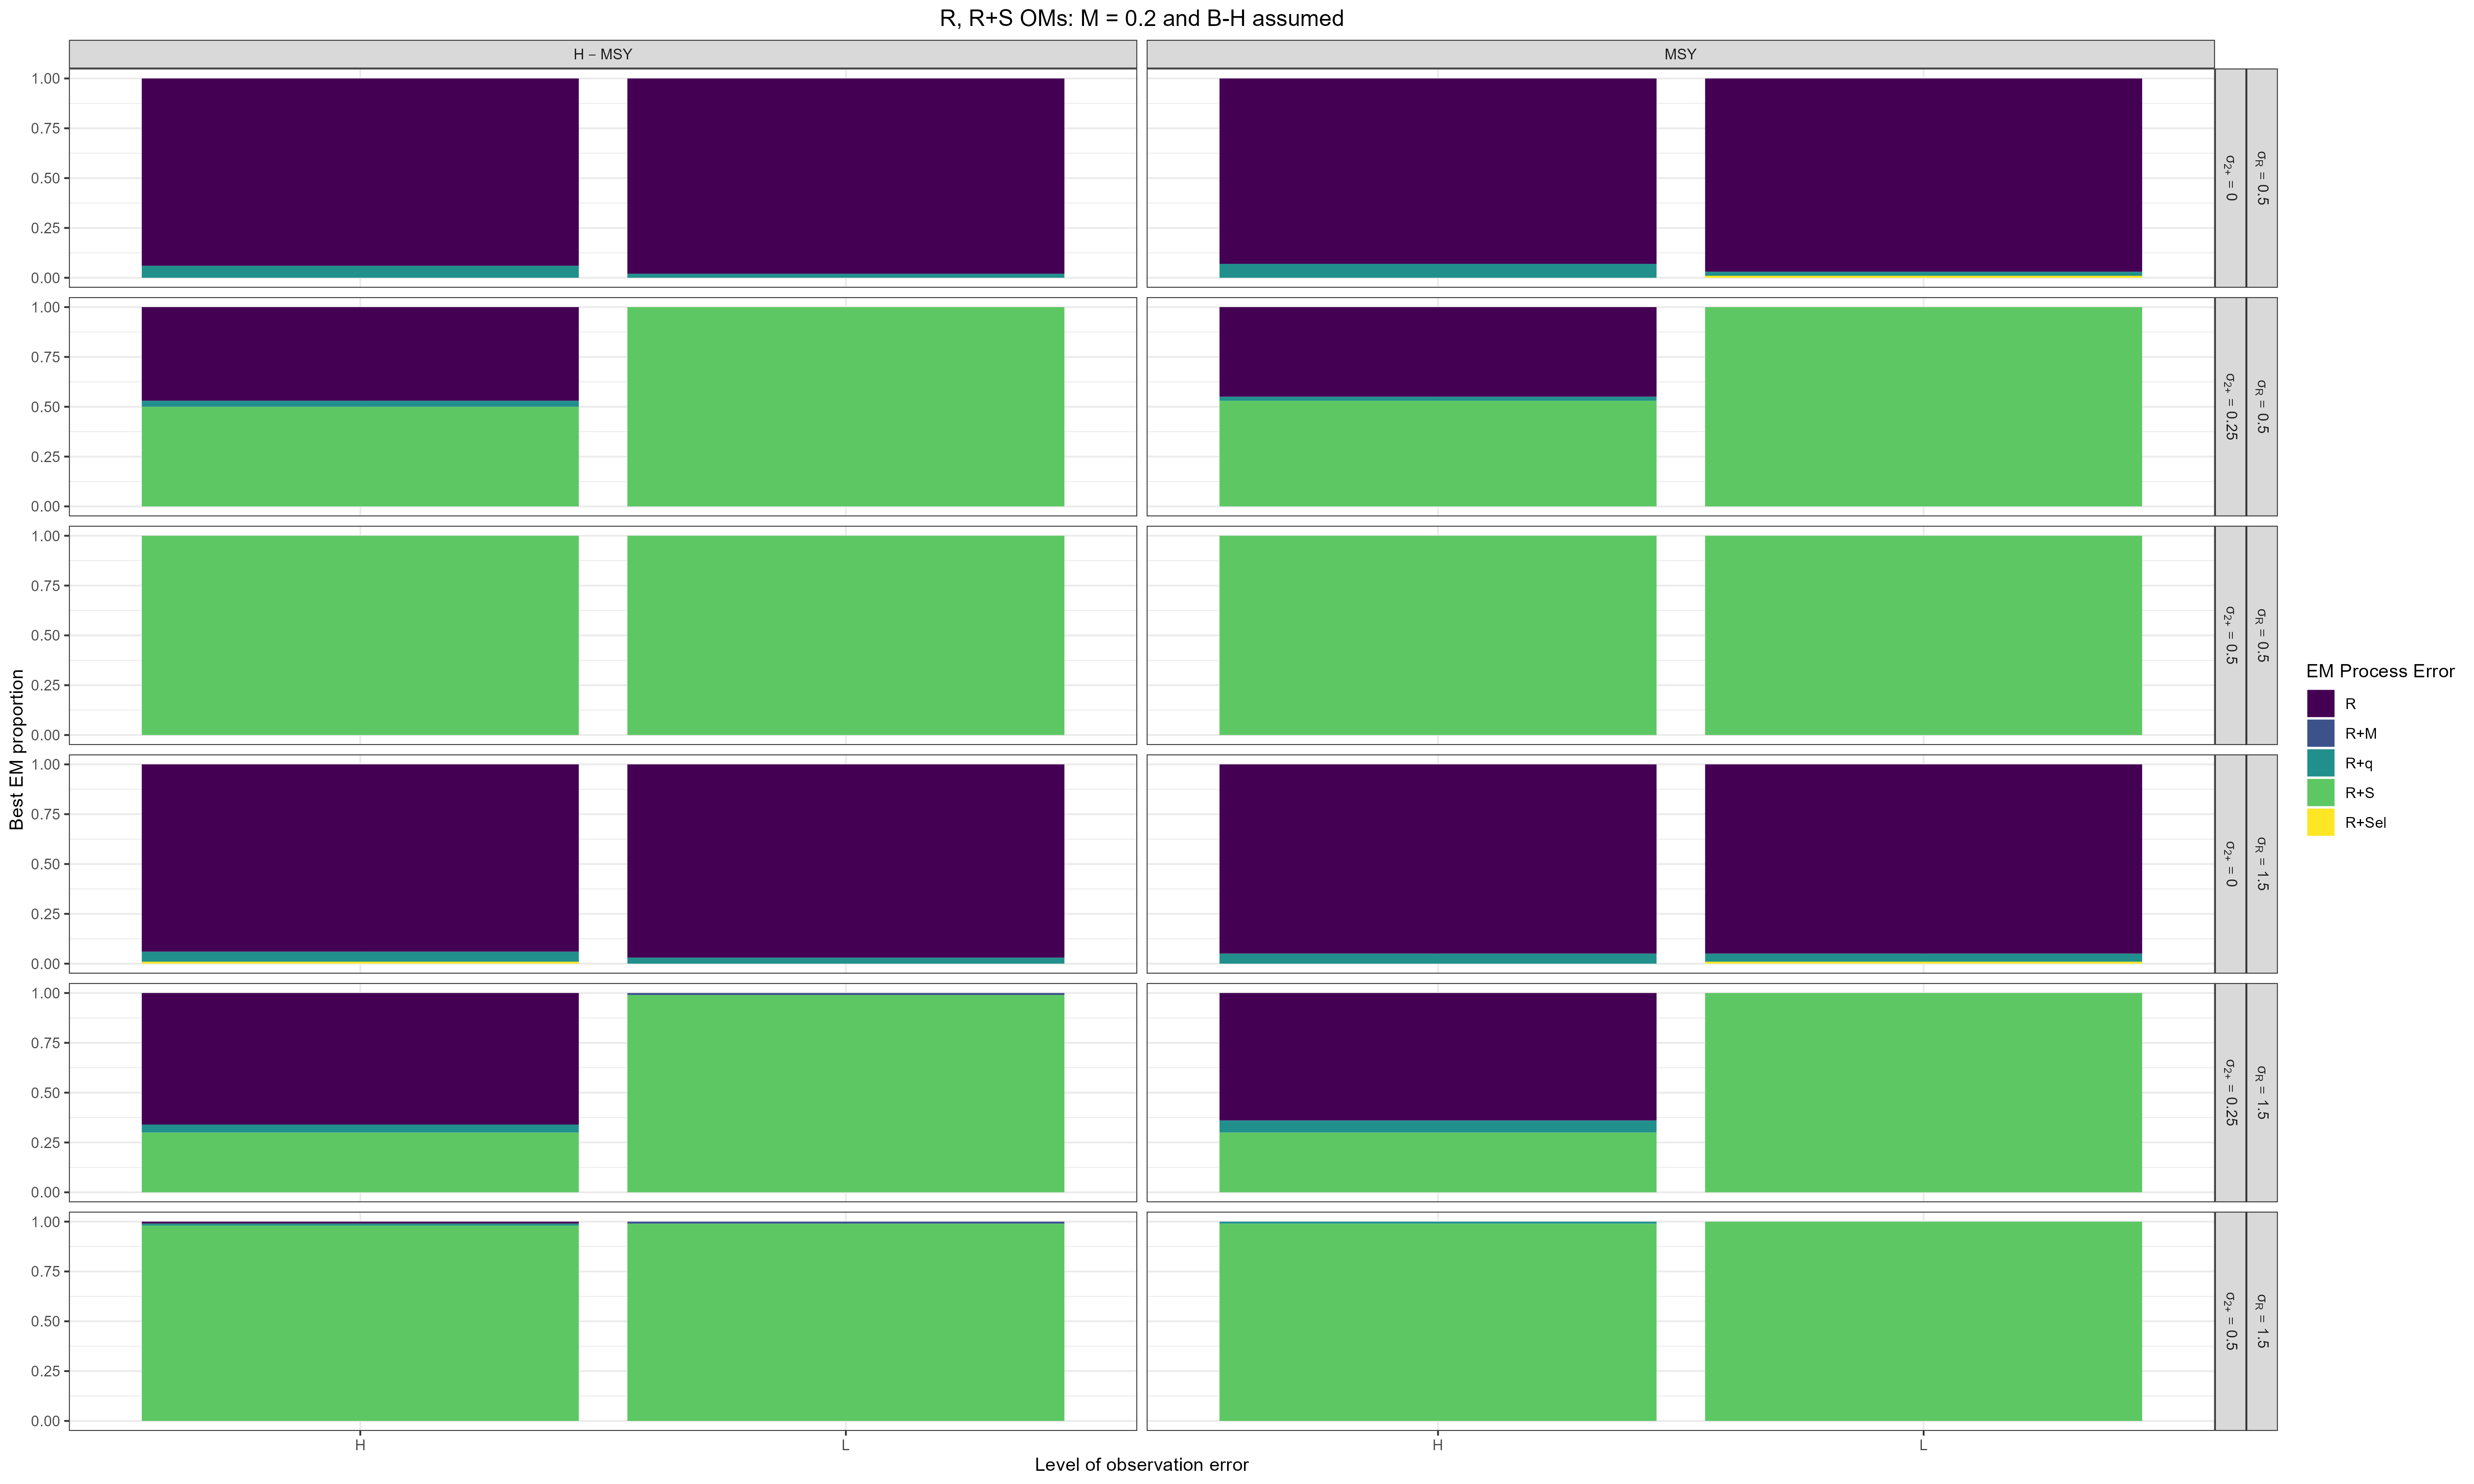
\includegraphics[width = \textwidth]{naa_om_proportion_best_aic_SR_MF.png}
\end{center}
\end{figure}
\end{landscape}

\begin{landscape}
\begin{figure}
\caption{Proportion of simulated data sets from OMs with R and R+S process errors where fitted estimating models had lowest marginal AIC. All estimating models estimate a stock-recruit relationship and and M is estimated.} \label{naa_om_proportion_best_aic_SR_ME}
\begin{center}
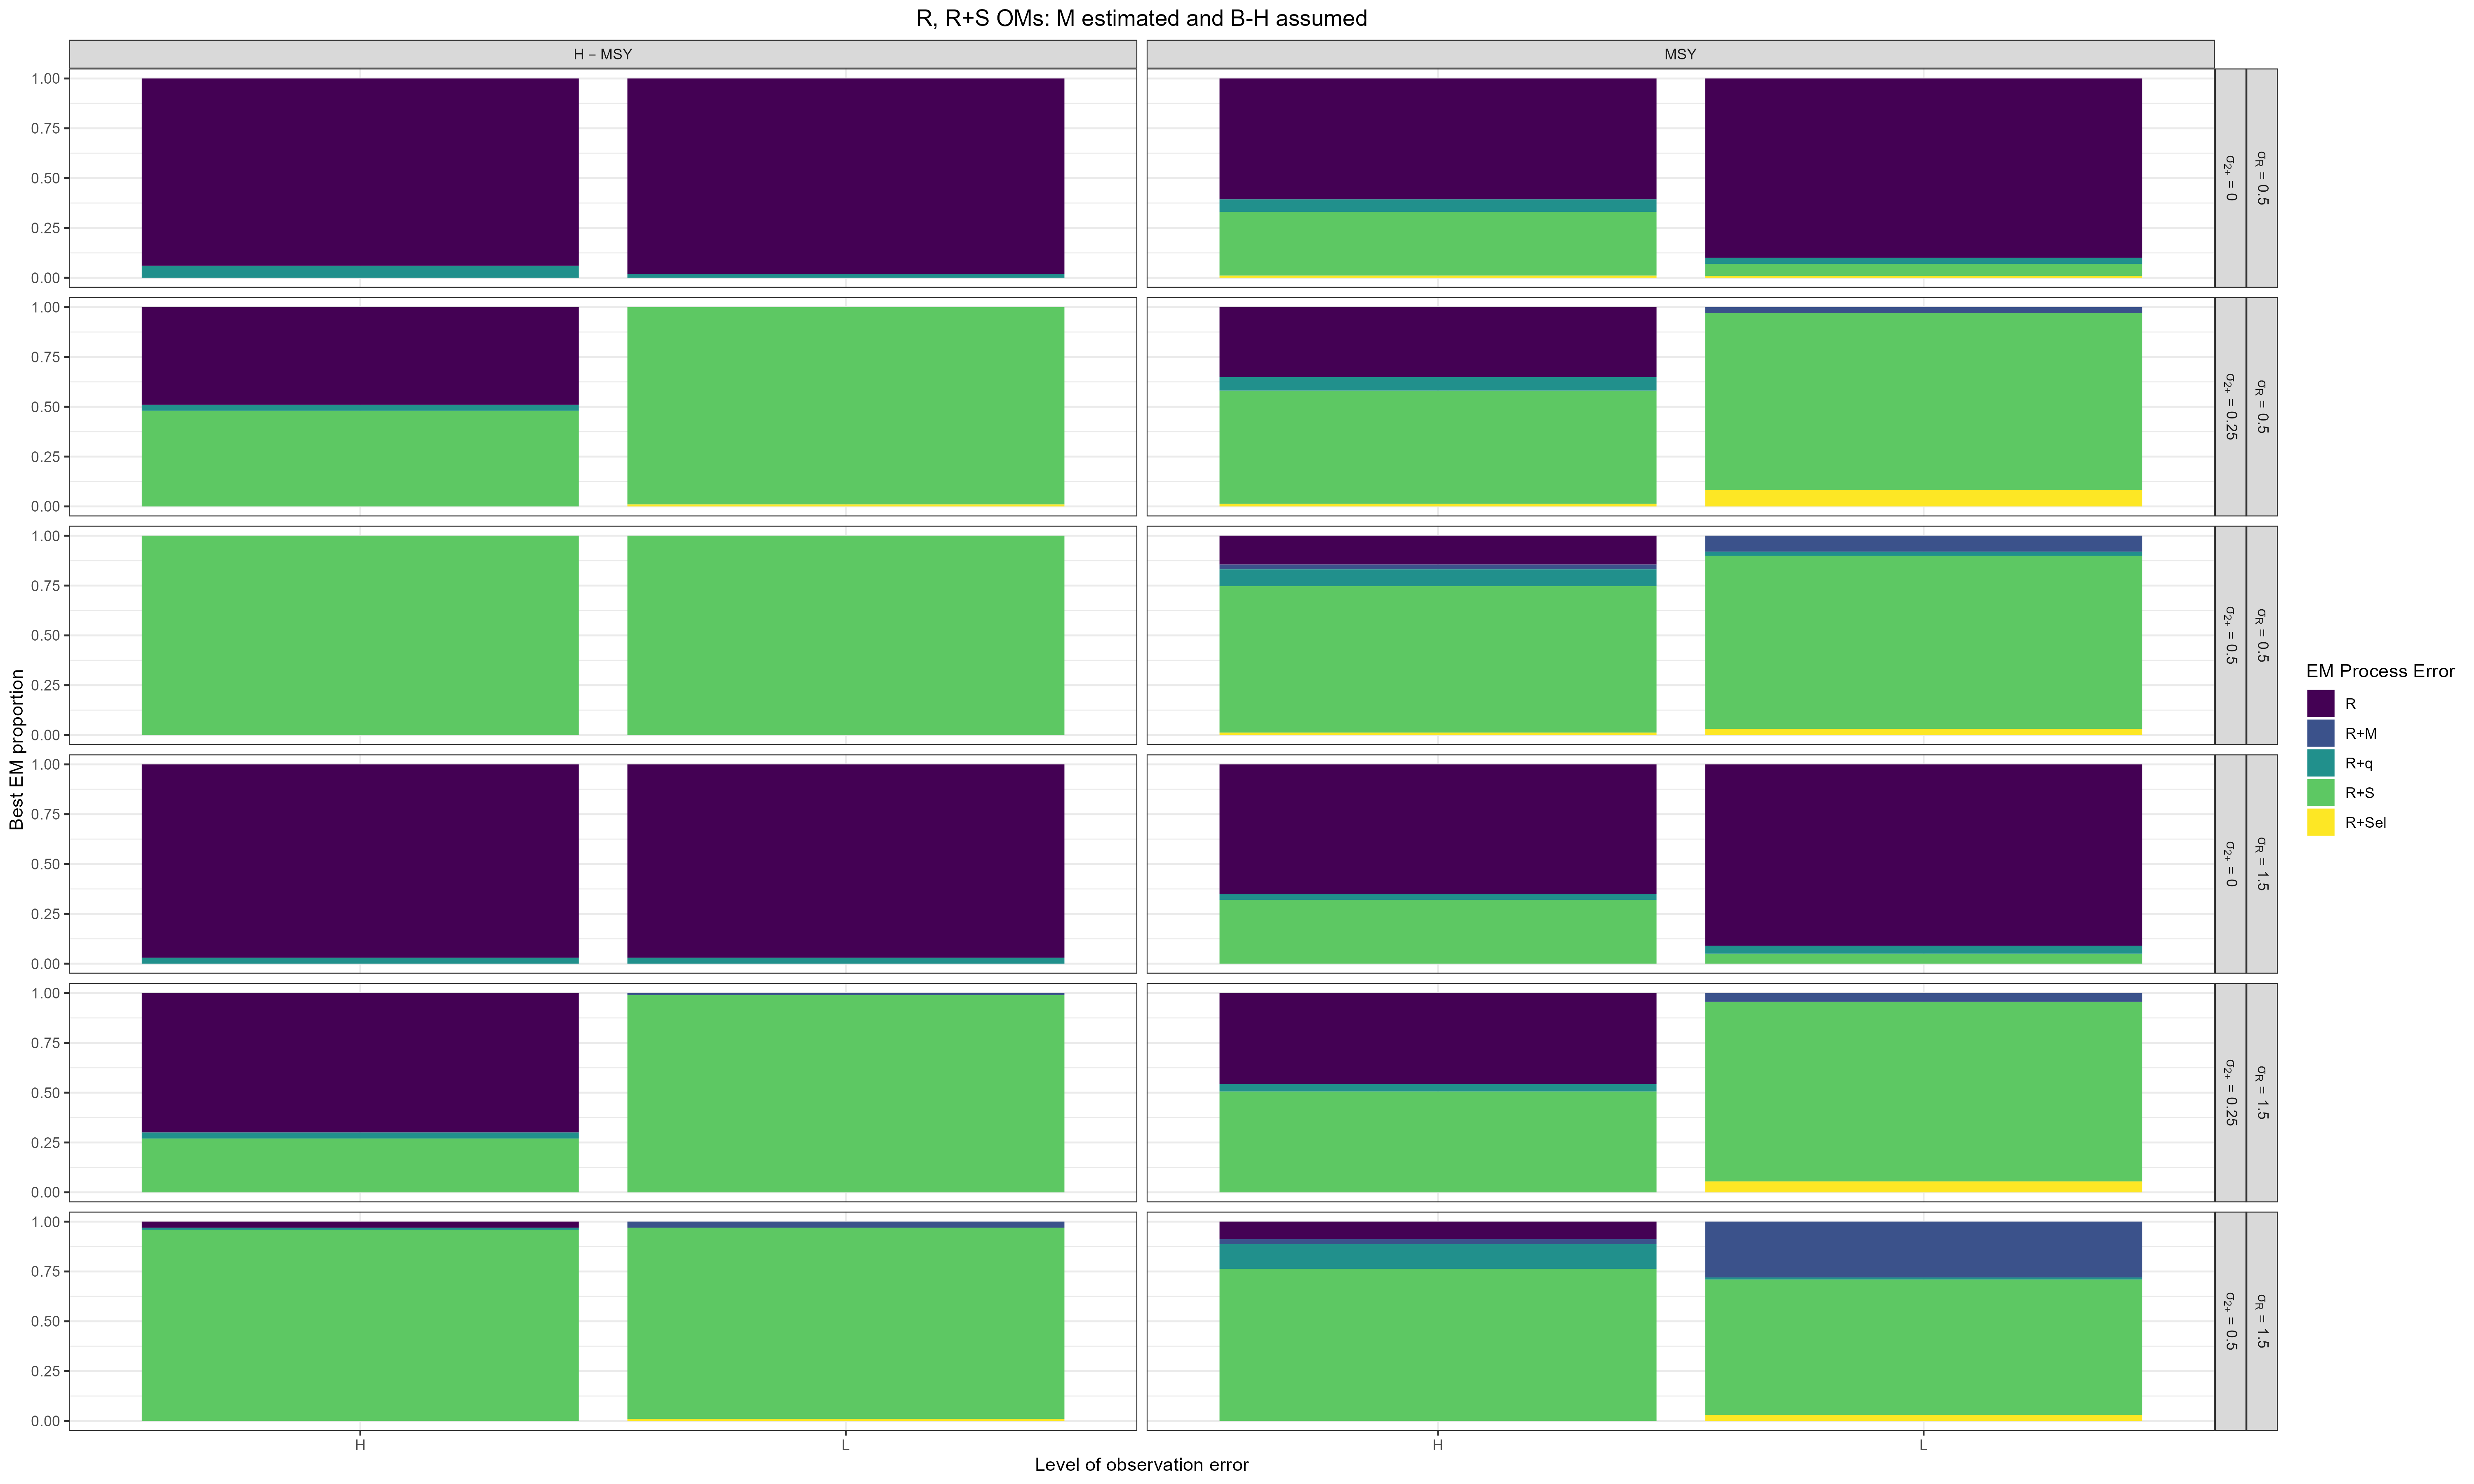
\includegraphics[width = \textwidth]{naa_om_proportion_best_aic_SR_ME.png}
\end{center}
\end{figure}
\end{landscape}

\hypertarget{rm-operating-models-1}{%
\subsubsection*{R+M operating models}\label{rm-operating-models-1}}
\addcontentsline{toc}{subsubsection}{R+M operating models}

Figures \ref{M_om_proportion_best_aic_R_MF} to
\ref{M_om_proportion_best_aic_SR_ME}

\begin{landscape}
\begin{figure}
\caption{Proportion of simulated data sets from OMs with R+M process errors where fitted estimating models had lowest marginal AIC. All estimating models estimate mean recruitment rather than a stock-recruit relationship and and M is fixed at the true value.} \label{M_om_proportion_best_aic_R_MF}
\begin{center}
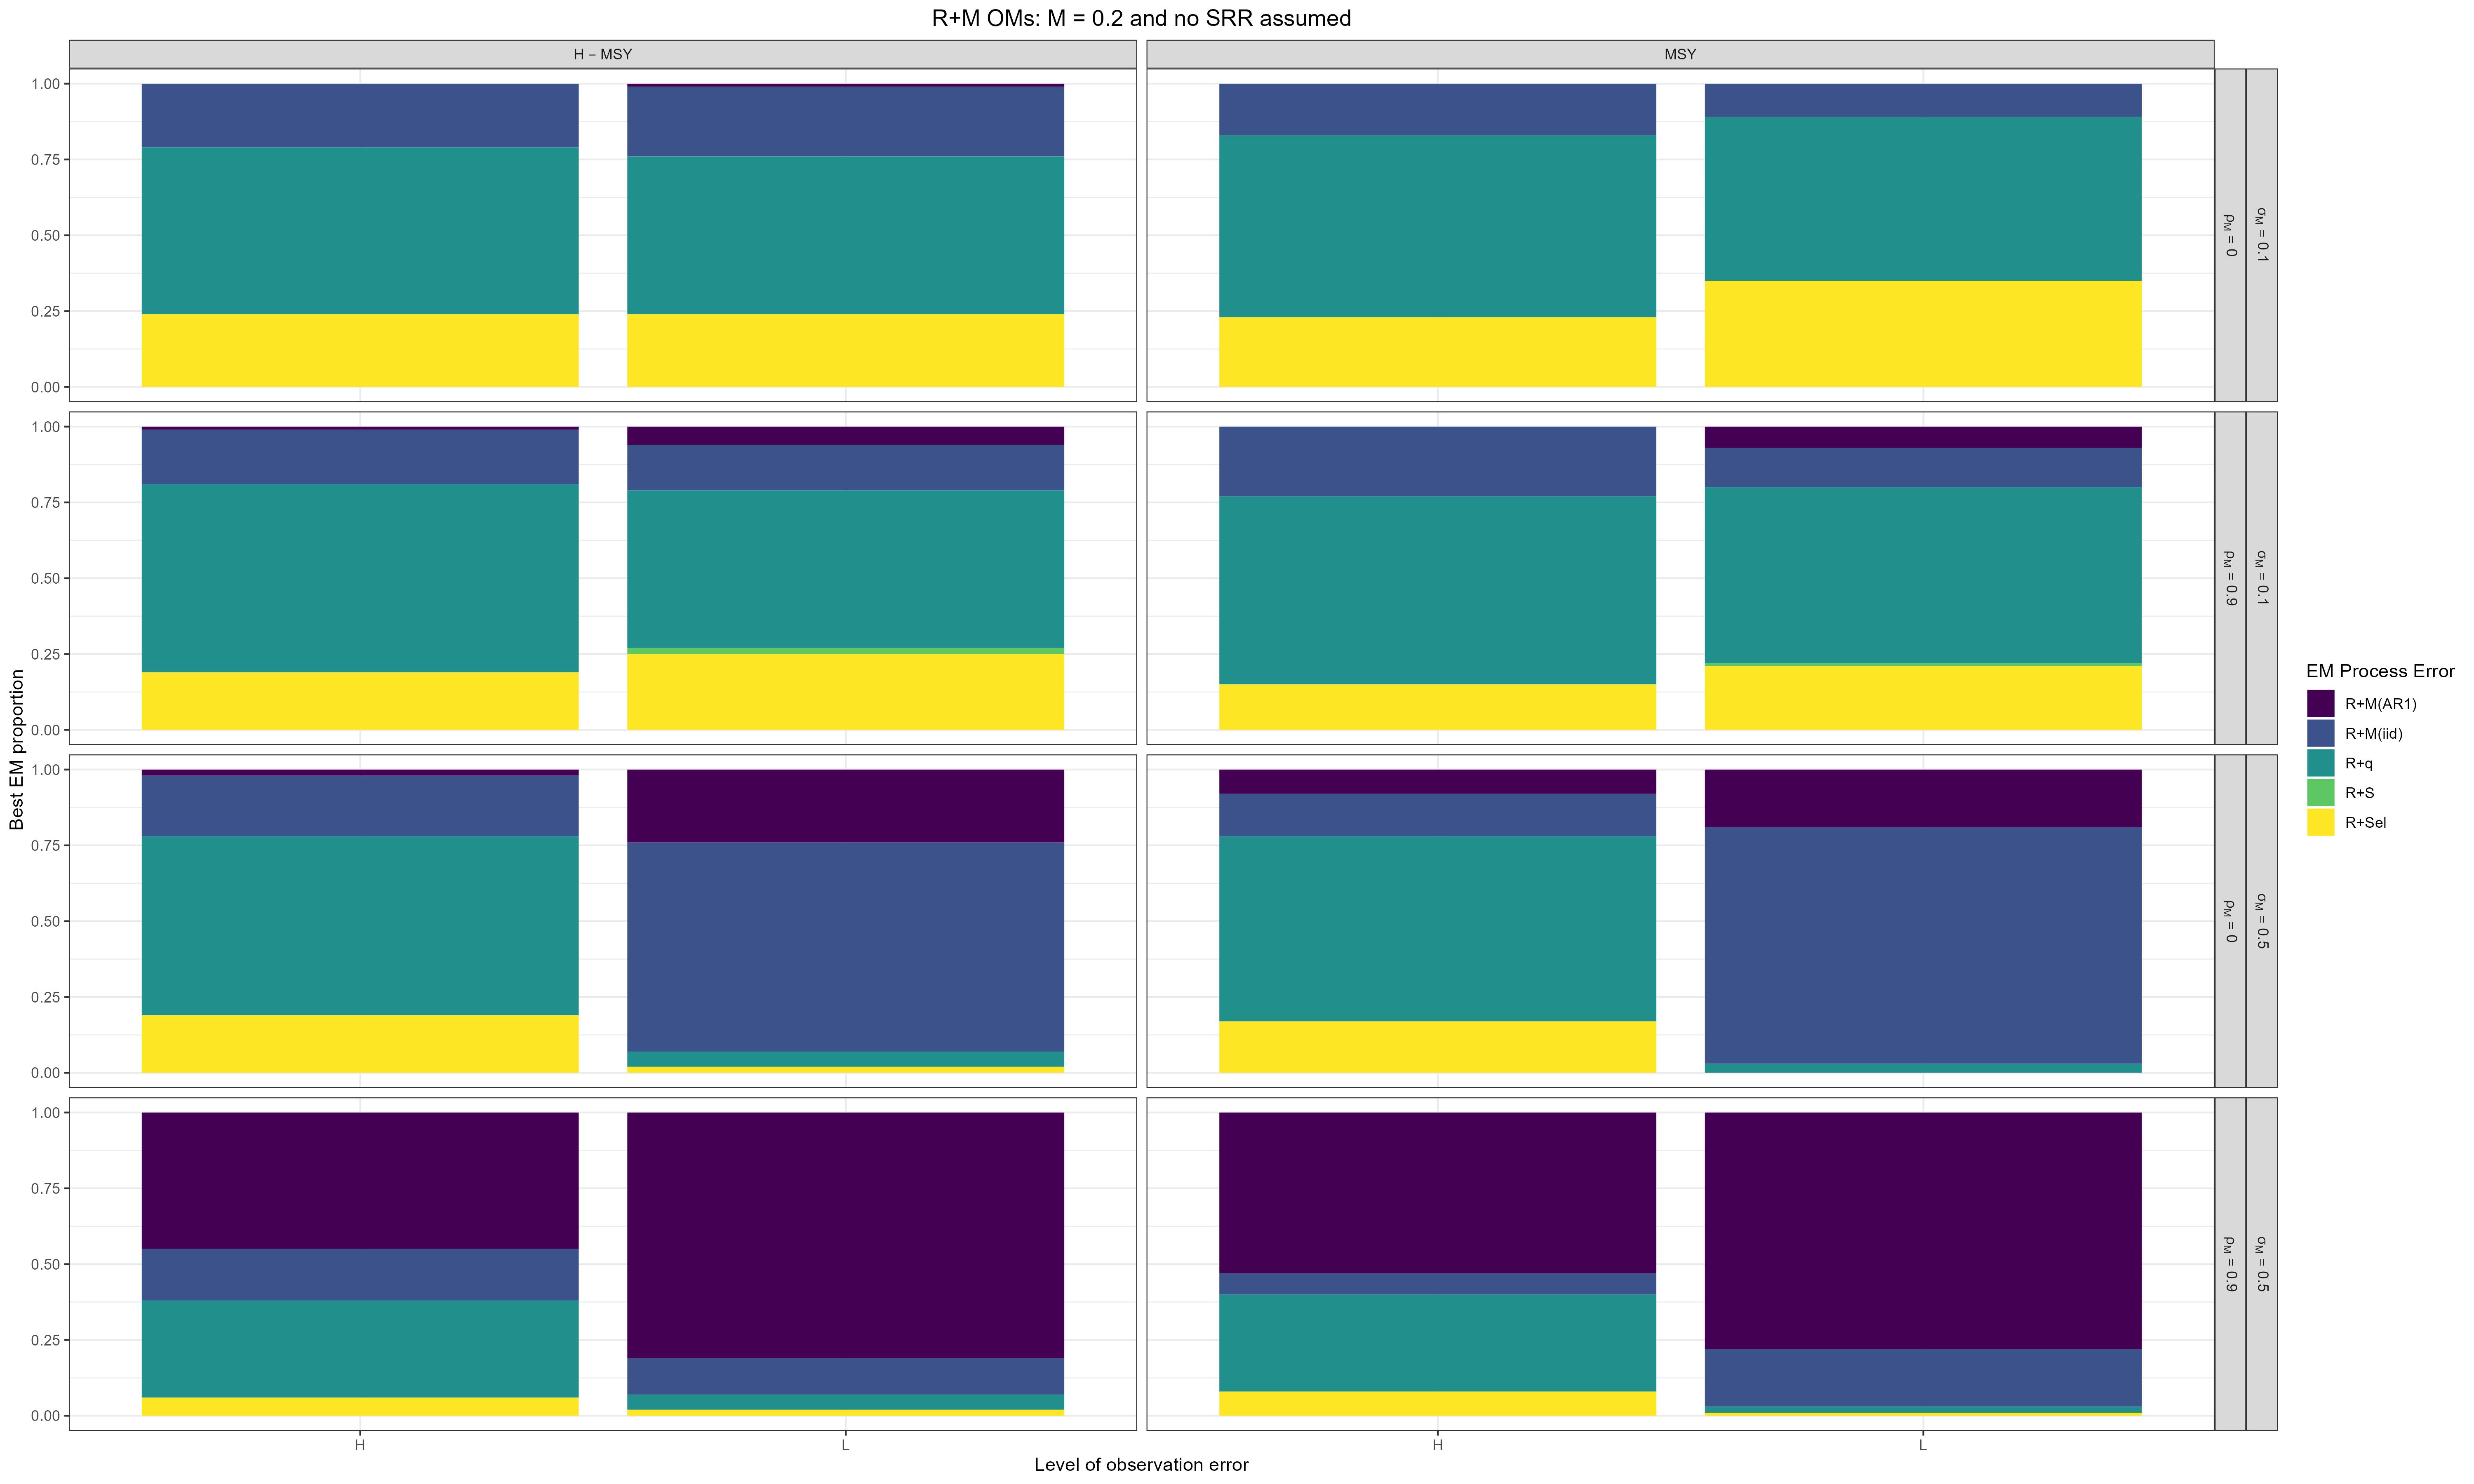
\includegraphics[width = \textwidth]{M_om_proportion_best_aic_R_MF.png}
\end{center}
\end{figure}
\end{landscape}

\begin{landscape}
\begin{figure}
\caption{Proportion of simulated data sets from OMs with R+M process errors where fitted estimating models had lowest marginal AIC. All estimating models estimate mean recruitment rather than a stock-recruit relationship and and M is estimated.} \label{M_om_proportion_best_aic_R_ME}
\begin{center}
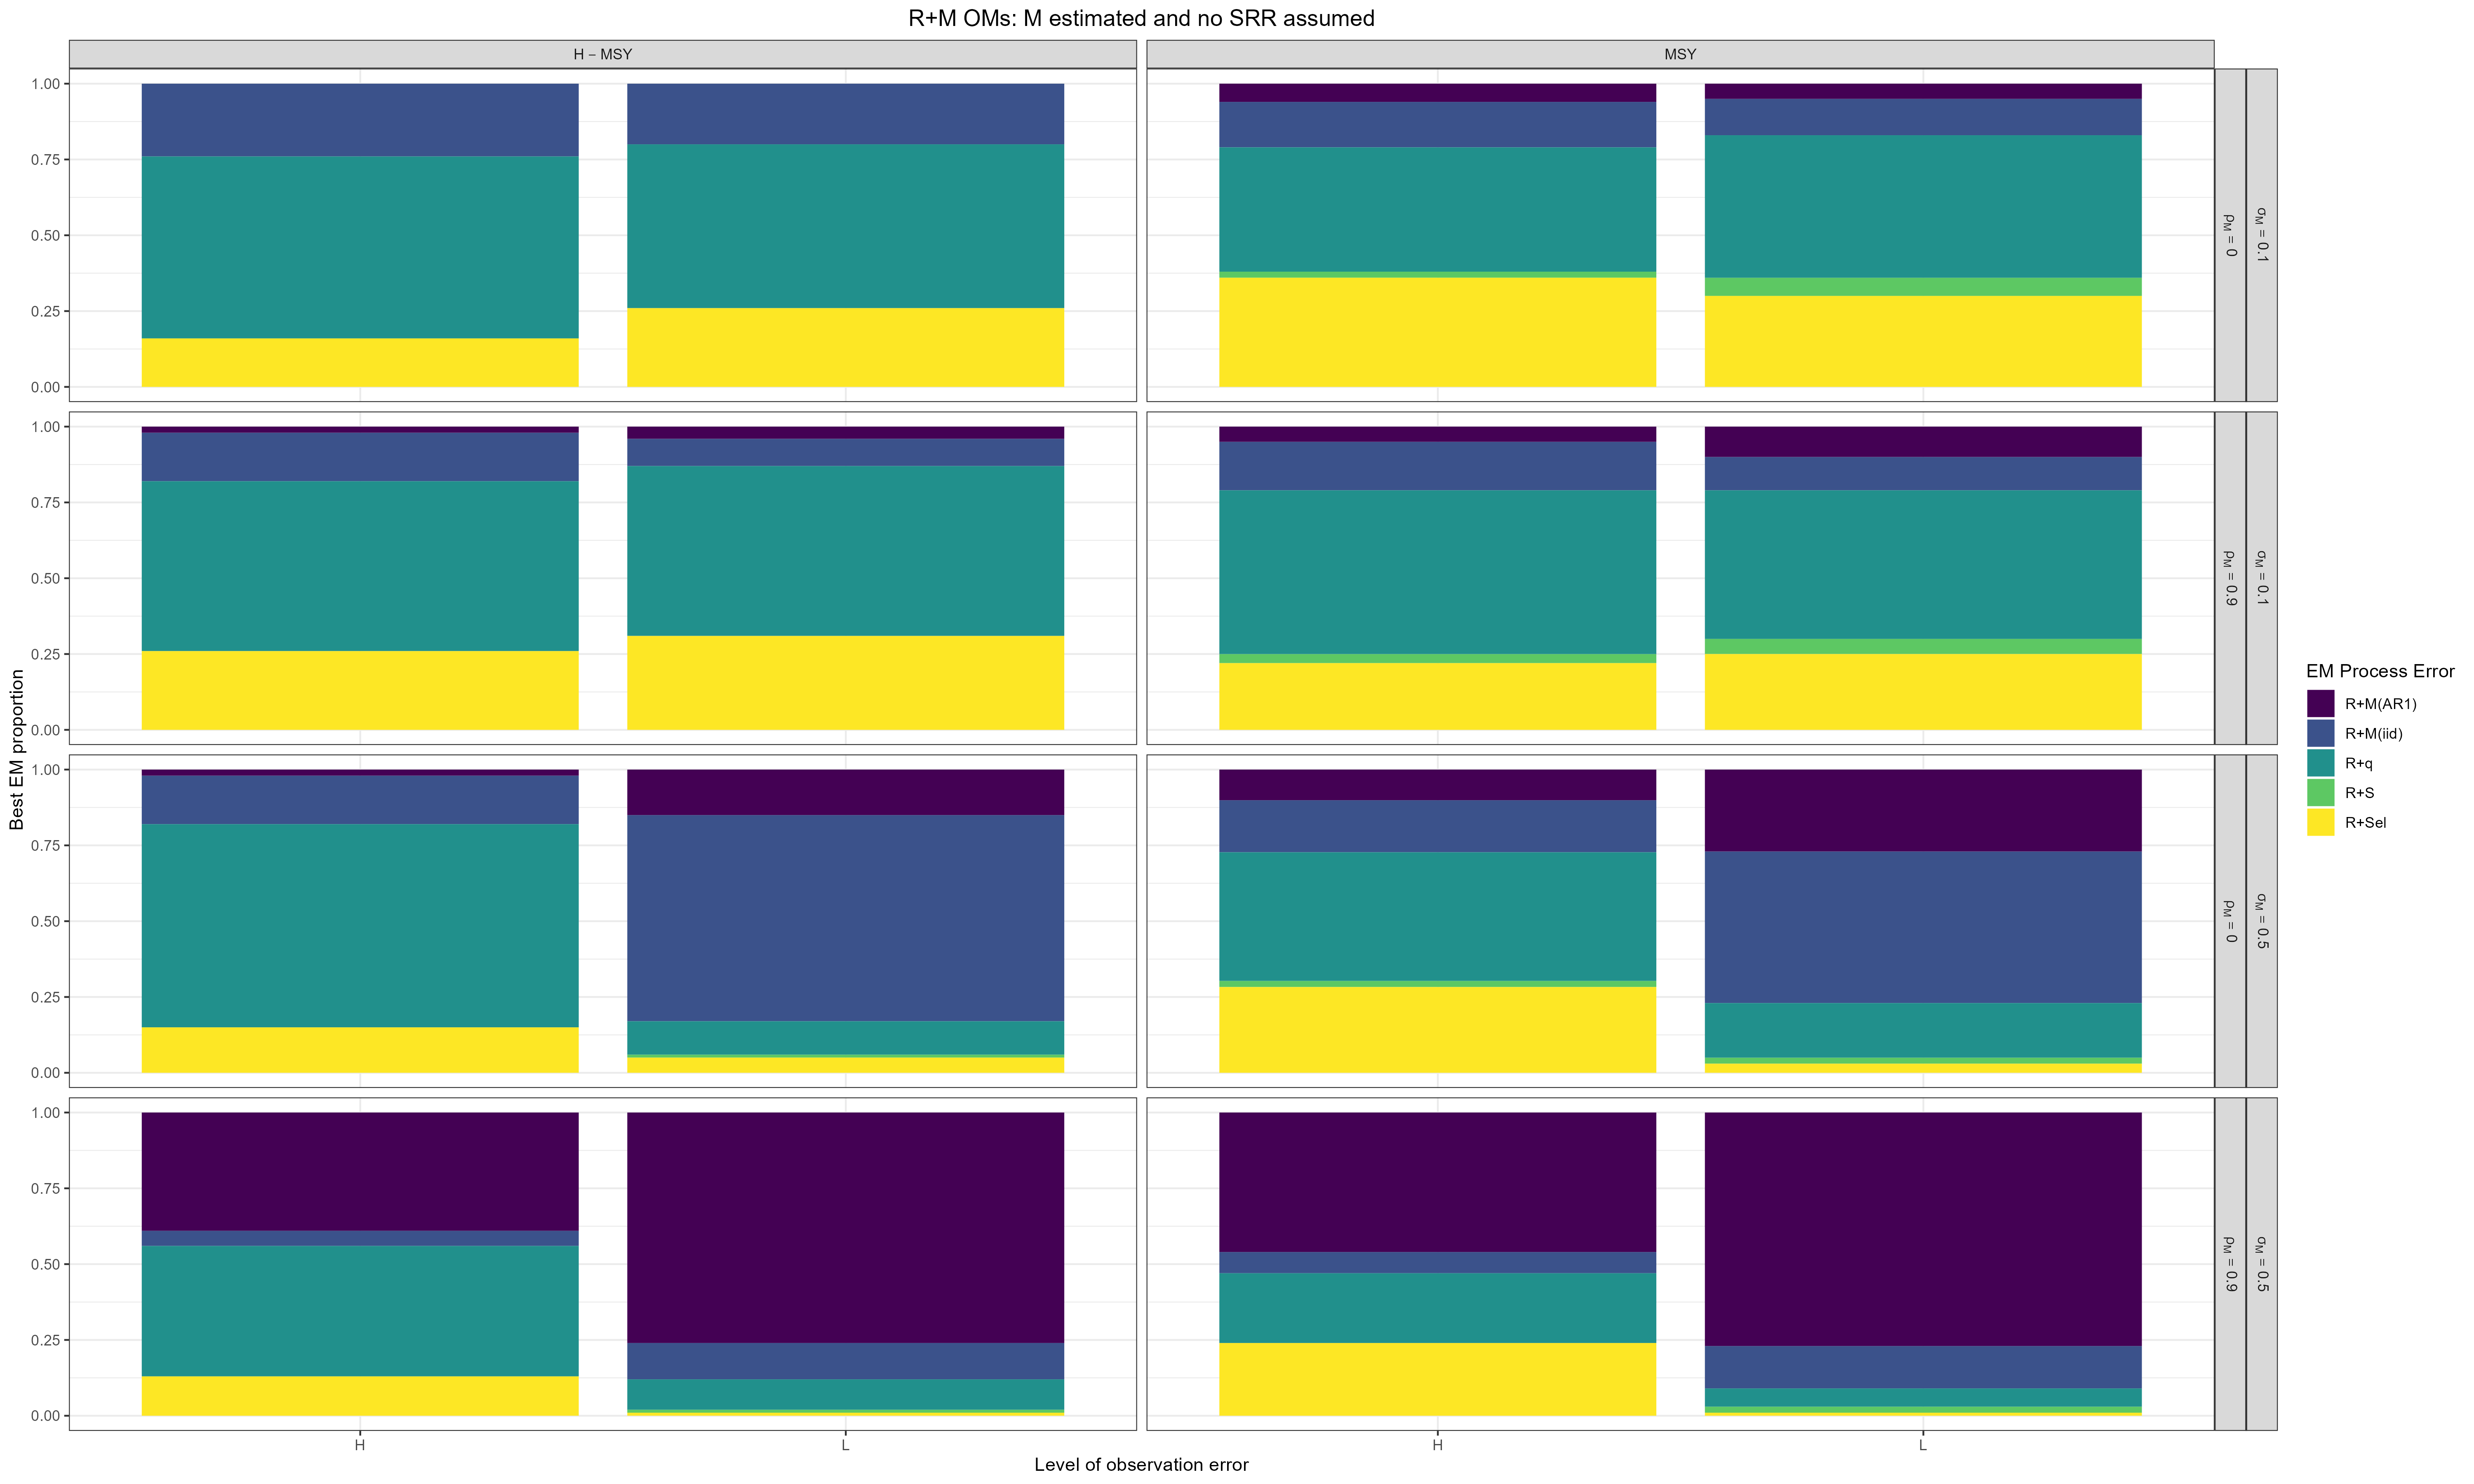
\includegraphics[width = \textwidth]{M_om_proportion_best_aic_R_ME.png}
\end{center}
\end{figure}
\end{landscape}

\begin{landscape}
\begin{figure}
\caption{Proportion of simulated data sets from OMs with R+M process errors where fitted estimating models had lowest marginal AIC. All estimating models estimate a stock-recruit relationship and and M is fixed at the true value.} \label{M_om_proportion_best_aic_SR_MF}
\begin{center}
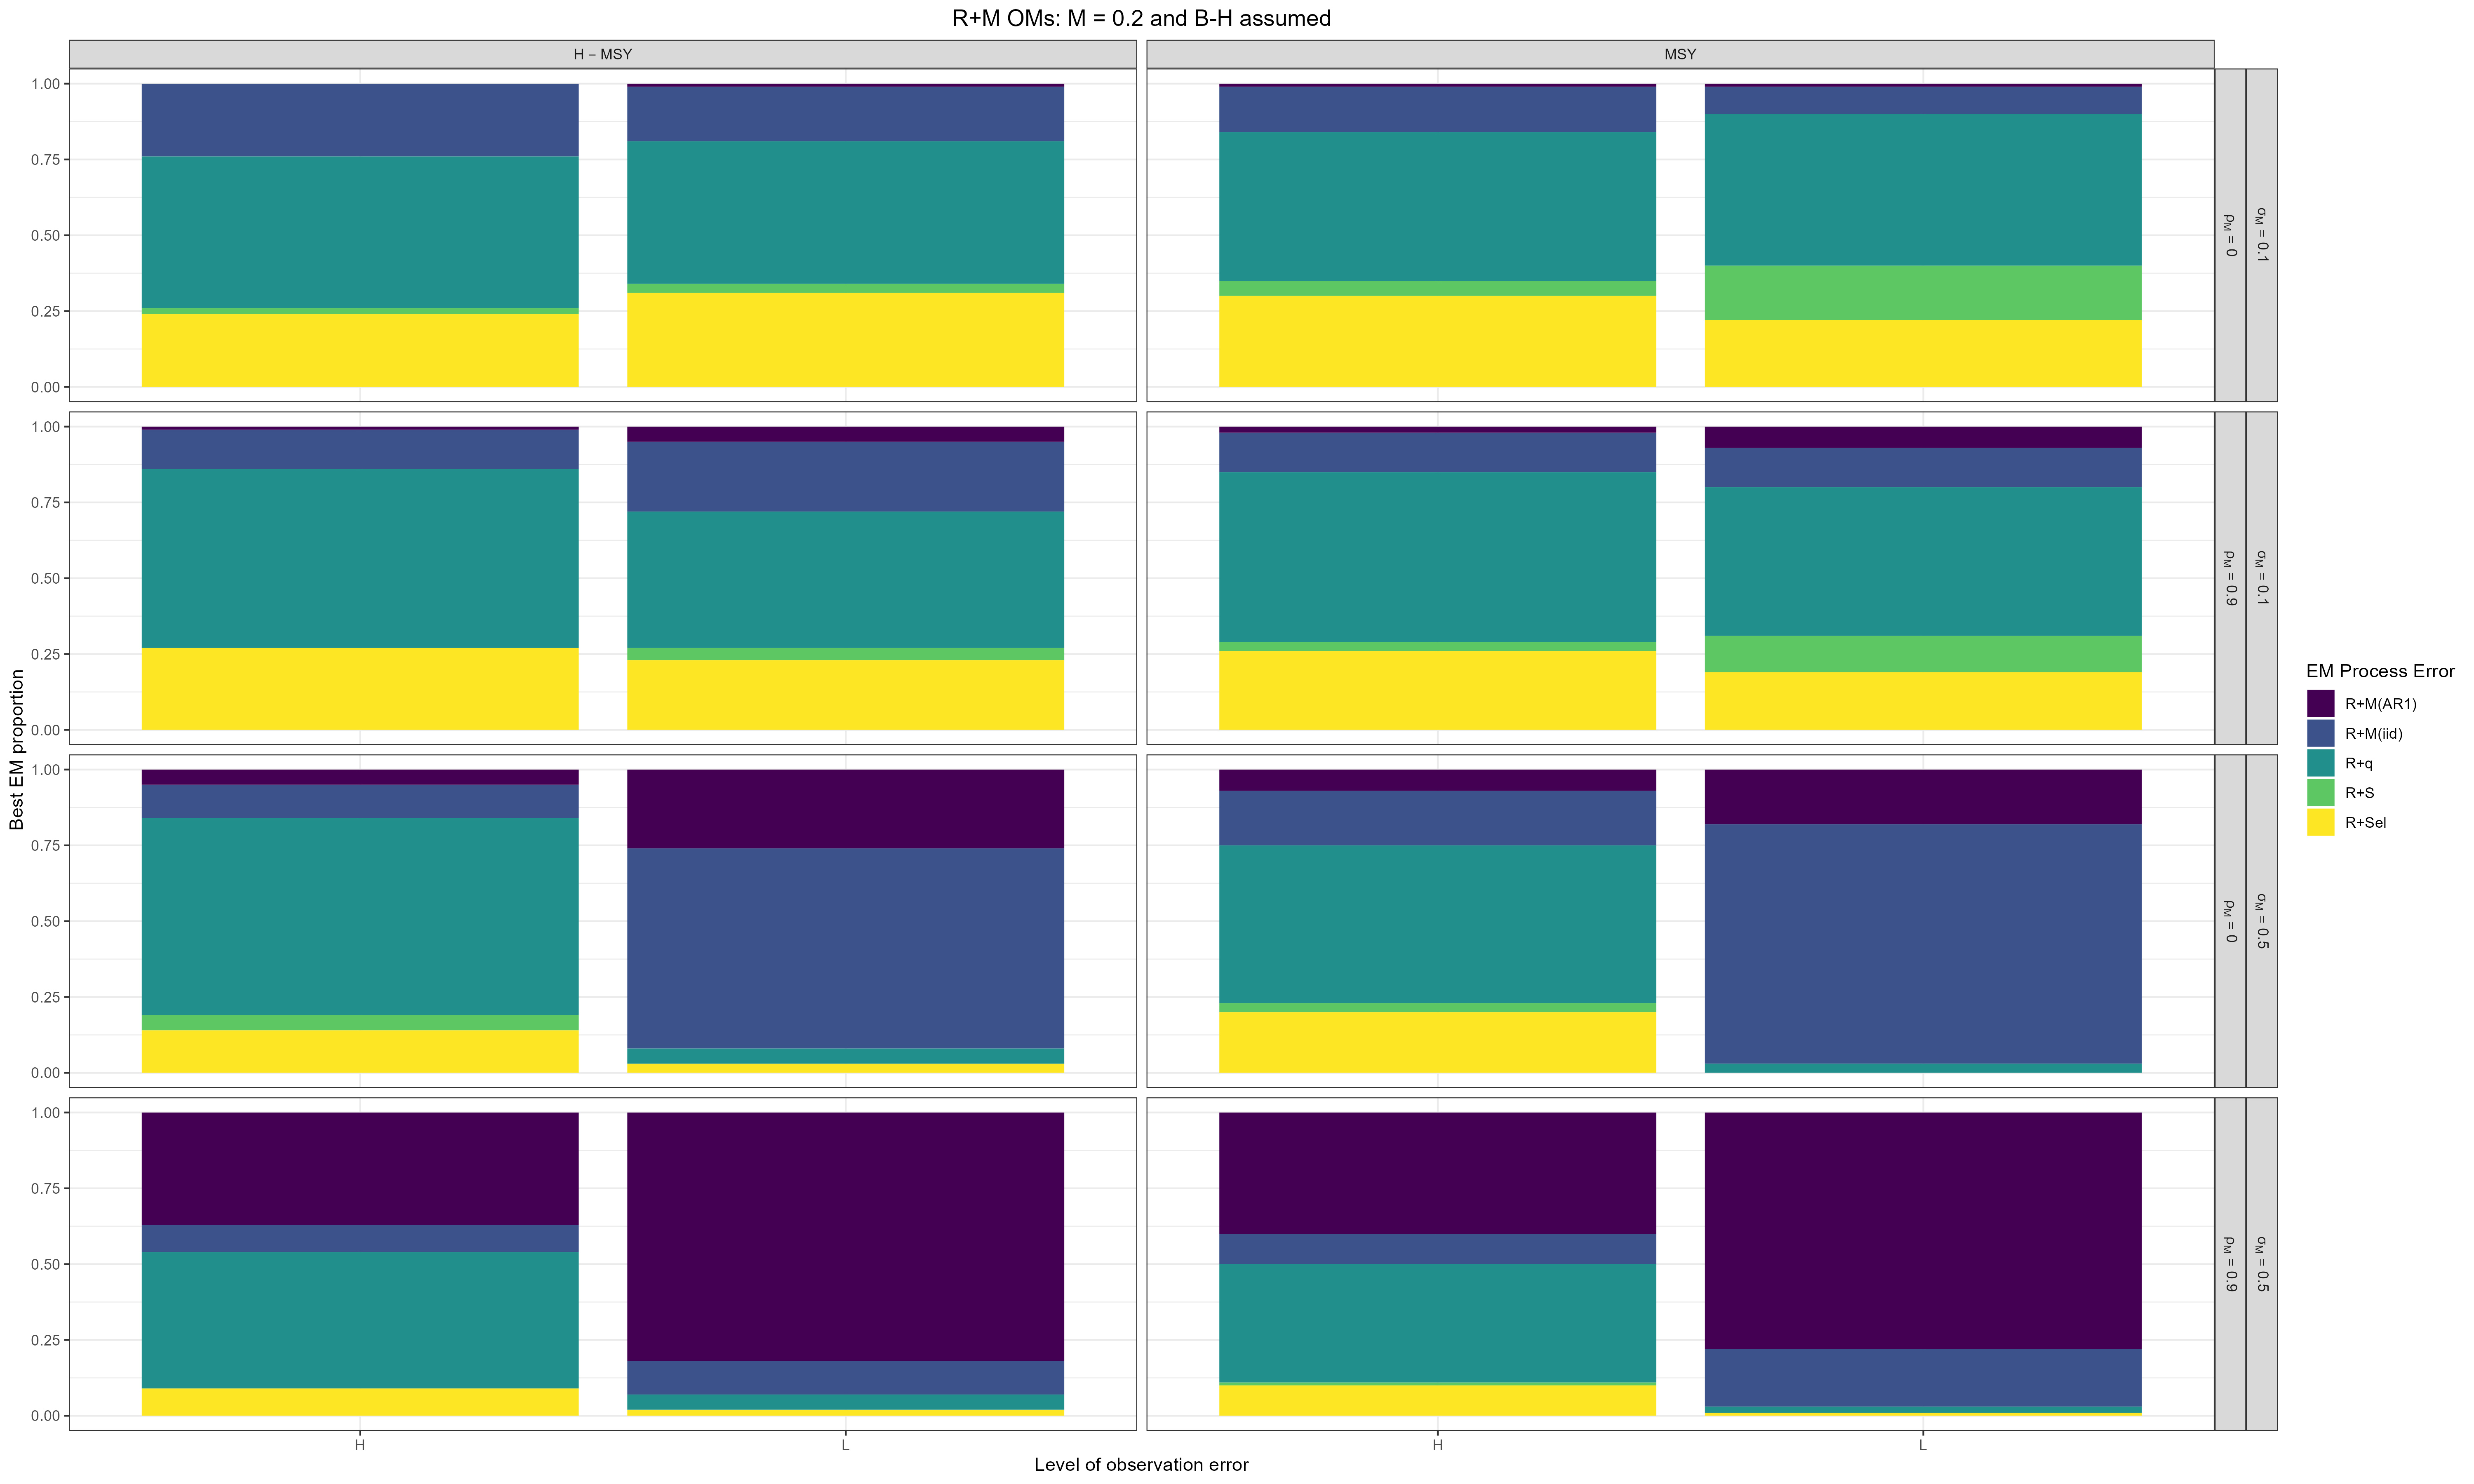
\includegraphics[width = \textwidth]{M_om_proportion_best_aic_SR_MF.png}
\end{center}
\end{figure}
\end{landscape}

\begin{landscape}
\begin{figure}
\caption{Proportion of simulated data sets from OMs with R+M process errors where fitted estimating models had lowest marginal AIC. All estimating models estimate a stock-recruit relationship and and M is estimated.} \label{M_om_proportion_best_aic_SR_ME}
\begin{center}
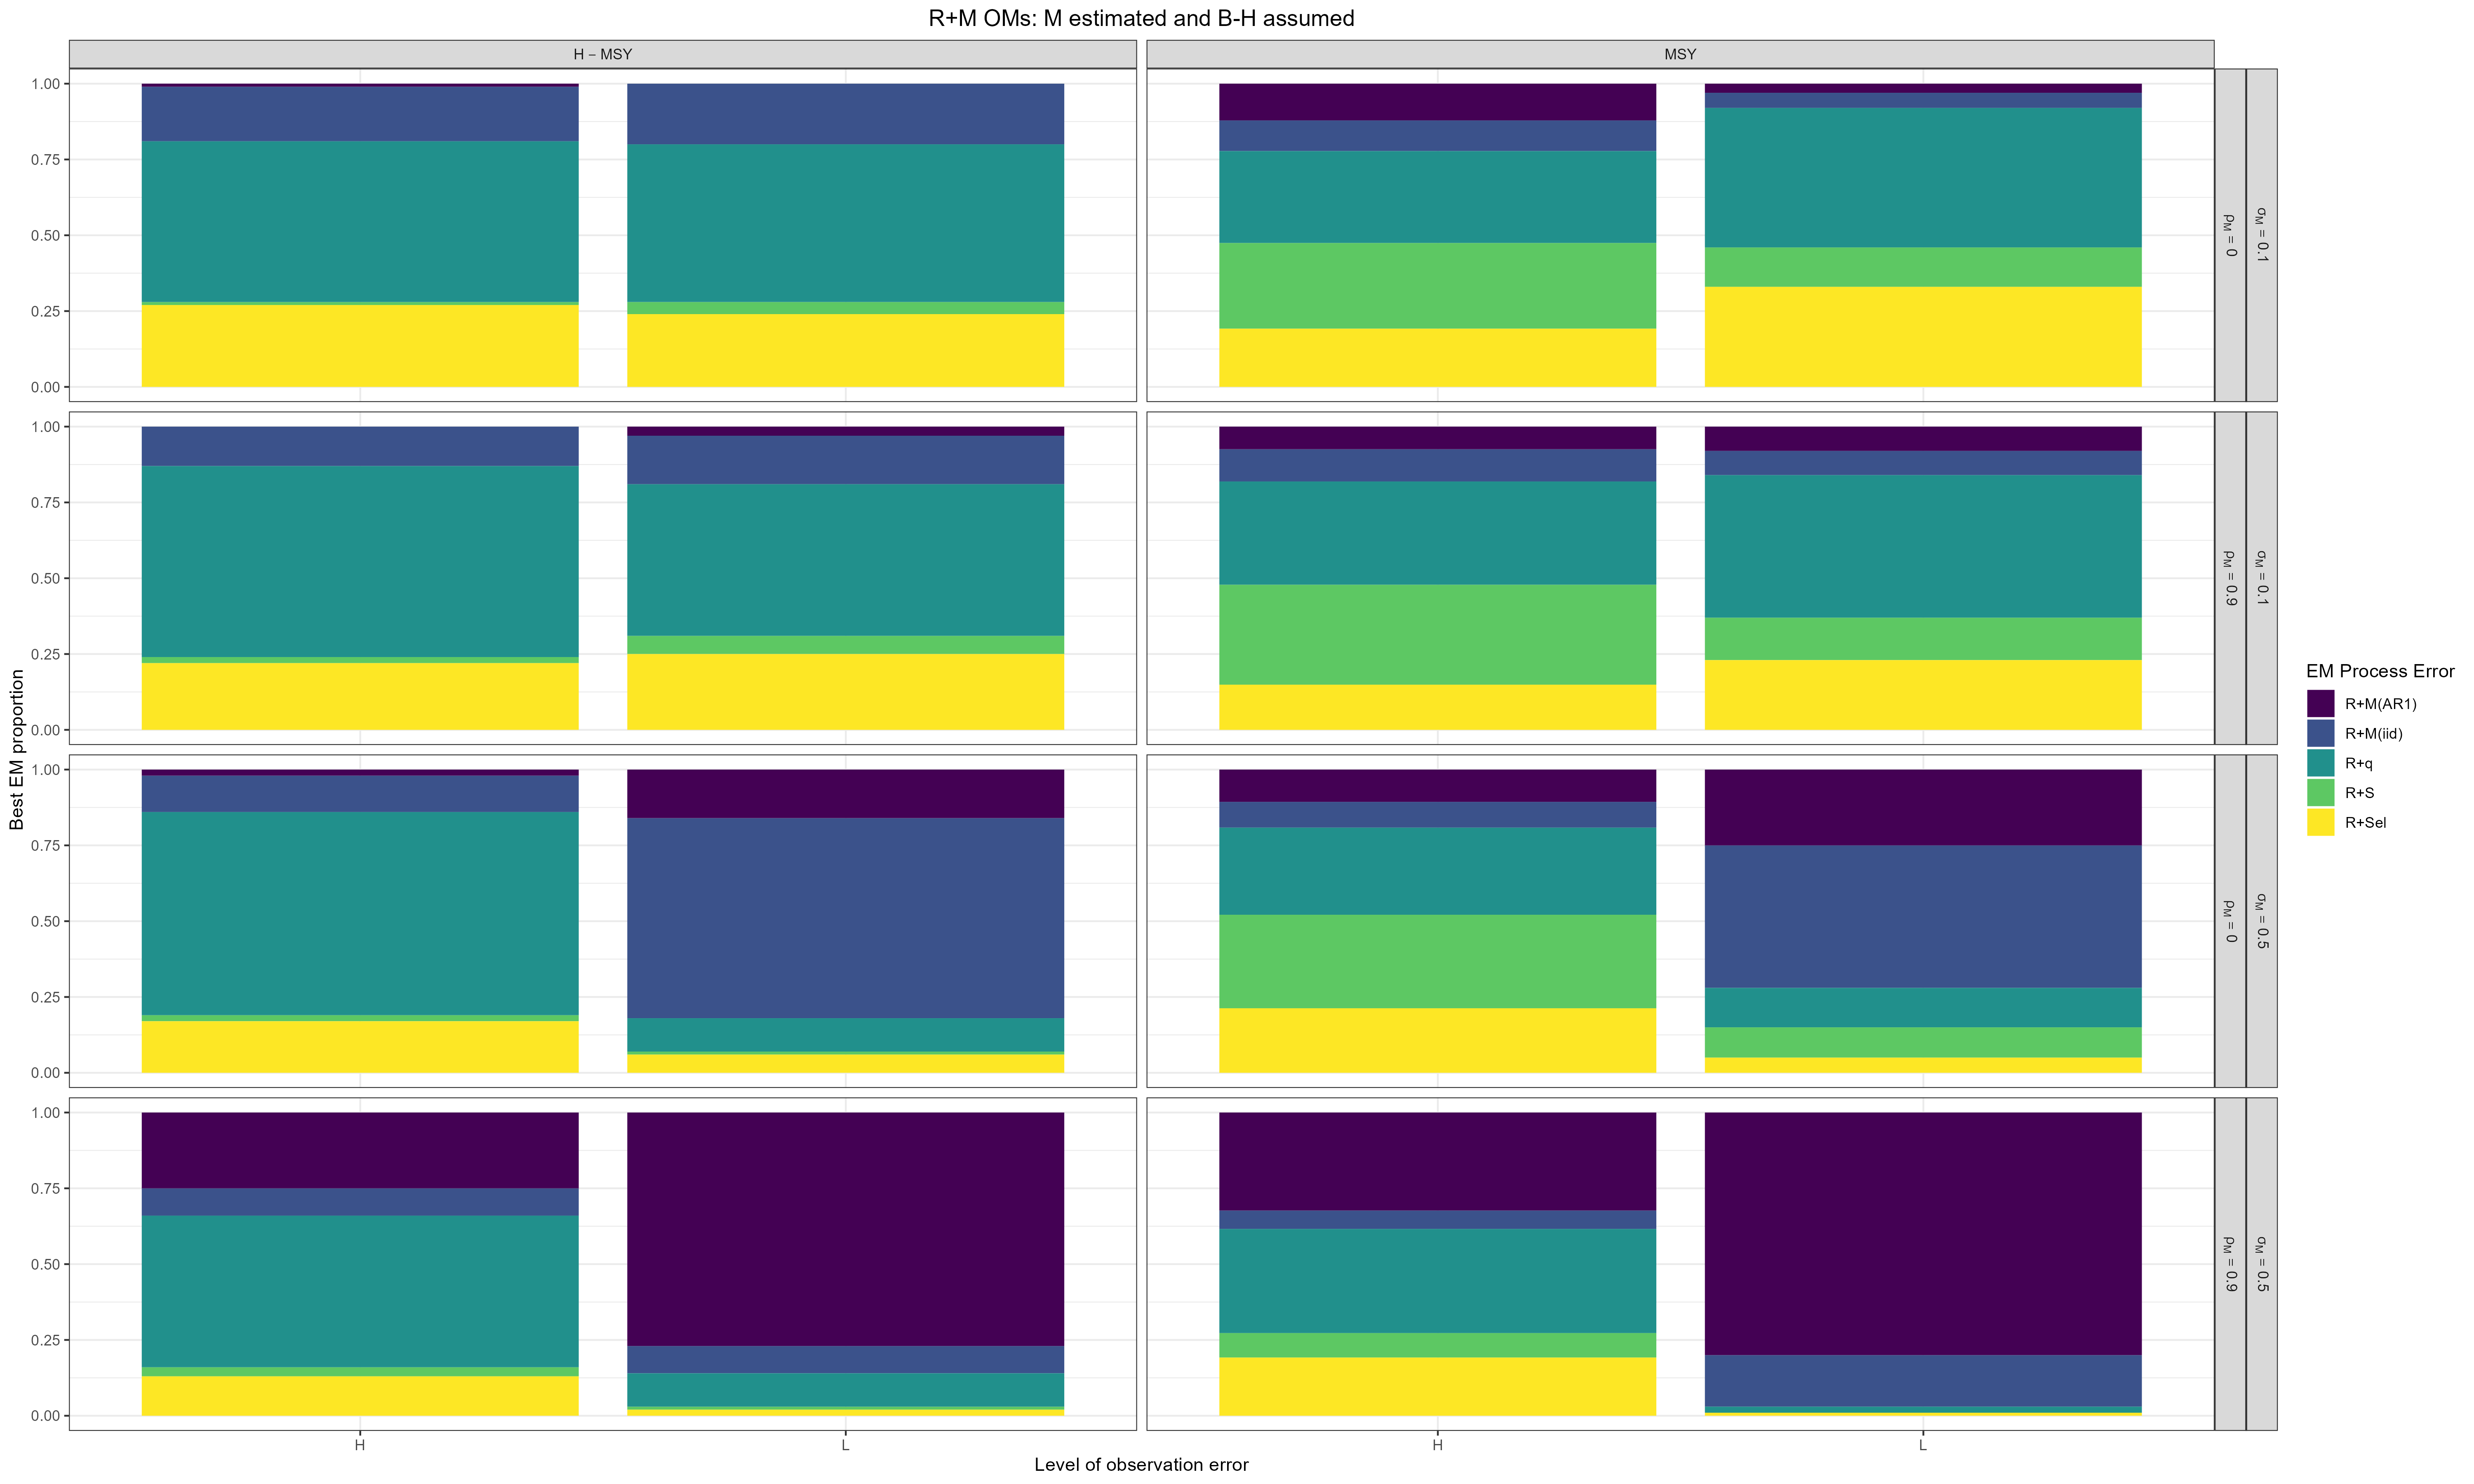
\includegraphics[width = \textwidth]{M_om_proportion_best_aic_SR_ME.png}
\end{center}
\end{figure}
\end{landscape}

\hypertarget{rsel-operating-models-1}{%
\subsubsection*{R+Sel operating models}\label{rsel-operating-models-1}}
\addcontentsline{toc}{subsubsection}{R+Sel operating models}

Figures \ref{Sel_om_proportion_best_aic_R_MF} to
\ref{Sel_om_proportion_best_aic_SR_ME}

\begin{landscape}
\begin{figure}
\caption{Proportion of simulated data sets from OMs with R+Sel process errors where fitted estimating models had lowest marginal AIC. All estimating models estimate mean recruitment rather than a stock-recruit relationship and and M is fixed at the true value.} \label{Sel_om_proportion_best_aic_R_MF}
\begin{center}
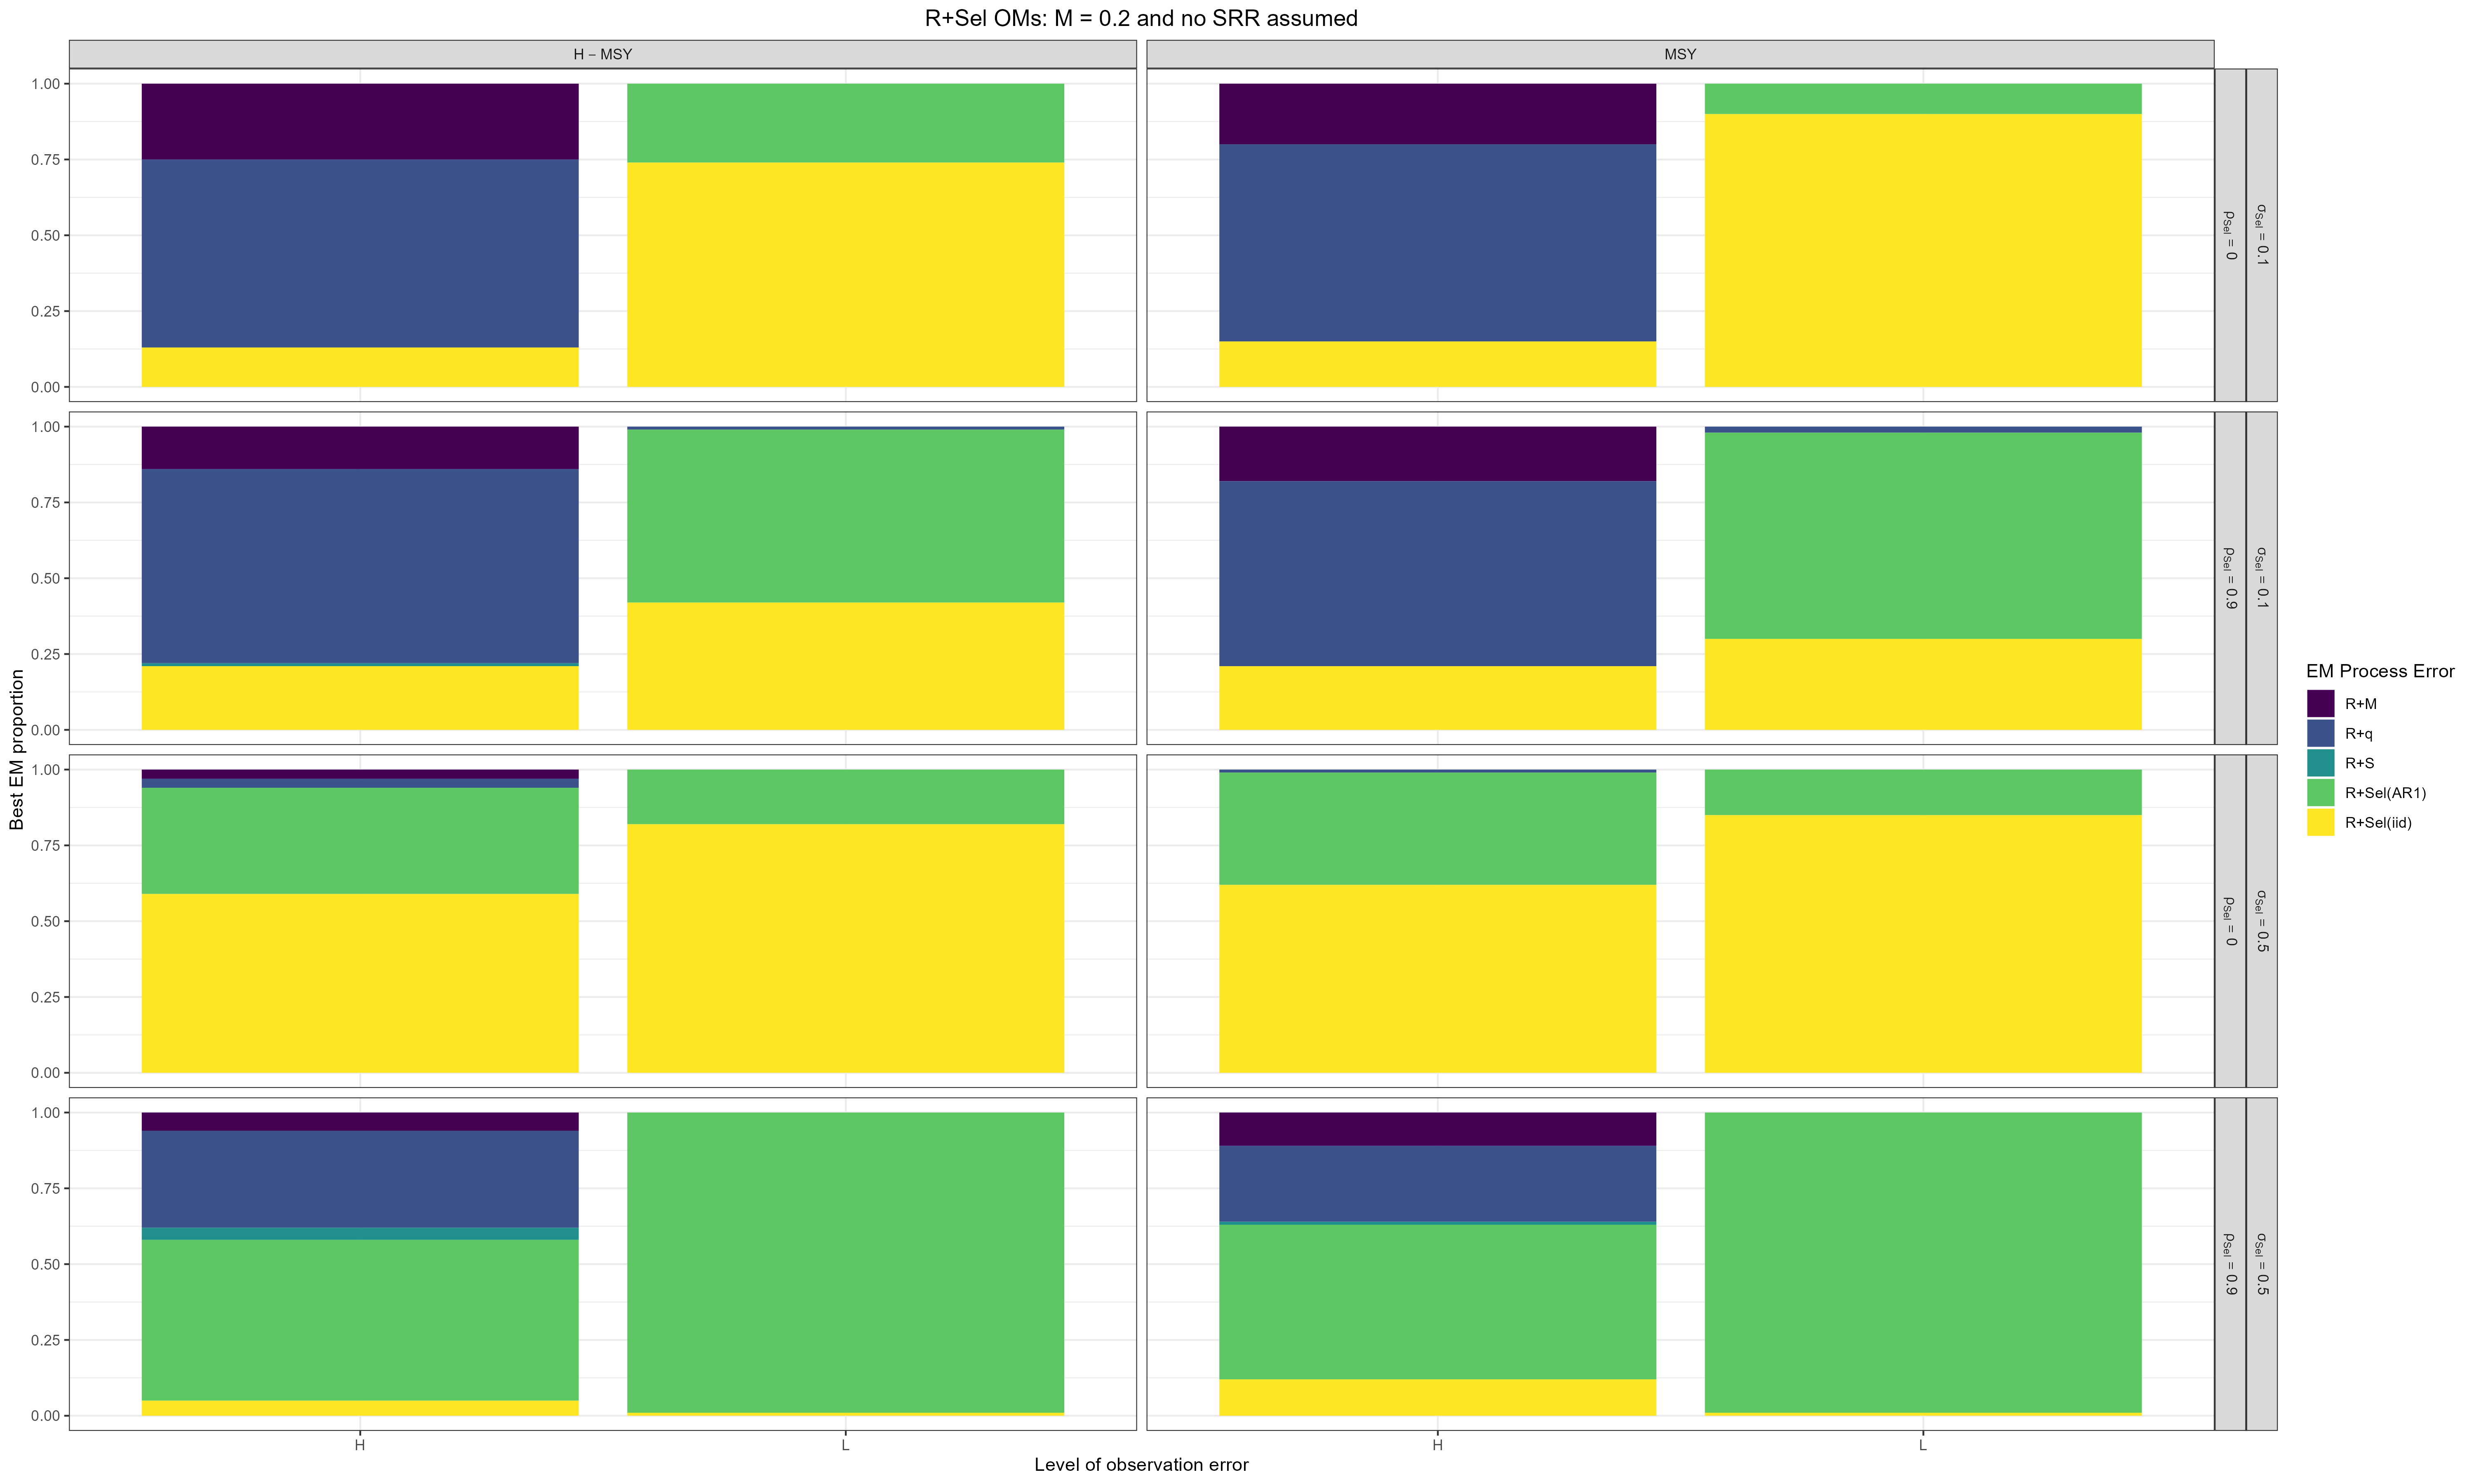
\includegraphics[width = \textwidth]{Sel_om_proportion_best_aic_R_MF.png}
\end{center}
\end{figure}
\end{landscape}

\begin{landscape}
\begin{figure}
\caption{Proportion of simulated data sets from OMs with R+Sel process errors where fitted estimating models had lowest marginal AIC. All estimating models estimate mean recruitment rather than a stock-recruit relationship and and M is estimated.} \label{Sel_om_proportion_best_aic_R_ME}
\begin{center}
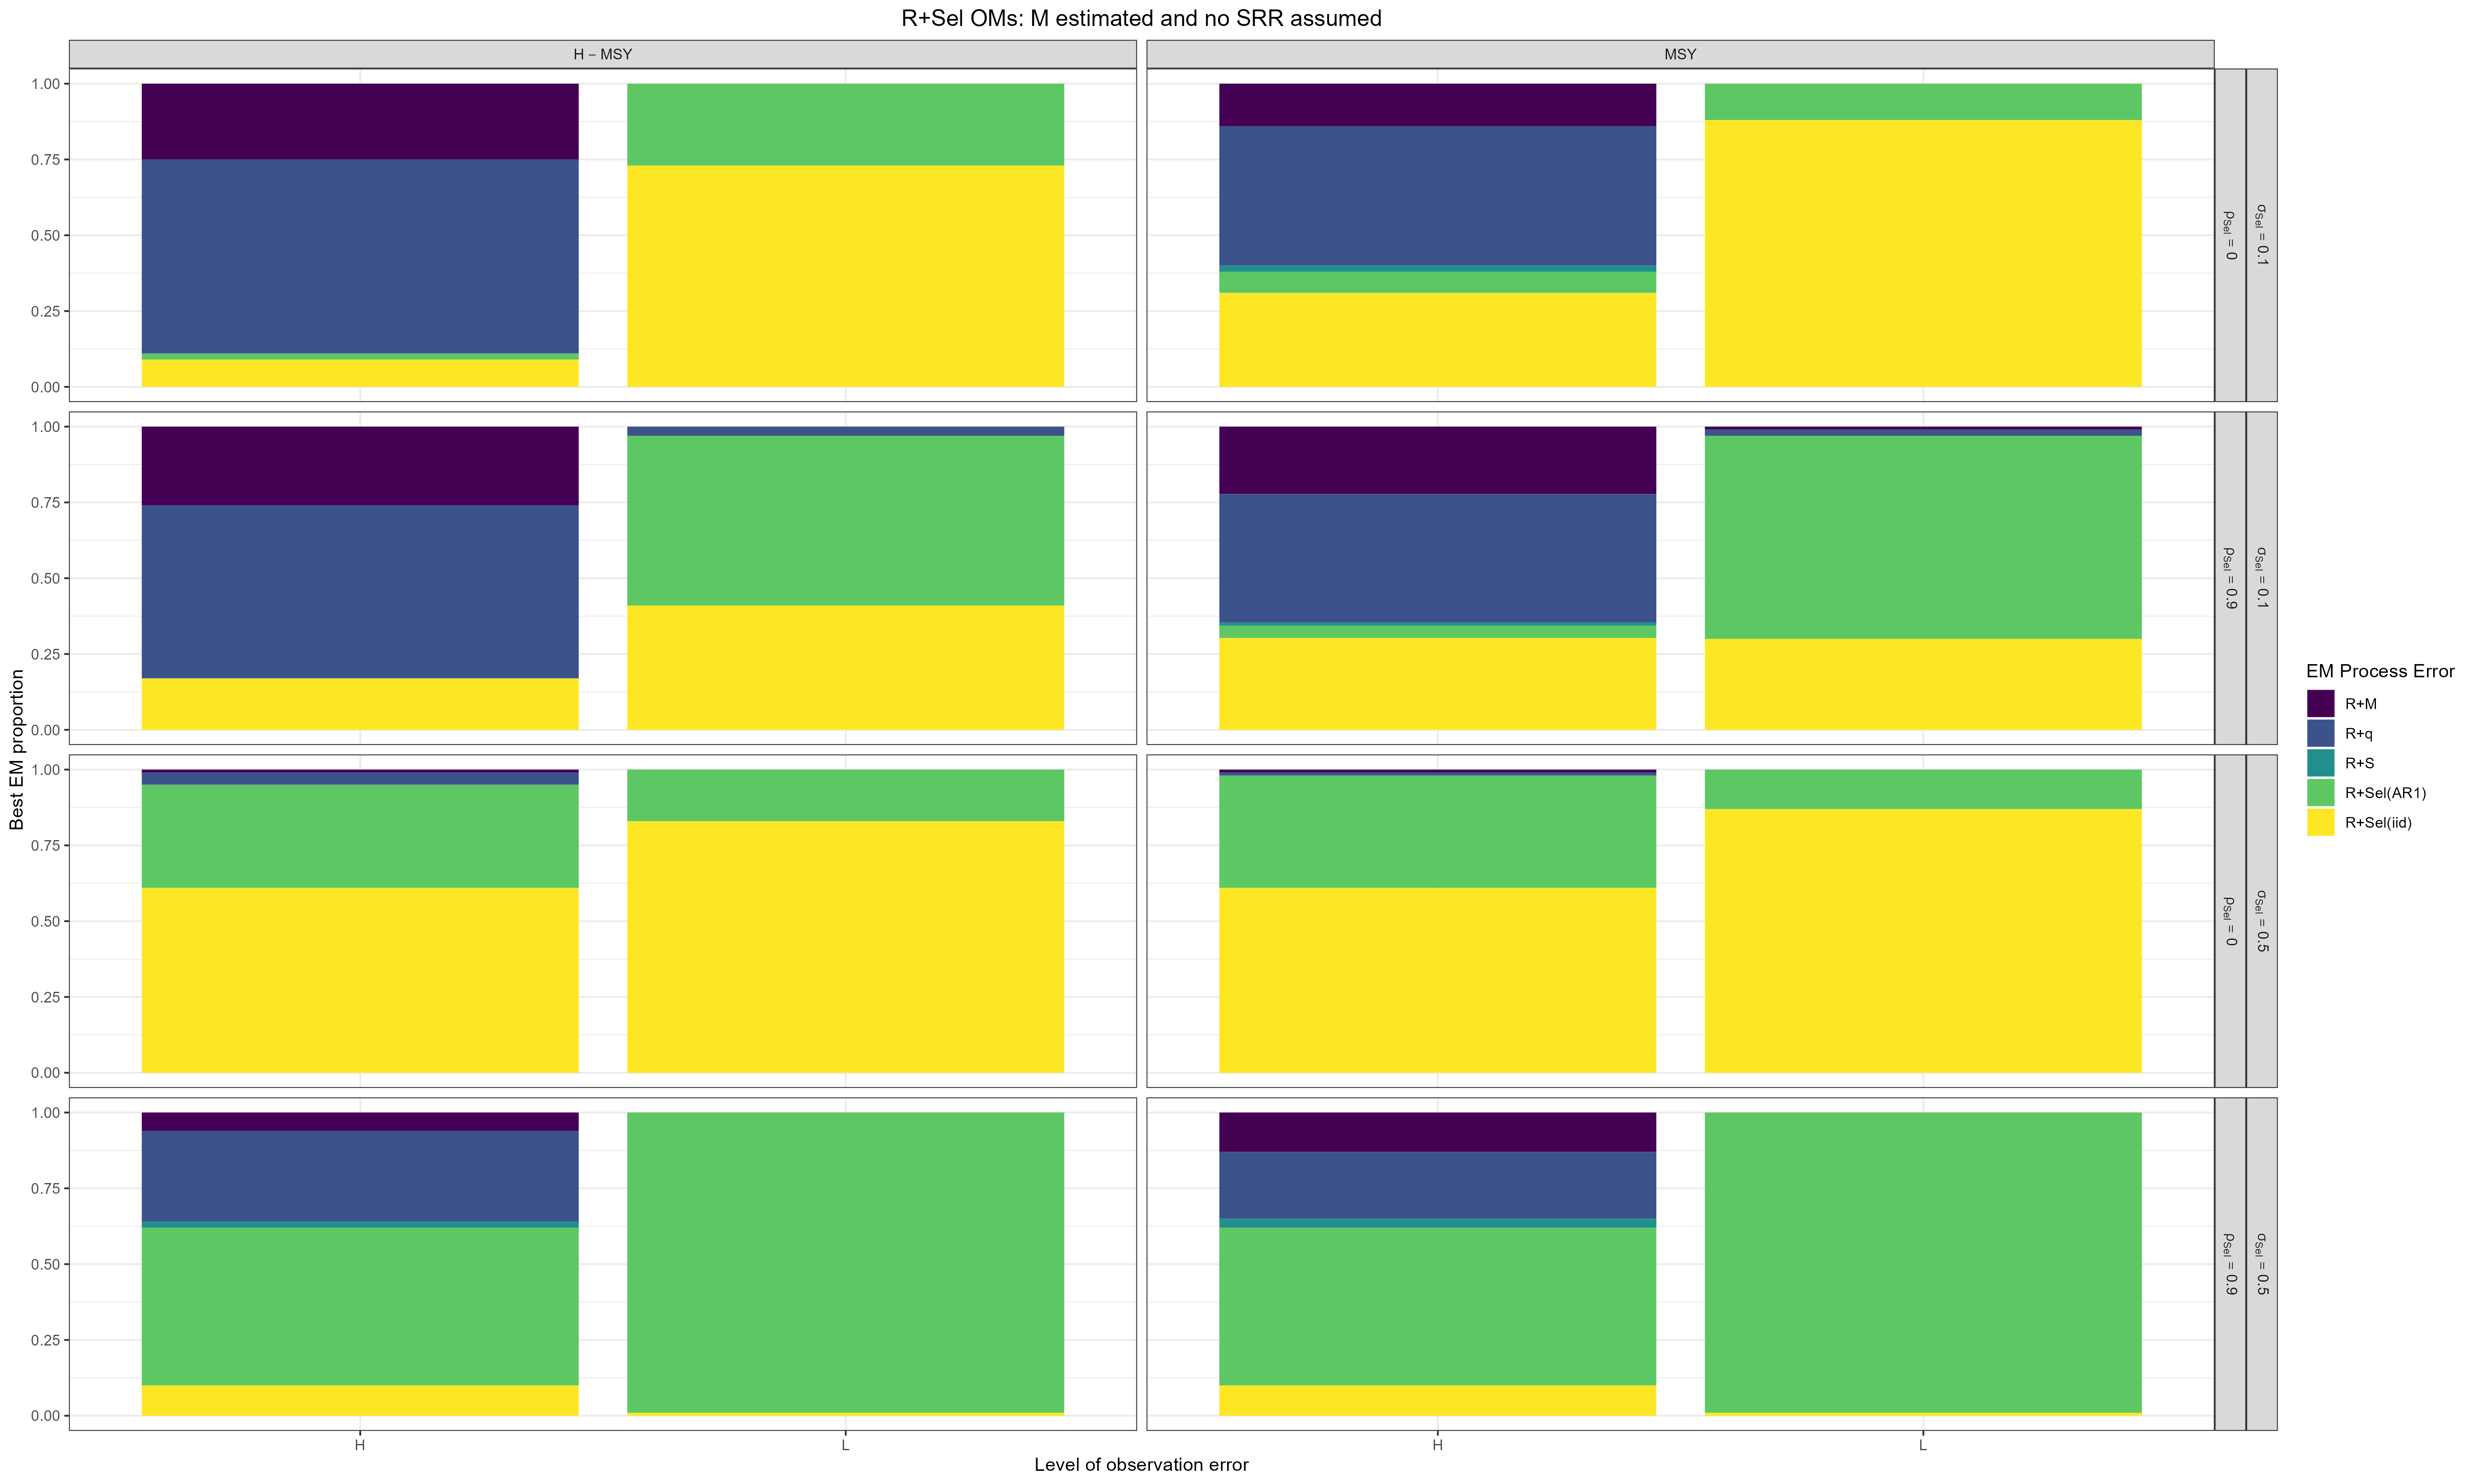
\includegraphics[width = \textwidth]{Sel_om_proportion_best_aic_R_ME.png}
\end{center}
\end{figure}
\end{landscape}

\begin{landscape}
\begin{figure}
\caption{Proportion of simulated data sets from OMs with R+Sel process errors where fitted estimating models had lowest marginal AIC. All estimating models estimate a stock-recruit relationship and and M is fixed at the true value.} \label{Sel_om_proportion_best_aic_SR_MF}
\begin{center}
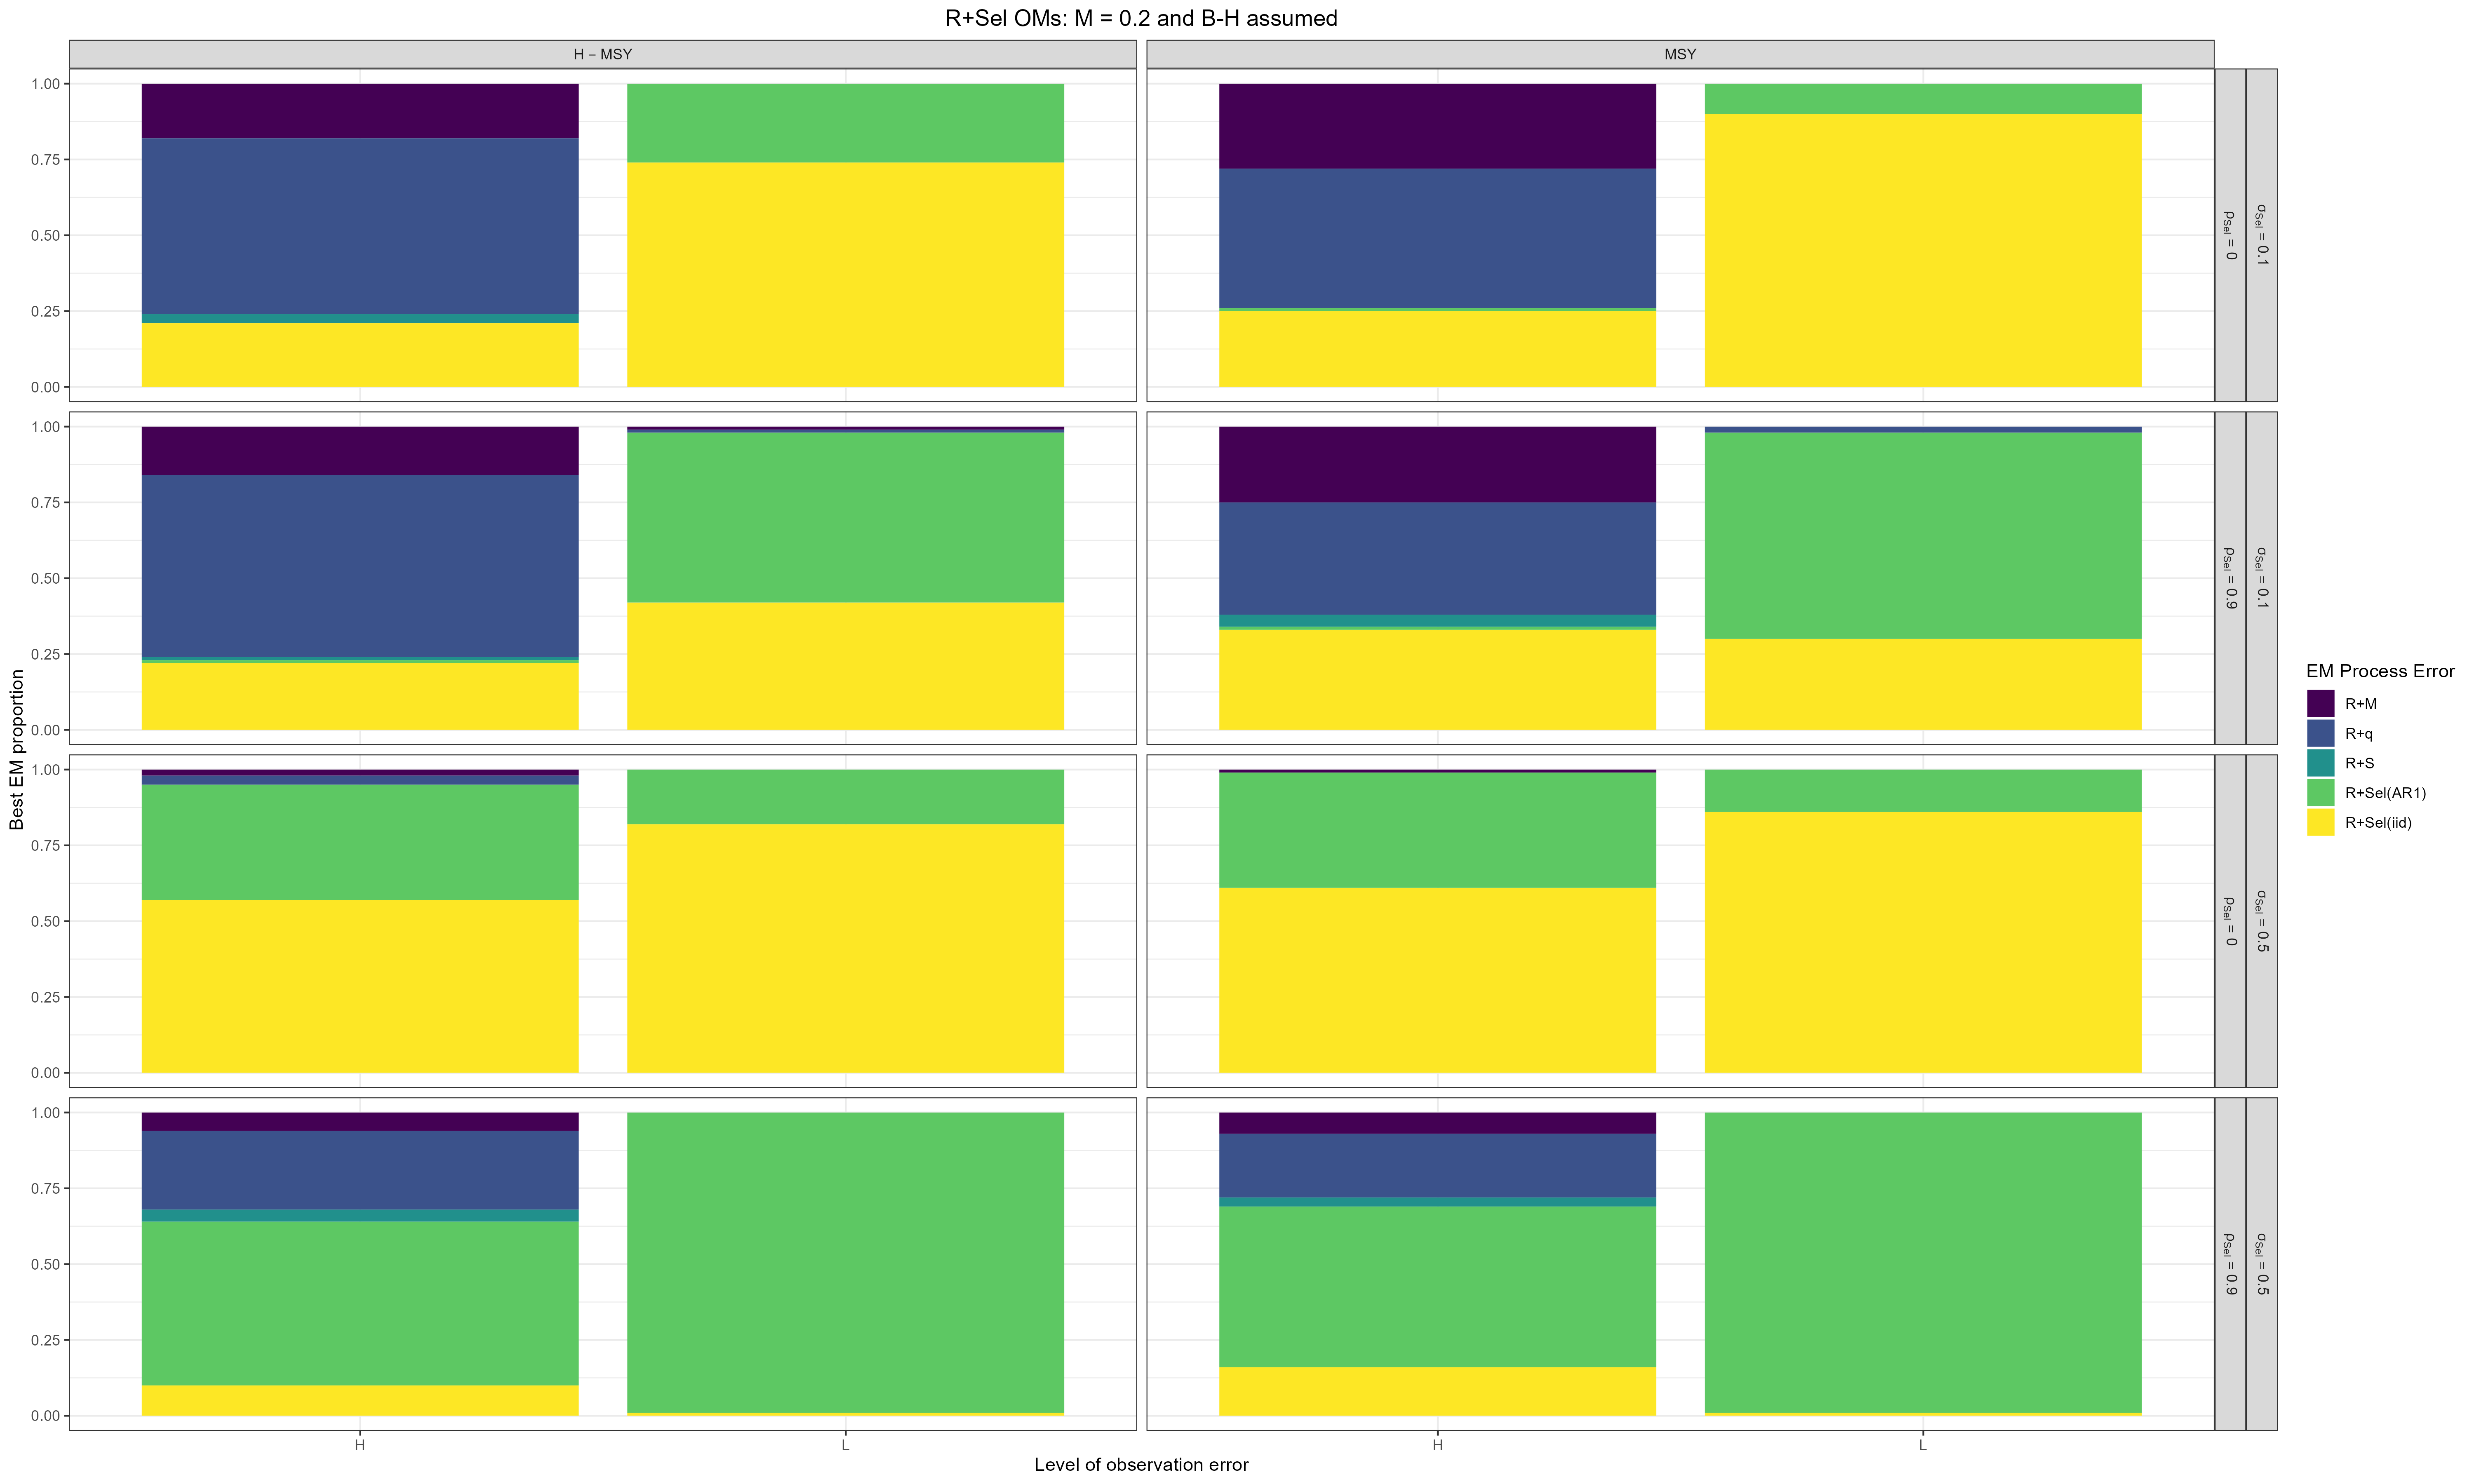
\includegraphics[width = \textwidth]{Sel_om_proportion_best_aic_SR_MF.png}
\end{center}
\end{figure}
\end{landscape}

\begin{landscape}
\begin{figure}
\caption{Proportion of simulated data sets from OMs with R+Sel process errors where fitted estimating models had lowest marginal AIC. All estimating models estimate a stock-recruit relationship and and M is estimated.} \label{Sel_om_proportion_best_aic_SR_ME}
\begin{center}
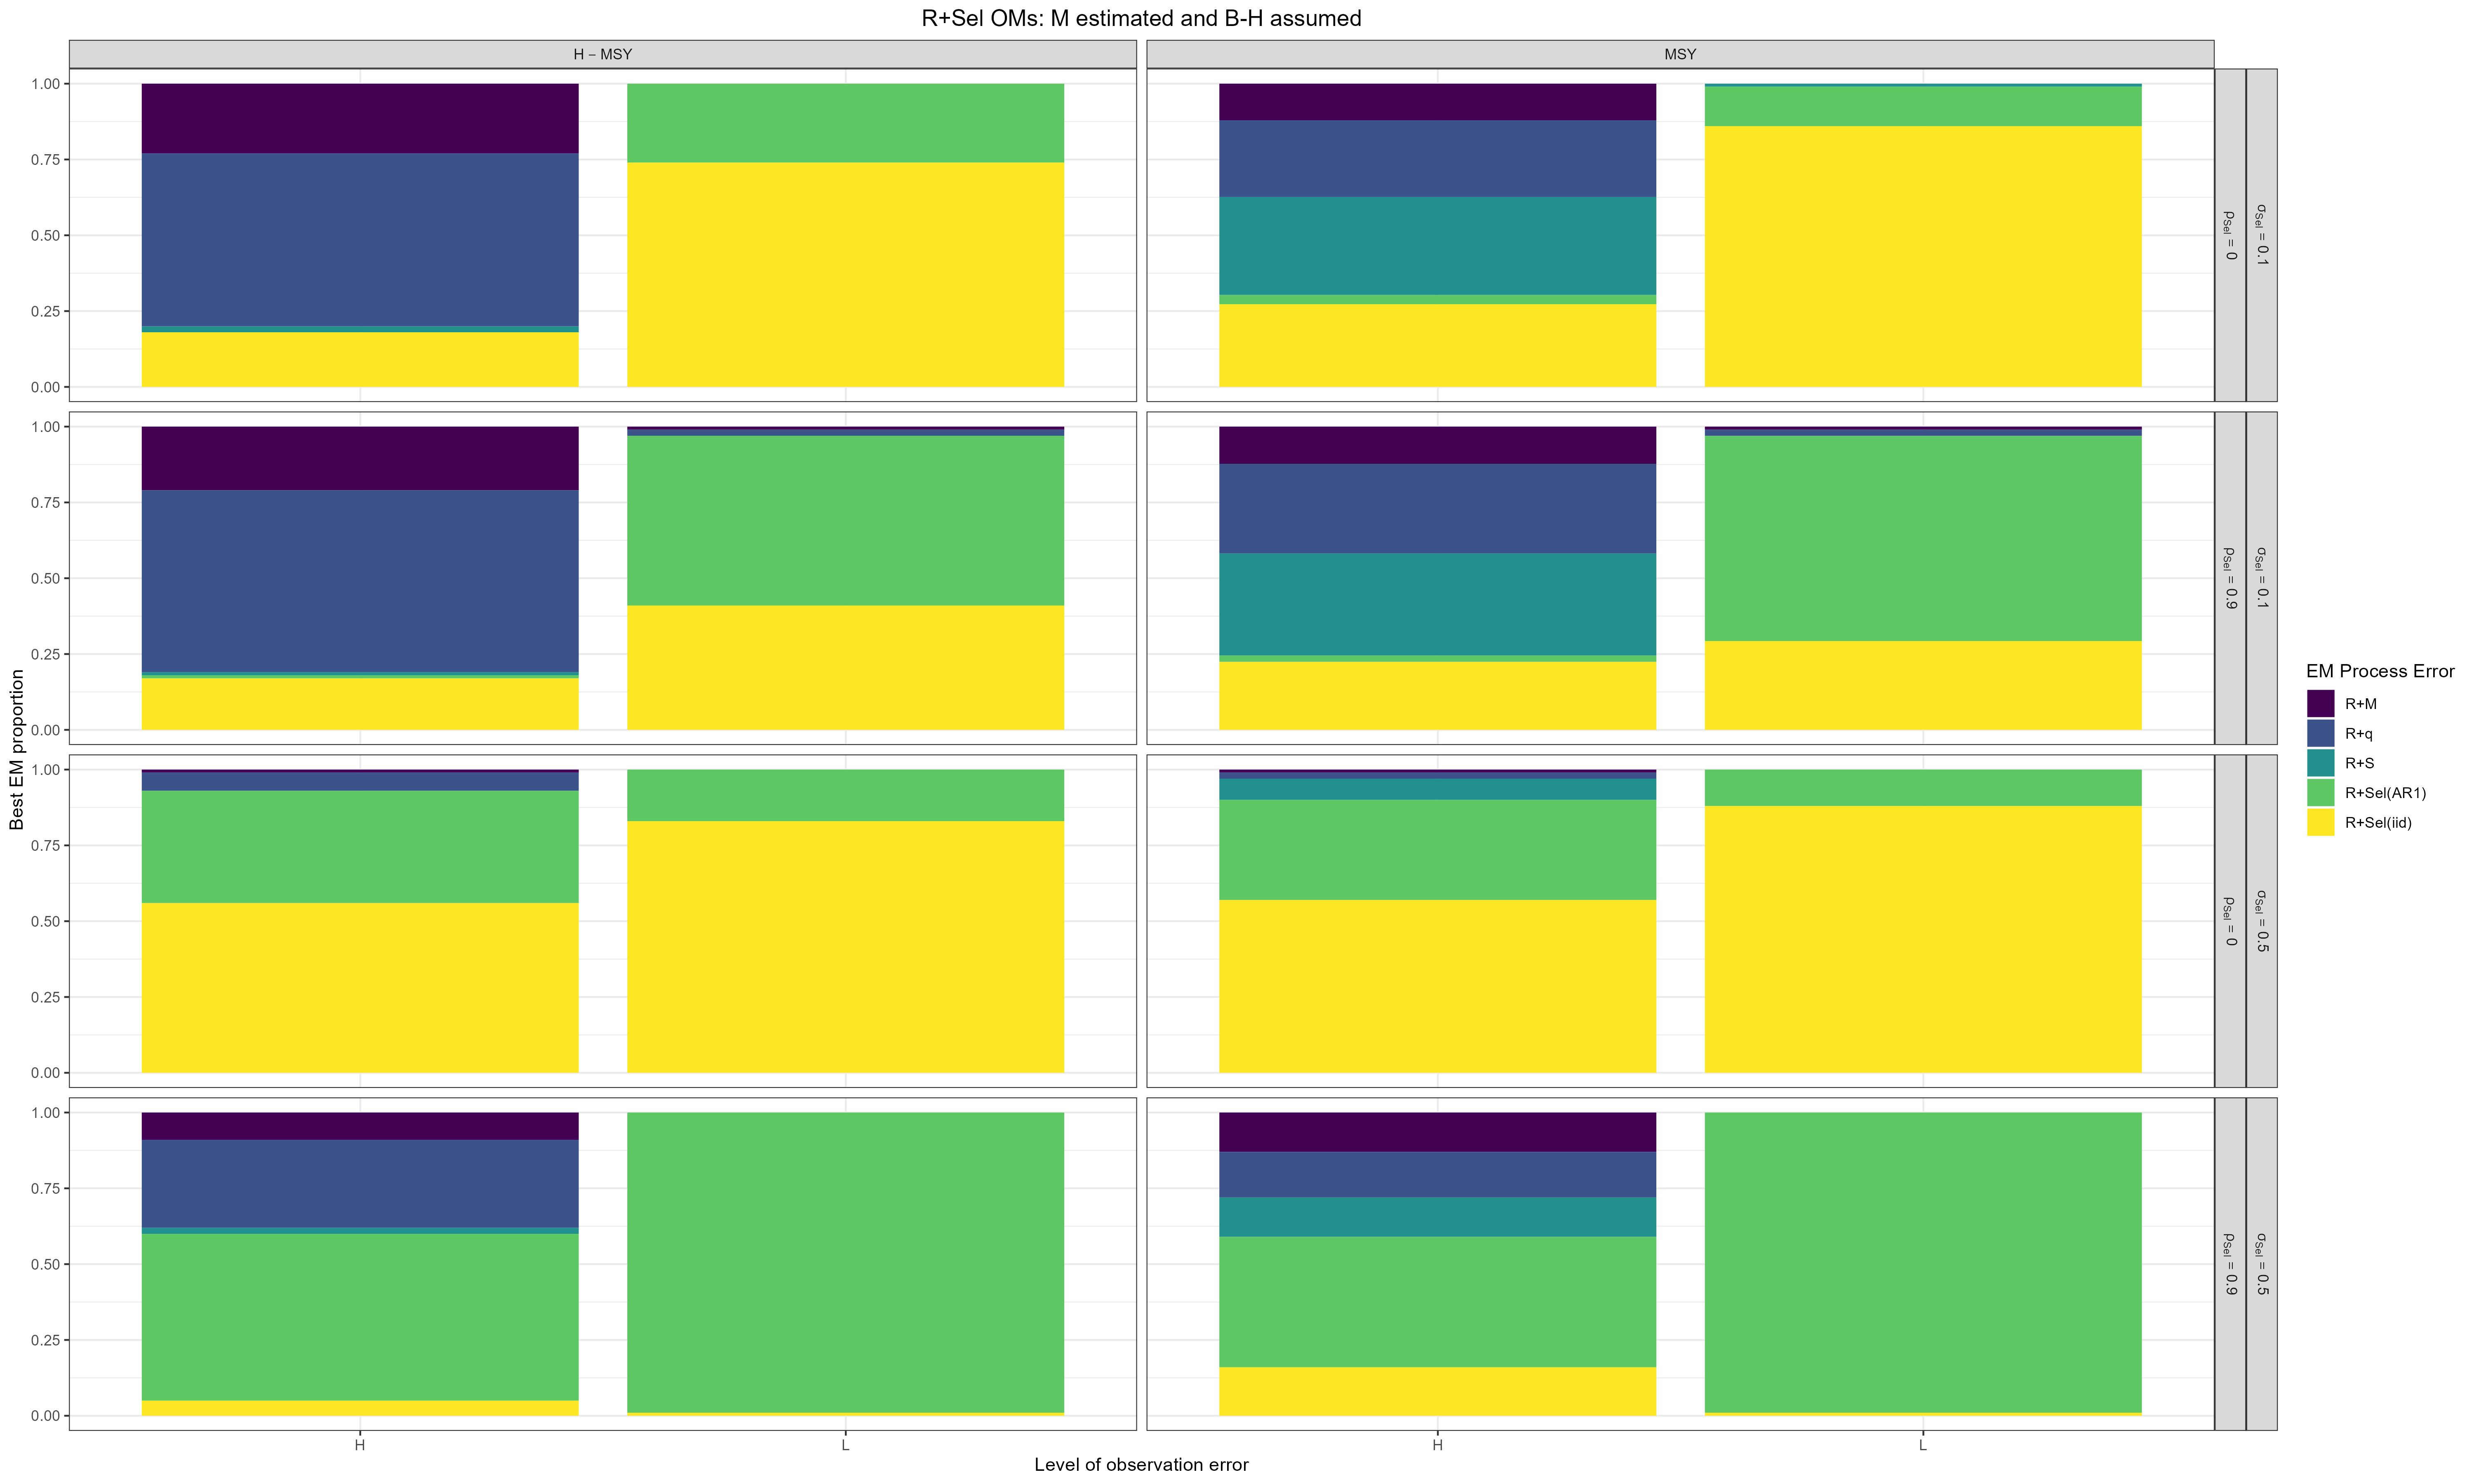
\includegraphics[width = \textwidth]{Sel_om_proportion_best_aic_SR_ME.png}
\end{center}
\end{figure}
\end{landscape}

\hypertarget{rq-operating-models-1}{%
\subsubsection*{R+q operating models}\label{rq-operating-models-1}}
\addcontentsline{toc}{subsubsection}{R+q operating models}

Figures \ref{q_om_proportion_best_aic_R_MF} to
\ref{q_om_proportion_best_aic_SR_ME}

\begin{landscape}
\begin{figure}
\caption{Proportion of simulated data sets from OMs with R+q process errors where fitted estimating models had lowest marginal AIC. All estimating models estimate mean recruitment rather than a stock-recruit relationship and and M is fixed at the true value.} \label{q_om_proportion_best_aic_R_MF}
\begin{center}
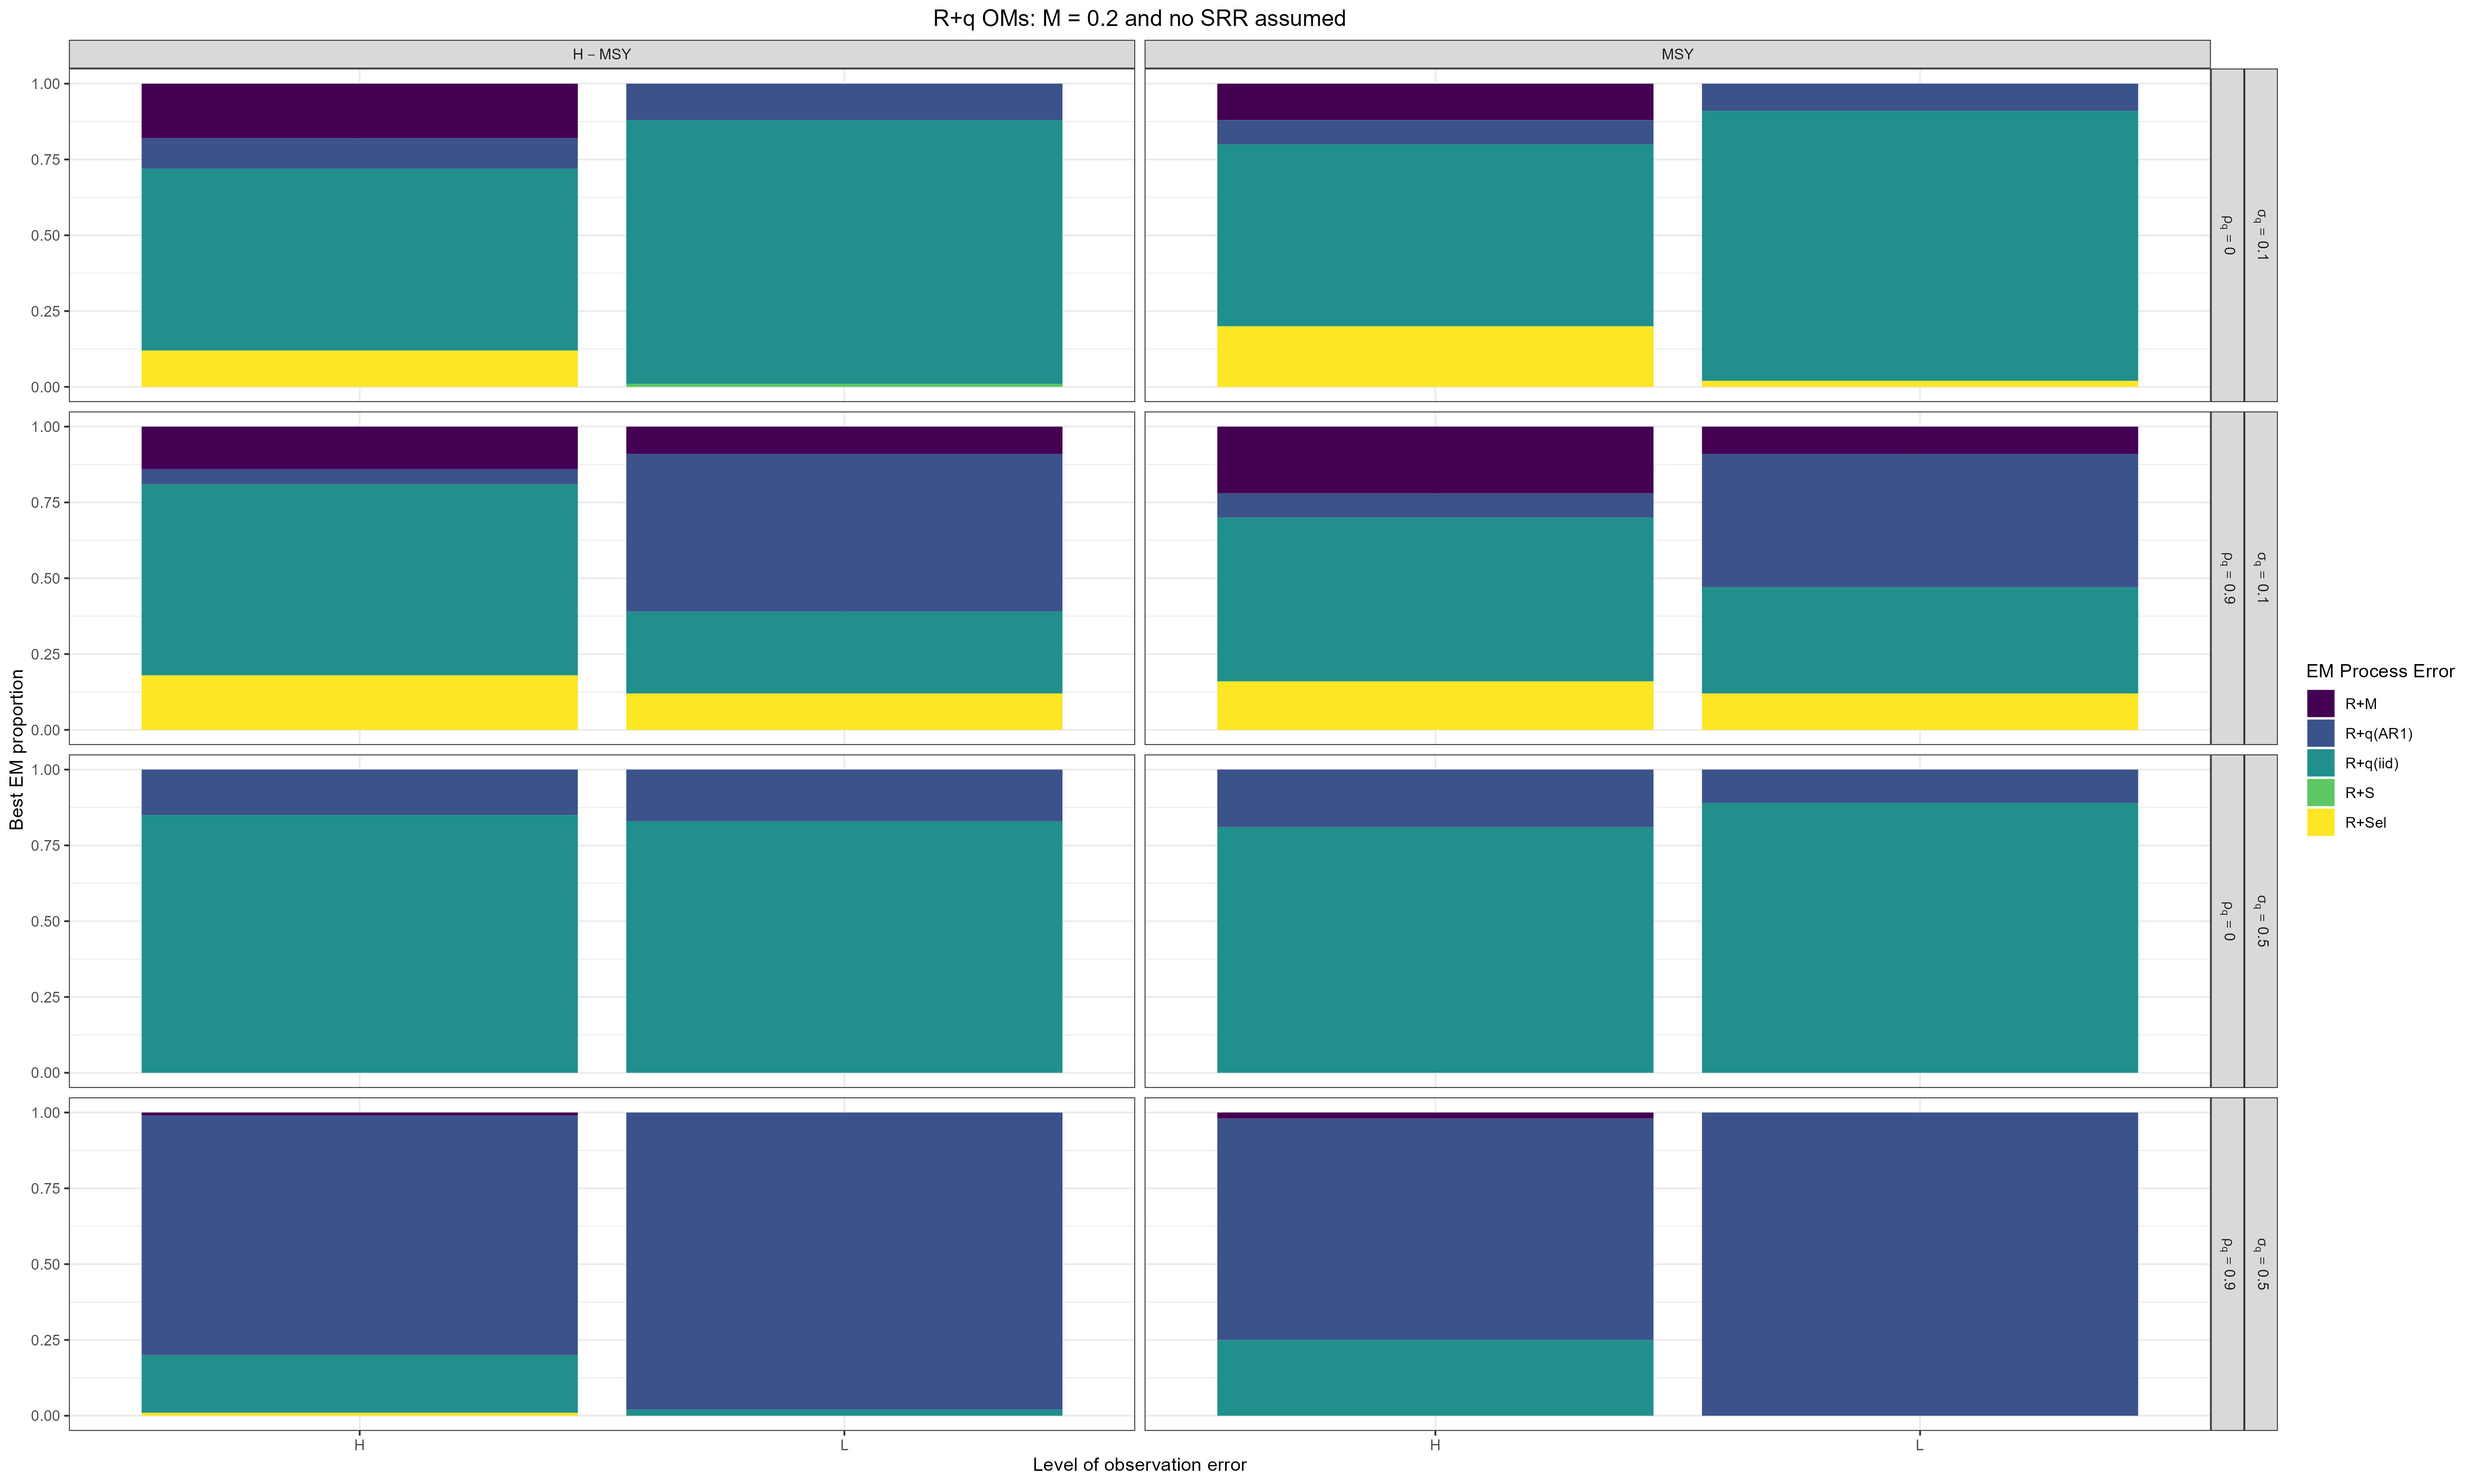
\includegraphics[width = \textwidth]{q_om_proportion_best_aic_R_MF.png}
\end{center}
\end{figure}
\end{landscape}

\begin{landscape}
\begin{figure}
\caption{Proportion of simulated data sets from OMs with R+q process errors where fitted estimating models had lowest marginal AIC. All estimating models estimate mean recruitment rather than a stock-recruit relationship and and M is estimated.} \label{q_om_proportion_best_aic_R_ME}
\begin{center}
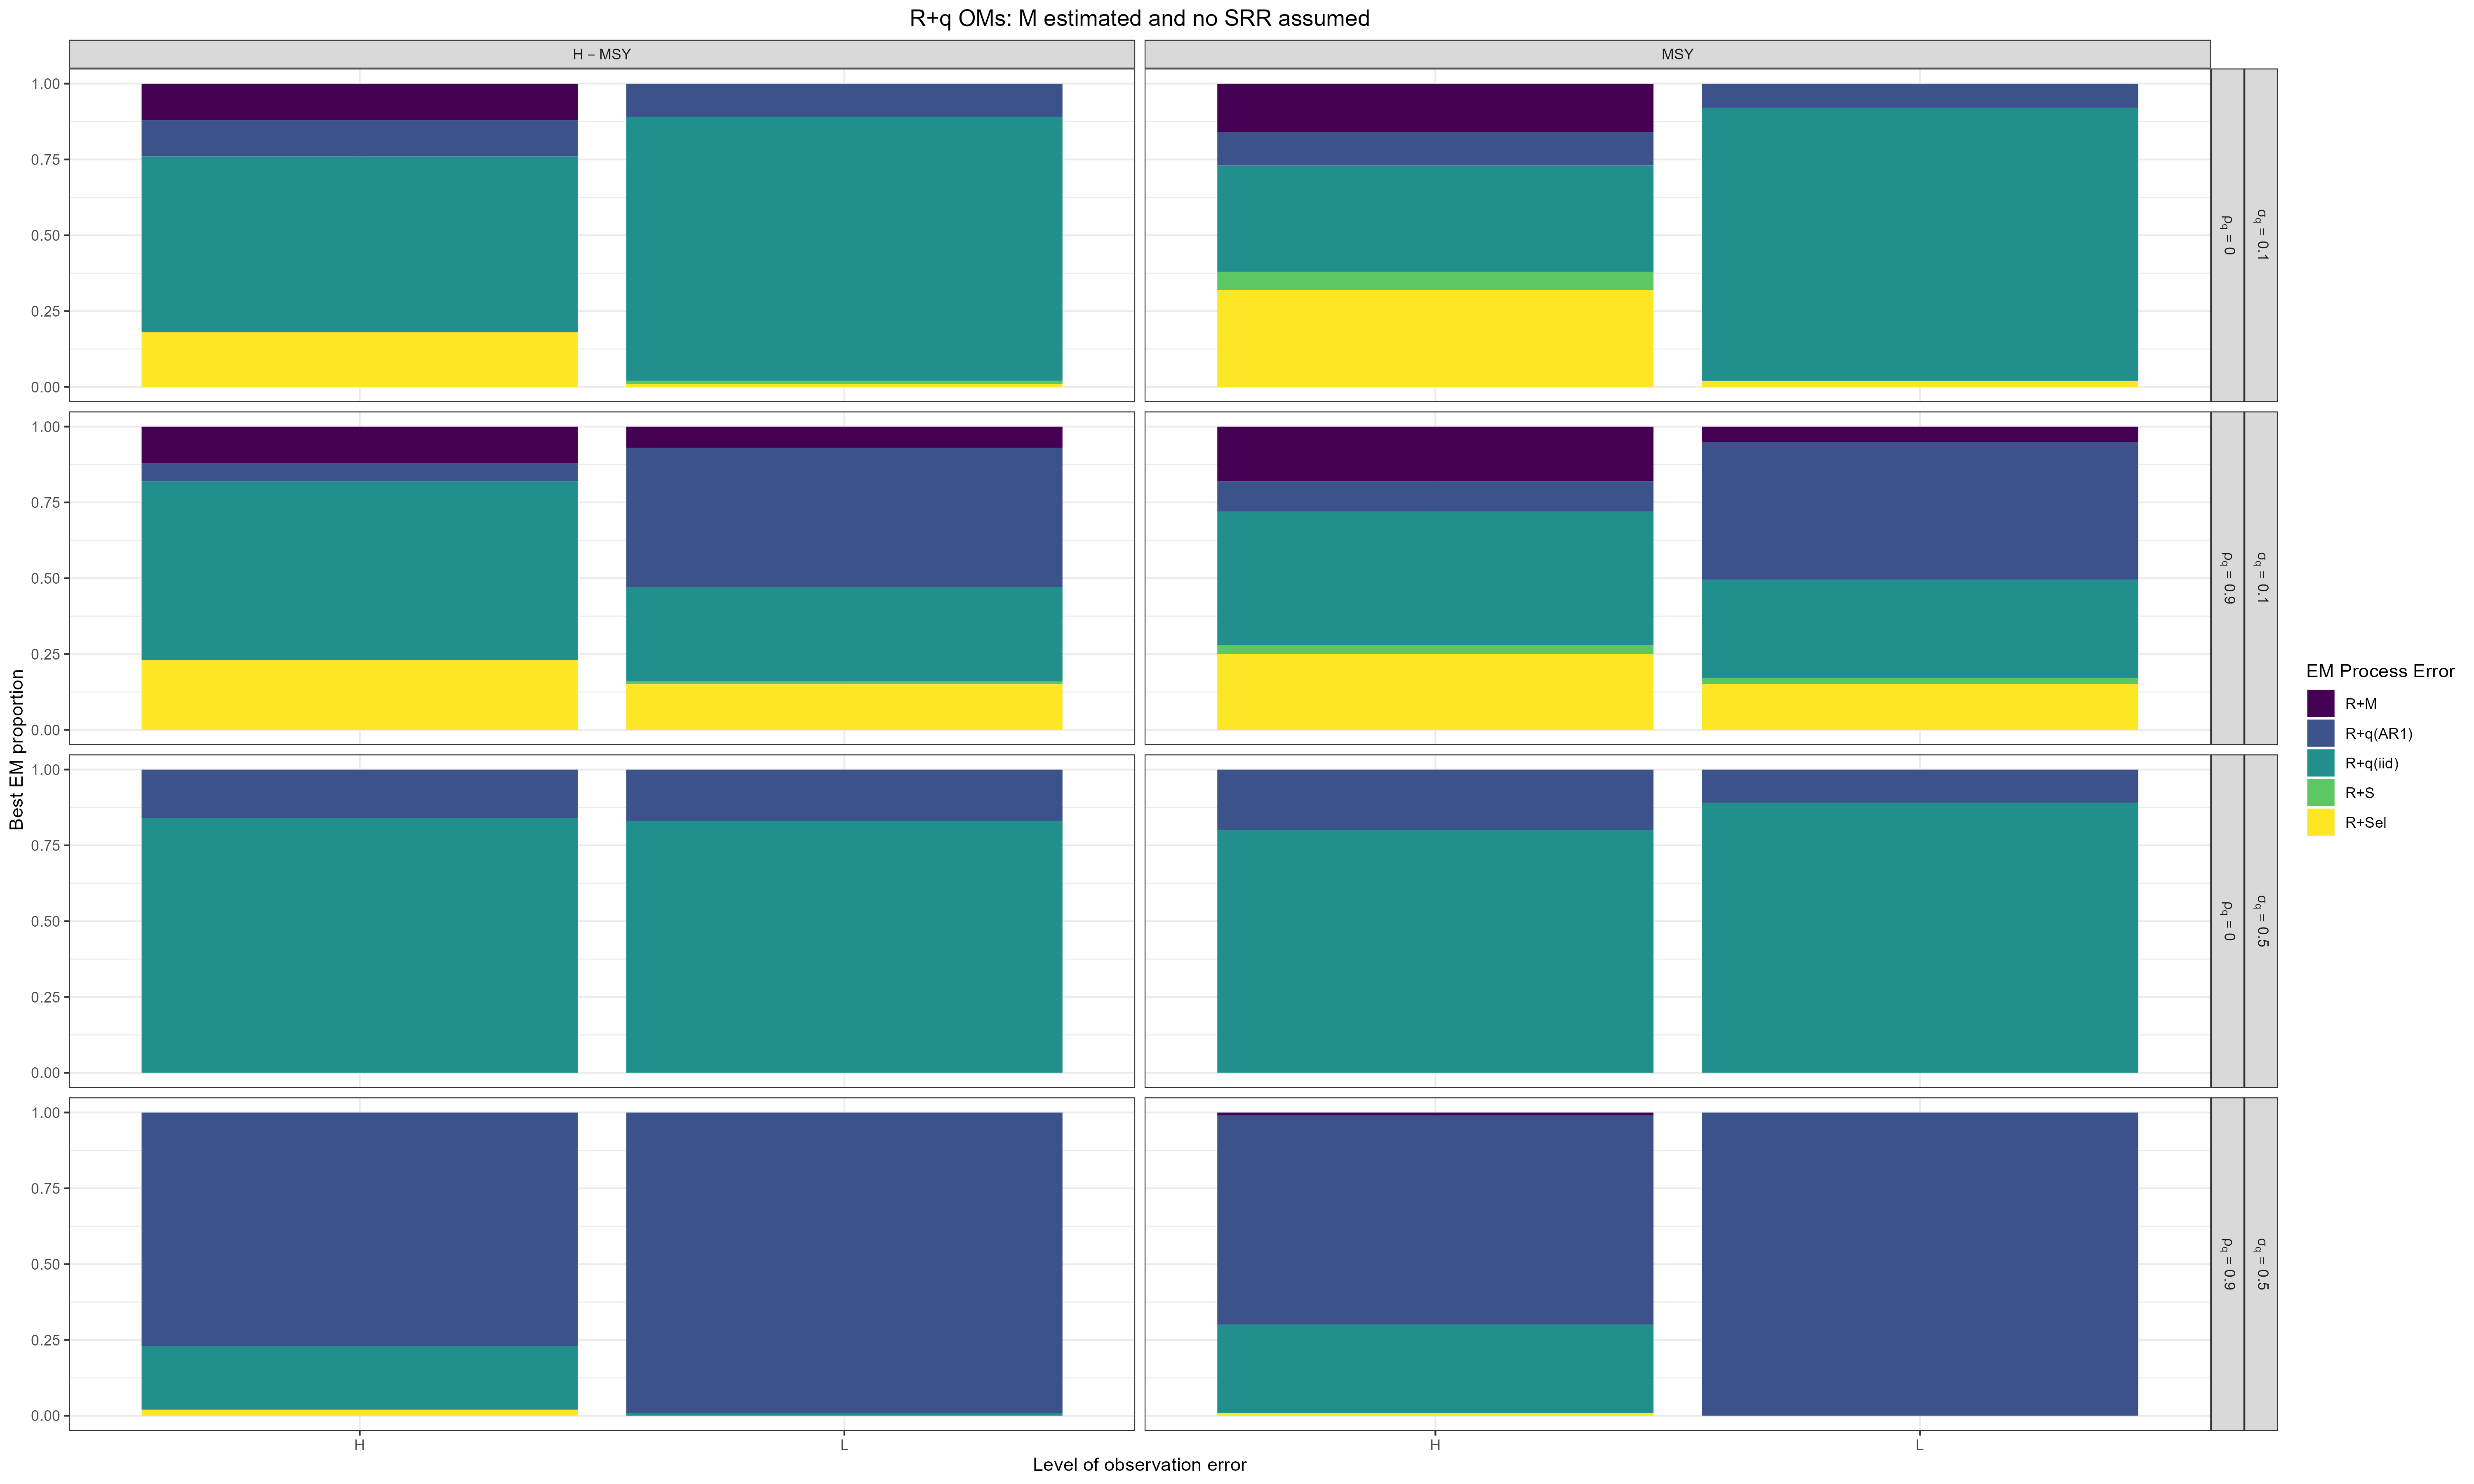
\includegraphics[width = \textwidth]{q_om_proportion_best_aic_R_ME.png}
\end{center}
\end{figure}
\end{landscape}

\begin{landscape}
\begin{figure}
\caption{Proportion of simulated data sets from OMs with R+q process errors where fitted estimating models had lowest marginal AIC. All estimating models estimate a stock-recruit relationship and and M is fixed at the true value.} \label{q_om_proportion_best_aic_SR_MF}
\begin{center}
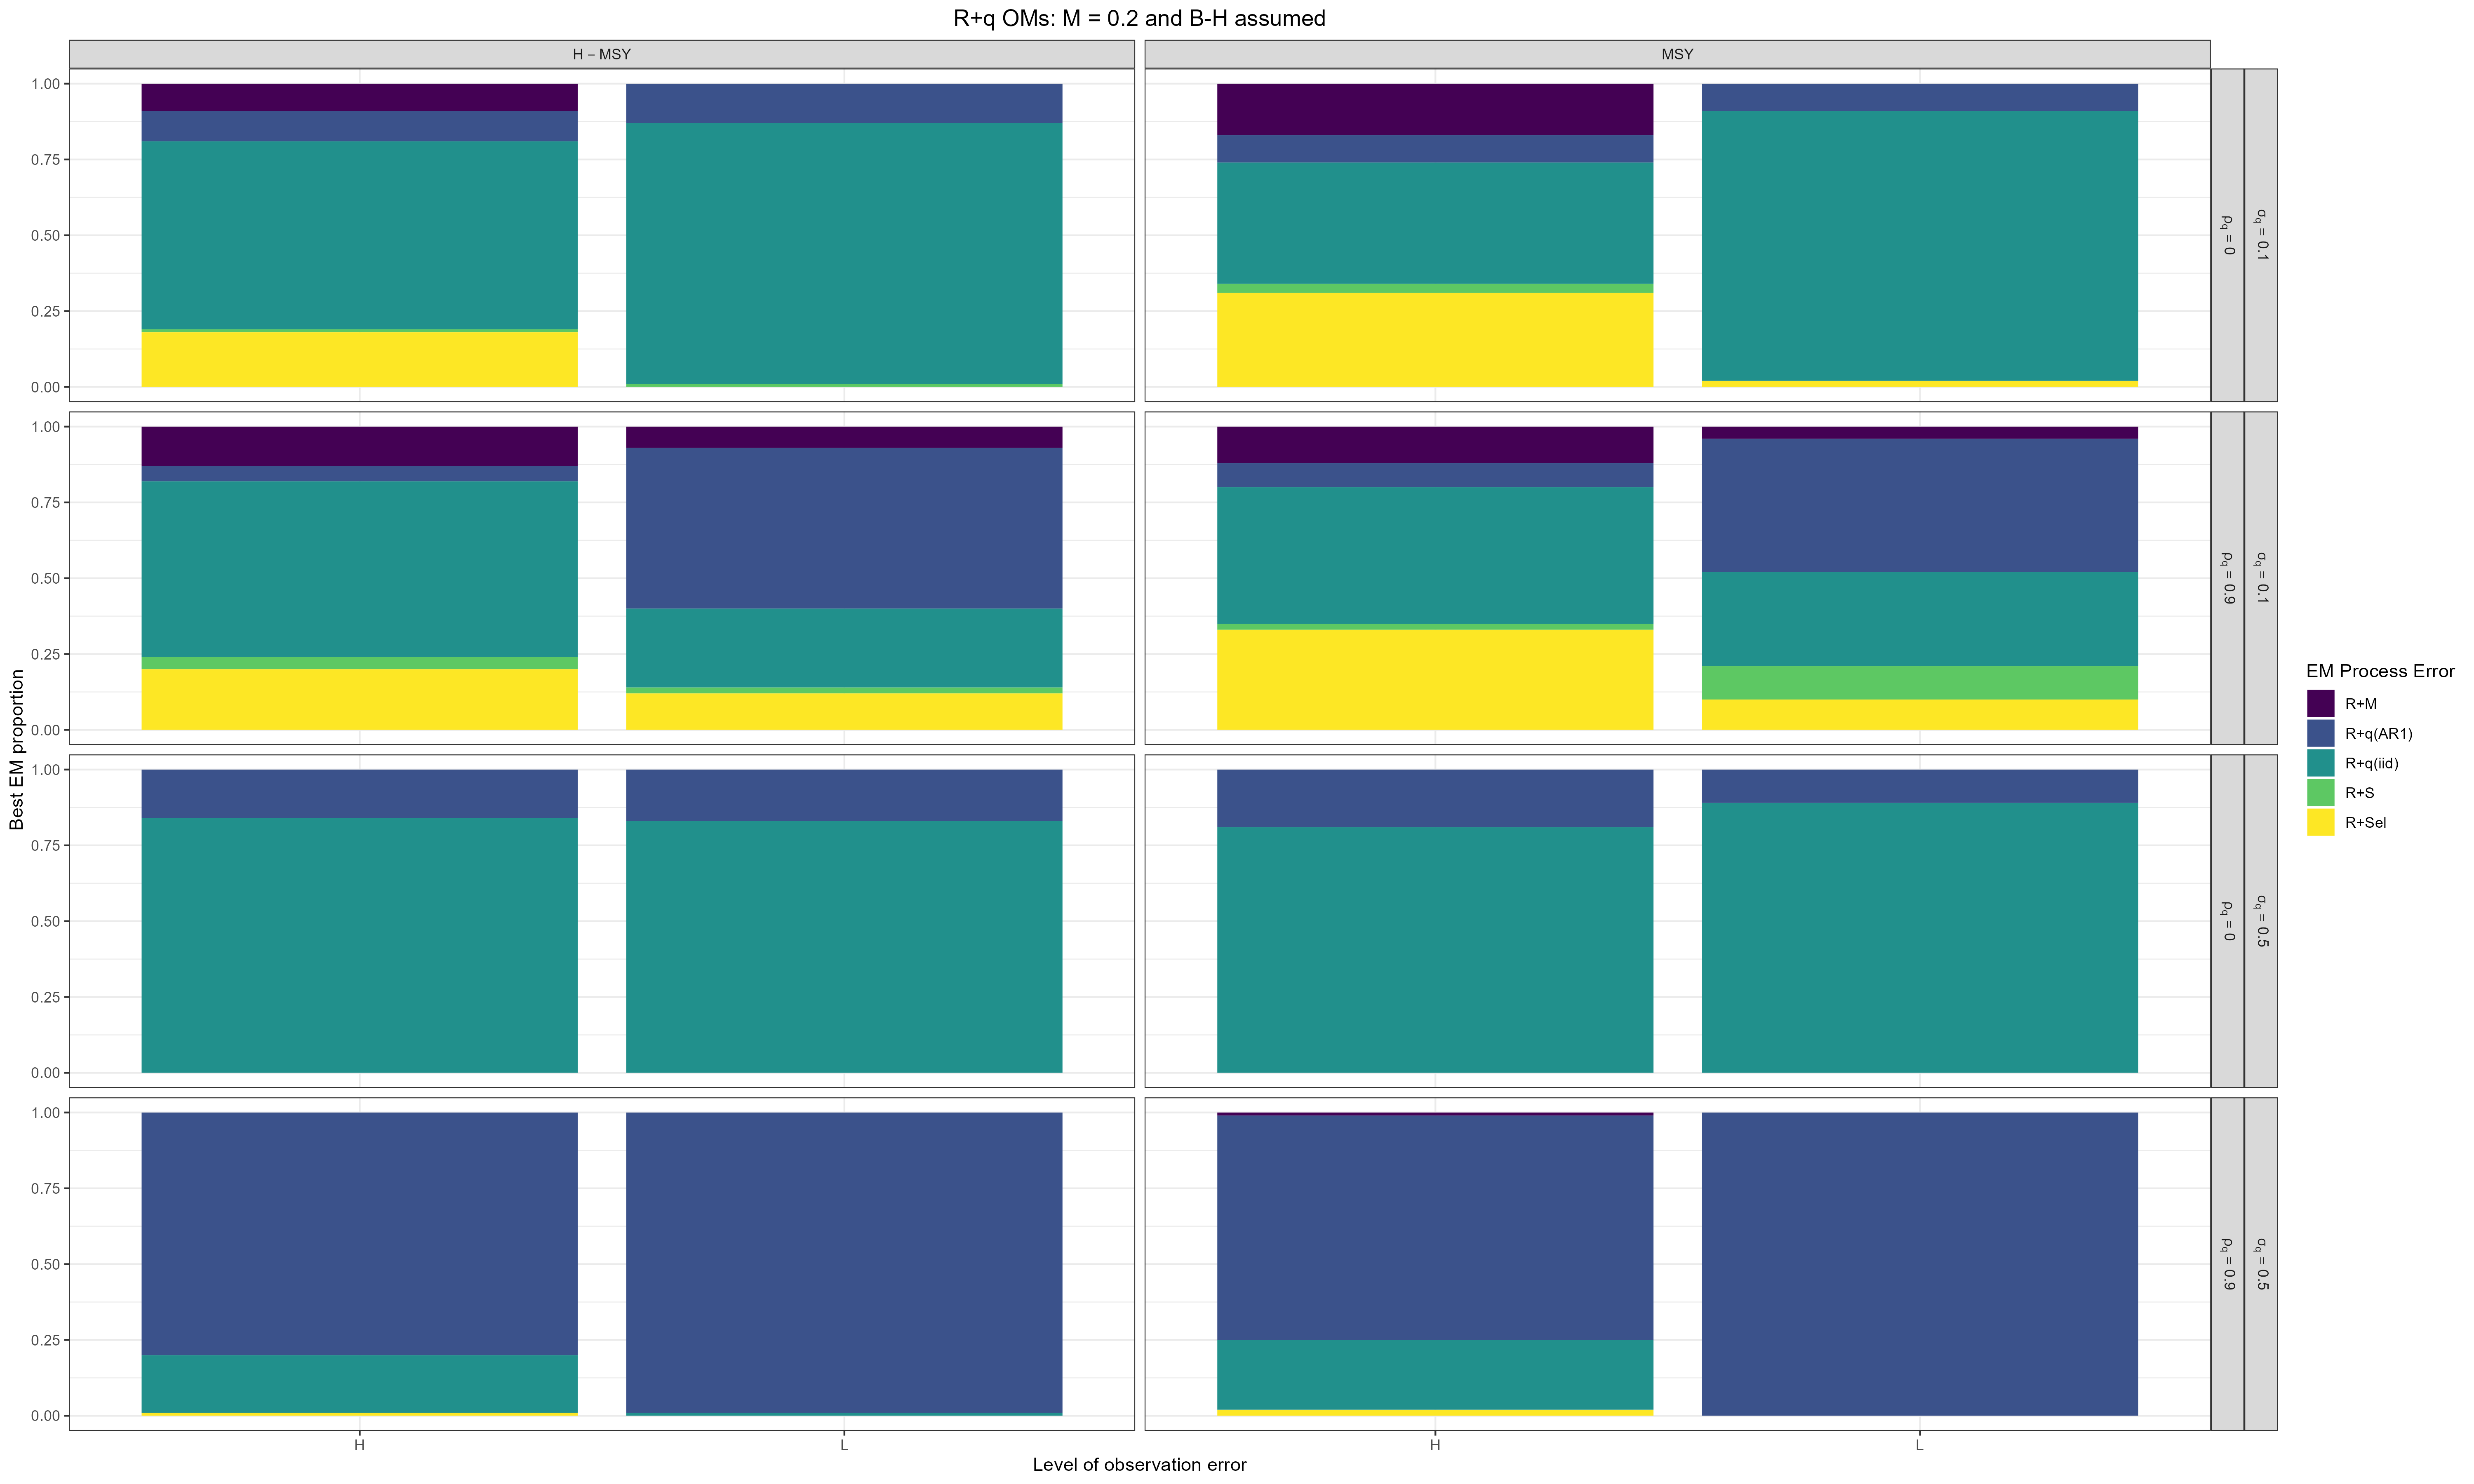
\includegraphics[width = \textwidth]{q_om_proportion_best_aic_SR_MF.png}
\end{center}
\end{figure}
\end{landscape}

\begin{landscape}
\begin{figure}
\caption{Proportion of simulated data sets from OMs with R+q process errors where fitted estimating models had lowest marginal AIC. All estimating models estimate a stock-recruit relationship and and M is estimated.} \label{q_om_proportion_best_aic_SR_ME}
\begin{center}
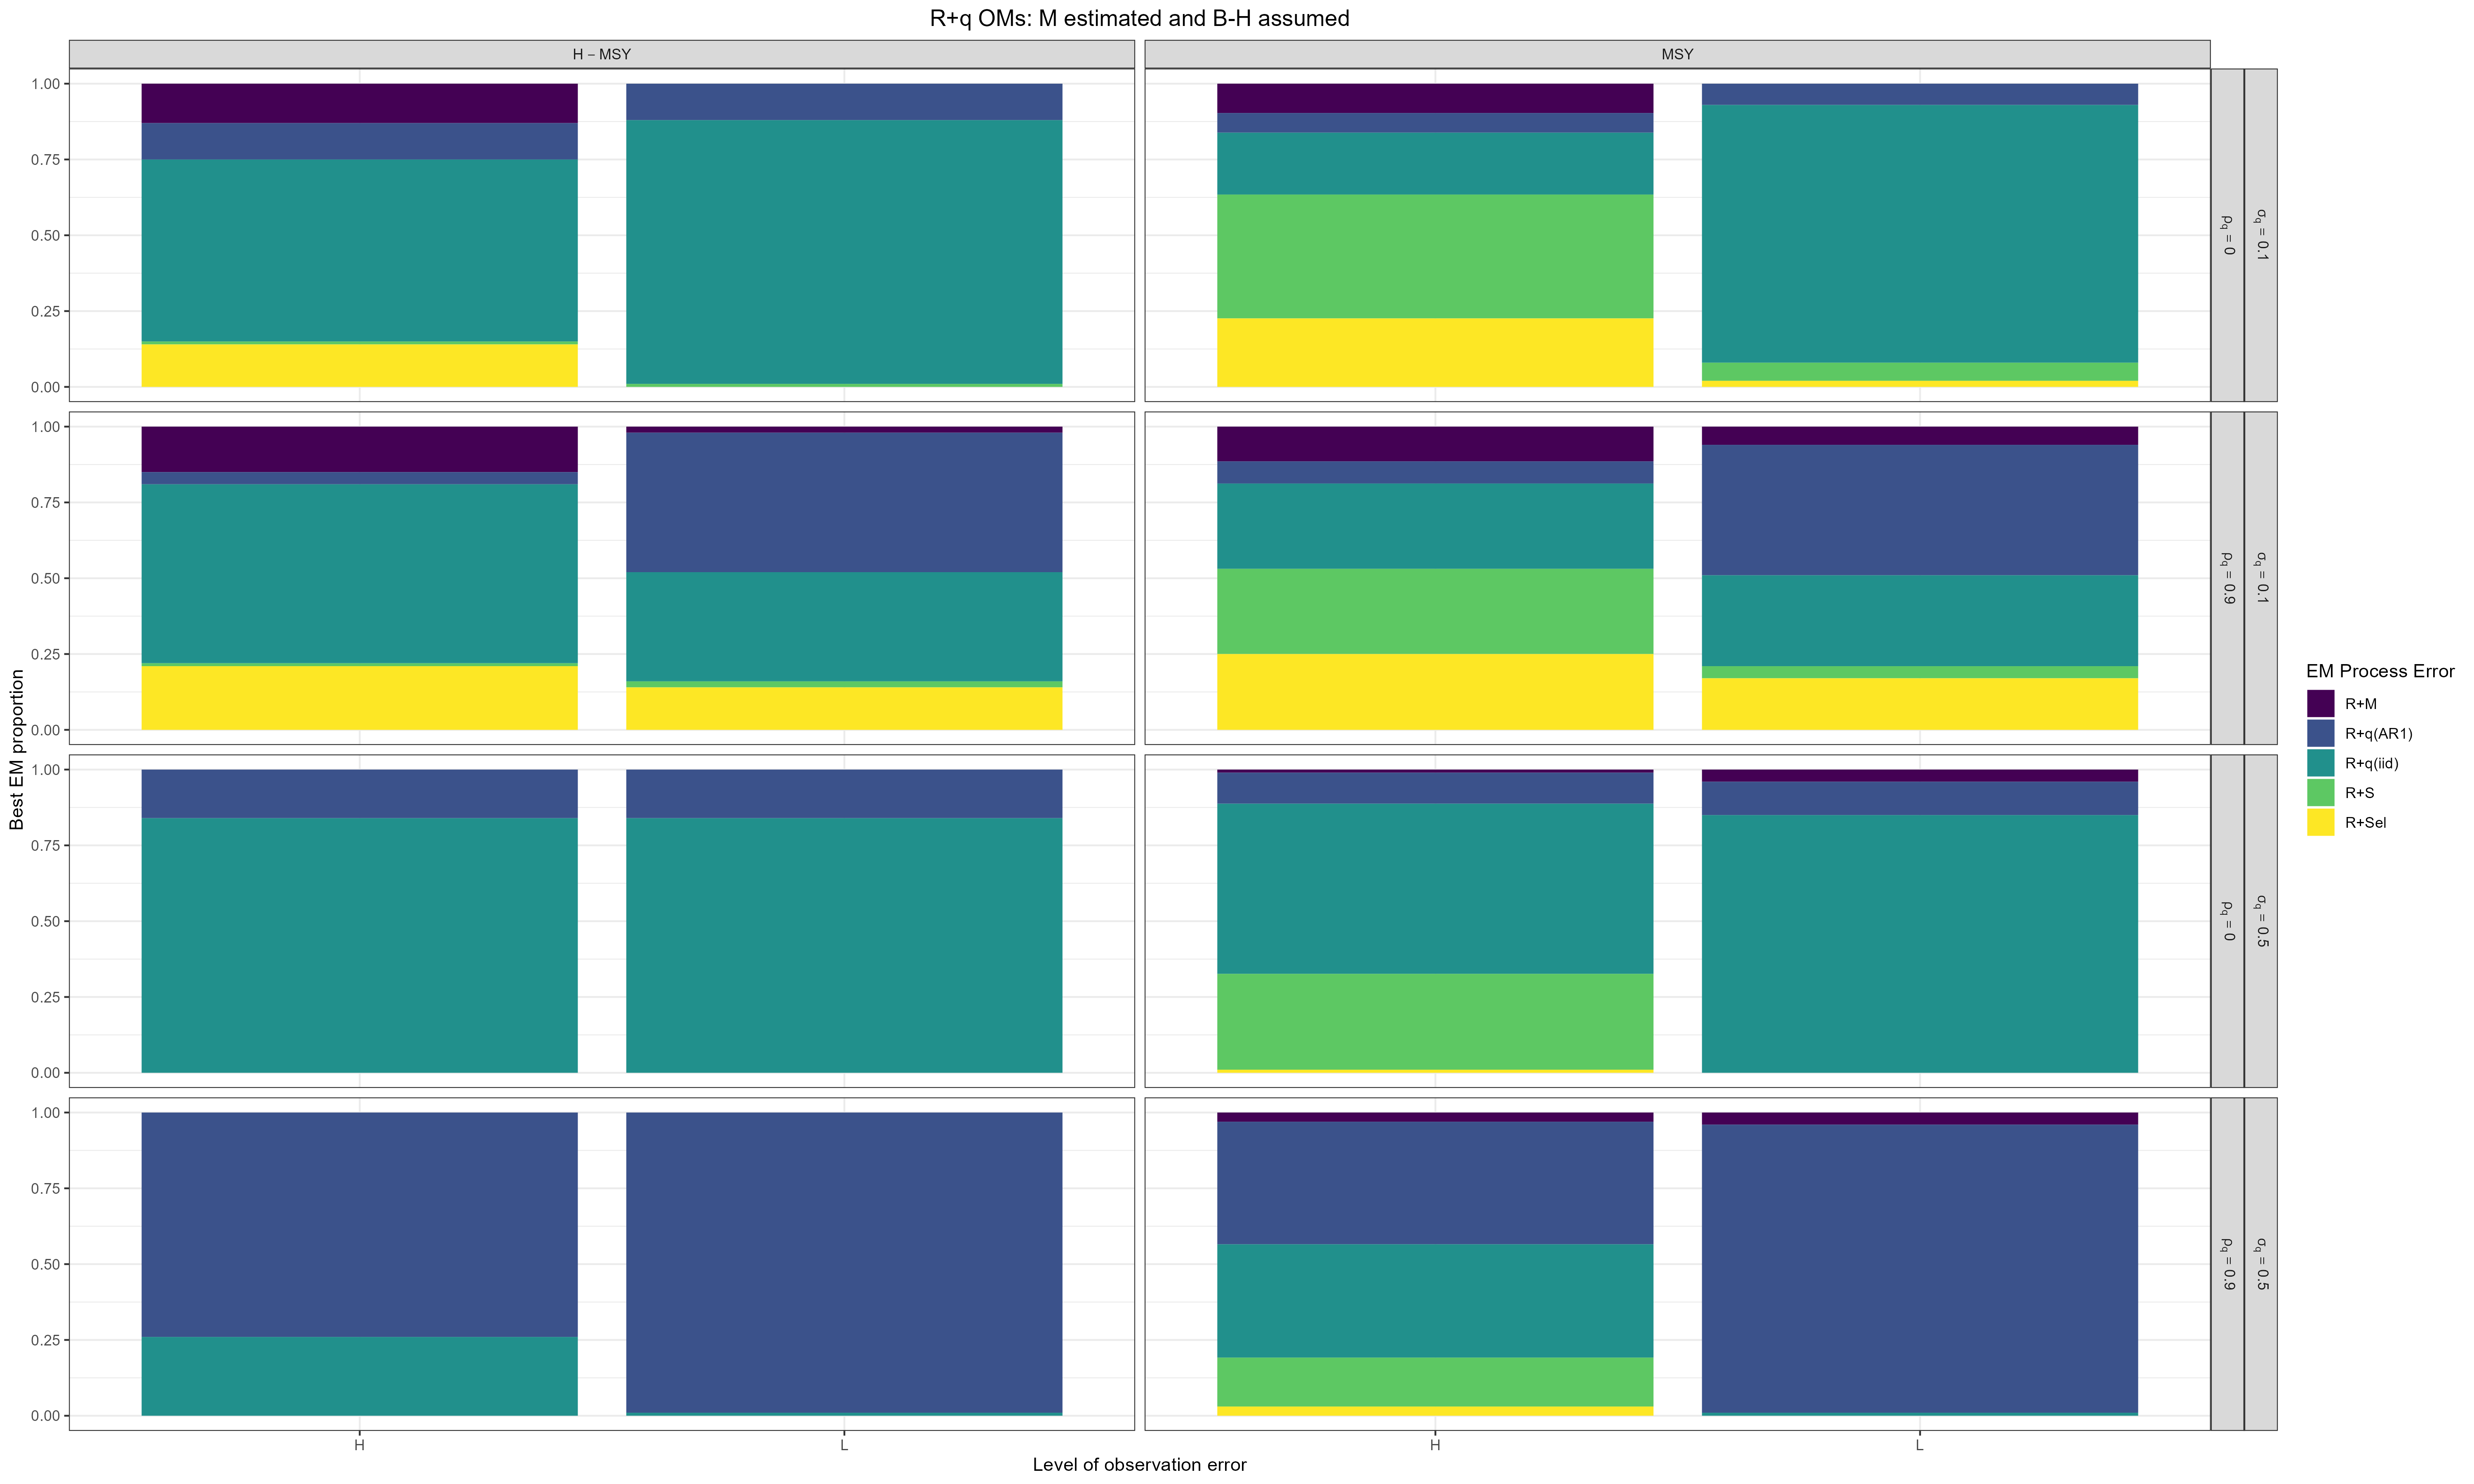
\includegraphics[width = \textwidth]{q_om_proportion_best_aic_SR_ME.png}
\end{center}
\end{figure}
\end{landscape}

\clearpage

\hypertarget{aic-performance-for-stock-recruit-relationship}{%
\subsection*{AIC performance for stock-recruit
relationship}\label{aic-performance-for-stock-recruit-relationship}}
\addcontentsline{toc}{subsection}{AIC performance for stock-recruit
relationship}

Tables of frequencies where AIC chooses correct stock-recruit assumption
imply poor performance of AIC, but figures showing effect of variation
in SSB demonstrate that large variation in SSB is needed to reduce Type
II errors for marginal AIC.

\hypertarget{r-rs-operating-models-2}{%
\subsubsection*{R, R+S operating models}\label{r-rs-operating-models-2}}
\addcontentsline{toc}{subsubsection}{R, R+S operating models}

\begin{table}
\caption{Operating models and estimation models all assume matching R or R+S process error structure, estimating models assume mean recruitment or a B-H stock recruit relationship and M is either fixed at the true value or estimated.}
{\begin{center}
\begin{tabular}{rrrrrrrr}
\hline\hline
\multicolumn{1}{c}{$\sigma_R$}&\multicolumn{1}{c}{$\sigma_N$}&\multicolumn{1}{c}{F-history}&\multicolumn{1}{c}{Obs Error}&\multicolumn{1}{c}{R (M fix)}&\multicolumn{1}{c}{BH (M fix)}&\multicolumn{1}{c}{R (M est)}&\multicolumn{1}{c}{BH (M est)}\tabularnewline
\hline
$0.5$&$$&H-MSY&L&$46$&$54$&$45$&$55$\tabularnewline
$1.5$&$$&H-MSY&L&$81$&$19$&$81$&$19$\tabularnewline
$0.5$&$$&MSY&L&$94$&$ 6$&$94$&$ 6$\tabularnewline
$1.5$&$$&MSY&L&$91$&$ 9$&$92$&$ 8$\tabularnewline
$0.5$&$$&H-MSY&H&$52$&$48$&$56$&$44$\tabularnewline
$1.5$&$$&H-MSY&H&$82$&$18$&$81$&$19$\tabularnewline
$0.5$&$$&MSY&H&$91$&$ 9$&$92$&$ 8$\tabularnewline
$1.5$&$$&MSY&H&$90$&$10$&$91$&$ 9$\tabularnewline
$0.5$&$0.25$&H-MSY&L&$43$&$57$&$45$&$55$\tabularnewline
$1.5$&$0.25$&H-MSY&L&$84$&$16$&$84$&$16$\tabularnewline
$0.5$&$0.50$&H-MSY&L&$30$&$70$&$29$&$71$\tabularnewline
$1.5$&$0.50$&H-MSY&L&$78$&$22$&$78$&$22$\tabularnewline
$0.5$&$0.25$&MSY&L&$84$&$16$&$84$&$16$\tabularnewline
$1.5$&$0.25$&MSY&L&$90$&$10$&$91$&$ 9$\tabularnewline
$0.5$&$0.50$&MSY&L&$68$&$32$&$68$&$32$\tabularnewline
$1.5$&$0.50$&MSY&L&$91$&$ 9$&$90$&$10$\tabularnewline
$0.5$&$0.25$&H-MSY&H&$57$&$43$&$62$&$38$\tabularnewline
$1.5$&$0.25$&H-MSY&H&$83$&$17$&$81$&$19$\tabularnewline
$0.5$&$0.50$&H-MSY&H&$63$&$37$&$65$&$35$\tabularnewline
$1.5$&$0.50$&H-MSY&H&$79$&$21$&$81$&$18$\tabularnewline
$0.5$&$0.25$&MSY&H&$93$&$ 7$&$86$&$13$\tabularnewline
$1.5$&$0.25$&MSY&H&$88$&$12$&$71$&$29$\tabularnewline
$0.5$&$0.50$&MSY&H&$85$&$15$&$89$&$11$\tabularnewline
$1.5$&$0.50$&MSY&H&$91$&$ 9$&$92$&$ 7$\tabularnewline
\hline
\end{tabular}\end{center}
}
\end{table}

\begin{figure}
\caption{Predicted probability of AIC preferring BH model as a function of the variation of population SSB. Operating and estimating models have matching R or R+S process error structures. Estimating models assume mean M is fixed at the true value.}\label{naa_om_MF_BH_glm_AIC_plots}
\begin{center}
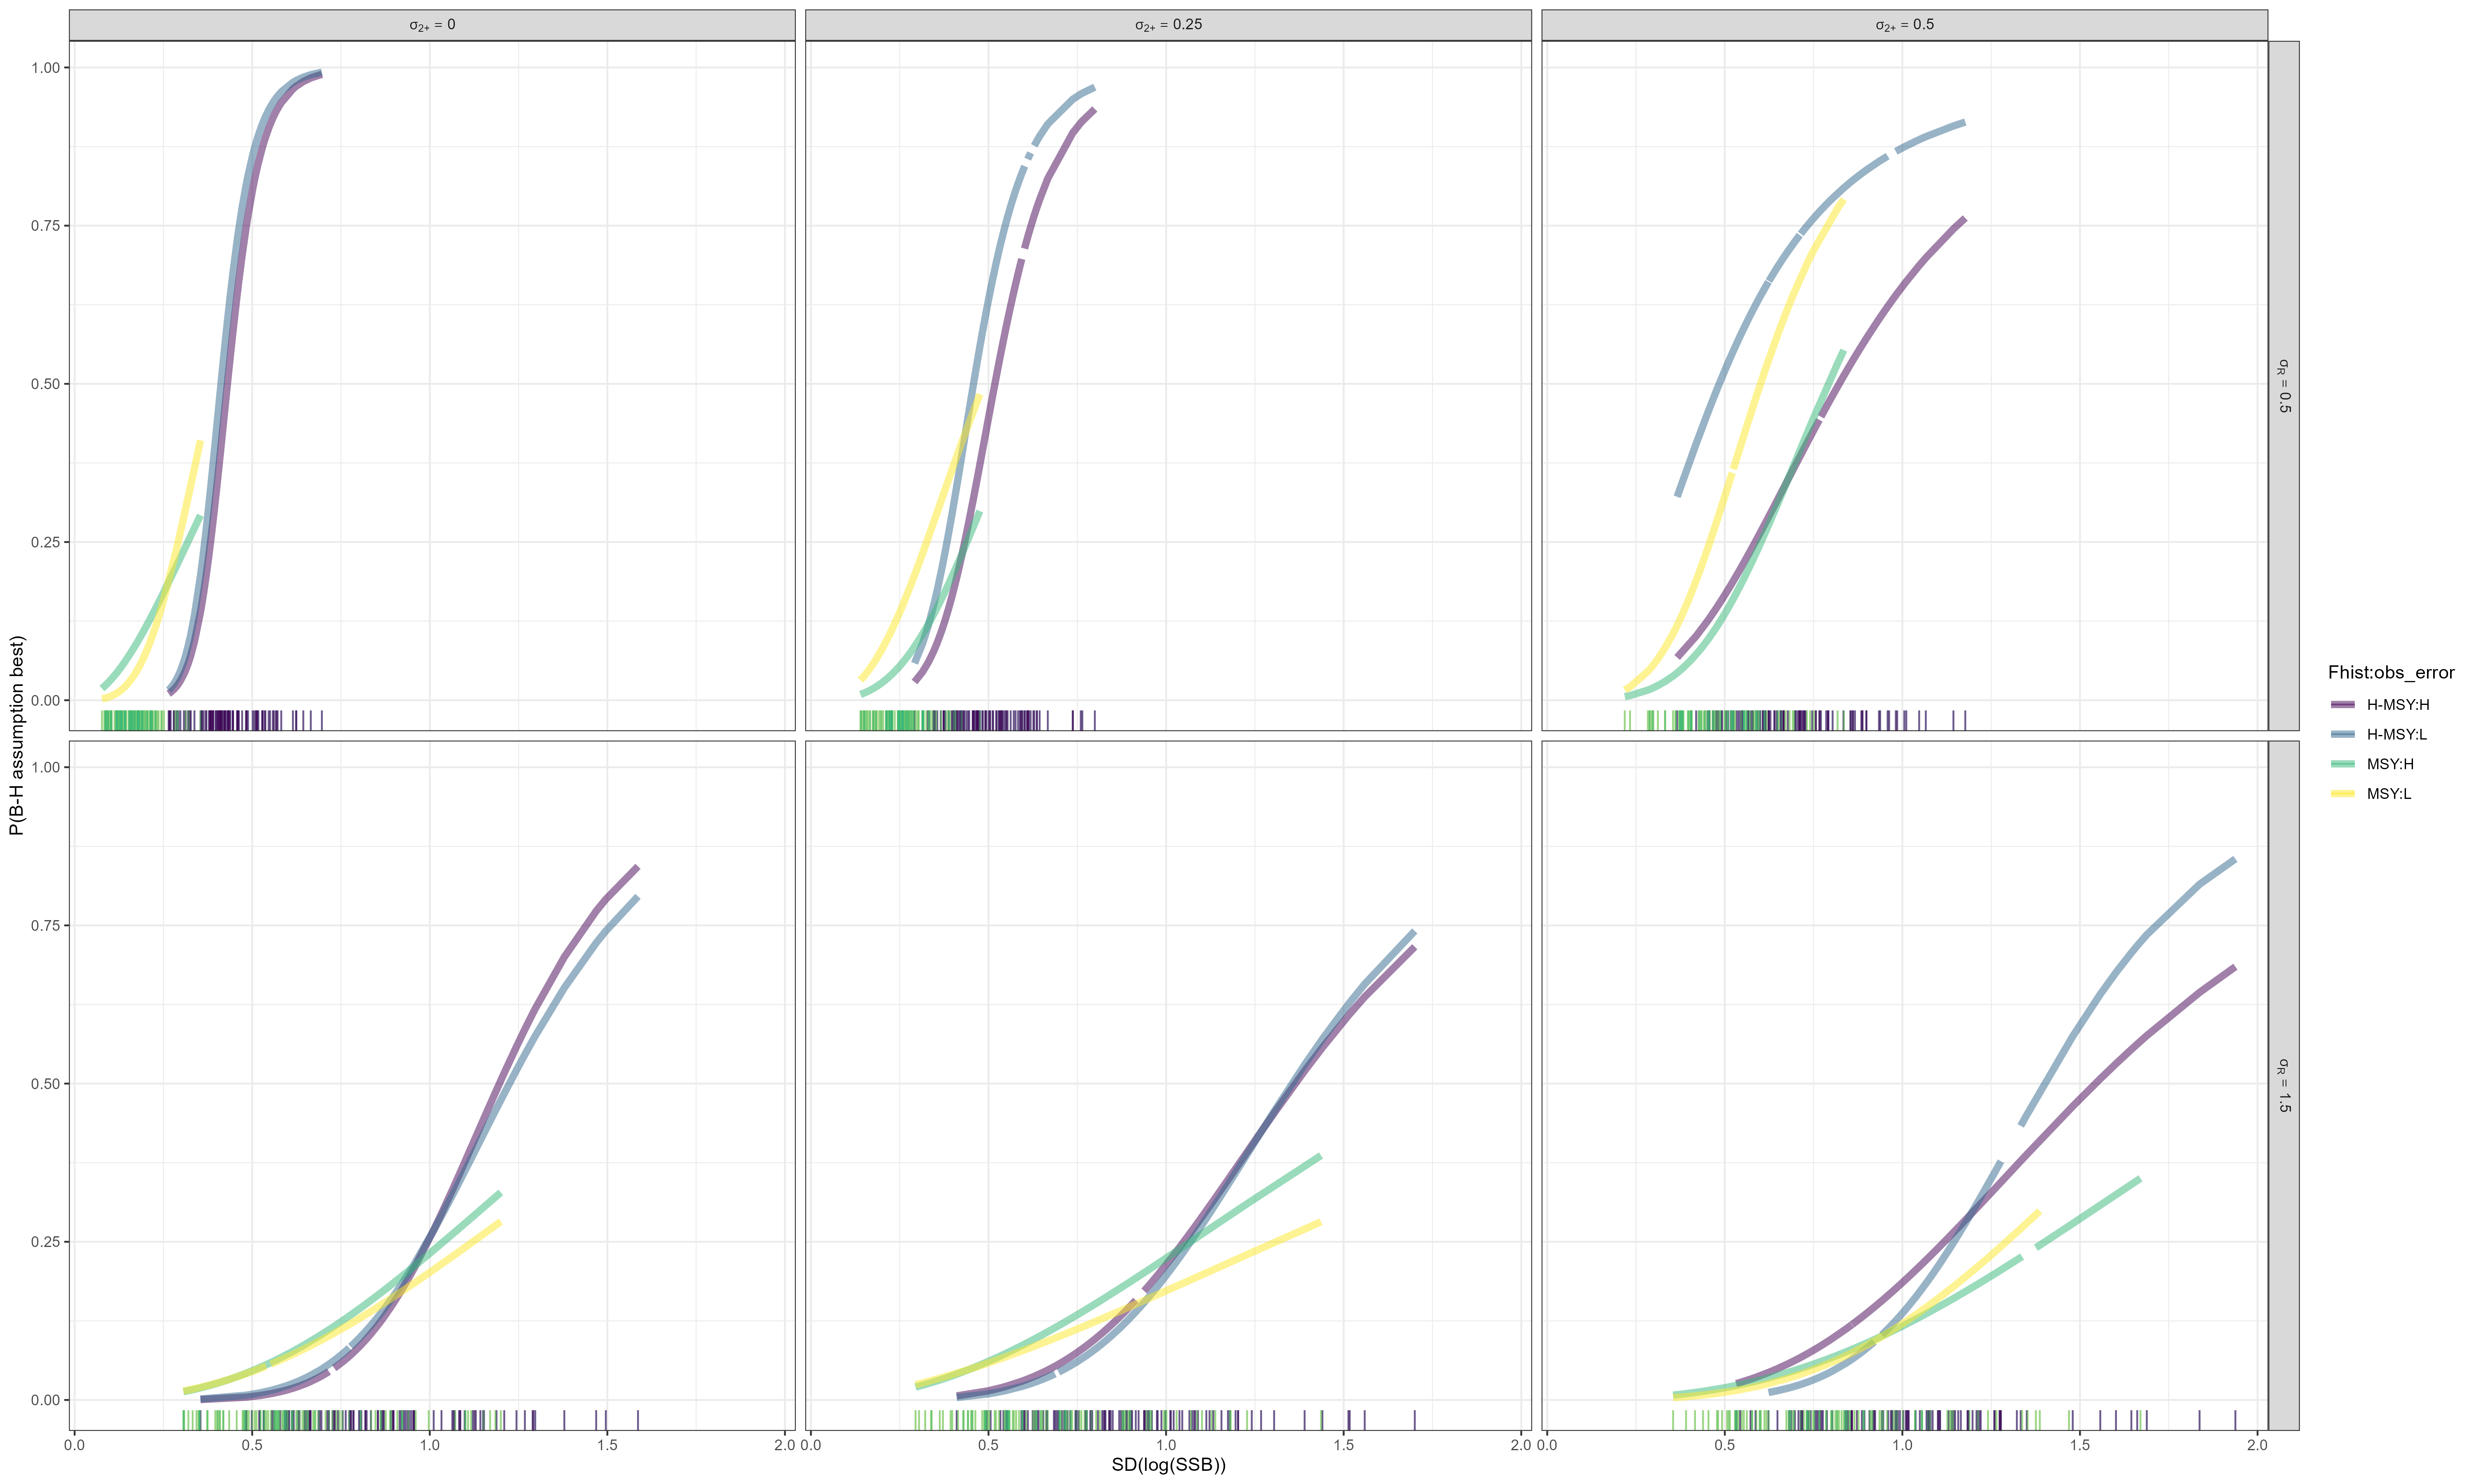
\includegraphics[width = \textwidth]{naa_om_MF_pred_BH_best.png}
\end{center}
\end{figure}

\begin{figure}
\caption{Predicted probability of AIC preferring BH model as a function of the variation of population SSB. Estimating models allow estimation of mean M.}\label{naa_om_ME_BH_glm_AIC_plots}
\begin{center}
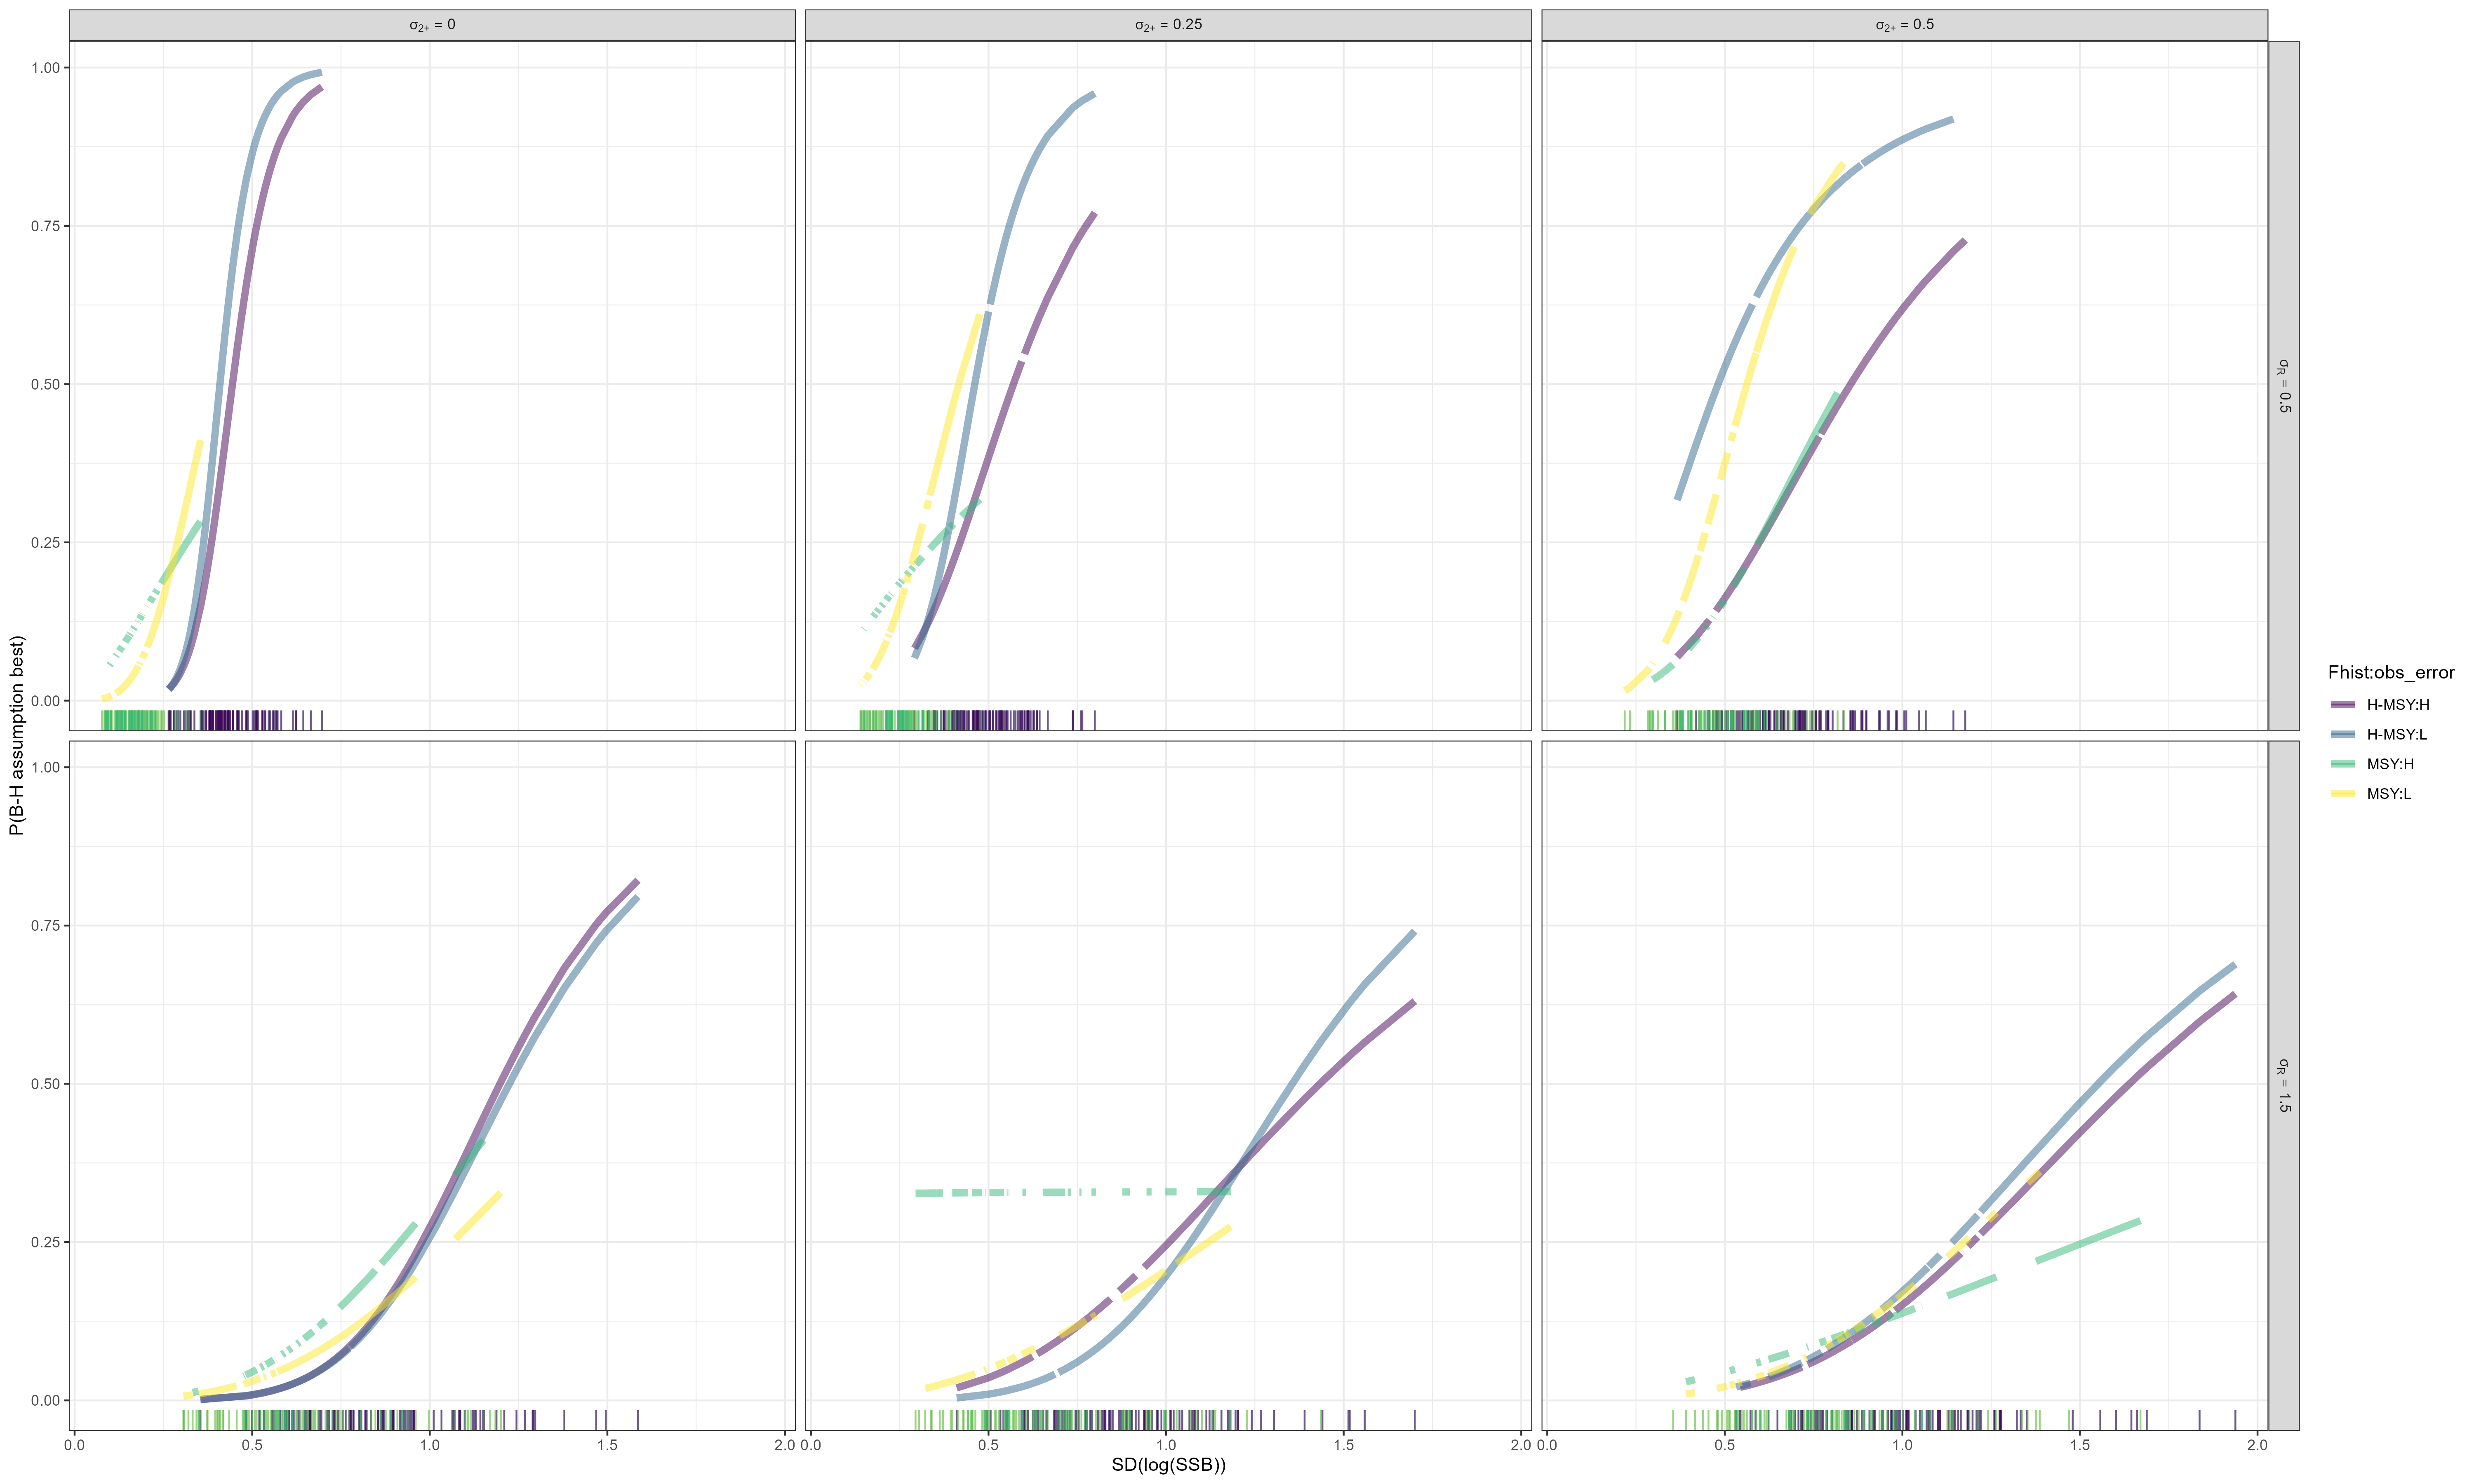
\includegraphics[width = \textwidth]{naa_om_ME_pred_BH_best.png}
\end{center}
\end{figure}

\hypertarget{rm-operating-models-2}{%
\subsubsection*{R+M operating models}\label{rm-operating-models-2}}
\addcontentsline{toc}{subsubsection}{R+M operating models}

\begin{table}
\caption{Operating models and estimation models all assume matching R+M process error structure, estimating models assume mean recruitment or a B-H stock recruit relationship and M is either fixed at the true value or estimated.}
{%latex.default(out, file = here("Project_0", "paper", "M_om_em_R_BH_aic_table.tex"),     table.env = FALSE, col.just = rep("r", dim(out)[2]), rowname = NULL)%
\begin{center}
\begin{tabular}{rrrrrrrr}
\hline\hline
\multicolumn{1}{c}{$\sigma_M$}&\multicolumn{1}{c}{$\rho_M$}&\multicolumn{1}{c}{F-history}&\multicolumn{1}{c}{Obs Error}&\multicolumn{1}{c}{R (M fix)}&\multicolumn{1}{c}{BH (M fix)}&\multicolumn{1}{c}{R (M est)}&\multicolumn{1}{c}{BH (M est)}\tabularnewline
\hline
$0.1$&$0.0$&H-MSY&L&$38$&$62$&$38$&$62$\tabularnewline
$0.5$&$0.0$&H-MSY&L&$42$&$58$&$42$&$58$\tabularnewline
$0.1$&$0.0$&MSY&L&$66$&$34$&$66$&$34$\tabularnewline
$0.5$&$0.0$&MSY&L&$70$&$30$&$58$&$41$\tabularnewline
$0.1$&$0.0$&H-MSY&H&$45$&$55$&$47$&$53$\tabularnewline
$0.5$&$0.0$&H-MSY&H&$56$&$43$&$54$&$45$\tabularnewline
$0.1$&$0.0$&MSY&H&$66$&$34$&$66$&$33$\tabularnewline
$0.5$&$0.0$&MSY&H&$72$&$28$&$57$&$42$\tabularnewline
$0.1$&$0.9$&H-MSY&L&$31$&$69$&$33$&$64$\tabularnewline
$0.5$&$0.9$&H-MSY&L&$15$&$73$&$16$&$64$\tabularnewline
$0.1$&$0.9$&MSY&L&$44$&$56$&$41$&$47$\tabularnewline
$0.5$&$0.9$&MSY&L&$12$&$76$&$10$&$69$\tabularnewline
$0.1$&$0.9$&H-MSY&H&$32$&$68$&$47$&$44$\tabularnewline
$0.5$&$0.9$&H-MSY&H&$10$&$78$&$21$&$51$\tabularnewline
$0.1$&$0.9$&MSY&H&$40$&$60$&$38$&$28$\tabularnewline
$0.5$&$0.9$&MSY&H&$22$&$64$&$22$&$49$\tabularnewline
\hline
\end{tabular}\end{center}
}
\end{table}

\begin{figure}
\caption{Predicted probability of AIC preferring BH model as a function of the variation of population SSB. Operating and estimating models have matching R+M process error structures. Estimating models assume mean M is fixed at the true value.}\label{M_om_MF_BH_glm_AIC_plots}
\begin{center}
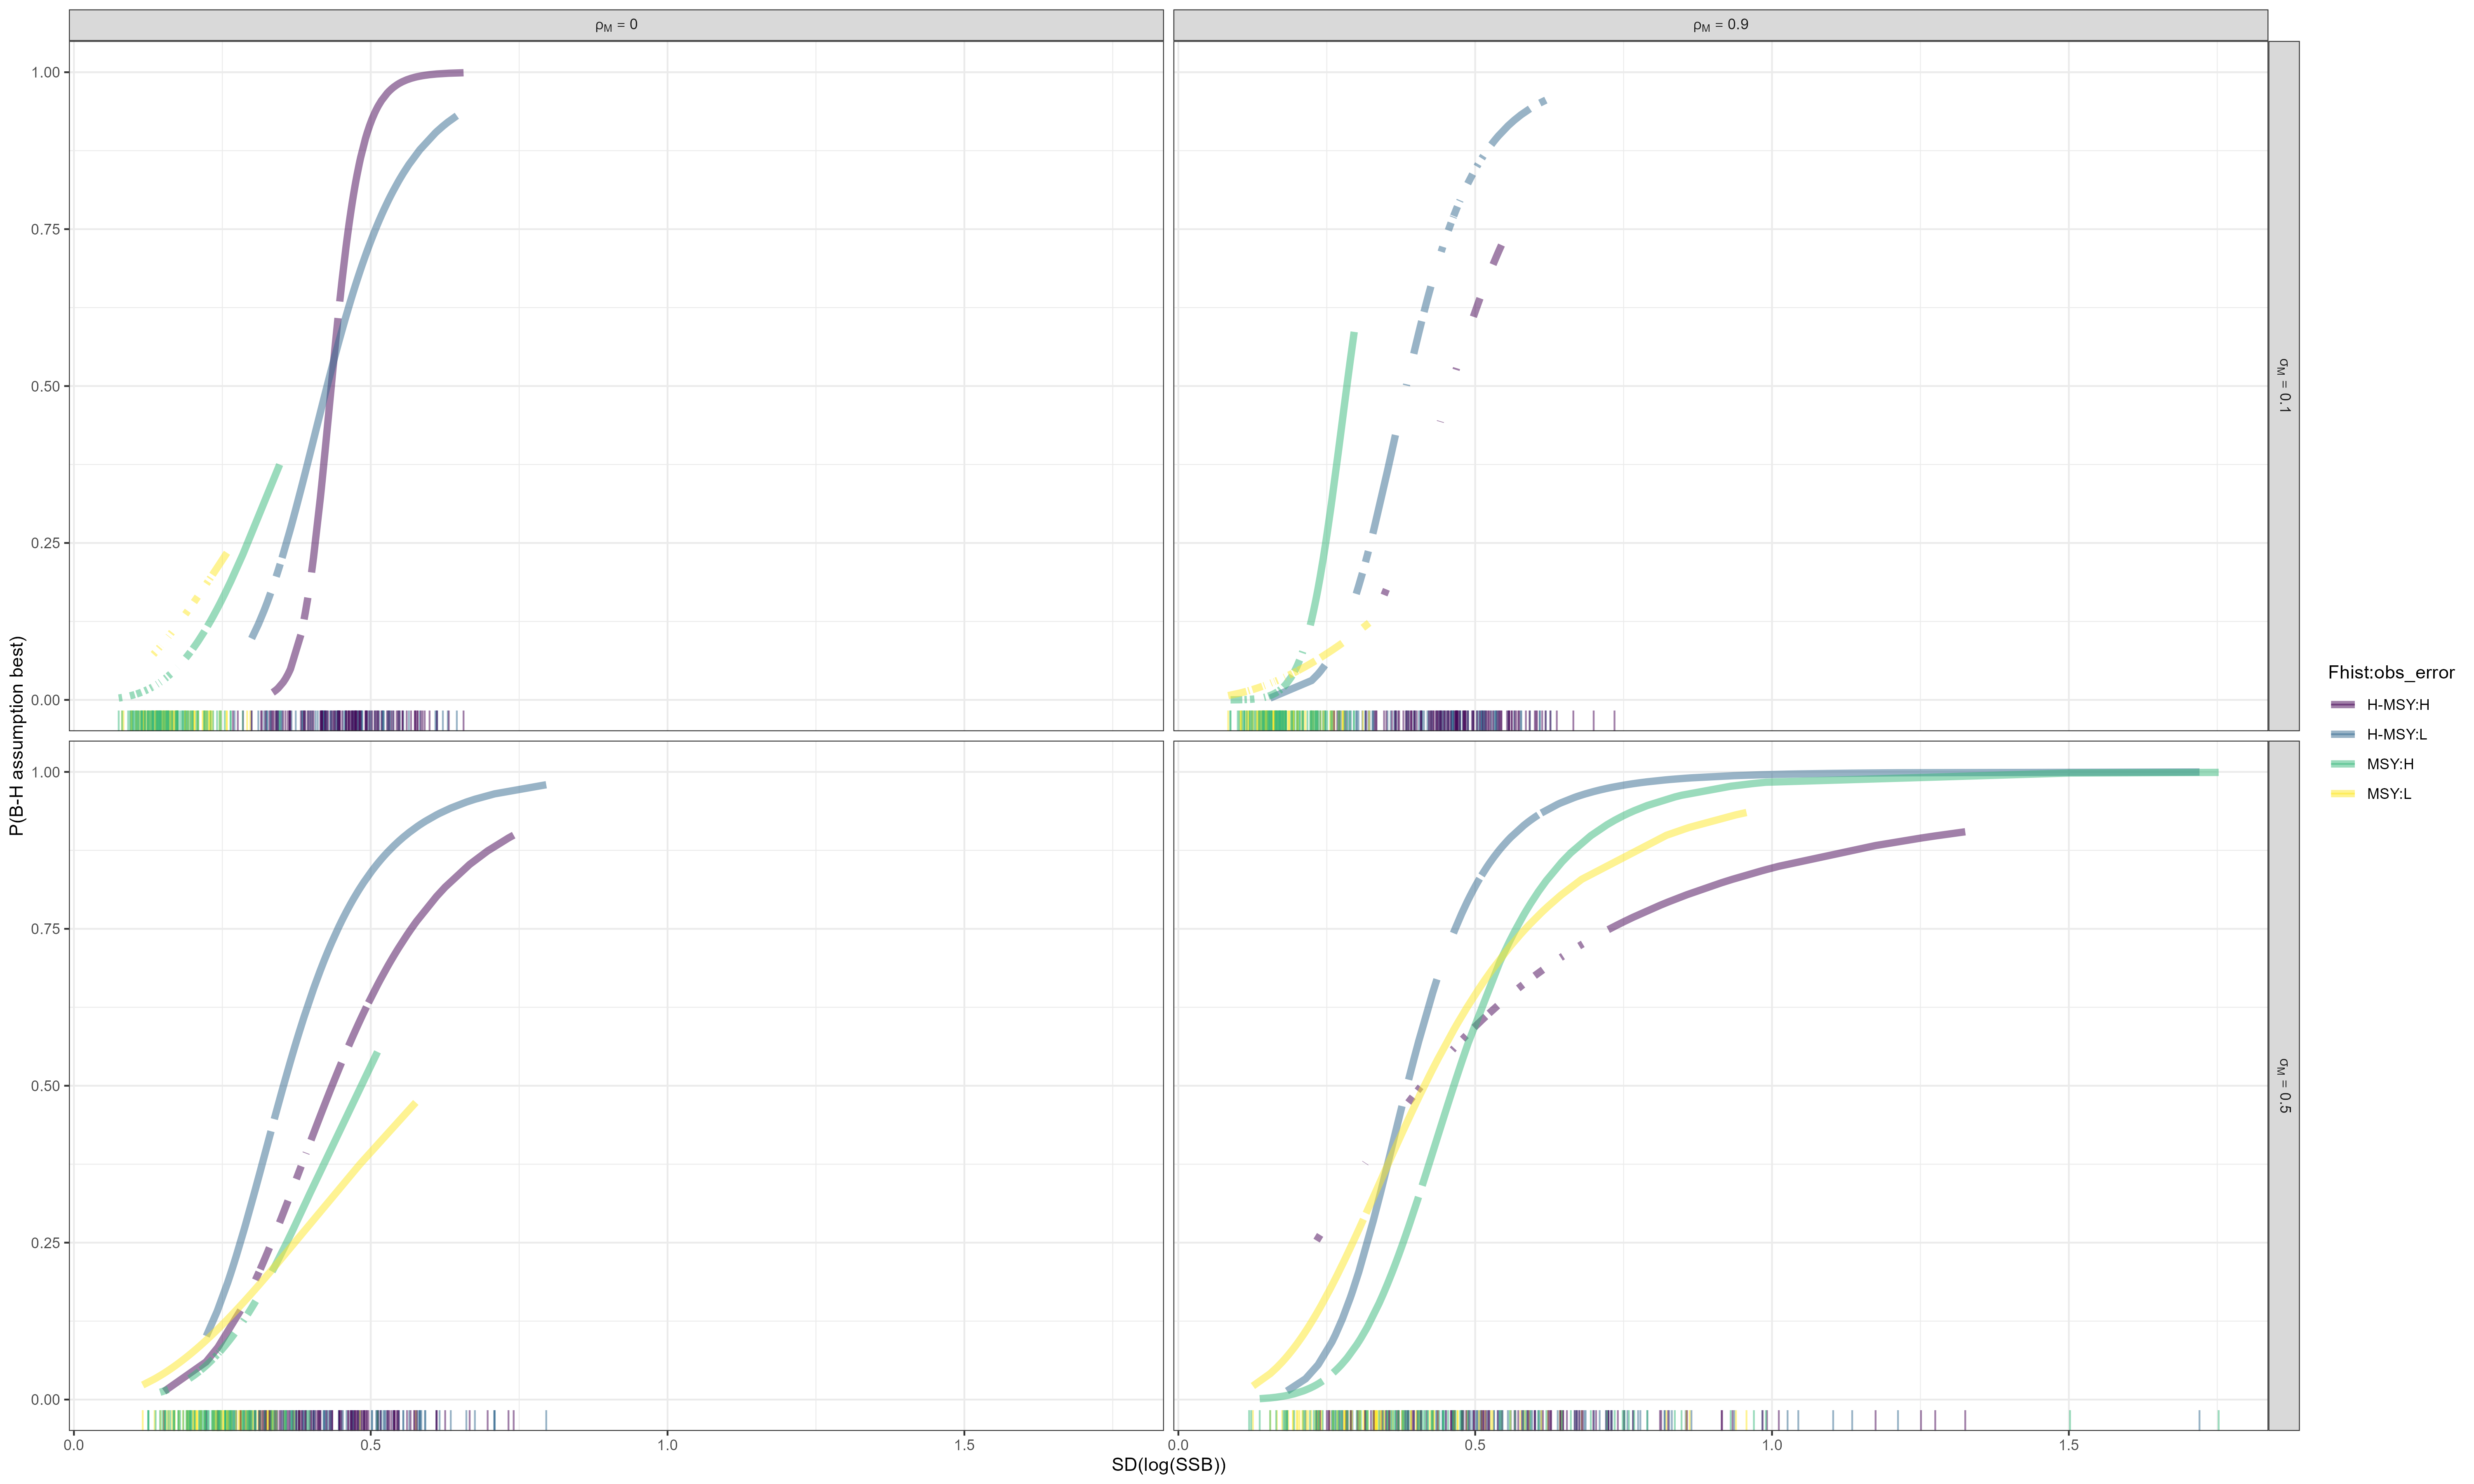
\includegraphics[width = \textwidth]{M_om_MF_pred_BH_best.png}
\end{center}
\end{figure}

\begin{figure}
\caption{Predicted probability of AIC preferring BH model as a function of the variation of population SSB. Operating and estimating models have matching R+M process error structures. Estimating models allow estimation of mean M.}\label{M_om_ME_BH_glm_AIC_plots}
\begin{center}
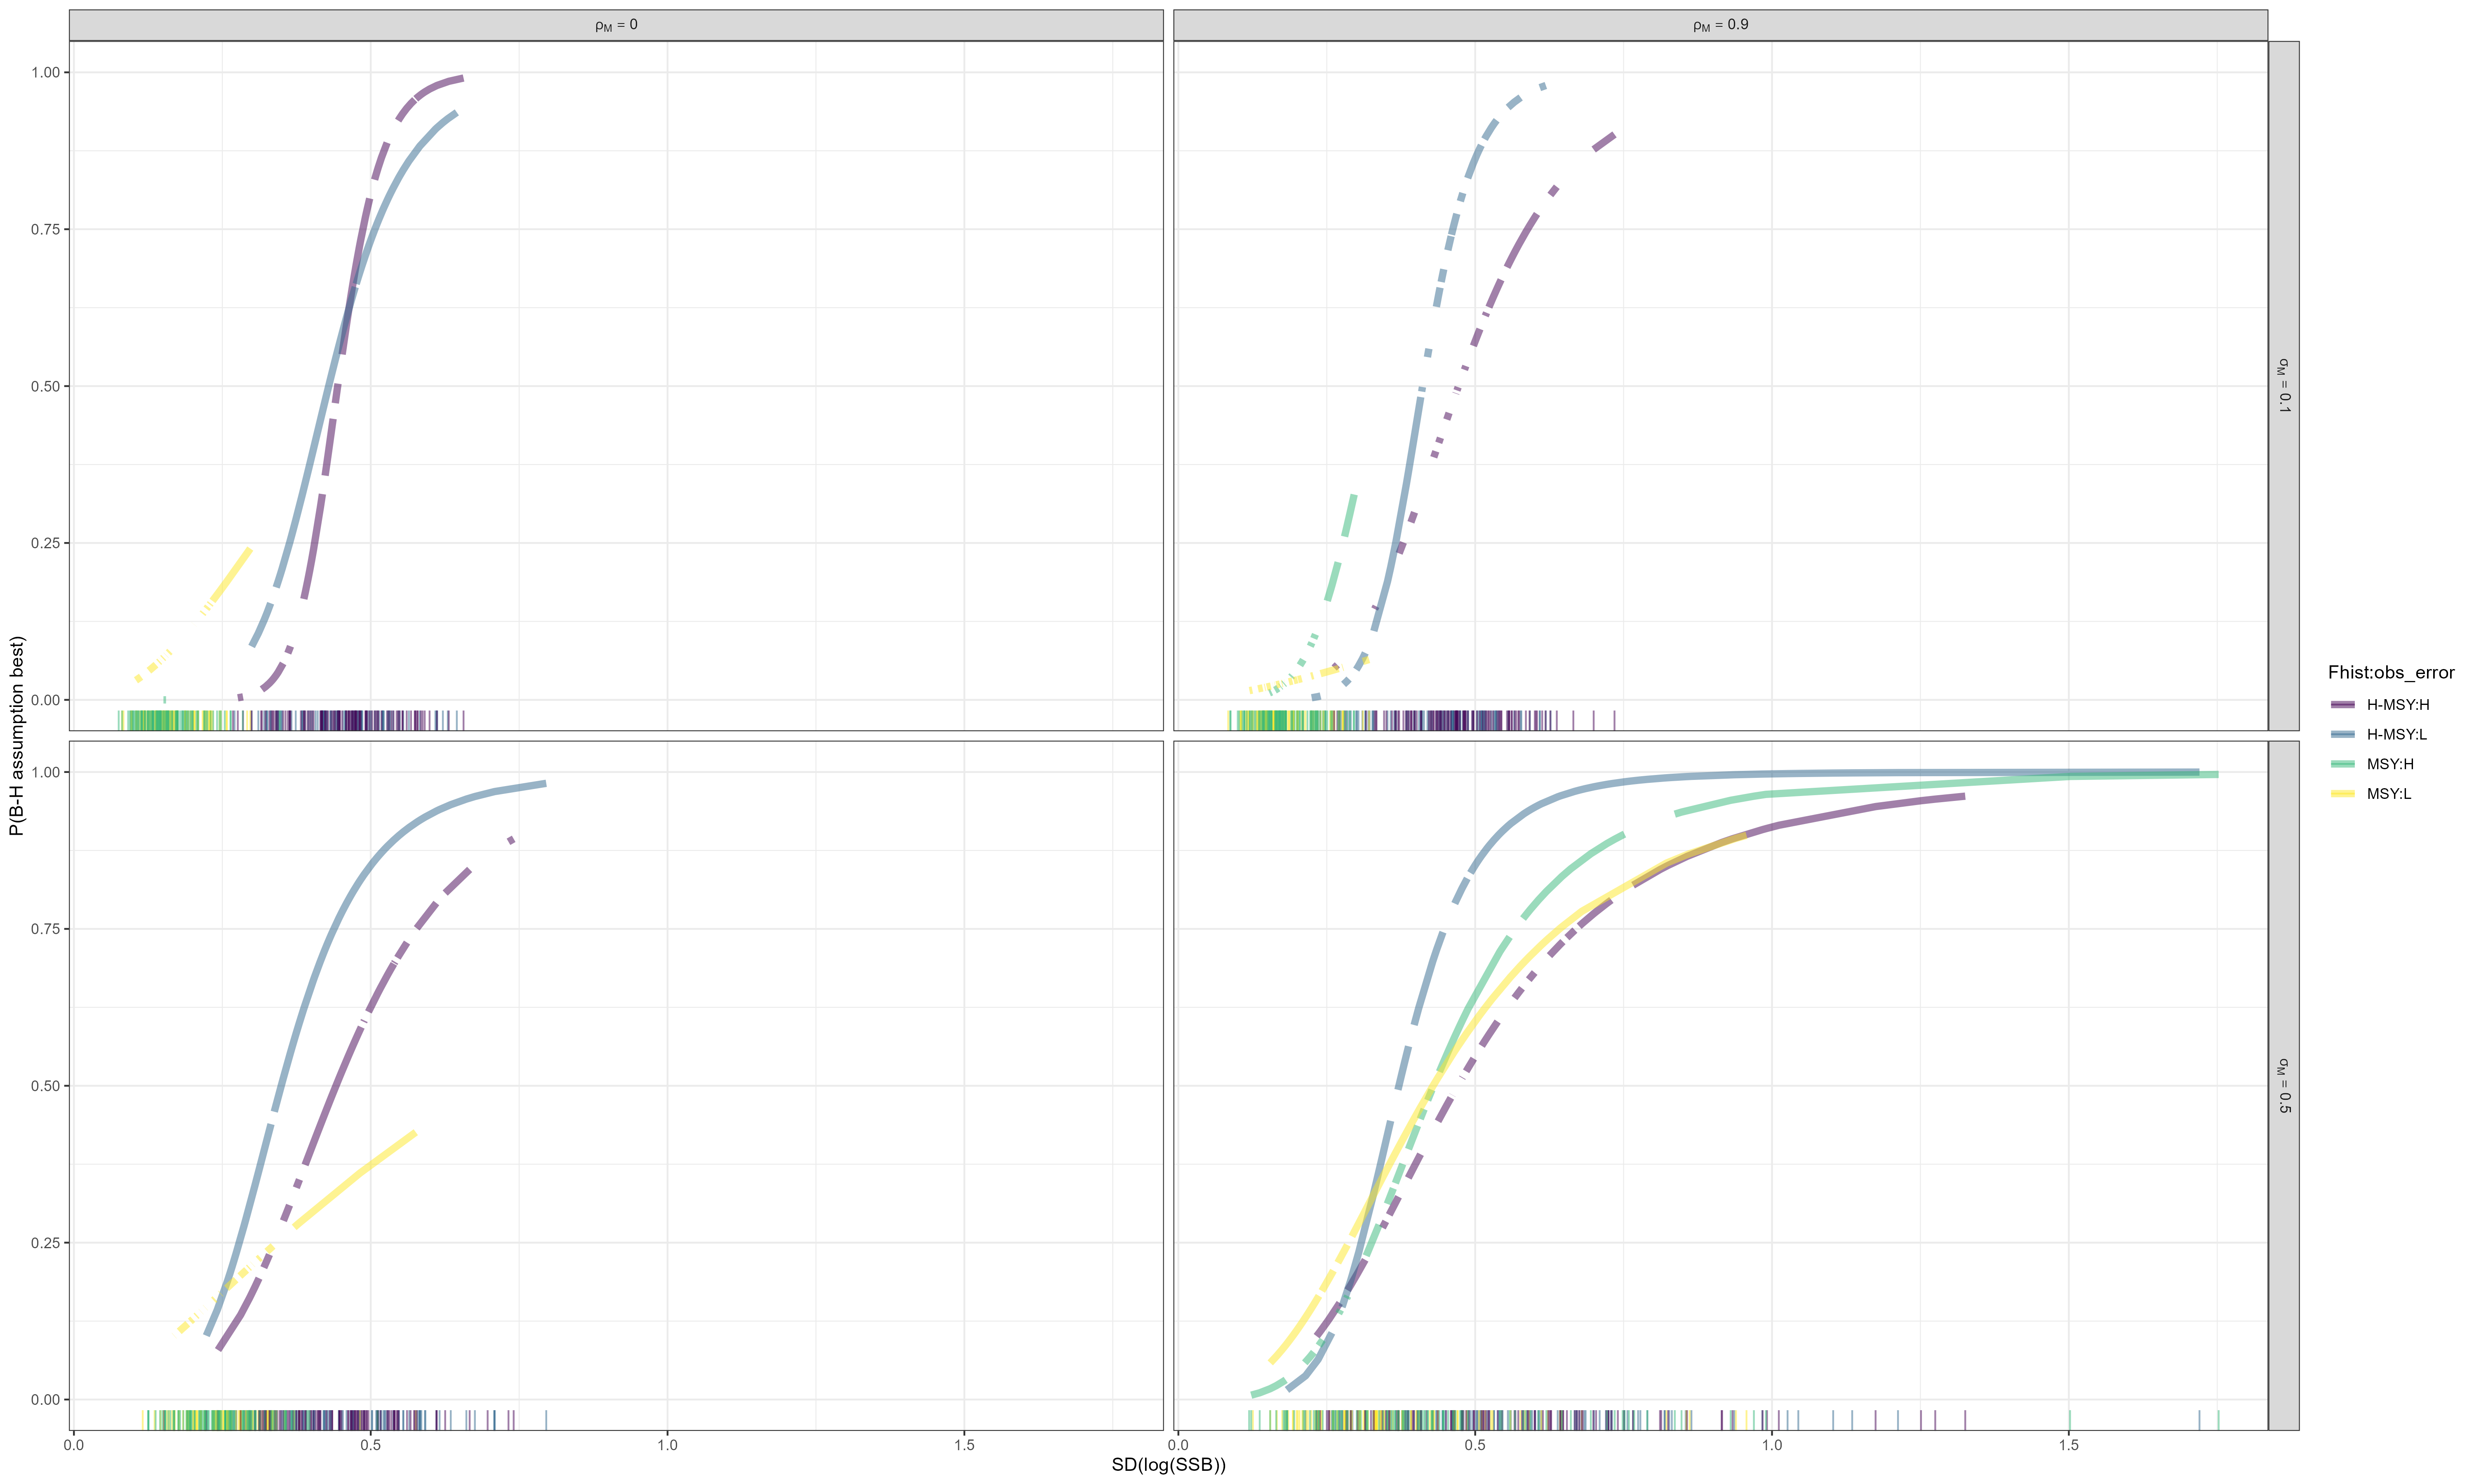
\includegraphics[width = \textwidth]{M_om_ME_pred_BH_best.png}
\end{center}
\end{figure}

\hypertarget{rsel-operating-models-2}{%
\subsubsection*{R+Sel operating models}\label{rsel-operating-models-2}}
\addcontentsline{toc}{subsubsection}{R+Sel operating models}

\begin{table}
\caption{Operating models and estimation models all assume matching R+Sel process error structure, estimating models assume mean recruitment or a B-H stock recruit relationship and M is either fixed at the true value or estimated.}
{\begin{center}
\begin{tabular}{rrrrrrrr}
\hline\hline
\multicolumn{1}{c}{$\sigma_{Sel}$}&\multicolumn{1}{c}{$\rho_{Sel}$}&\multicolumn{1}{c}{F-history}&\multicolumn{1}{c}{Obs Error}&\multicolumn{1}{c}{R (M fix)}&\multicolumn{1}{c}{BH (M fix)}&\multicolumn{1}{c}{R (M est)}&\multicolumn{1}{c}{BH (M est)}\tabularnewline
\hline
$0.1$&$0.0$&H-MSY&L&$40$&$60$&$40$&$60$\tabularnewline
$0.5$&$0.0$&H-MSY&L&$27$&$73$&$25$&$75$\tabularnewline
$0.1$&$0.0$&MSY&L&$94$&$ 6$&$95$&$ 5$\tabularnewline
$0.5$&$0.0$&MSY&L&$95$&$ 5$&$94$&$ 6$\tabularnewline
$0.1$&$0.0$&H-MSY&H&$51$&$49$&$55$&$44$\tabularnewline
$0.5$&$0.0$&H-MSY&H&$41$&$59$&$41$&$58$\tabularnewline
$0.1$&$0.0$&MSY&H&$95$&$ 5$&$77$&$11$\tabularnewline
$0.5$&$0.0$&MSY&H&$95$&$ 5$&$94$&$ 6$\tabularnewline
$0.1$&$0.9$&H-MSY&L&$50$&$50$&$48$&$52$\tabularnewline
$0.5$&$0.9$&H-MSY&L&$42$&$58$&$45$&$55$\tabularnewline
$0.1$&$0.9$&MSY&L&$92$&$ 8$&$94$&$ 6$\tabularnewline
$0.5$&$0.9$&MSY&L&$94$&$ 6$&$94$&$ 6$\tabularnewline
$0.1$&$0.9$&H-MSY&H&$48$&$52$&$52$&$48$\tabularnewline
$0.5$&$0.9$&H-MSY&H&$53$&$47$&$54$&$46$\tabularnewline
$0.1$&$0.9$&MSY&H&$97$&$ 3$&$80$&$ 9$\tabularnewline
$0.5$&$0.9$&MSY&H&$96$&$ 4$&$95$&$ 3$\tabularnewline
\hline
\end{tabular}\end{center}
}
\end{table}

\begin{figure}
\caption{Predicted probability of AIC preferring BH model as a function of the variation of population SSB. Operating and estimating models have matching R+Sel process error structures. Estimating models assume mean M is fixed at the true value.}\label{Sel_om_MF_BH_glm_AIC_plots}
\begin{center}
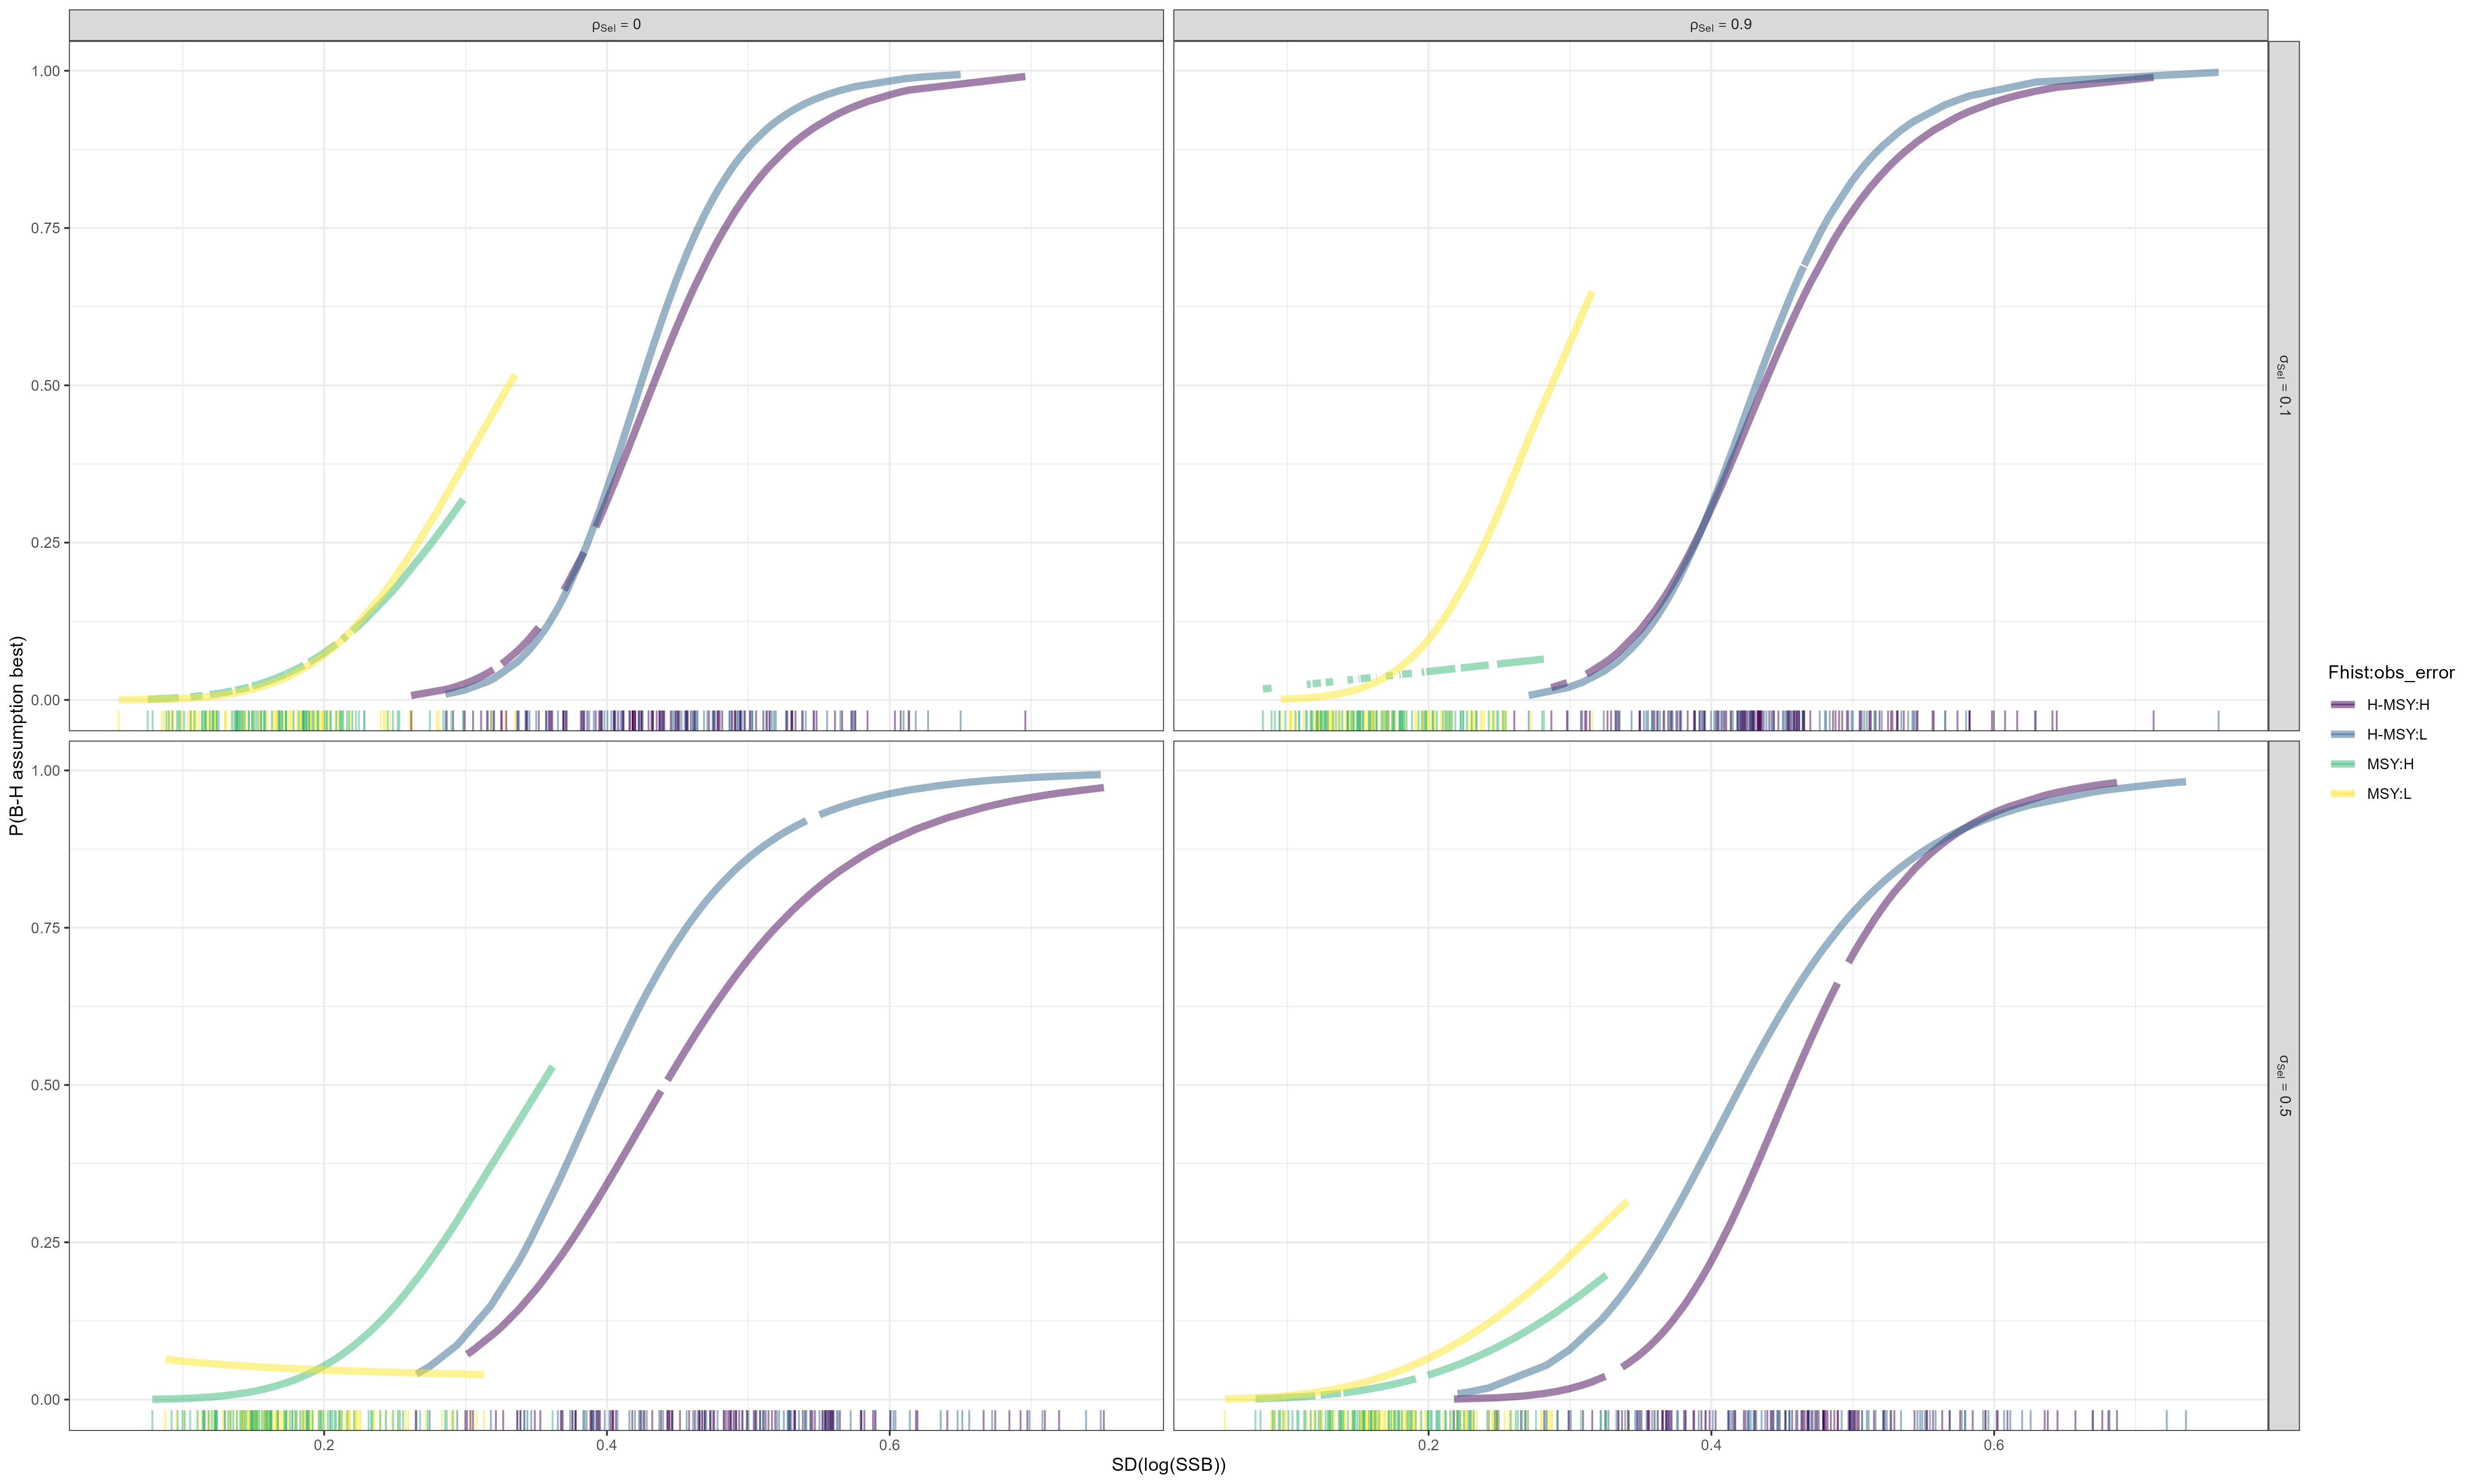
\includegraphics[width = \textwidth]{Sel_om_MF_pred_BH_best.png}
\end{center}
\end{figure}

\begin{figure}
\caption{Predicted probability of AIC preferring BH model as a function of the variation of population SSB. Operating and estimating models have matching R+Sel process error structures. Estimating models allow estimation of mean M.}\label{Sel_om_ME_BH_glm_AIC_plots}
\begin{center}
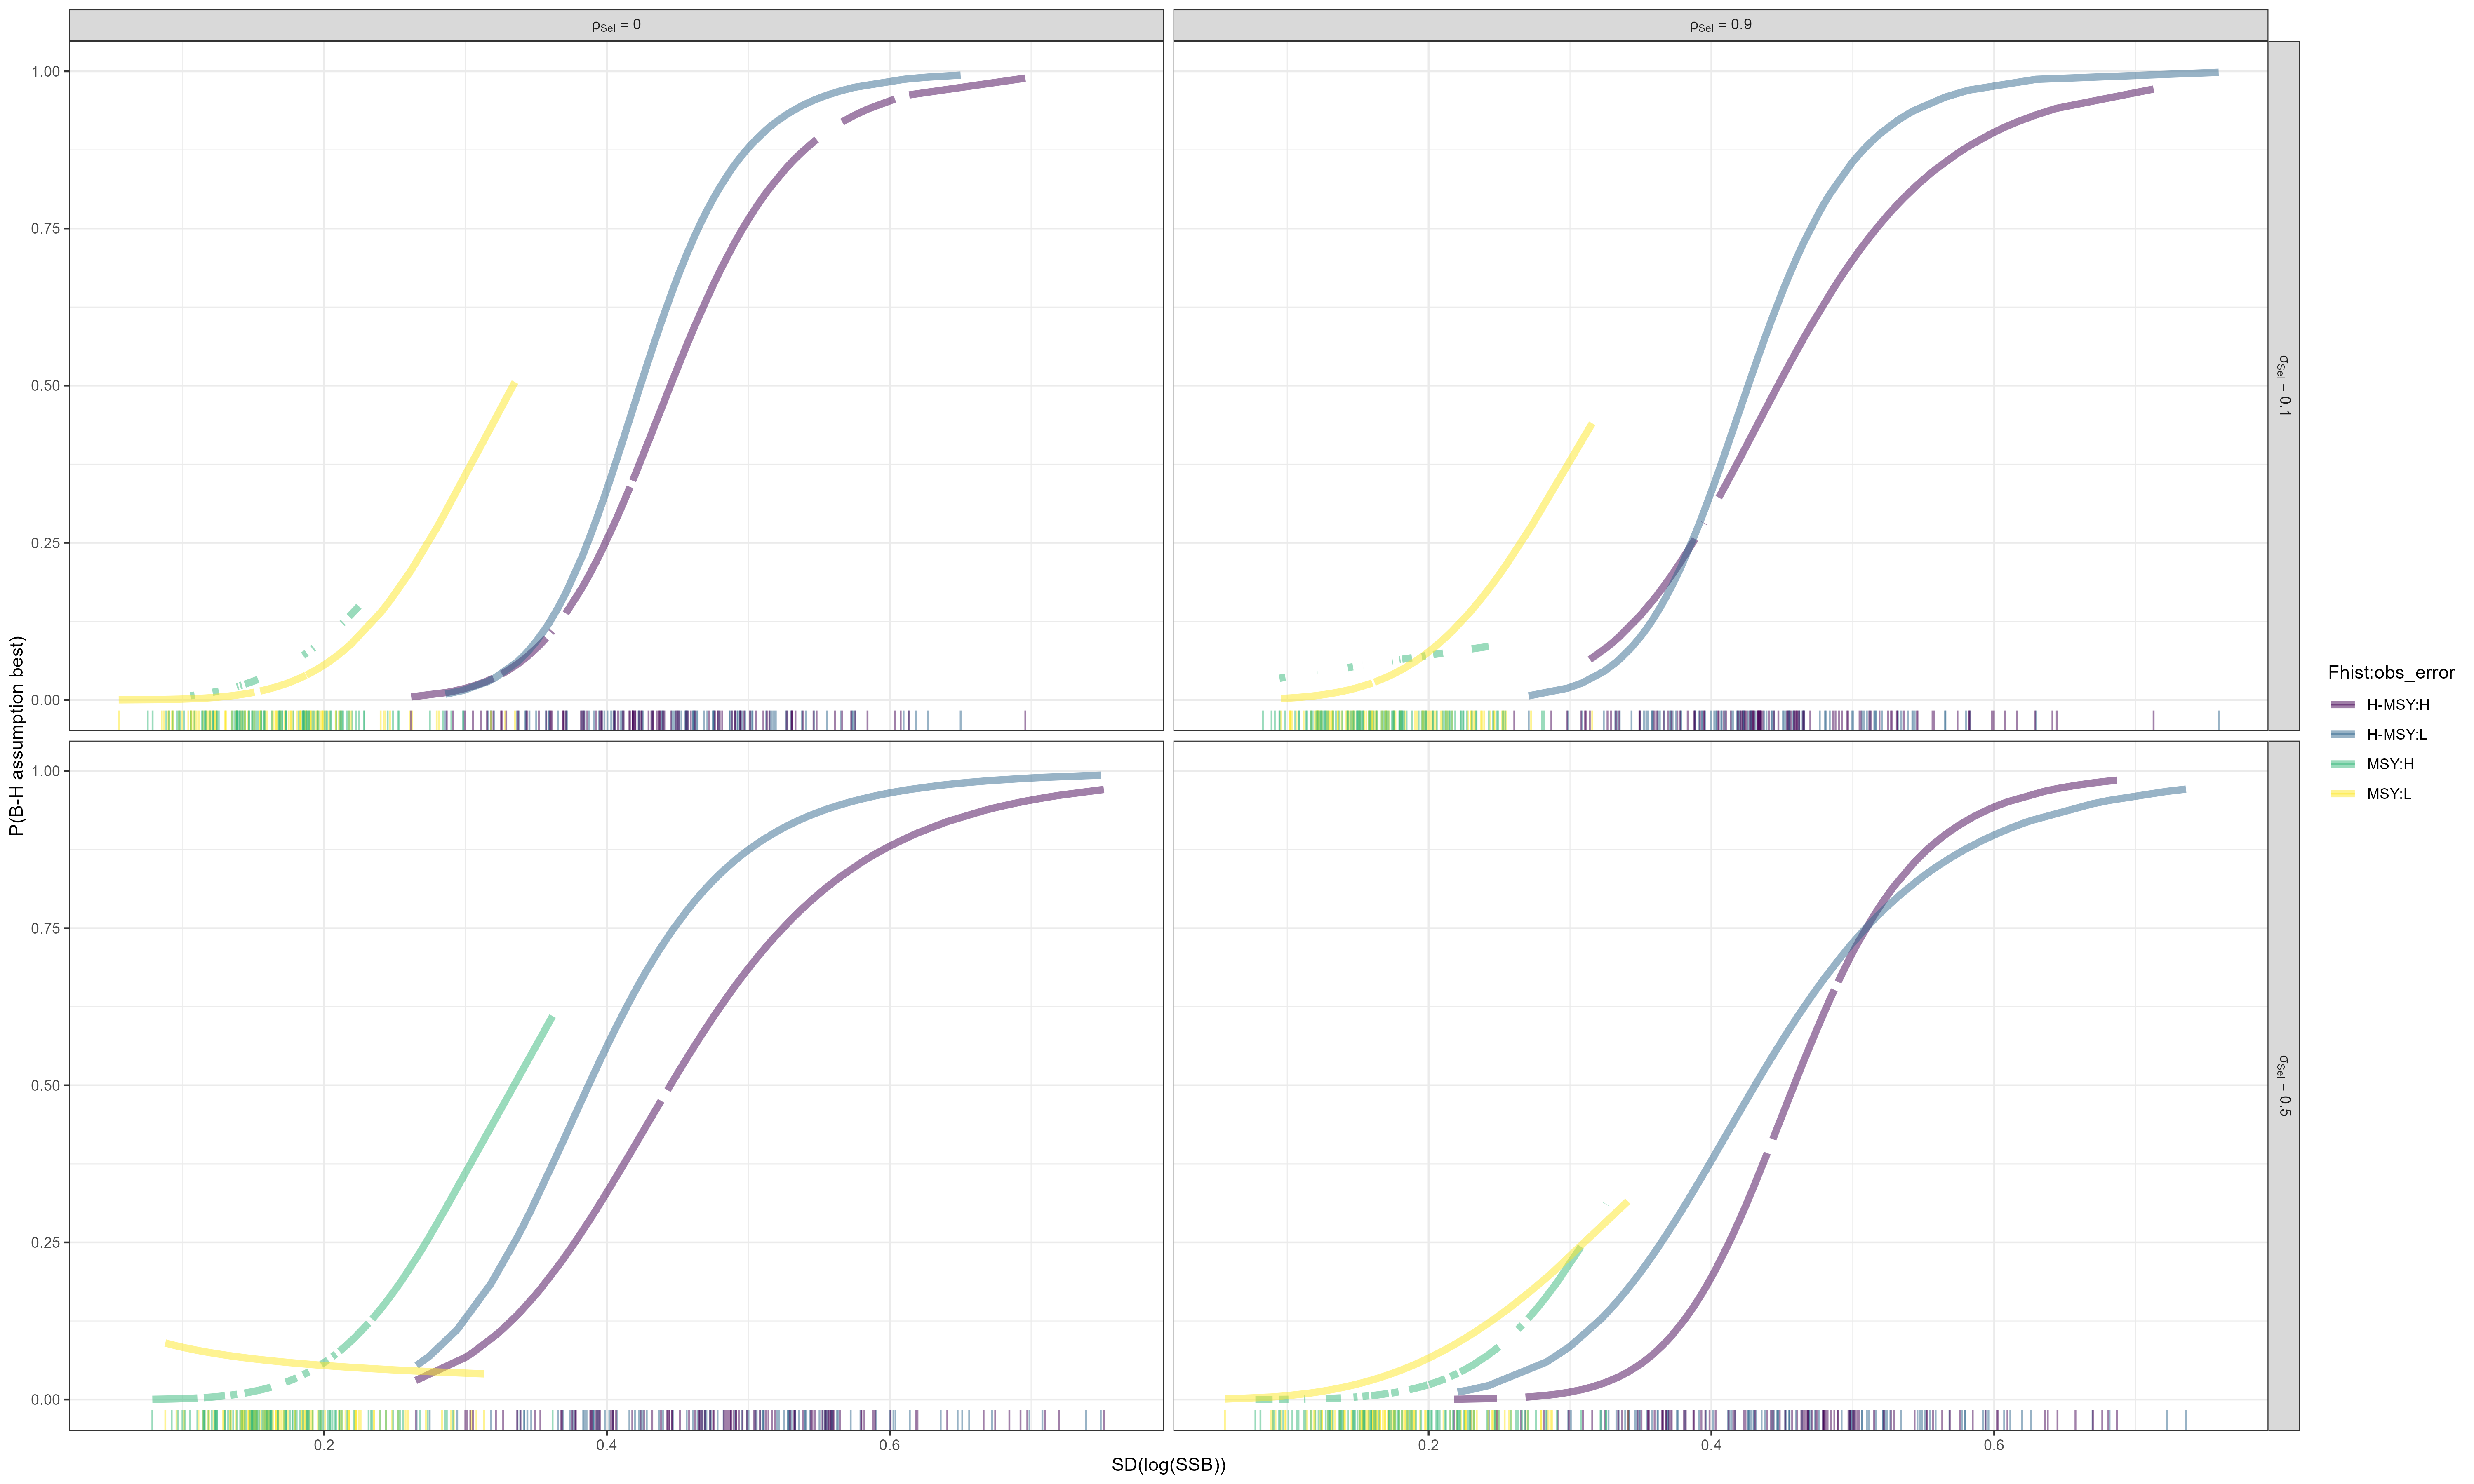
\includegraphics[width = \textwidth]{Sel_om_ME_pred_BH_best.png}
\end{center}
\end{figure}

\hypertarget{rq-operating-models-2}{%
\subsubsection*{R+q operating models}\label{rq-operating-models-2}}
\addcontentsline{toc}{subsubsection}{R+q operating models}

\begin{table}
\caption{Operating models and estimation models all assume matching R+q process error structure, estimating models assume mean recruitment or a B-H stock recruit relationship and M is either fixed at the true value or estimated.}
{\begin{center}
\begin{tabular}{rrrrrrrr}
\hline\hline
\multicolumn{1}{c}{$\sigma_{q}$}&\multicolumn{1}{c}{$\rho_{q}$}&\multicolumn{1}{c}{F-history}&\multicolumn{1}{c}{Obs Error}&\multicolumn{1}{c}{R (M fix)}&\multicolumn{1}{c}{BH (M fix)}&\multicolumn{1}{c}{R (M est)}&\multicolumn{1}{c}{BH (M est)}\tabularnewline
\hline
$0.1$&$0.0$&H-MSY&L&$39$&$61$&$41$&$59$\tabularnewline
$0.5$&$0.0$&H-MSY&L&$46$&$54$&$45$&$55$\tabularnewline
$0.1$&$0.0$&MSY&L&$95$&$ 5$&$95$&$ 5$\tabularnewline
$0.5$&$0.0$&MSY&L&$97$&$ 3$&$95$&$ 5$\tabularnewline
$0.1$&$0.0$&H-MSY&H&$47$&$53$&$52$&$48$\tabularnewline
$0.5$&$0.0$&H-MSY&H&$55$&$45$&$62$&$38$\tabularnewline
$0.1$&$0.0$&MSY&H&$92$&$ 8$&$49$&$ 6$\tabularnewline
$0.5$&$0.0$&MSY&H&$96$&$ 4$&$95$&$ 5$\tabularnewline
$0.1$&$0.9$&H-MSY&L&$38$&$62$&$40$&$60$\tabularnewline
$0.5$&$0.9$&H-MSY&L&$45$&$55$&$47$&$53$\tabularnewline
$0.1$&$0.9$&MSY&L&$96$&$ 4$&$94$&$ 5$\tabularnewline
$0.5$&$0.9$&MSY&L&$97$&$ 3$&$97$&$ 3$\tabularnewline
$0.1$&$0.9$&H-MSY&H&$51$&$49$&$56$&$44$\tabularnewline
$0.5$&$0.9$&H-MSY&H&$51$&$49$&$56$&$44$\tabularnewline
$0.1$&$0.9$&MSY&H&$98$&$ 2$&$81$&$ 6$\tabularnewline
$0.5$&$0.9$&MSY&H&$97$&$ 3$&$97$&$ 3$\tabularnewline
\hline
\end{tabular}\end{center}
}
\end{table}

\begin{figure}
\caption{Predicted probability of AIC preferring BH model as a function of the variation of population SSB. Operating and estimating models have matching R+q process error structures. Estimating models assume mean M is fixed at the true value.}\label{q_om_MF_BH_glm_AIC_plots}
\begin{center}
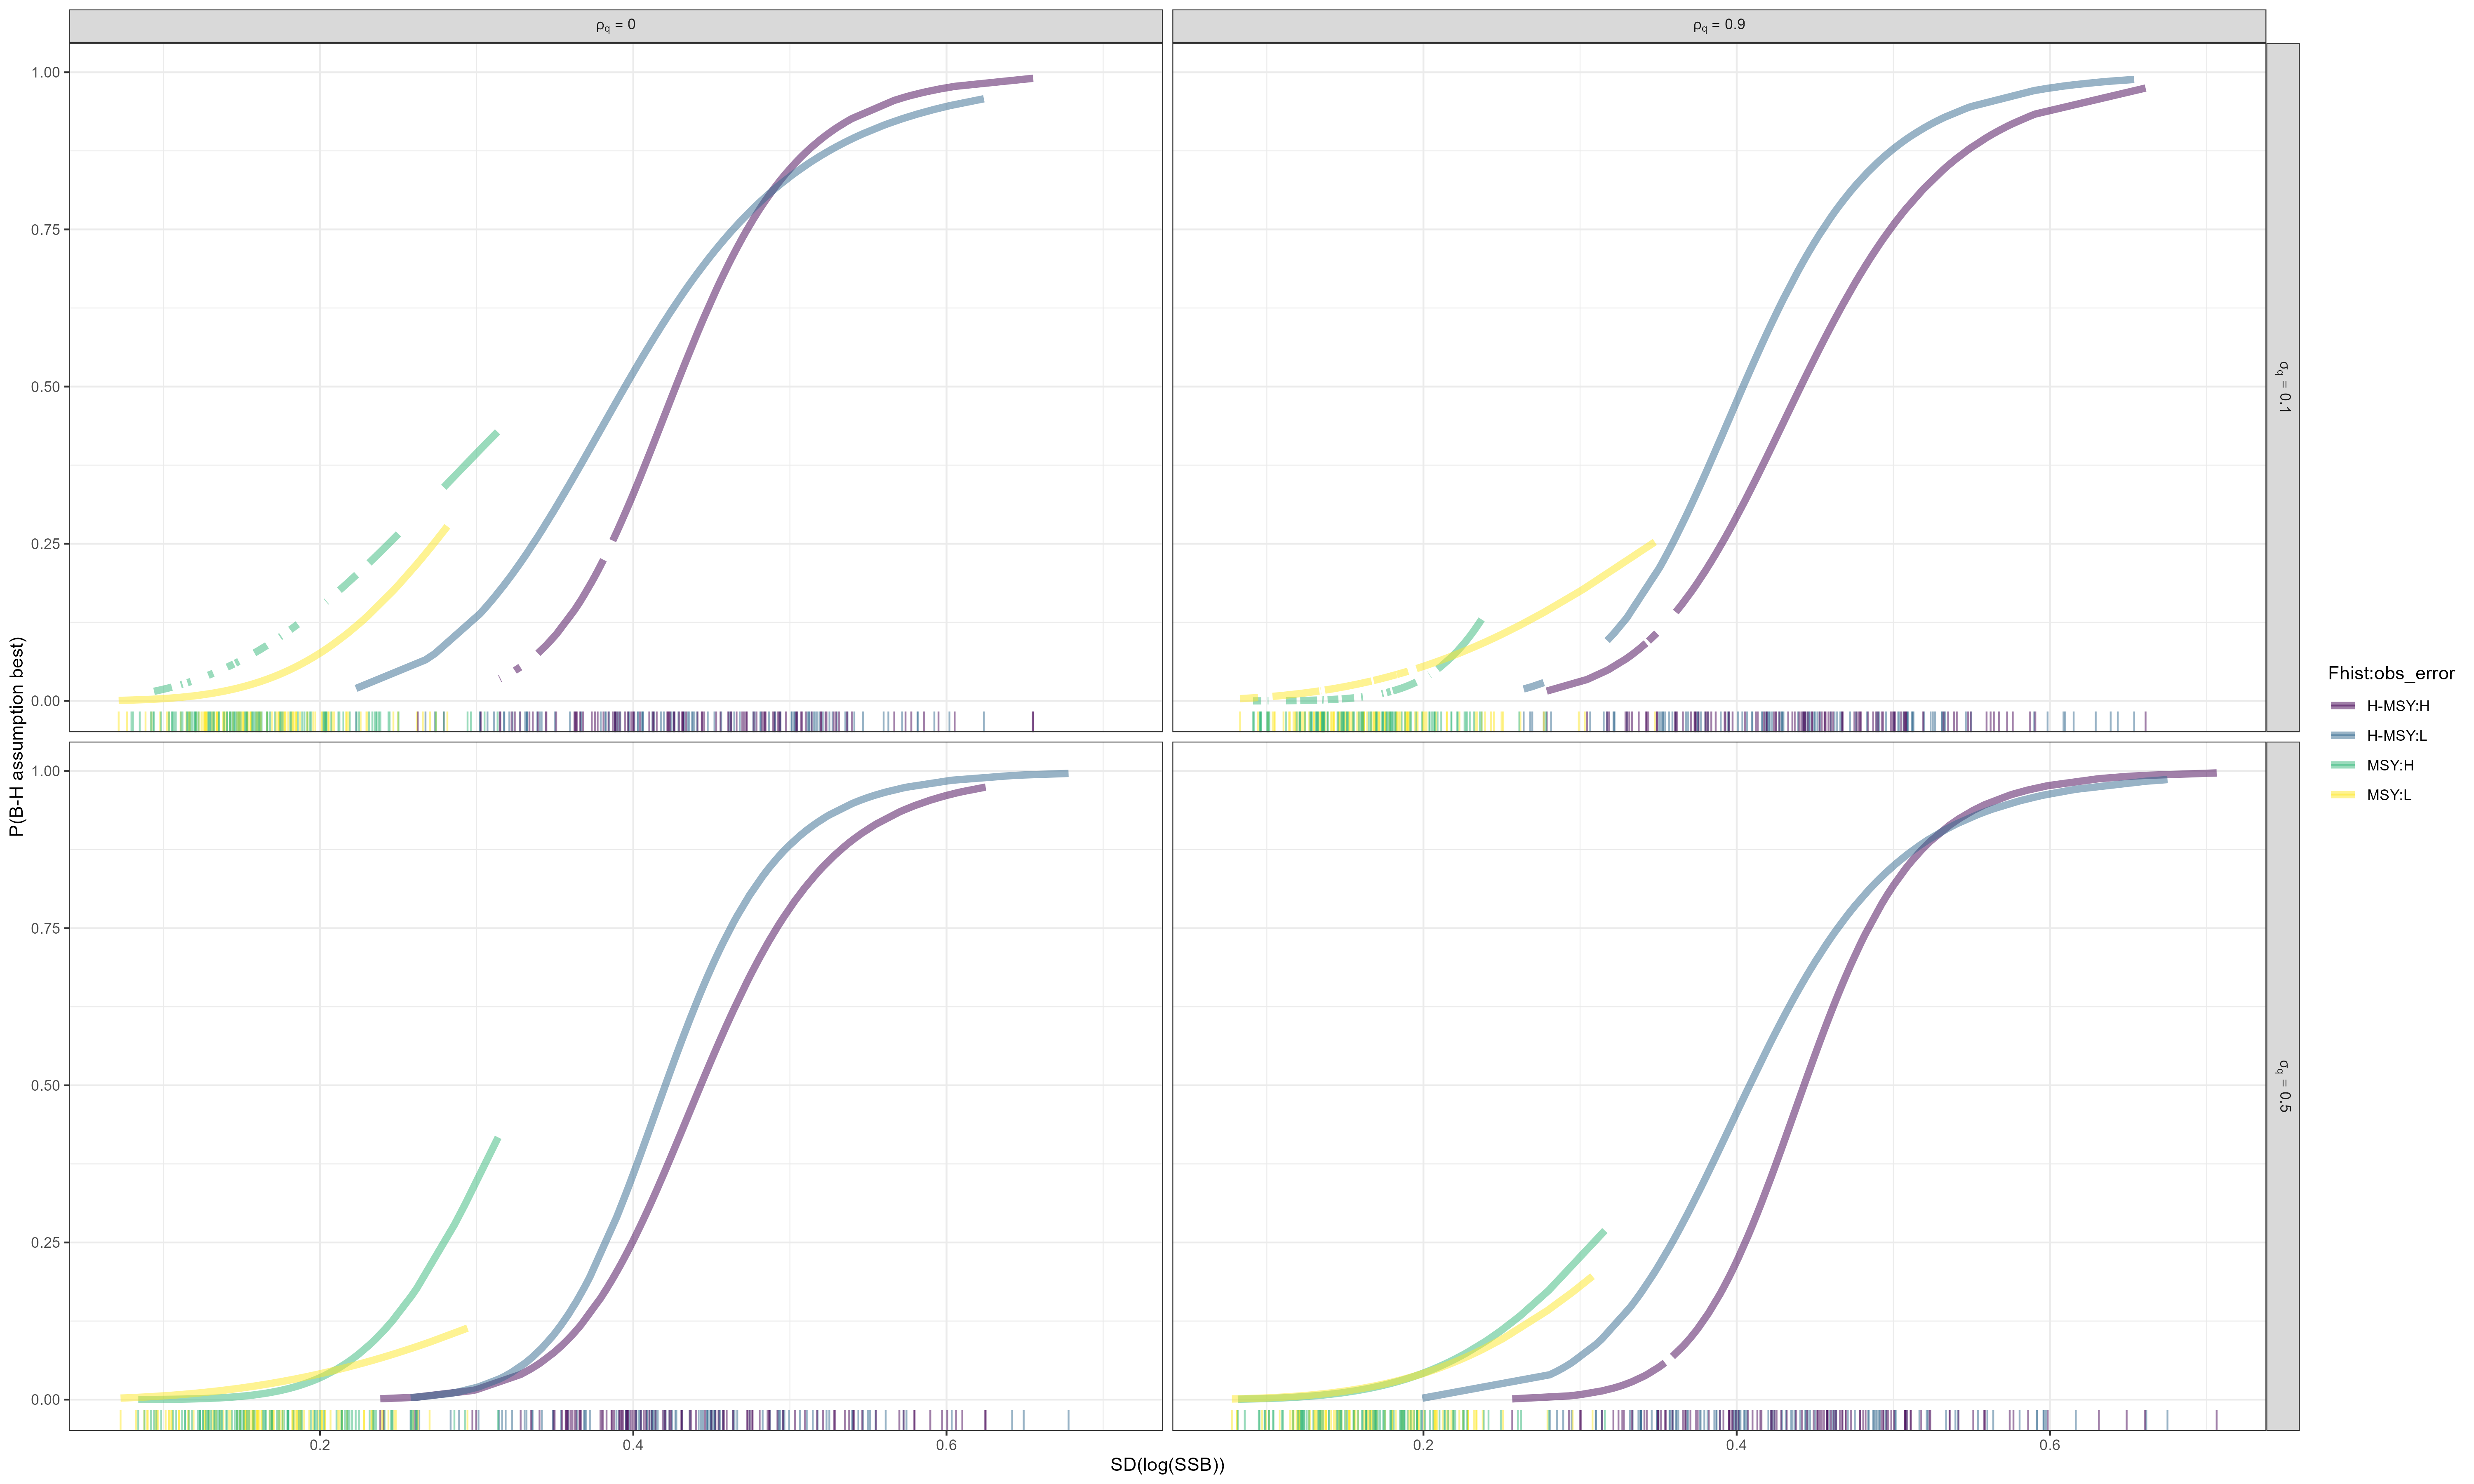
\includegraphics[width = \textwidth]{q_om_MF_pred_BH_best.png}
\end{center}
\end{figure}

\begin{figure}
\caption{Predicted probability of AIC preferring BH model as a function of the variation of population SSB. Operating and estimating models have matching R+q process error structures. Estimating models allow estimation of mean M.}\label{q_om_ME_BH_glm_AIC_plots}
\begin{center}
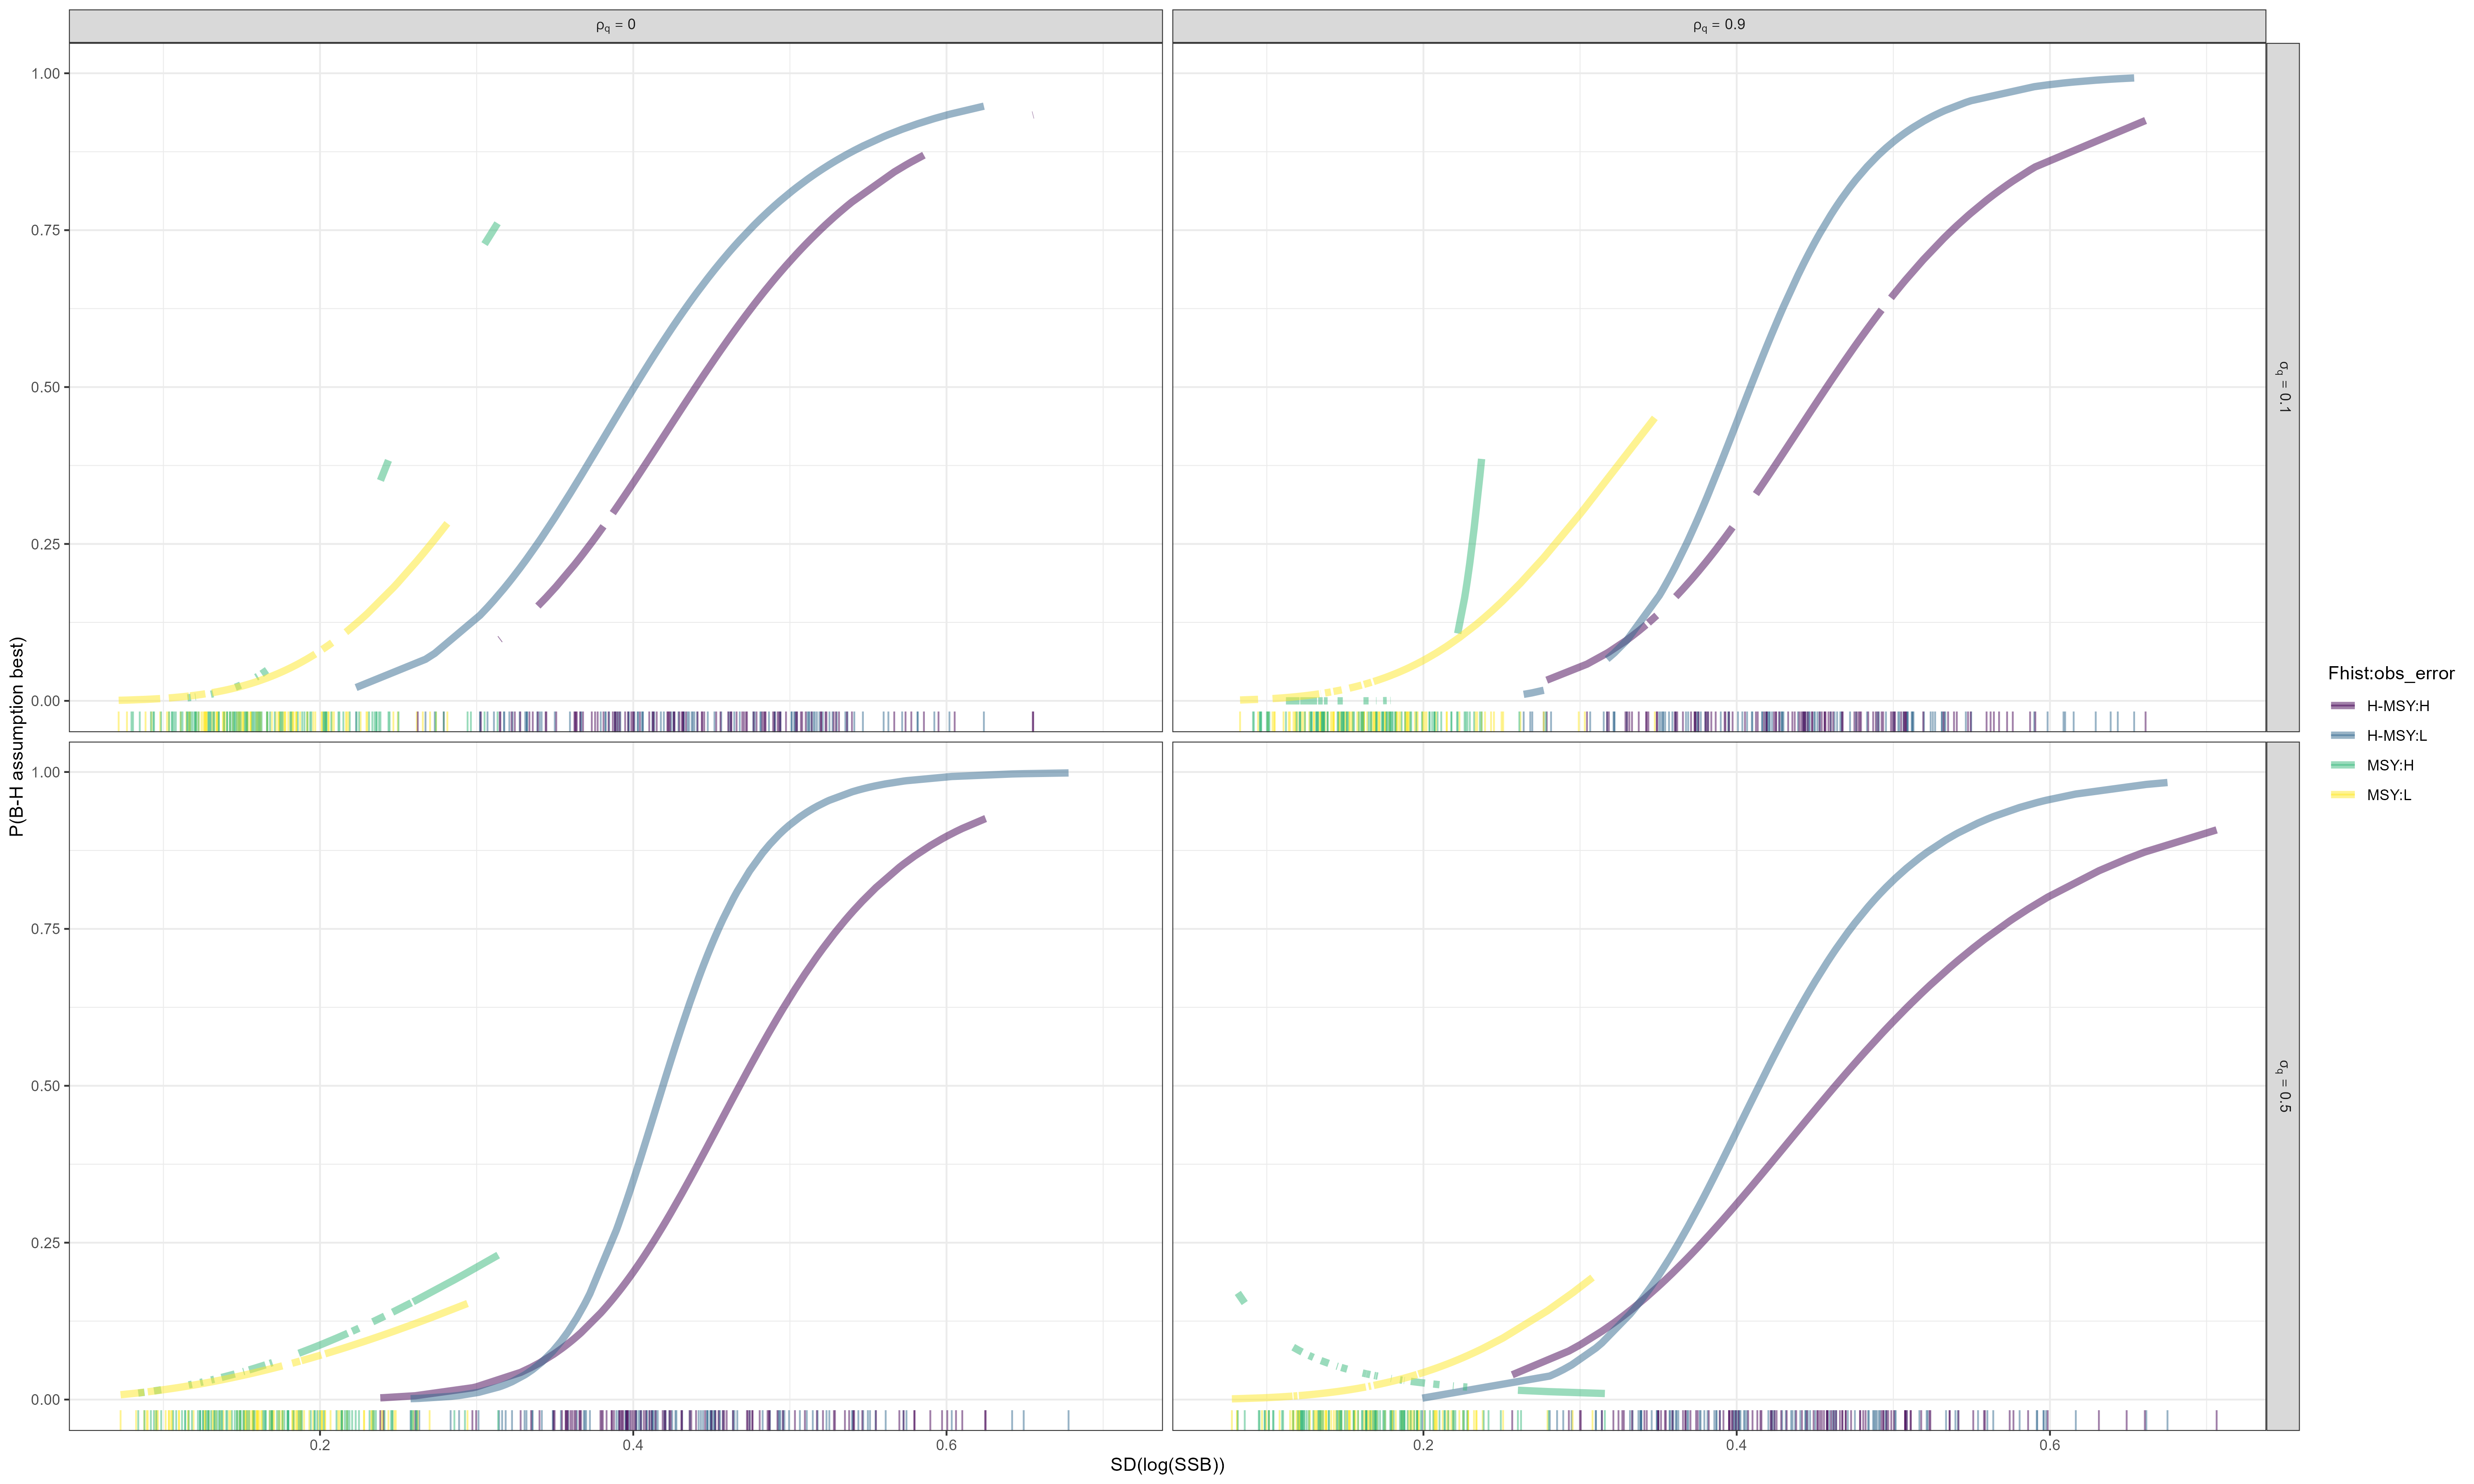
\includegraphics[width = \textwidth]{q_om_ME_pred_BH_best.png}
\end{center}
\end{figure}

\clearpage

\hypertarget{bias-1}{%
\subsection*{Bias}\label{bias-1}}
\addcontentsline{toc}{subsection}{Bias}

\hypertarget{r-rs-oms}{%
\subsubsection*{R, R+S OMs}\label{r-rs-oms}}
\addcontentsline{toc}{subsubsection}{R, R+S OMs}

\begin{landscape}
\begin{figure}
\caption{Median relative bias of SSB for estimating models fitted to data sets simulated with R and R+S process errors.  Estimation models do not assume a stock-recruit function and M is fixed at the true value.}\label{naa_om_em_R_MF_relbias_ssb}
\begin{center}
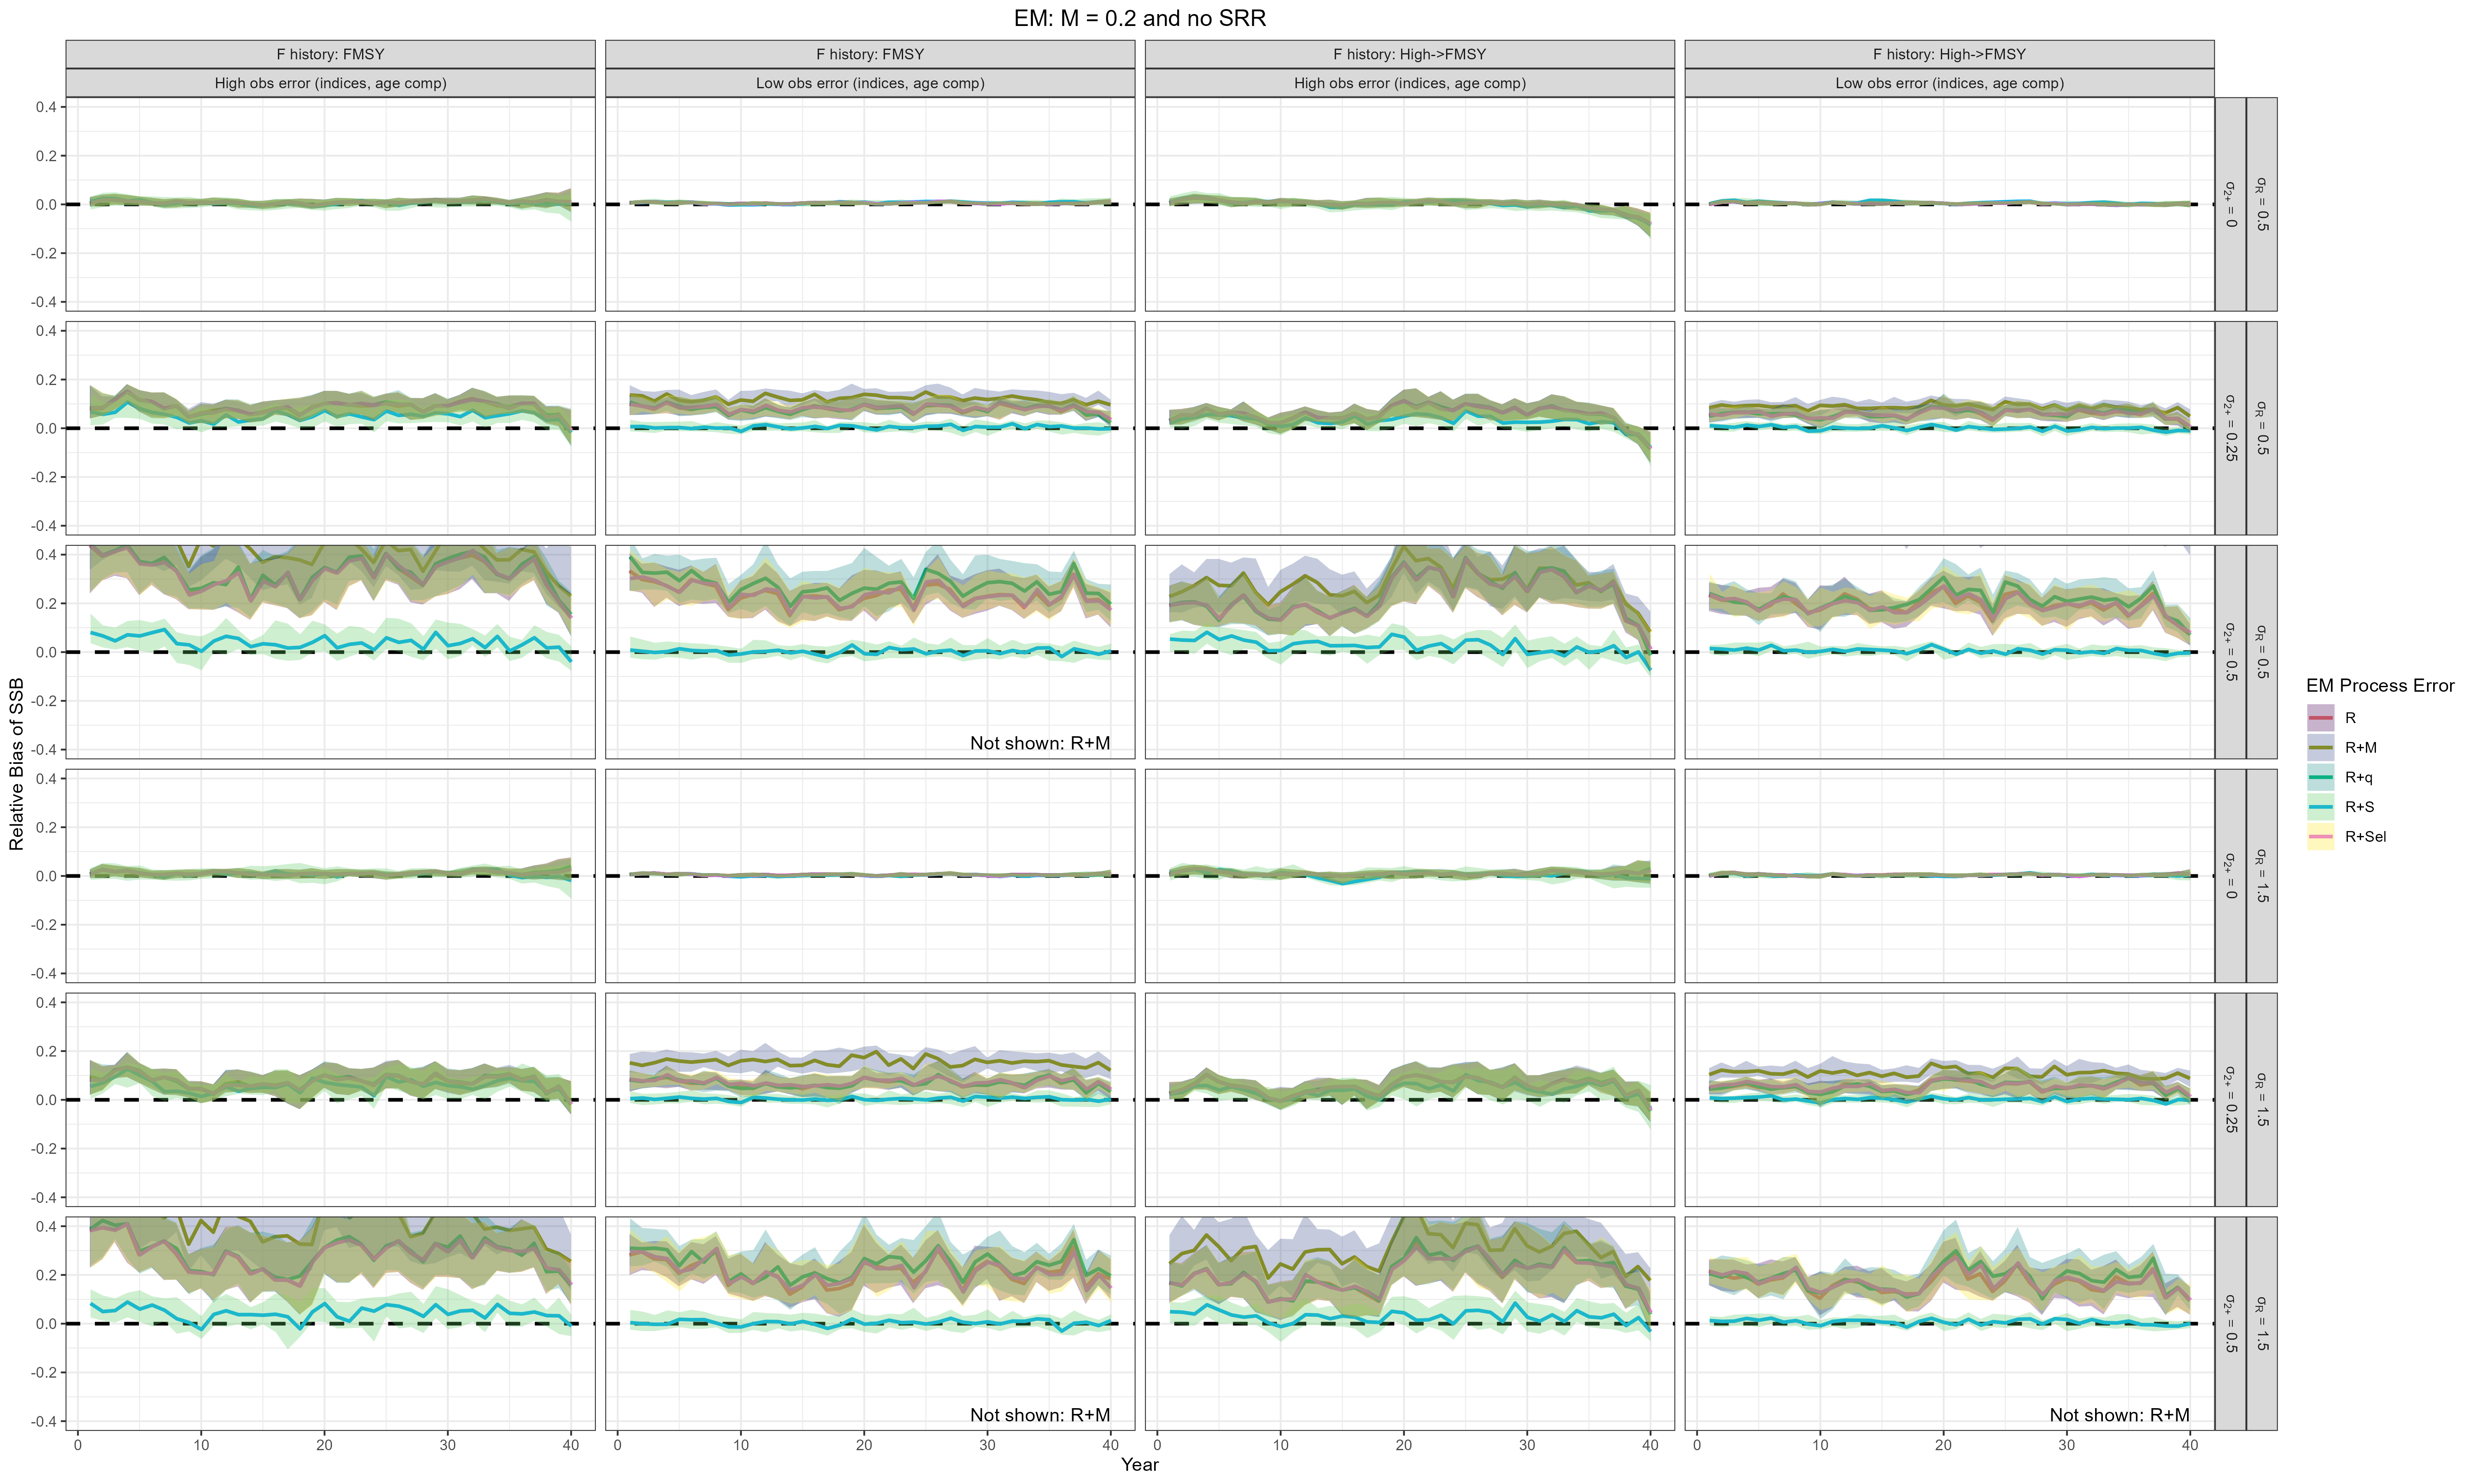
\includegraphics[width = \textwidth]{naa_om_R_MF_relbias_ssb.png}
\end{center}
\end{figure}
\end{landscape}

\begin{landscape}
\begin{figure}
\caption{Median relative bias of SSB for estimating models fitted to data sets simulated with R and R+S process errors. Estimation models do not assume a stock-recruit relationship and estimate M.}\label{naa_om_em_R_ME_relbias_ssb}
\begin{center}
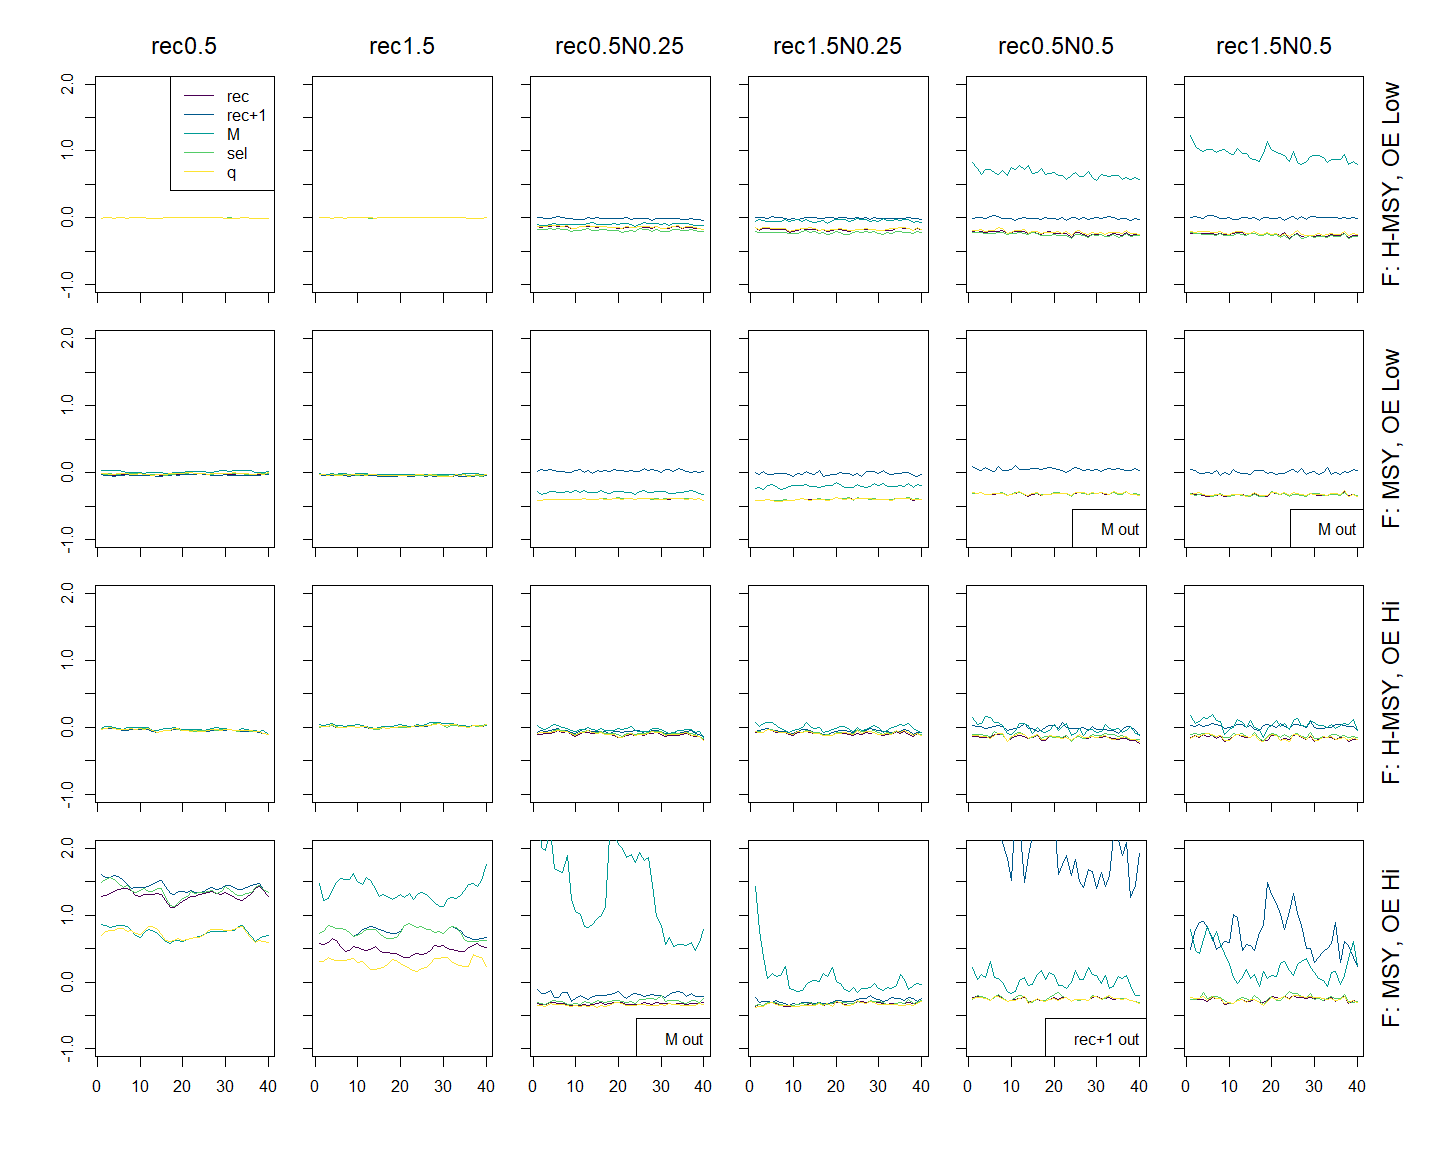
\includegraphics[width = \textwidth]{naa_om_R_ME_relbias_ssb.png}
\end{center}
\end{figure}
\end{landscape}

\begin{landscape}
\begin{figure}
\caption{Median relative bias of SSB for estimating models fitted to data sets simulated with R and R+S process errors. Estimation models assume a BH stock-recruitment function and M is fixed at the true value.}\label{naa_om_em_BH_MF_relbias_ssb}
\begin{center}
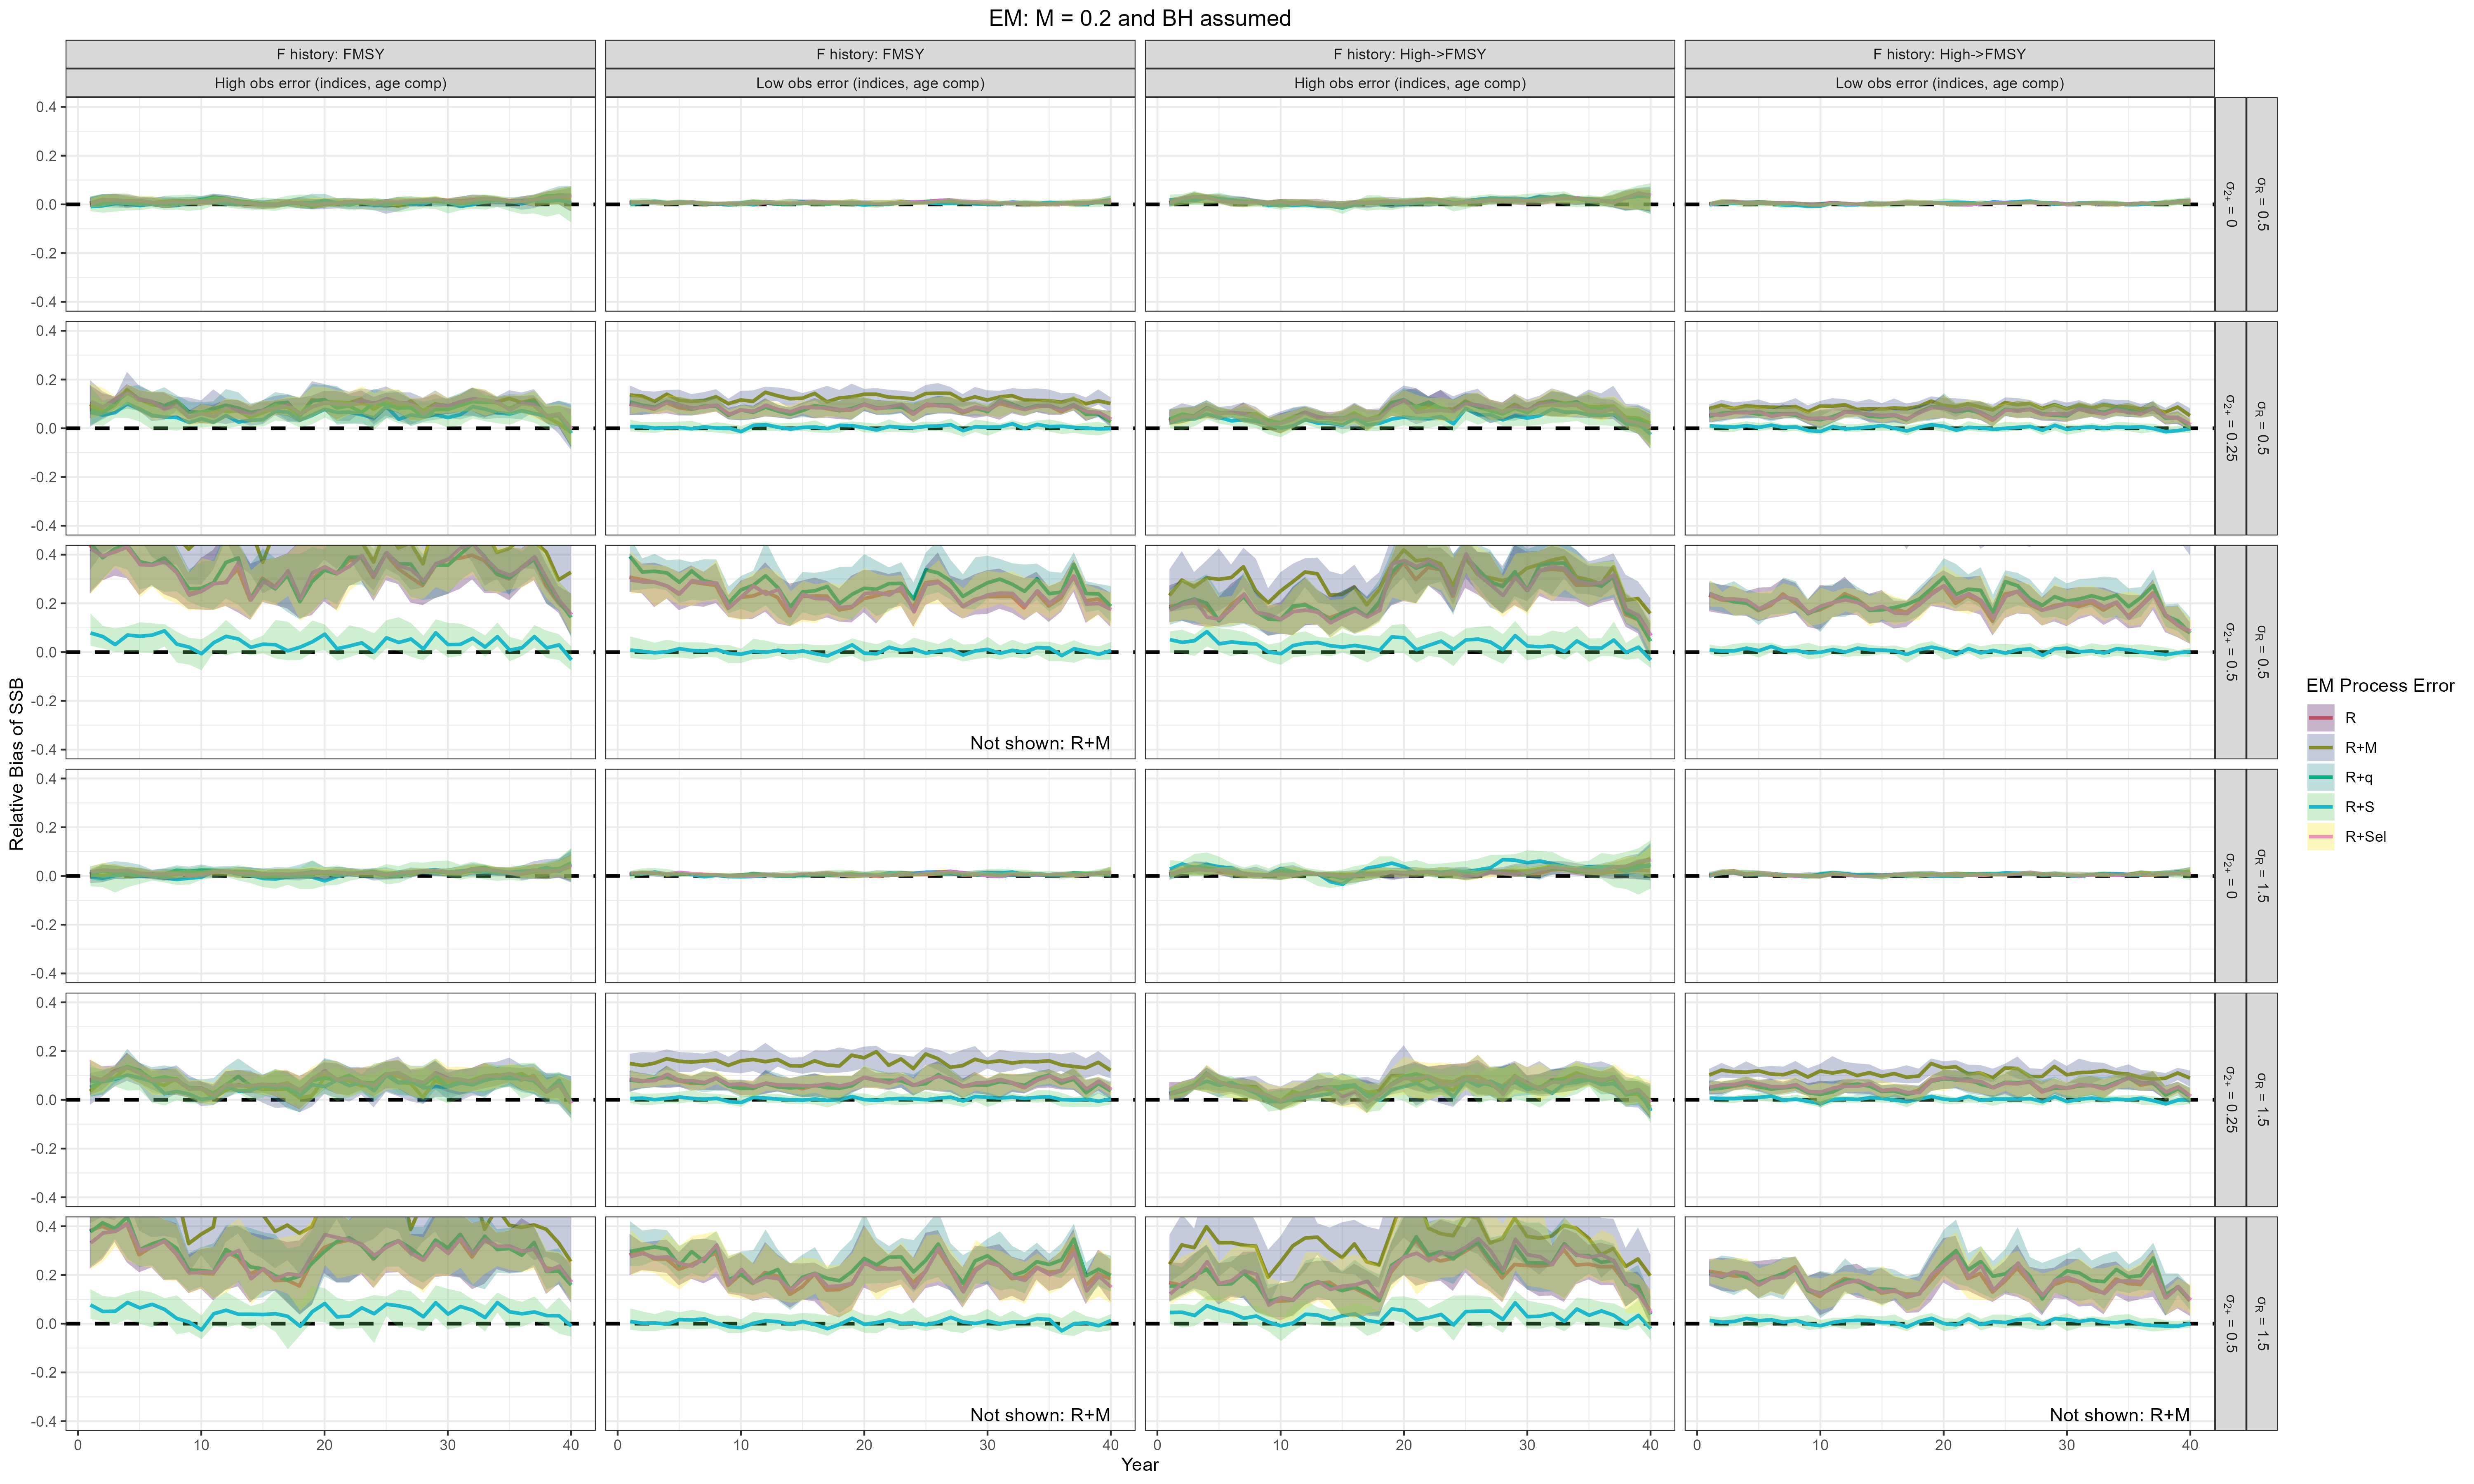
\includegraphics[width = \textwidth]{naa_om_BH_MF_relbias_ssb.png}
\end{center}
\end{figure}
\end{landscape}

\begin{landscape}
\begin{figure}
\caption{Median relative bias of SSB for estimating models fitted to data sets simulated with R and R+S process errors. Estimation models assume a BH stock-recruitment function and estimate M.}\label{naa_om_em_BH_ME_relbias_ssb}
\begin{center}
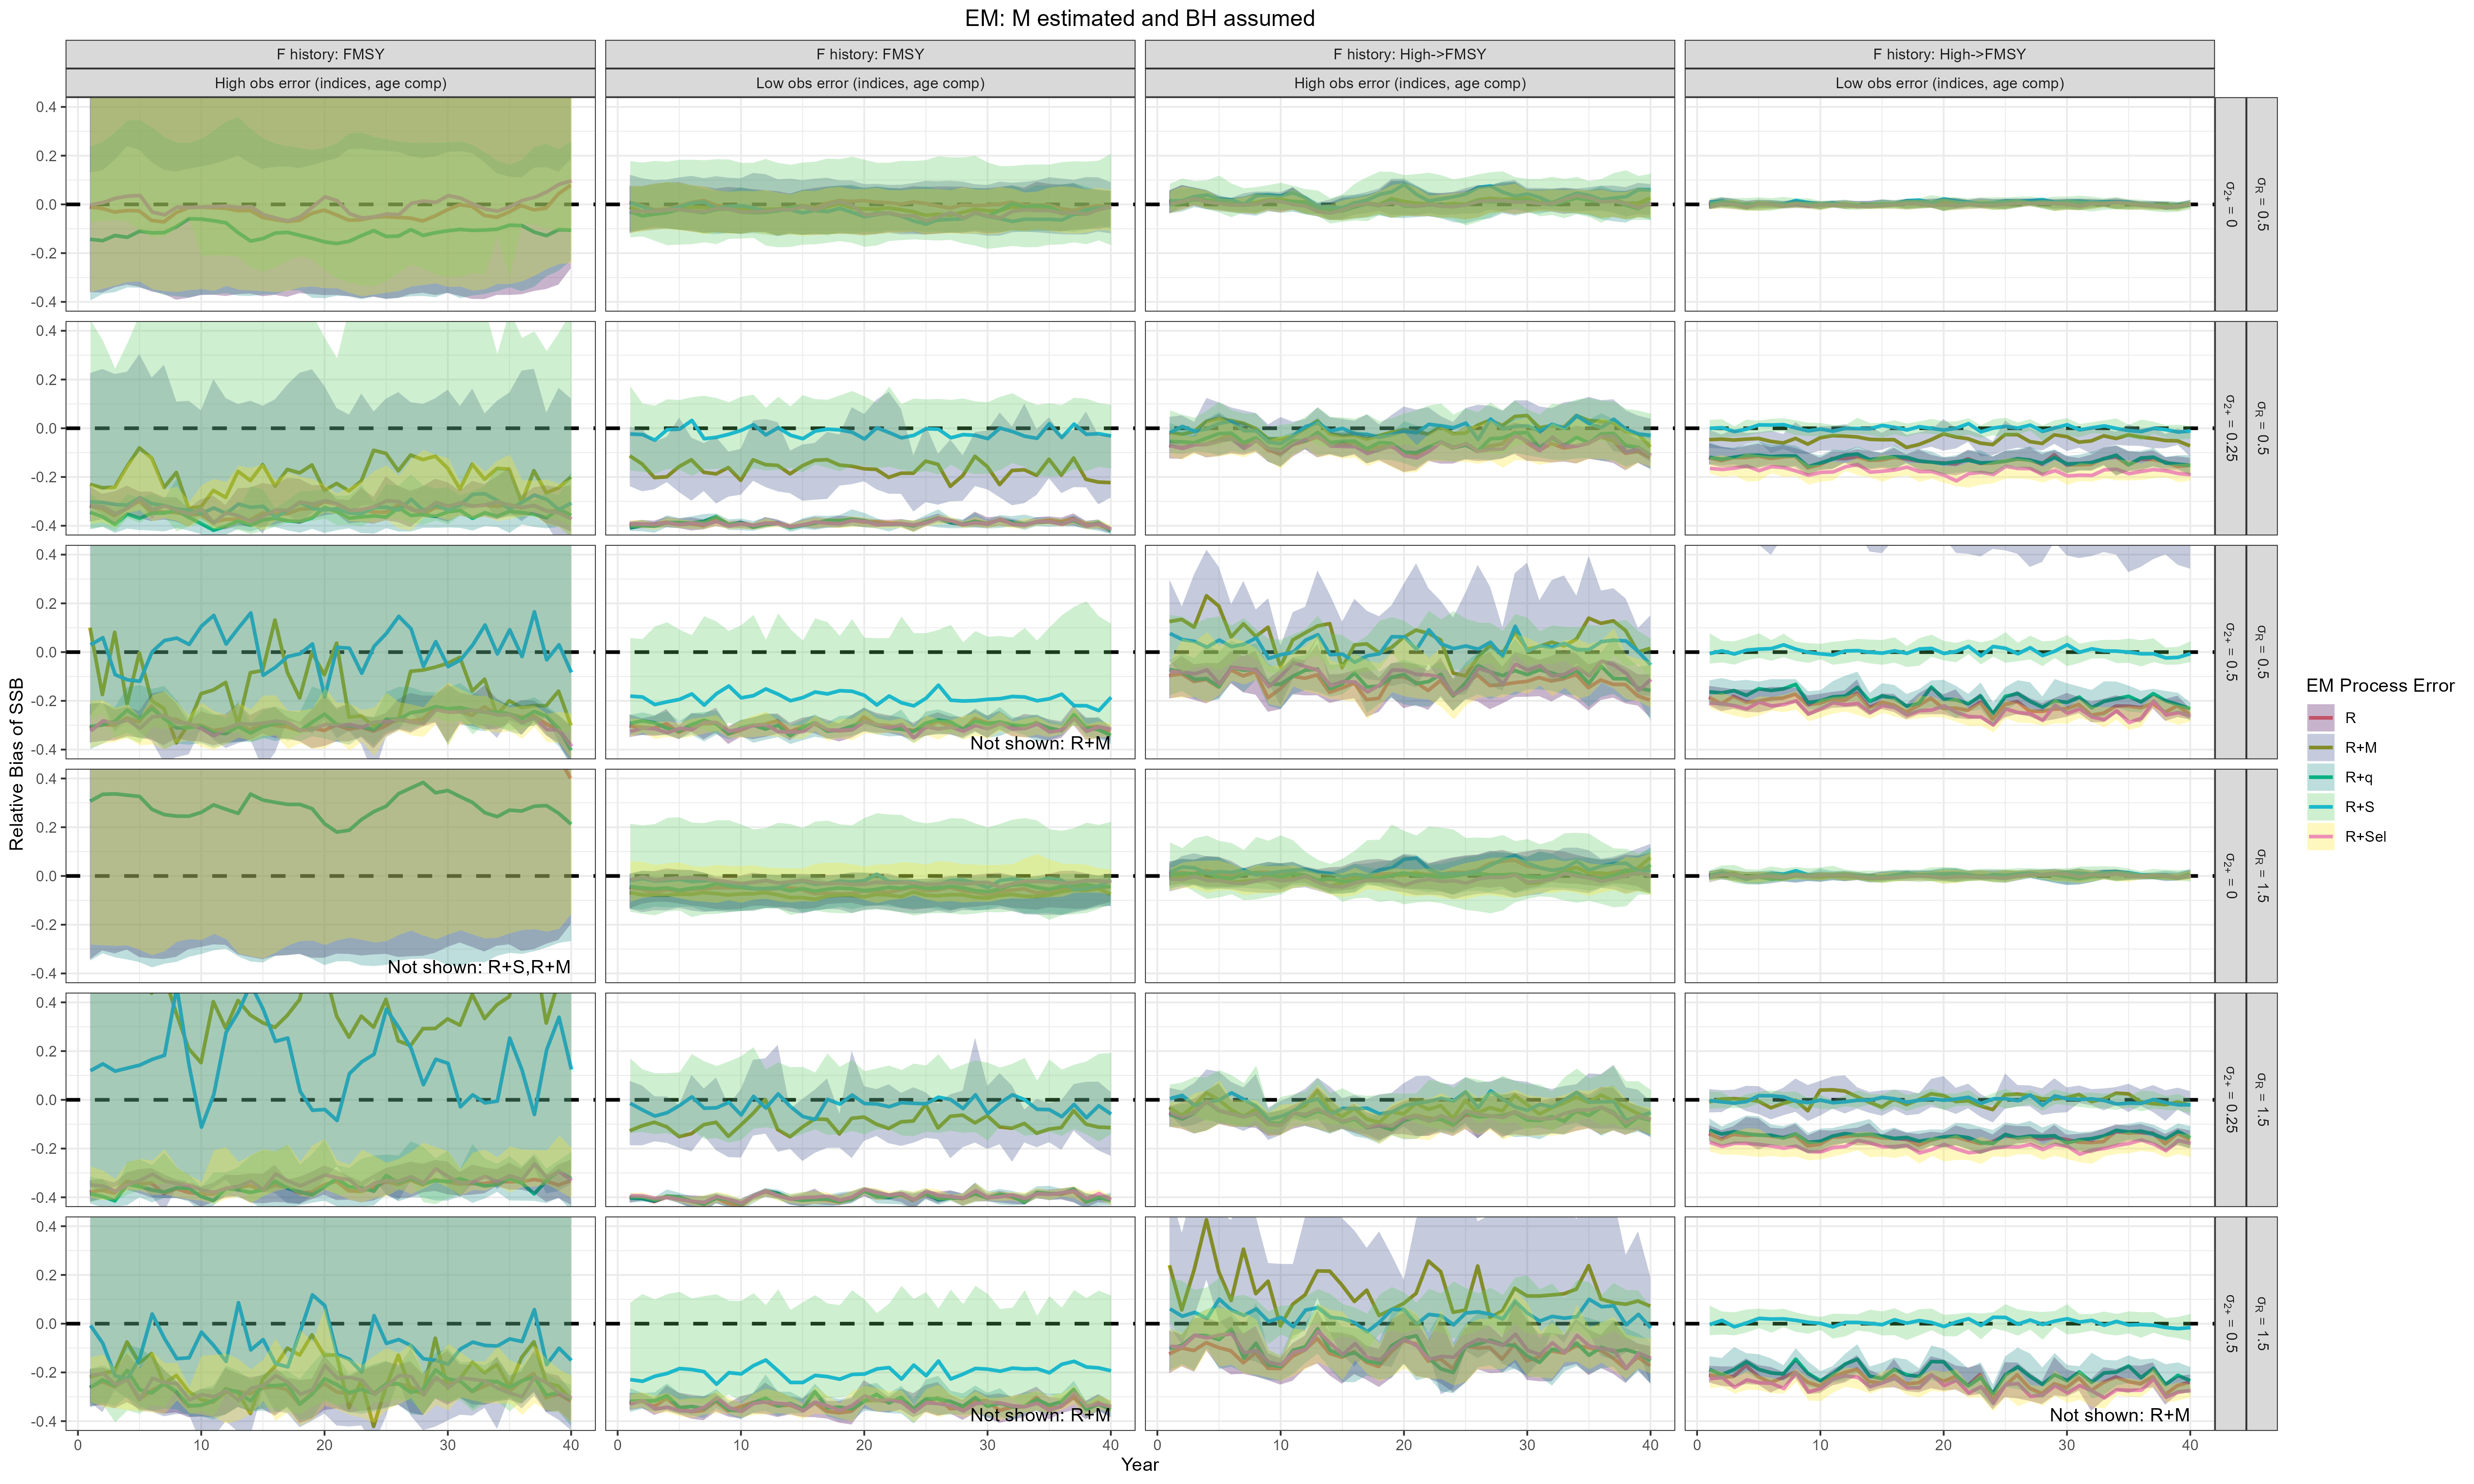
\includegraphics[width = \textwidth]{naa_om_BH_ME_relbias_ssb.png}
\end{center}
\end{figure}
\end{landscape}

\hypertarget{rm-oms}{%
\subsubsection*{R+M OMs}\label{rm-oms}}
\addcontentsline{toc}{subsubsection}{R+M OMs}

\begin{landscape}
\begin{figure}
\caption{Median relative bias of SSB for estimating models fitted to data sets simulated with R+M process errors.  Estimation models do not assume a stock-recruit function and M is fixed at the true value.}\label{M_om_em_R_MF_relbias_ssb}
\begin{center}
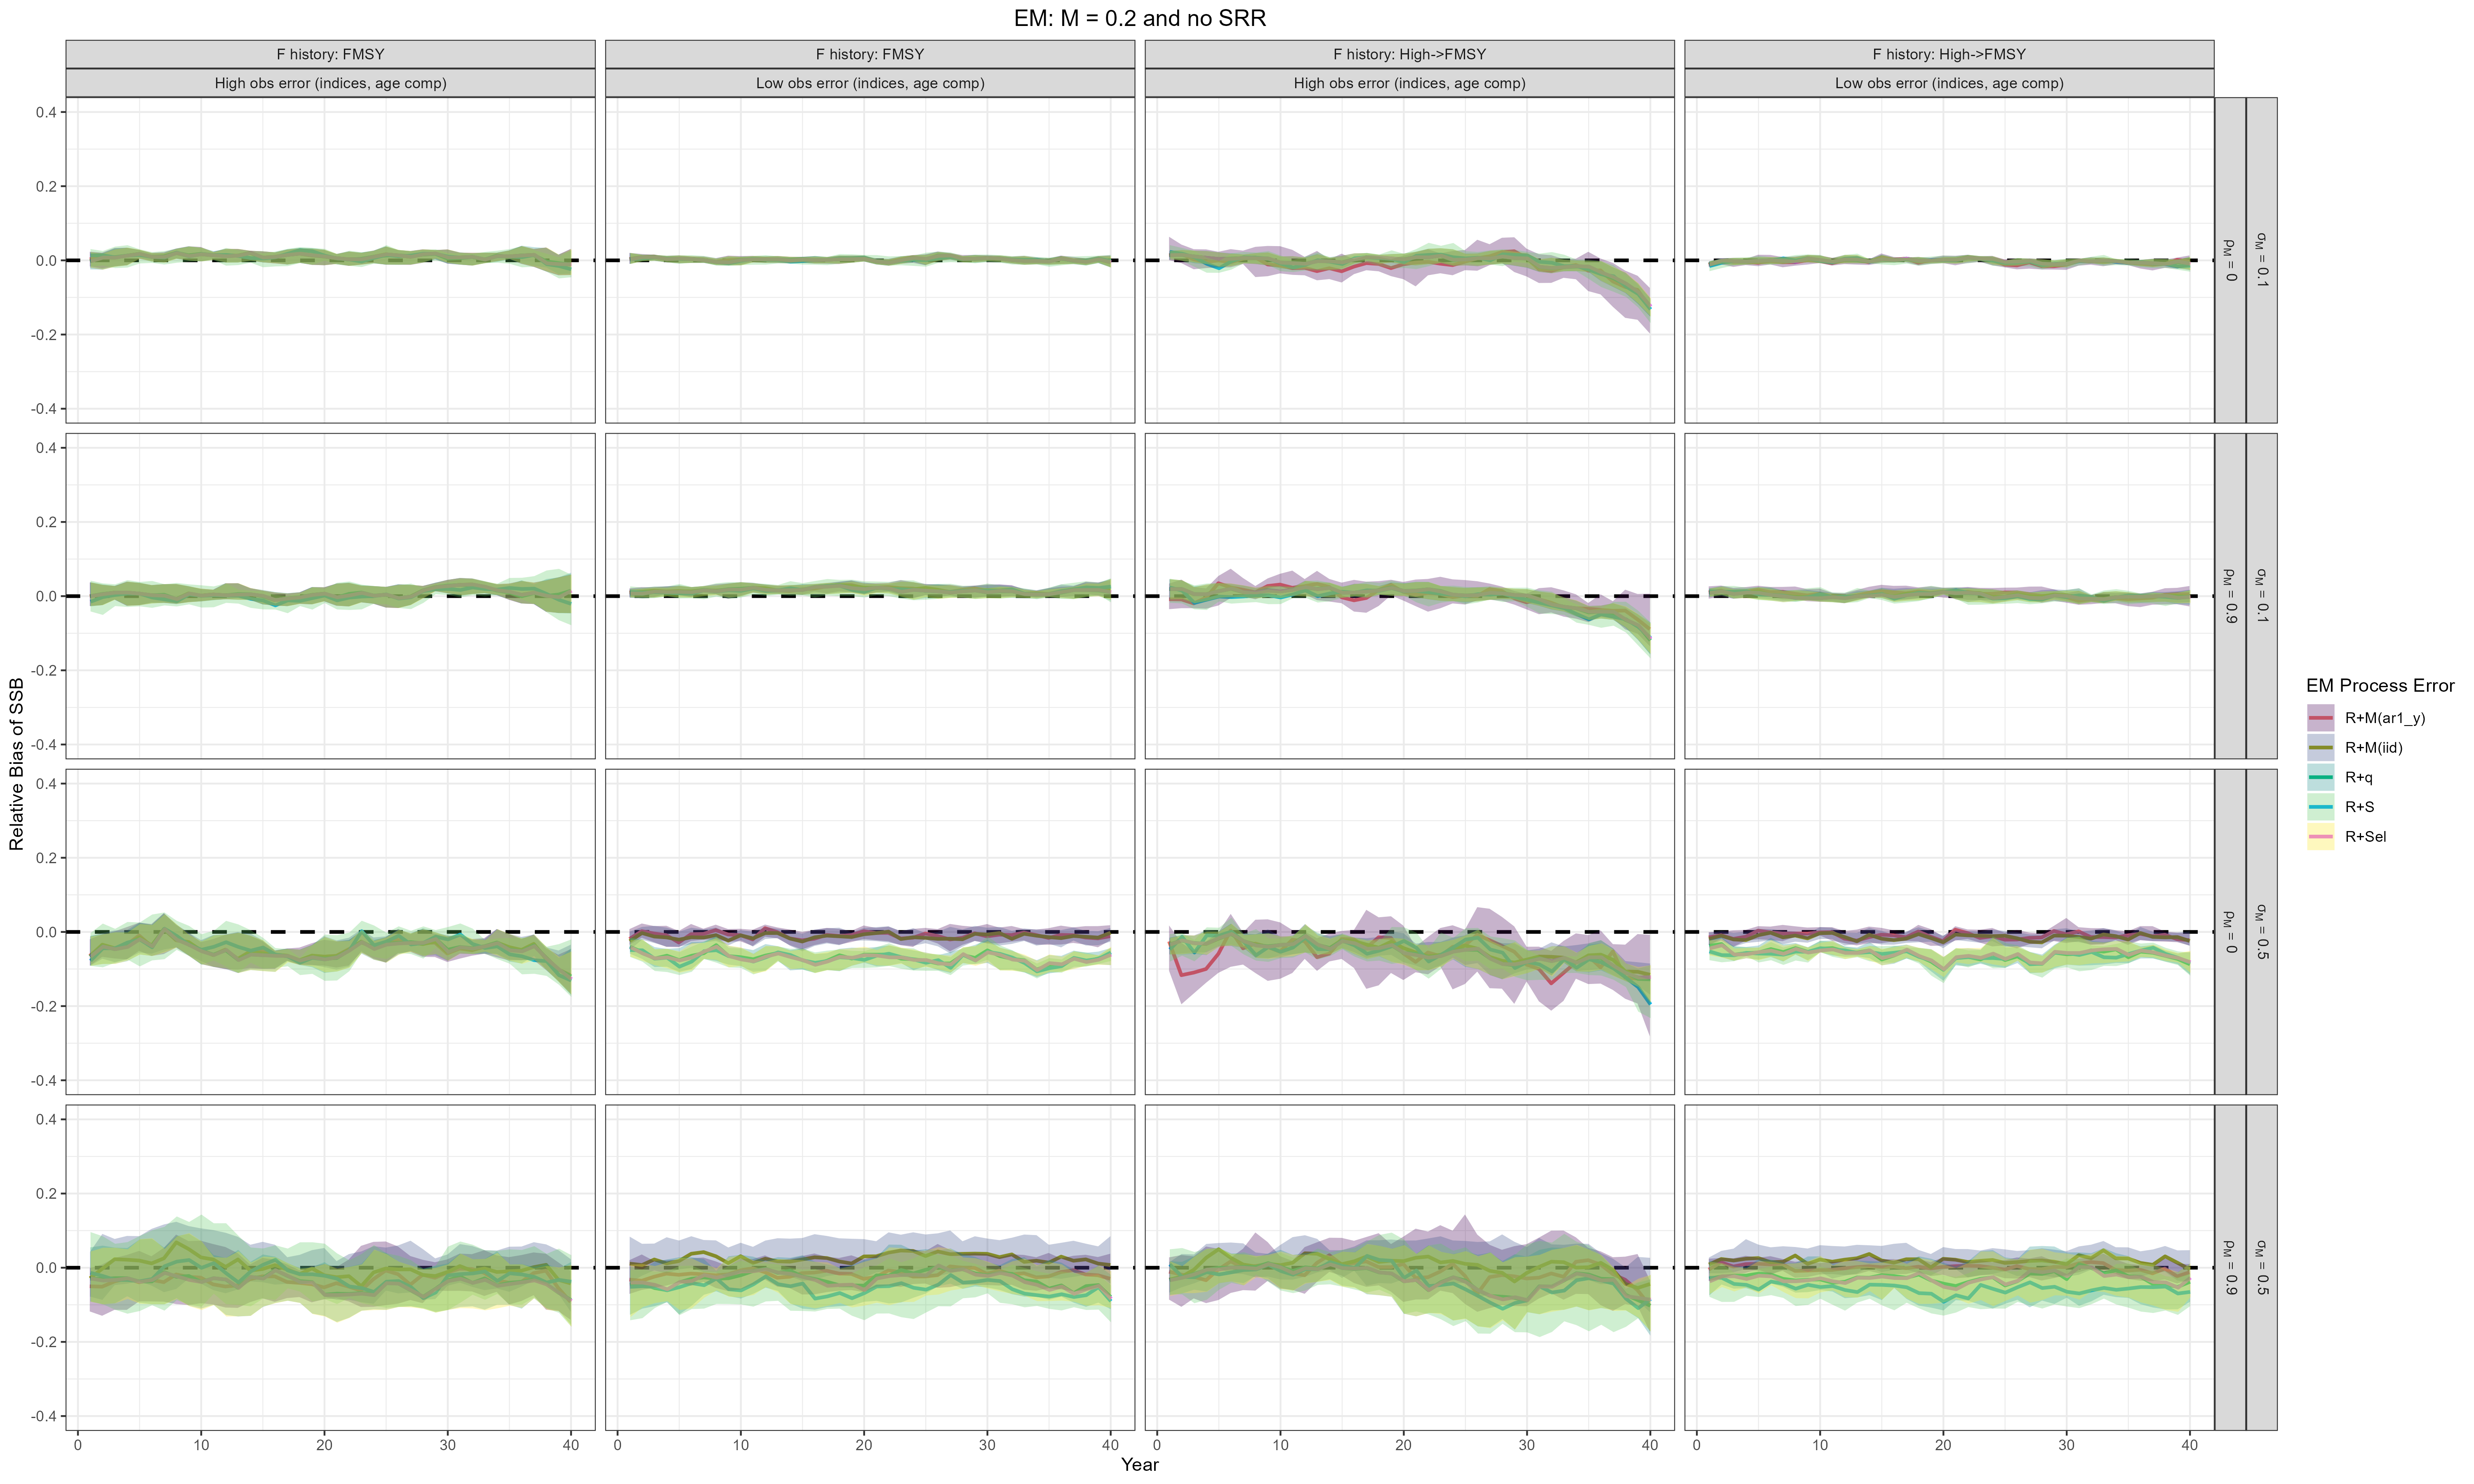
\includegraphics[width = \textwidth]{M_om_R_MF_relbias_ssb.png}
\end{center}
\end{figure}
\end{landscape}

\begin{landscape}
\begin{figure}
\caption{Median relative bias of SSB for estimating models fitted to data sets simulated with R+M process errors. Estimation models do not assume a stock-recruit relationship and estimate M.}\label{M_om_em_R_ME_relbias_ssb}
\begin{center}
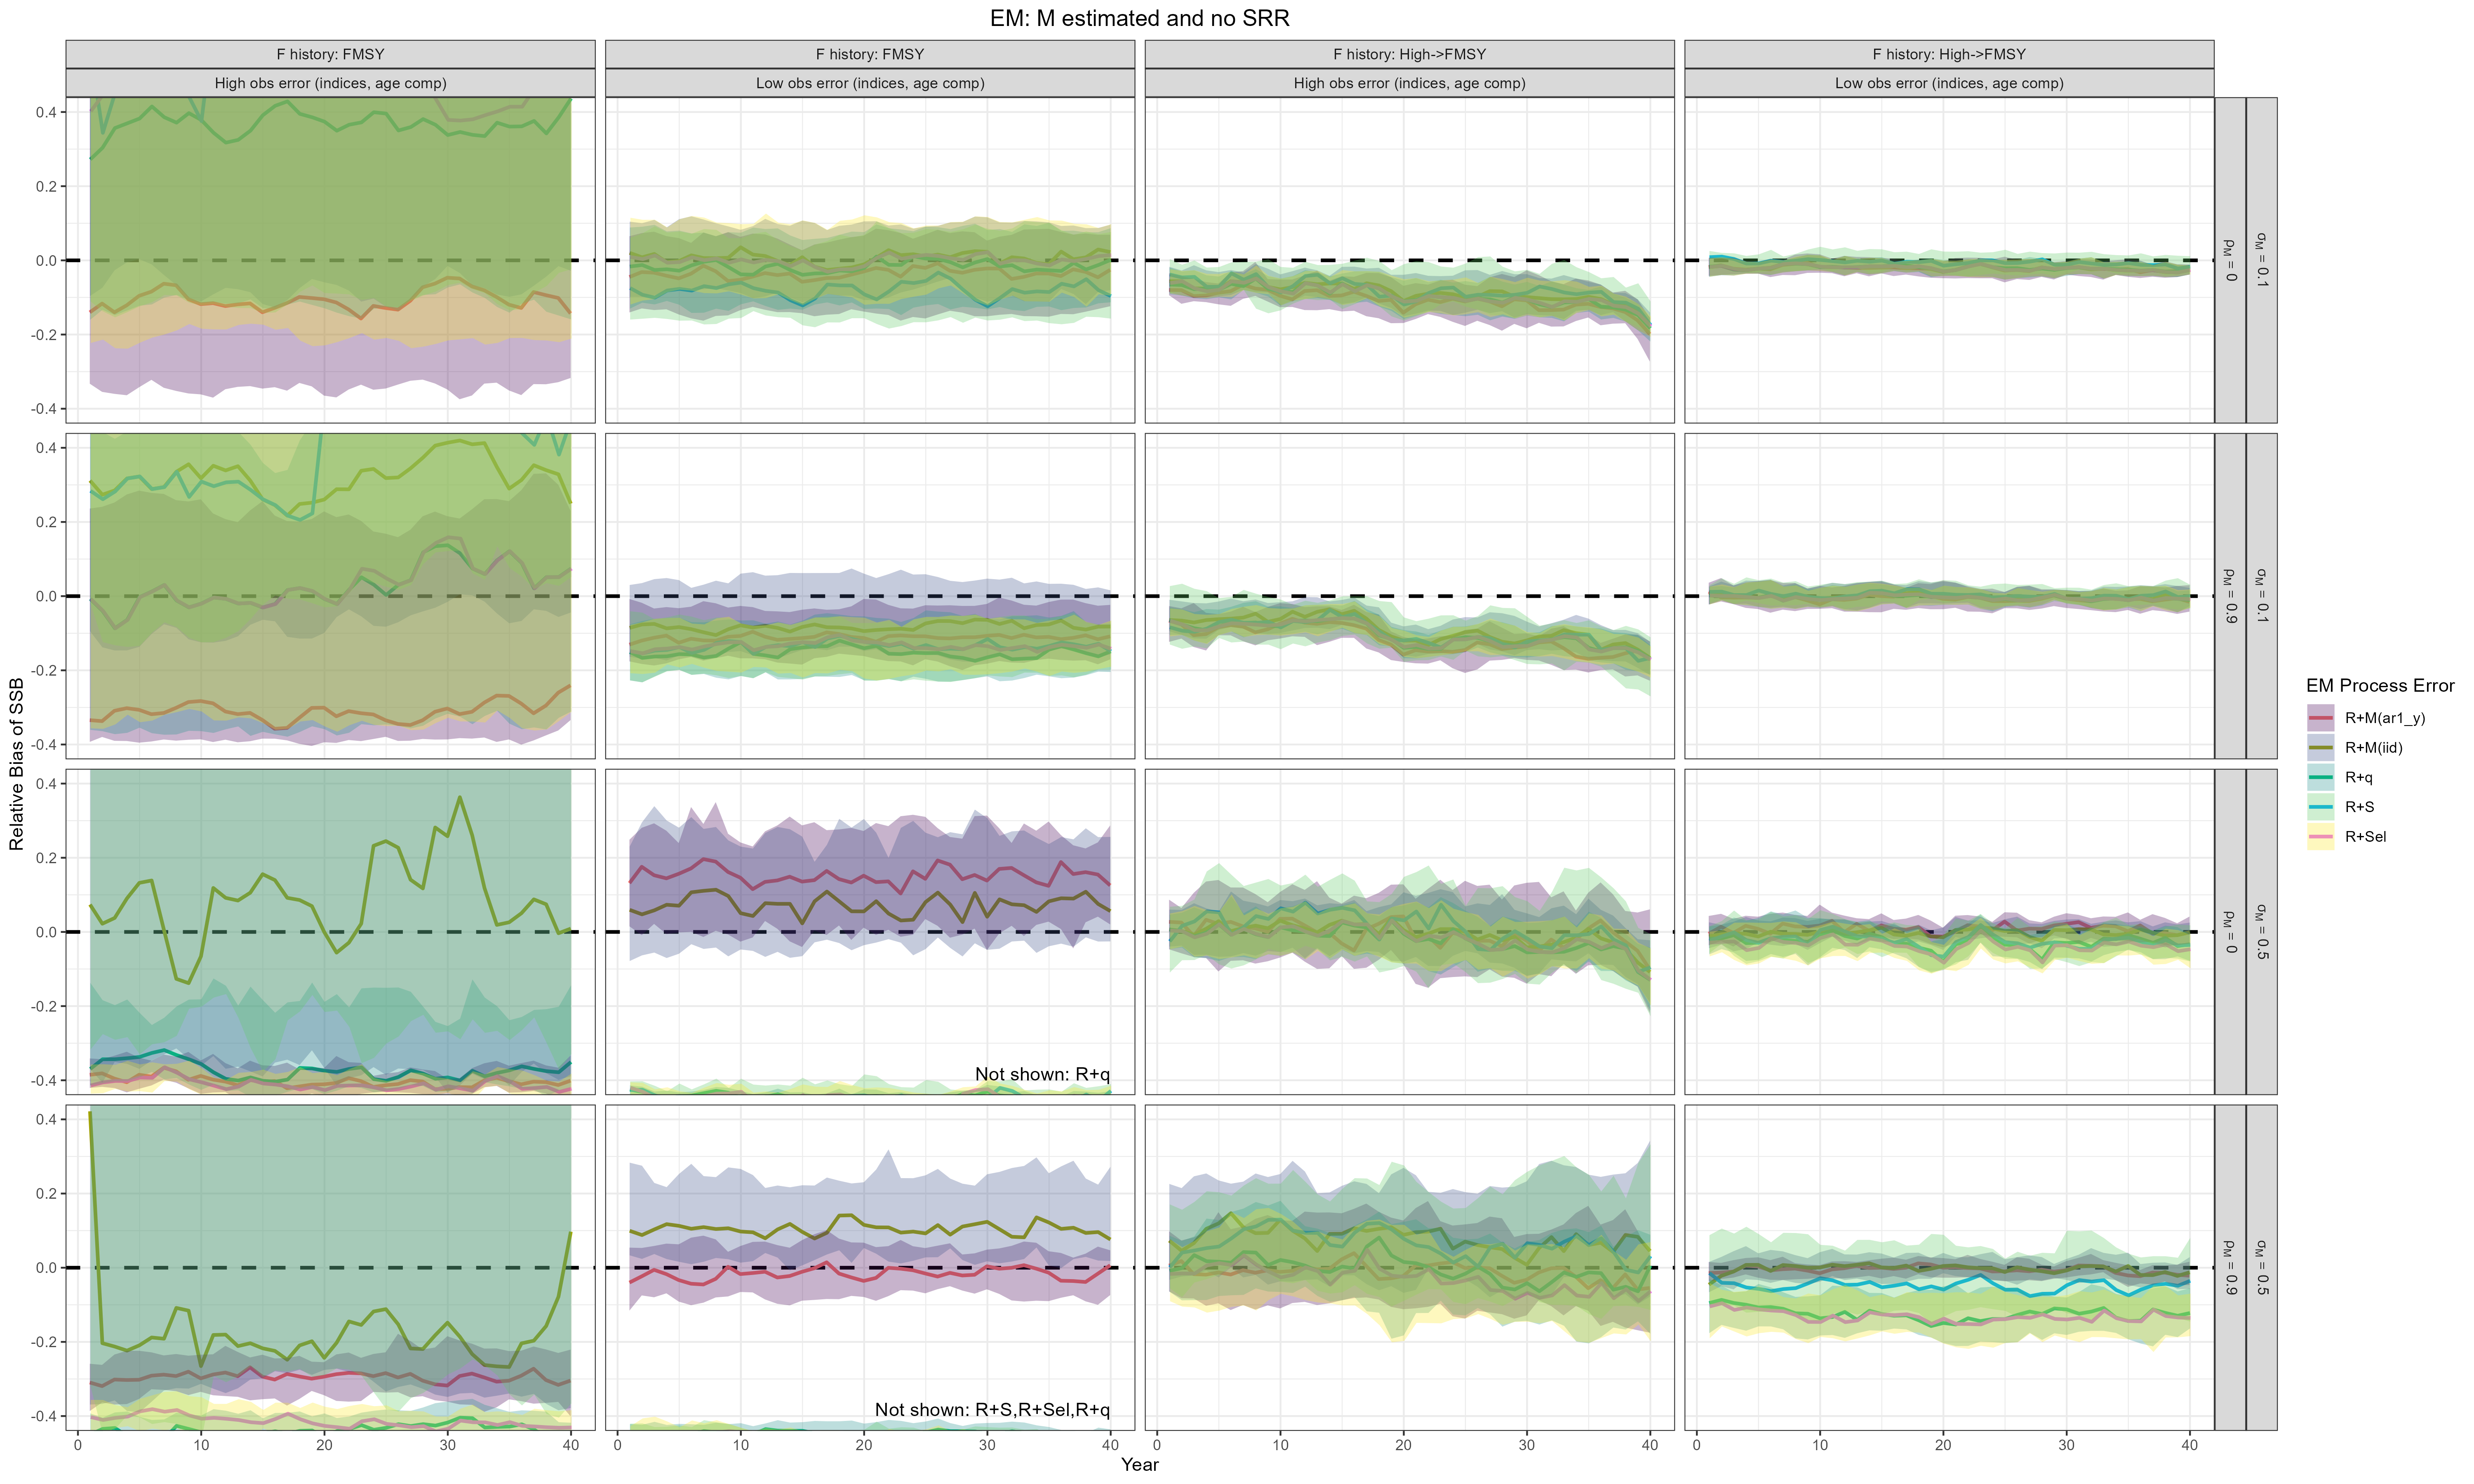
\includegraphics[width = \textwidth]{M_om_R_ME_relbias_ssb.png}
\end{center}
\end{figure}
\end{landscape}

\begin{landscape}
\begin{figure}
\caption{Median relative bias of SSB for estimating models fitted to data sets simulated with R+M process errors. Estimation models assume a BH stock-recruitment function and M is fixed at the true value.}\label{M_om_em_BH_MF_relbias_ssb}
\begin{center}
\includegraphics[width = \textwidth]{M_om_BH_MF_relbias_ssb.png}
\end{center}
\end{figure}
\end{landscape}

\begin{landscape}
\begin{figure}
\caption{Median relative bias of SSB for estimating models fitted to data sets simulated with R+M process errors. Estimation models assume a BH stock-recruitment function and estimate M.}\label{M_om_em_BH_ME_relbias_ssb}
\begin{center}
\includegraphics[width = \textwidth]{M_om_BH_ME_relbias_ssb.png}
\end{center}
\end{figure}
\end{landscape}

\hypertarget{rsel-oms}{%
\subsubsection*{R+Sel OMs}\label{rsel-oms}}
\addcontentsline{toc}{subsubsection}{R+Sel OMs}

\begin{landscape}
\begin{figure}
\caption{Median relative bias of SSB for estimating models fitted to data sets simulated with R+Sel process errors.  Estimation models do not assume a stock-recruit function and M is fixed at the true value.}\label{Sel_om_em_R_MF_relbias_ssb}
\begin{center}
\includegraphics[width = \textwidth]{Sel_om_R_MF_relbias_ssb.png}
\end{center}
\end{figure}
\end{landscape}

\begin{landscape}
\begin{figure}
\caption{Median relative bias of SSB for estimating models fitted to data sets simulated with R+Sel process errors. Estimation models do not assume a stock-recruit relationship and estimate M.}\label{Sel_om_em_R_ME_relbias_ssb}
\begin{center}
\includegraphics[width = \textwidth]{Sel_om_R_ME_relbias_ssb.png}
\end{center}
\end{figure}
\end{landscape}

\begin{landscape}
\begin{figure}
\caption{Median relative bias of SSB for estimating models fitted to data sets simulated with R+Sel process errors. Estimation models assume a BH stock-recruitment function and M is fixed at the true value.}\label{Sel_om_em_BH_MF_relbias_ssb}
\begin{center}
\includegraphics[width = \textwidth]{Sel_om_BH_MF_relbias_ssb.png}
\end{center}
\end{figure}
\end{landscape}

\begin{landscape}
\begin{figure}
\caption{Median relative bias of SSB for estimating models fitted to data sets simulated with R+Sel process errors. Estimation models assume a BH stock-recruitment function and estimate M.}\label{Sel_om_em_BH_ME_relbias_ssb}
\begin{center}
\includegraphics[width = \textwidth]{Sel_om_BH_ME_relbias_ssb.png}
\end{center}
\end{figure}
\end{landscape}

\hypertarget{rq-oms}{%
\subsubsection*{R+q OMs}\label{rq-oms}}
\addcontentsline{toc}{subsubsection}{R+q OMs}

\begin{landscape}
\begin{figure}
\caption{Median relative bias of SSB for estimating models fitted to data sets simulated with R+q process errors.  Estimation models do not assume a stock-recruit function and M is fixed at the true value.}\label{q_om_em_R_MF_relbias_ssb}
\begin{center}
\includegraphics[width = \textwidth]{q_om_R_MF_relbias_ssb.png}
\end{center}
\end{figure}
\end{landscape}

\begin{landscape}
\begin{figure}
\caption{Median relative bias of SSB for estimating models fitted to data sets simulated with R+q process errors. Estimation models do not assume a stock-recruit relationship and estimate M.}\label{q_om_em_R_ME_relbias_ssb}
\begin{center}
\includegraphics[width = \textwidth]{q_om_R_ME_relbias_ssb.png}
\end{center}
\end{figure}
\end{landscape}

\begin{landscape}
\begin{figure}
\caption{Median relative bias of SSB for estimating models fitted to data sets simulated with R+q process errors. Estimation models assume a BH stock-recruitment function and M is fixed at the true value.}\label{q_om_em_BH_MF_relbias_ssb}
\begin{center}
\includegraphics[width = \textwidth]{q_om_BH_MF_relbias_ssb.png}
\end{center}
\end{figure}
\end{landscape}

\begin{landscape}
\begin{figure}
\caption{Median relative bias of SSB for estimating models fitted to data sets simulated with R+q process errors. Estimation models assume a BH stock-recruitment function and estimate M.}\label{q_om_em_BH_ME_relbias_ssb}
\begin{center}
\includegraphics[width = \textwidth]{q_om_BH_ME_relbias_ssb.png}
\end{center}
\end{figure}
\end{landscape}

\hypertarget{beverton-holt-parameter-estimation}{%
\subsubsection{Beverton-Holt parameter
estimation}\label{beverton-holt-parameter-estimation}}

\begin{landscape}
\begin{figure}
\caption{Median relative error of Beverton-Holt stock recruit parameters for estimating models with correct process error assumptions fitted to data sets simulated with R and R+S process errors. Estimation models either assume the correct natural mortality rate or estimate it.}\label{naa_om_SR_relbias}
\begin{center}
\includegraphics[width = \textwidth]{naa_om_SR_relerror.png}
\end{center}
\end{figure}
\end{landscape}

\begin{landscape}
\begin{figure}
\caption{Median relative error of Beverton-Holt stock recruit parameters for estimating models with correct process error assumptions fitted to data sets simulated with R+M process errors. Estimation models either assume the correct natural mortality rate or estimate it.}\label{M_om_SR_relbias}
\begin{center}
\includegraphics[width = \textwidth]{M_om_SR_relerror.png}
\end{center}
\end{figure}
\end{landscape}

\begin{landscape}
\begin{figure}
\caption{Median relative error of Beverton-Holt stock recruit parameters for estimating models with correct process error assumptions fitted to data sets simulated with R+Sel process errors. Estimation models either assume the correct natural mortality rate or estimate it.}\label{Sel_om_SR_relbias}
\begin{center}
\includegraphics[width = \textwidth]{Sel_om_SR_relerror.png}
\end{center}
\end{figure}
\end{landscape}

\begin{landscape}
\begin{figure}
\caption{Median relative error of Beverton-Holt stock recruit parameters for estimating models with correct process error assumptions fitted to data sets simulated with R+q process errors. Estimation models either assume the correct natural mortality rate or estimate it.}\label{q_om_SR_relbias}
\begin{center}
\includegraphics[width = \textwidth]{q_om_SR_relerror.png}
\end{center}
\end{figure}
\end{landscape}

\hypertarget{mean-natural-mortality-rate-estimation}{%
\subsubsection{(Mean) natural mortality rate
estimation}\label{mean-natural-mortality-rate-estimation}}

\begin{landscape}
\begin{figure}
\caption{Median relative error of (mean) natural mortality rate for estimating models with correct process error assumptions fitted to data sets simulated with R and R+S process errors. Estimation models assumed either no stock-recruit relationship or estimated a Beverton-Holt relationship.}\label{naa_om_M_relbias}
\begin{center}
\includegraphics[width = \textwidth]{naa_om_M_relerror.png}
\end{center}
\end{figure}
\end{landscape}

\begin{landscape}
\begin{figure}
\caption{Median relative error of (mean) natural mortality rate for estimating models with correct process error assumptions fitted to data sets simulated with R+M process errors. Estimation models assumed either no stock-recruit relationship or estimated a Beverton-Holt relationship.}\label{M_om_M_relbias}
\begin{center}
\includegraphics[width = \textwidth]{M_om_M_relerror.png}
\end{center}
\end{figure}
\end{landscape}

\begin{landscape}
\begin{figure}
\caption{Median relative error of (mean) natural mortality rate for estimating models with correct process error assumptions fitted to data sets simulated with R+Sel process errors. Estimation models assumed either no stock-recruit relationship or estimated a Beverton-Holt relationship.}\label{Sel_om_M_relbias}
\begin{center}
\includegraphics[width = \textwidth]{Sel_om_M_relerror.png}
\end{center}
\end{figure}
\end{landscape}

\begin{landscape}
\begin{figure}
\caption{Median relative error of (mean) natural mortality rate for estimating models with correct process error assumptions fitted to data sets simulated with R+q process errors. Estimation models assumed either no stock-recruit relationship or estimated a Beverton-Holt relationship.}\label{q_om_M_relbias}
\begin{center}
\includegraphics[width = \textwidth]{q_om_M_relerror.png}
\end{center}
\end{figure}
\end{landscape}

\hypertarget{mohns-rho-1}{%
\subsection*{\texorpdfstring{Mohn's
\(\rho\)}{Mohn's \textbackslash rho}}\label{mohns-rho-1}}
\addcontentsline{toc}{subsection}{Mohn's \(\rho\)}

\hypertarget{r-rs-oms-1}{%
\subsubsection*{R, R+S OMs}\label{r-rs-oms-1}}
\addcontentsline{toc}{subsubsection}{R, R+S OMs}

\begin{landscape}
\begin{figure}
\caption{Median Mohn's $\rho$ for SSB, fully-selected F, and recruitment for estimating models fitted to data sets simulated with R and R+S process errors.  Estimation models do not assume a stock-recruit function and M is fixed at the true value.}\label{naa_om_em_R_MF_mohns_rho}
\begin{center}
\includegraphics[width = \textwidth]{naa_om_mohns_rho_R_MF.png}
\end{center}
\end{figure}
\end{landscape}

\begin{landscape}
\begin{figure}
\caption{Median Mohn's $\rho$ for SSB, fully-selected F, and recruitment for estimating models fitted to data sets simulated with R and R+S process errors.  Estimation models do not assume a stock-recruit function and M estimated.}\label{naa_om_em_R_ME_mohns_rho}
\begin{center}
\includegraphics[width = \textwidth]{naa_om_mohns_rho_R_ME.png}
\end{center}
\end{figure}
\end{landscape}

\begin{landscape}
\begin{figure}
\caption{Median Mohn's $\rho$ for SSB, fully-selected F, and recruitment for estimating models fitted to data sets simulated with R and R+S process errors.  Estimation models assume a B-H stock-recruit function and M is fixed at the true value.}\label{naa_om_em_BH_MF_mohns_rho}
\begin{center}
\includegraphics[width = \textwidth]{naa_om_mohns_rho_BH_MF.png}
\end{center}
\end{figure}
\end{landscape}

\begin{landscape}
\begin{figure}
\caption{Median Mohn's $\rho$ for SSB, fully-selected F, and recruitment for estimating models fitted to data sets simulated with R and R+S process errors.  Estimation models assume a B-H stock-recruit function and M estimated.}\label{naa_om_em_BH_ME_mohns_rho}
\begin{center}
\includegraphics[width = \textwidth]{naa_om_mohns_rho_BH_ME.png}
\end{center}
\end{figure}
\end{landscape}

\hypertarget{rm-oms-1}{%
\subsubsection*{R+M OMs}\label{rm-oms-1}}
\addcontentsline{toc}{subsubsection}{R+M OMs}

\begin{landscape}
\begin{figure}
\caption{Median Mohn's $\rho$ for SSB, fully-selected F, and recruitment for estimating models fitted to data sets simulated with R+M process errors.  Estimation models do not assume a stock-recruit function and M is fixed at the true value.}\label{M_om_em_R_MF_mohns_rho}
\begin{center}
\includegraphics[width = \textwidth]{M_om_mohns_rho_R_MF.png}
\end{center}
\end{figure}
\end{landscape}

\begin{landscape}
\begin{figure}
\caption{Median Mohn's $\rho$ for SSB, fully-selected F, and recruitment for estimating models fitted to data sets simulated with R+M process errors.  Estimation models do not assume a stock-recruit function and M estimated.}\label{M_om_em_R_ME_mohns_rho}
\begin{center}
\includegraphics[width = \textwidth]{M_om_mohns_rho_R_ME.png}
\end{center}
\end{figure}
\end{landscape}

\begin{landscape}
\begin{figure}
\caption{Median Mohn's $\rho$ for SSB, fully-selected F, and recruitment for estimating models fitted to data sets simulated with R+M process errors.  Estimation models assume a B-H stock-recruit function and M is fixed at the true value.}\label{M_om_em_BH_MF_mohns_rho}
\begin{center}
\includegraphics[width = \textwidth]{M_om_mohns_rho_BH_MF.png}
\end{center}
\end{figure}
\end{landscape}

\begin{landscape}
\begin{figure}
\caption{Median Mohn's $\rho$ for SSB, fully-selected F, and recruitment for estimating models fitted to data sets simulated with R+M process errors.  Estimation models assume a B-H stock-recruit function and M estimated.}\label{M_om_em_BH_ME_mohns_rho}
\begin{center}
\includegraphics[width = \textwidth]{M_om_mohns_rho_BH_ME.png}
\end{center}
\end{figure}
\end{landscape}

\hypertarget{rsel-oms-1}{%
\subsubsection*{R+Sel OMs}\label{rsel-oms-1}}
\addcontentsline{toc}{subsubsection}{R+Sel OMs}

\begin{landscape}
\begin{figure}
\caption{Median Mohn's $\rho$ for SSB, fully-selected F, and recruitment for estimating models fitted to data sets simulated with R+Sel process errors.  Estimation models do not assume a stock-recruit function and M is fixed at the true value.}\label{Sel_om_em_R_MF_mohns_rho}
\begin{center}
\includegraphics[width = \textwidth]{Sel_om_mohns_rho_R_MF.png}
\end{center}
\end{figure}
\end{landscape}

\begin{landscape}
\begin{figure}
\caption{Median Mohn's $\rho$ for SSB, fully-selected F, and recruitment for estimating models fitted to data sets simulated with R+Sel process errors.  Estimation models do not assume a stock-recruit function and M estimated.}\label{Sel_om_em_R_ME_mohns_rho}
\begin{center}
\includegraphics[width = \textwidth]{Sel_om_mohns_rho_R_ME.png}
\end{center}
\end{figure}
\end{landscape}

\begin{landscape}
\begin{figure}
\caption{Median Mohn's $\rho$ for SSB, fully-selected F, and recruitment for estimating models fitted to data sets simulated with R+Sel process errors.  Estimation models assume a B-H stock-recruit function and M is fixed at the true value.}\label{Sel_om_em_BH_MF_mohns_rho}
\begin{center}
\includegraphics[width = \textwidth]{Sel_om_mohns_rho_BH_MF.png}
\end{center}
\end{figure}
\end{landscape}

\begin{landscape}
\begin{figure}
\caption{Median Mohn's $\rho$ for SSB, fully-selected F, and recruitment for estimating models fitted to data sets simulated with R+Sel process errors.  Estimation models assume a B-H stock-recruit function and M estimated.}\label{Sel_om_em_BH_ME_mohns_rho}
\begin{center}
\includegraphics[width = \textwidth]{Sel_om_mohns_rho_BH_ME.png}
\end{center}
\end{figure}
\end{landscape}

\hypertarget{rq-oms-1}{%
\subsubsection*{R+q OMs}\label{rq-oms-1}}
\addcontentsline{toc}{subsubsection}{R+q OMs}

\begin{landscape}
\begin{figure}
\caption{Median Mohn's $\rho$ for SSB, fully-selected F, and recruitment for estimating models fitted to data sets simulated with R+q process errors.  Estimation models do not assume a stock-recruit function and M is fixed at the true value.}\label{q_om_em_R_MF_mohns_rho}
\begin{center}
\includegraphics[width = \textwidth]{q_om_mohns_rho_R_MF.png}
\end{center}
\end{figure}
\end{landscape}

\begin{landscape}
\begin{figure}
\caption{Median Mohn's $\rho$ for SSB, fully-selected F, and recruitment for estimating models fitted to data sets simulated with R+q process errors.  Estimation models do not assume a stock-recruit function and M estimated.}\label{q_om_em_R_ME_mohns_rho}
\begin{center}
\includegraphics[width = \textwidth]{q_om_mohns_rho_R_ME.png}
\end{center}
\end{figure}
\end{landscape}

\begin{landscape}
\begin{figure}
\caption{Median Mohn's $\rho$ for SSB, fully-selected F, and recruitment for estimating models fitted to data sets simulated with R+q process errors.  Estimation models assume a B-H stock-recruit function and M is fixed at the true value.}\label{q_om_em_BH_MF_mohns_rho}
\begin{center}
\includegraphics[width = \textwidth]{q_om_mohns_rho_BH_MF.png}
\end{center}
\end{figure}
\end{landscape}

\begin{landscape}
\begin{figure}
\caption{Median Mohn's $\rho$ for SSB, fully-selected F, and recruitment for estimating models fitted to data sets simulated with R+q process errors.  Estimation models assume a B-H stock-recruit function and M estimated.}\label{q_om_em_BH_ME_mohns_rho}
\begin{center}
\includegraphics[width = \textwidth]{q_om_mohns_rho_BH_ME.png}
\end{center}
\end{figure}
\end{landscape}

\hypertarget{discussion}{%
\section*{Discussion}\label{discussion}}
\addcontentsline{toc}{section}{Discussion}

The estimating models assumed variances of aggregate catch and index
observations was known. This approximation may be appropriate for
indices where we have a reliable estimate of uncertainty based on the
survey design (), but there may be better approaches for the aggregate
catch such as an informed prior on the standard errors with realistic
bounds.

\hypertarget{acknowledgements}{%
\section*{Acknowledgements}\label{acknowledgements}}
\addcontentsline{toc}{section}{Acknowledgements}

This work was funded by NOAA Fisheries Northeast Fisheries Science
Center.

\pagebreak

\bibliography{paper}

\hypertarget{refs}{}
\begin{CSLReferences}{0}{0}
\end{CSLReferences}

\pagebreak

\end{document}
